\newgeometry{top=2cm} 
\chapter{Analysis Data and Plots} % Main appendix title\
\label{app:data}
\section{Charged Track Elliptic Flow}
All data and plots pertaining to the results in \ref{sect:alltracks}.

\begin{figure}[htbp!]
  \centering
    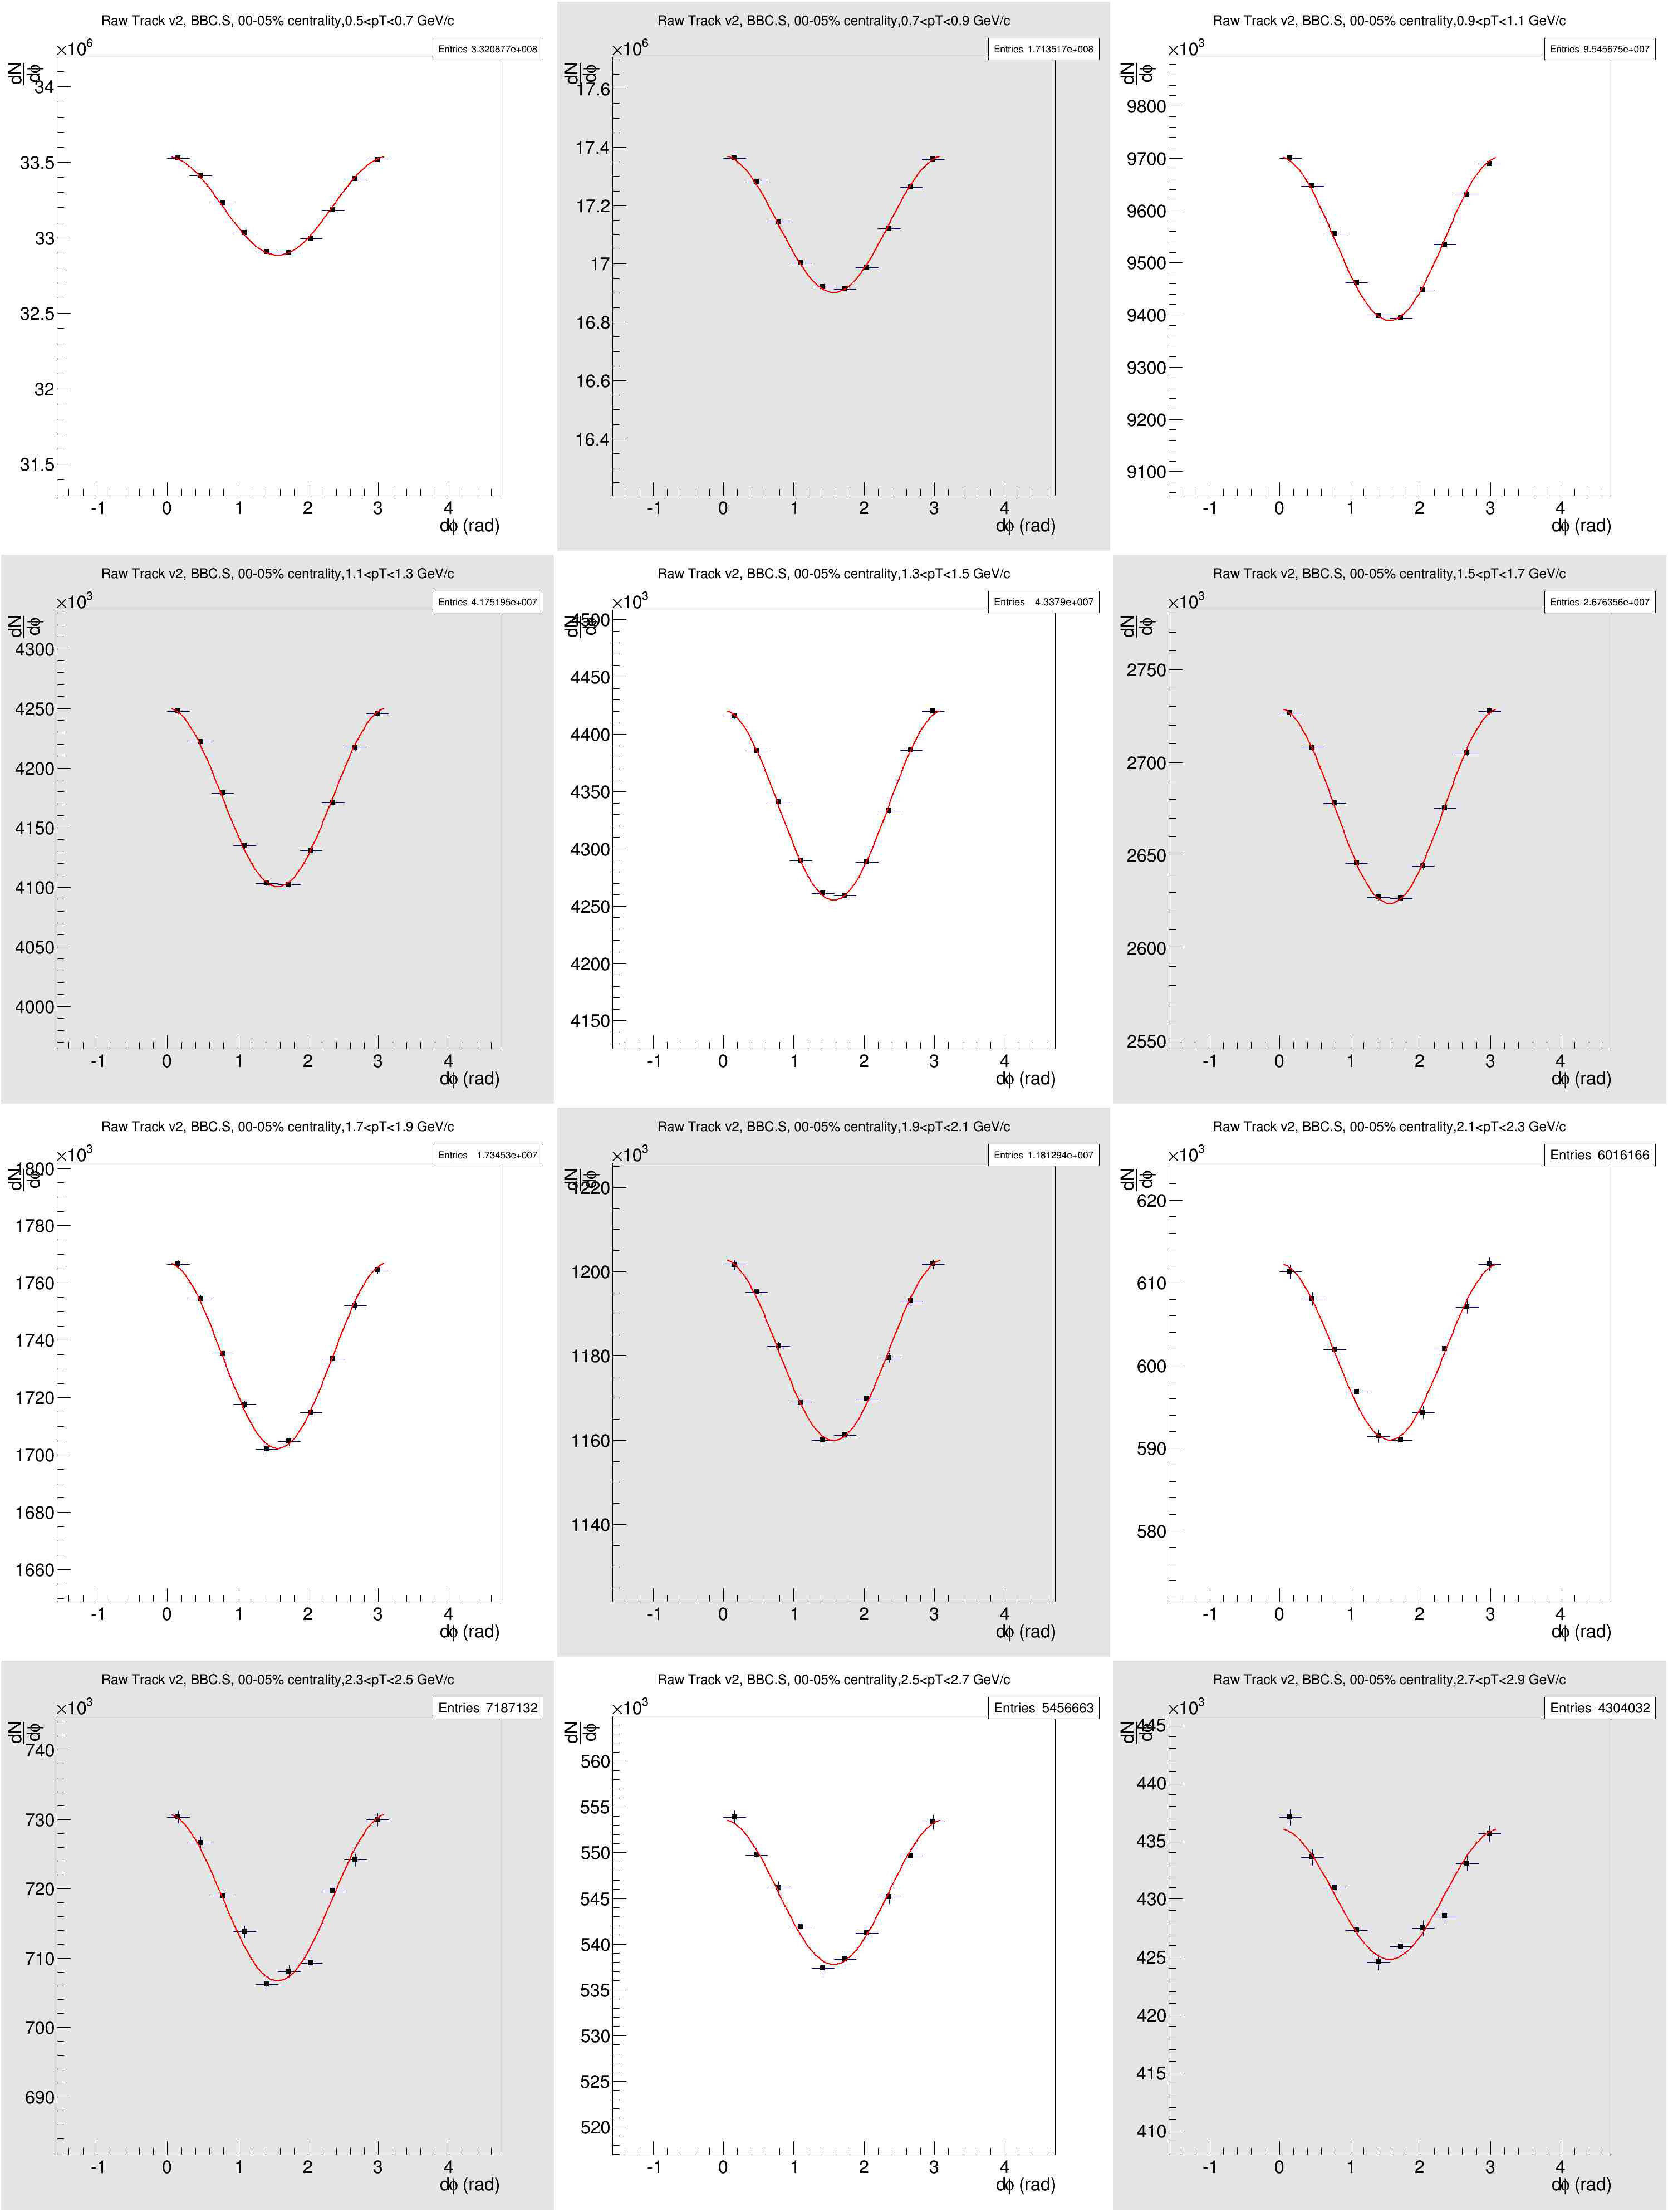
\includegraphics[width=1\textwidth]{chargedtrackv2/htrkdphi2bbcs_0.jpg}
    \rule{35em}{0.5pt}
  \caption[$\frac{dN}{d\phi}$ vs $d\phi$, 0-5\% centrality.]{$\frac{d^N}{d\phi}$ vs $d\phi$, 0-5\% centrality, each plot represents a 0.2 GeV slice in transverse momentum space.}
  \label{fig:Ndphicent0}
\end{figure}

\begin{figure}[htbp!]
  \centering
    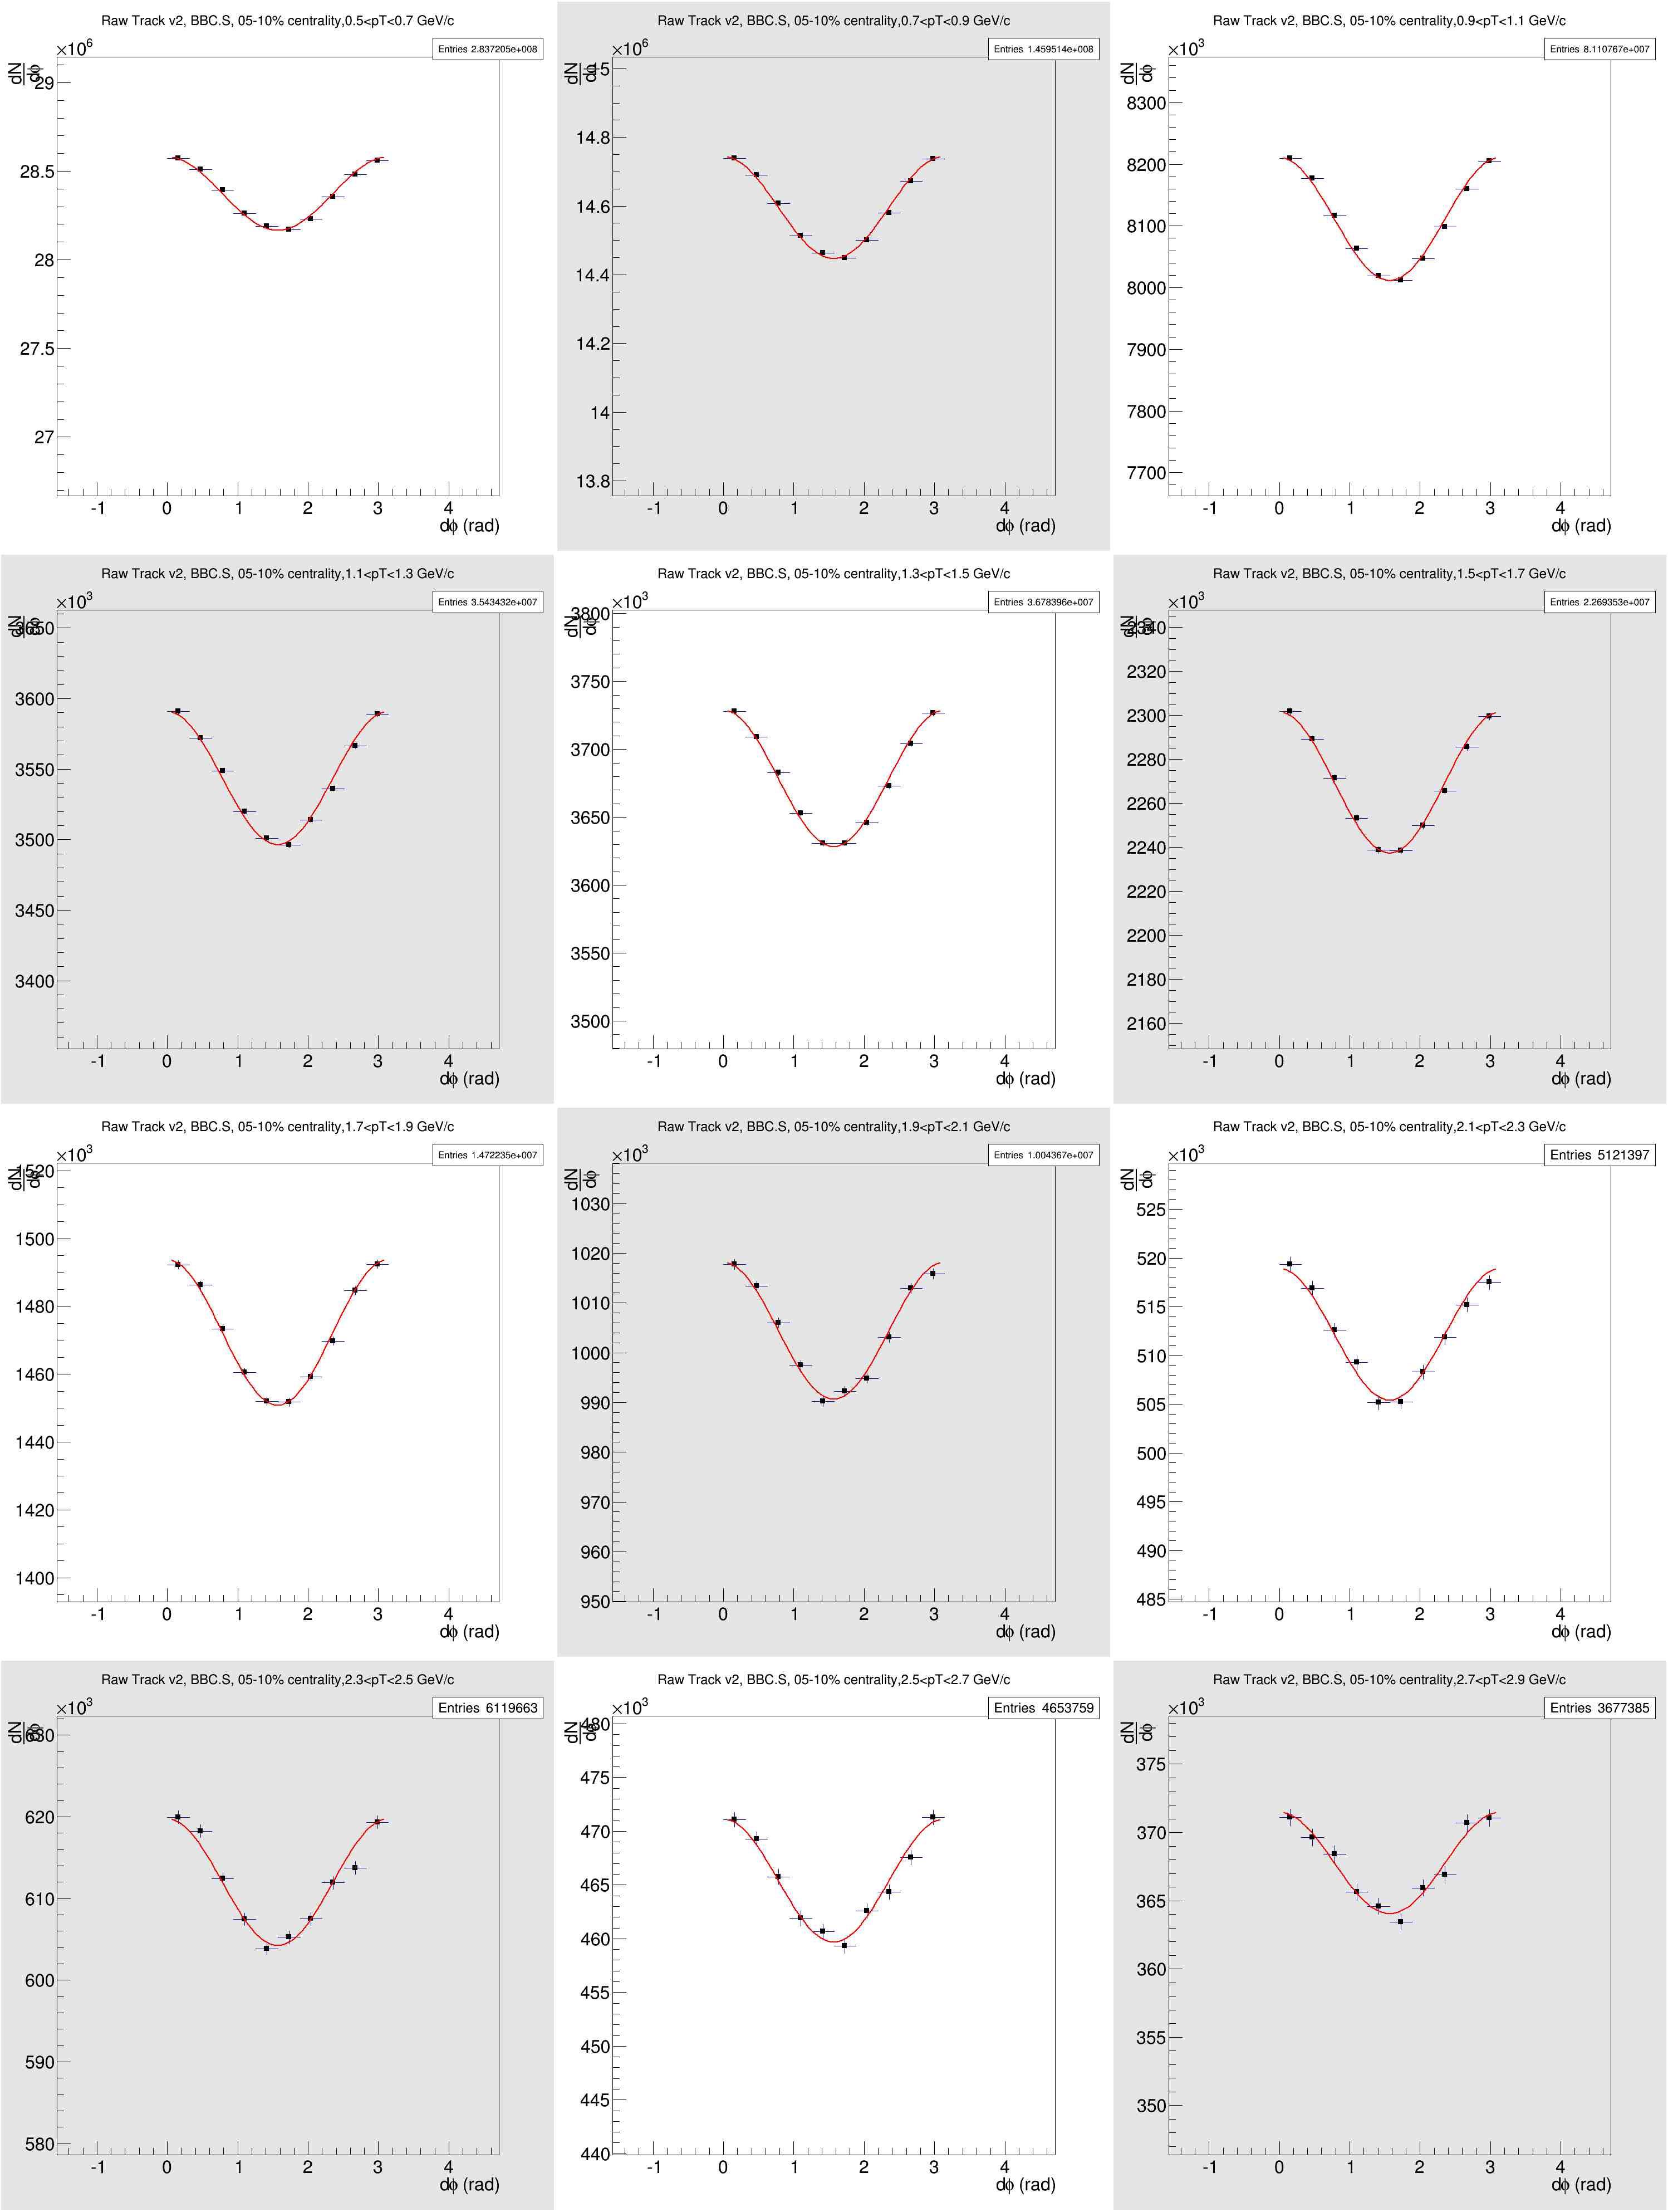
\includegraphics[width=1\textwidth]{chargedtrackv2/htrkdphi2bbcs_1.jpg}
    \rule{35em}{0.5pt}
  \caption[$\frac{dN}{d\phi}$ vs $d\phi$, 5-10\% centrality.]{$\frac{d^N}{d\phi}$ vs $d\phi$, 5-10\% centrality, each plot represents a 0.2 GeV slice in transverse momentum space.}
  \label{fig:Ndphicent1}
\end{figure}
\begin{figure}[htbp!]
  \centering
    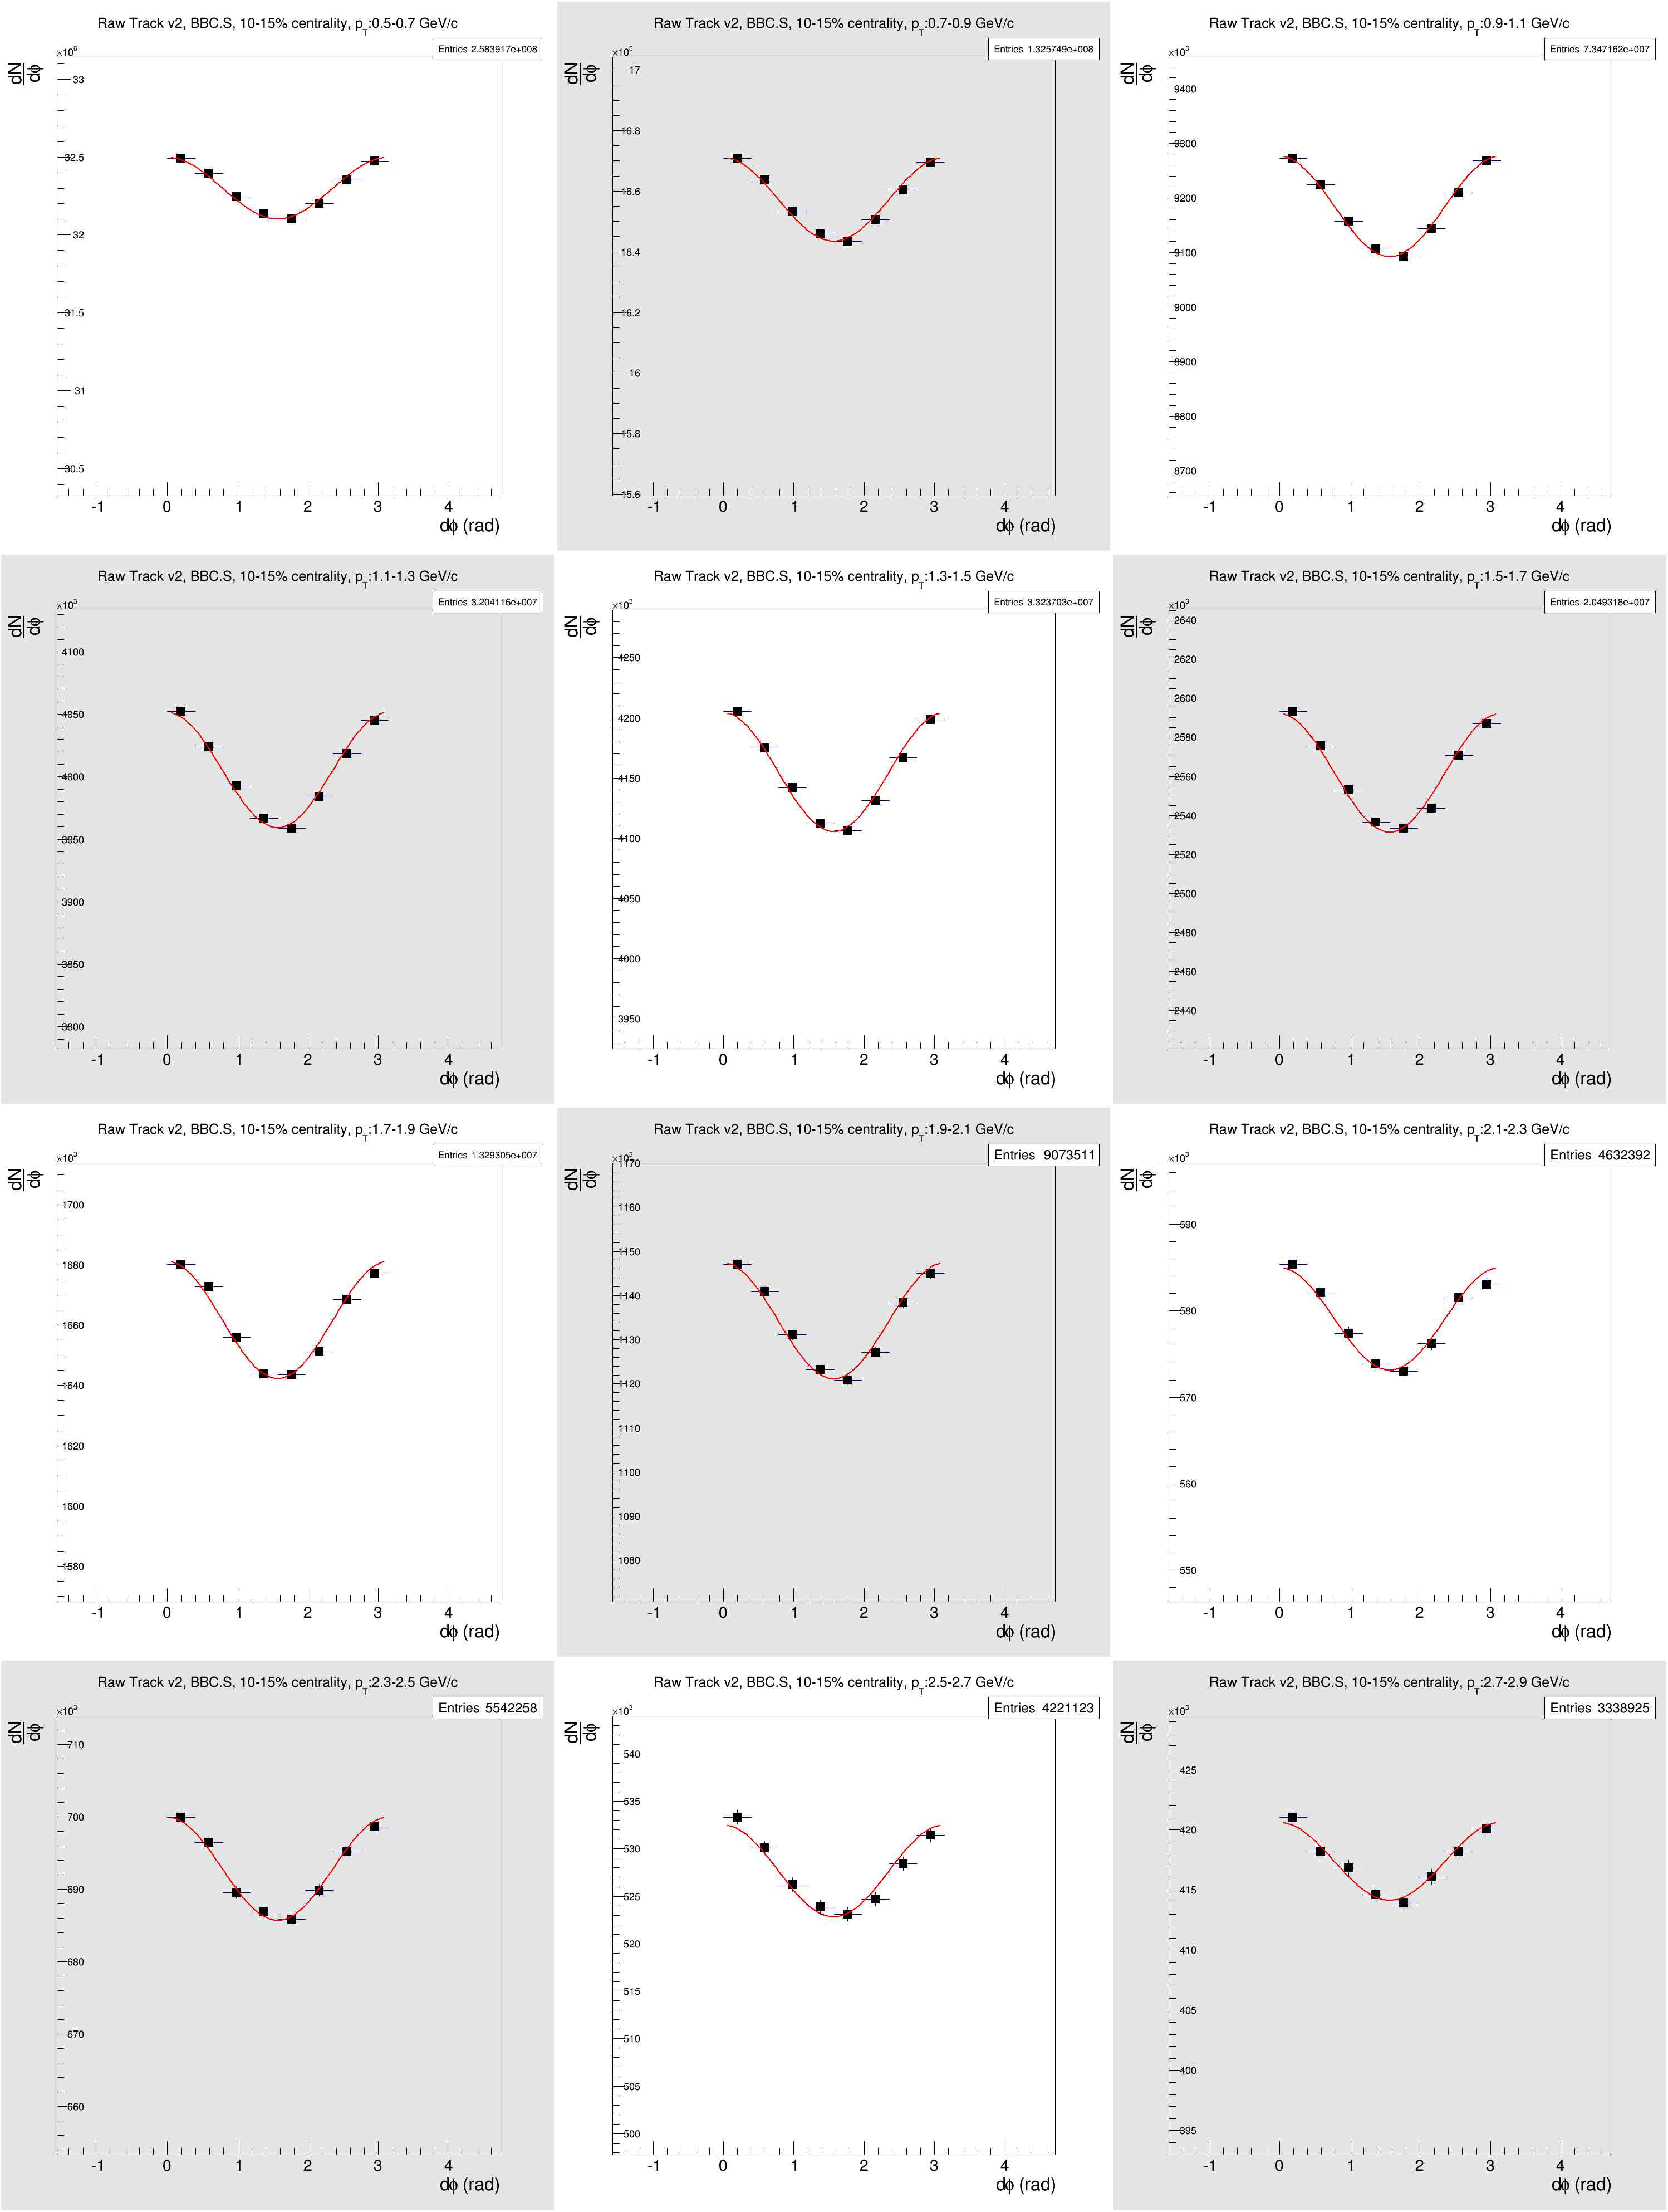
\includegraphics[width=1\textwidth]{chargedtrackv2/htrkdphi2bbcs_2.jpg}
    \rule{35em}{0.5pt}
  \caption[$\frac{dN}{d\phi}$ vs $d\phi$, 10-15\% centrality.]{$\frac{d^N}{d\phi}$ vs $d\phi$, 10-15\% centrality, each plot represents a 0.2 GeV slice in transverse momentum space.}
  \label{fig:Ndphicent2}
\end{figure}
\begin{figure}[htbp!]
  \centering
    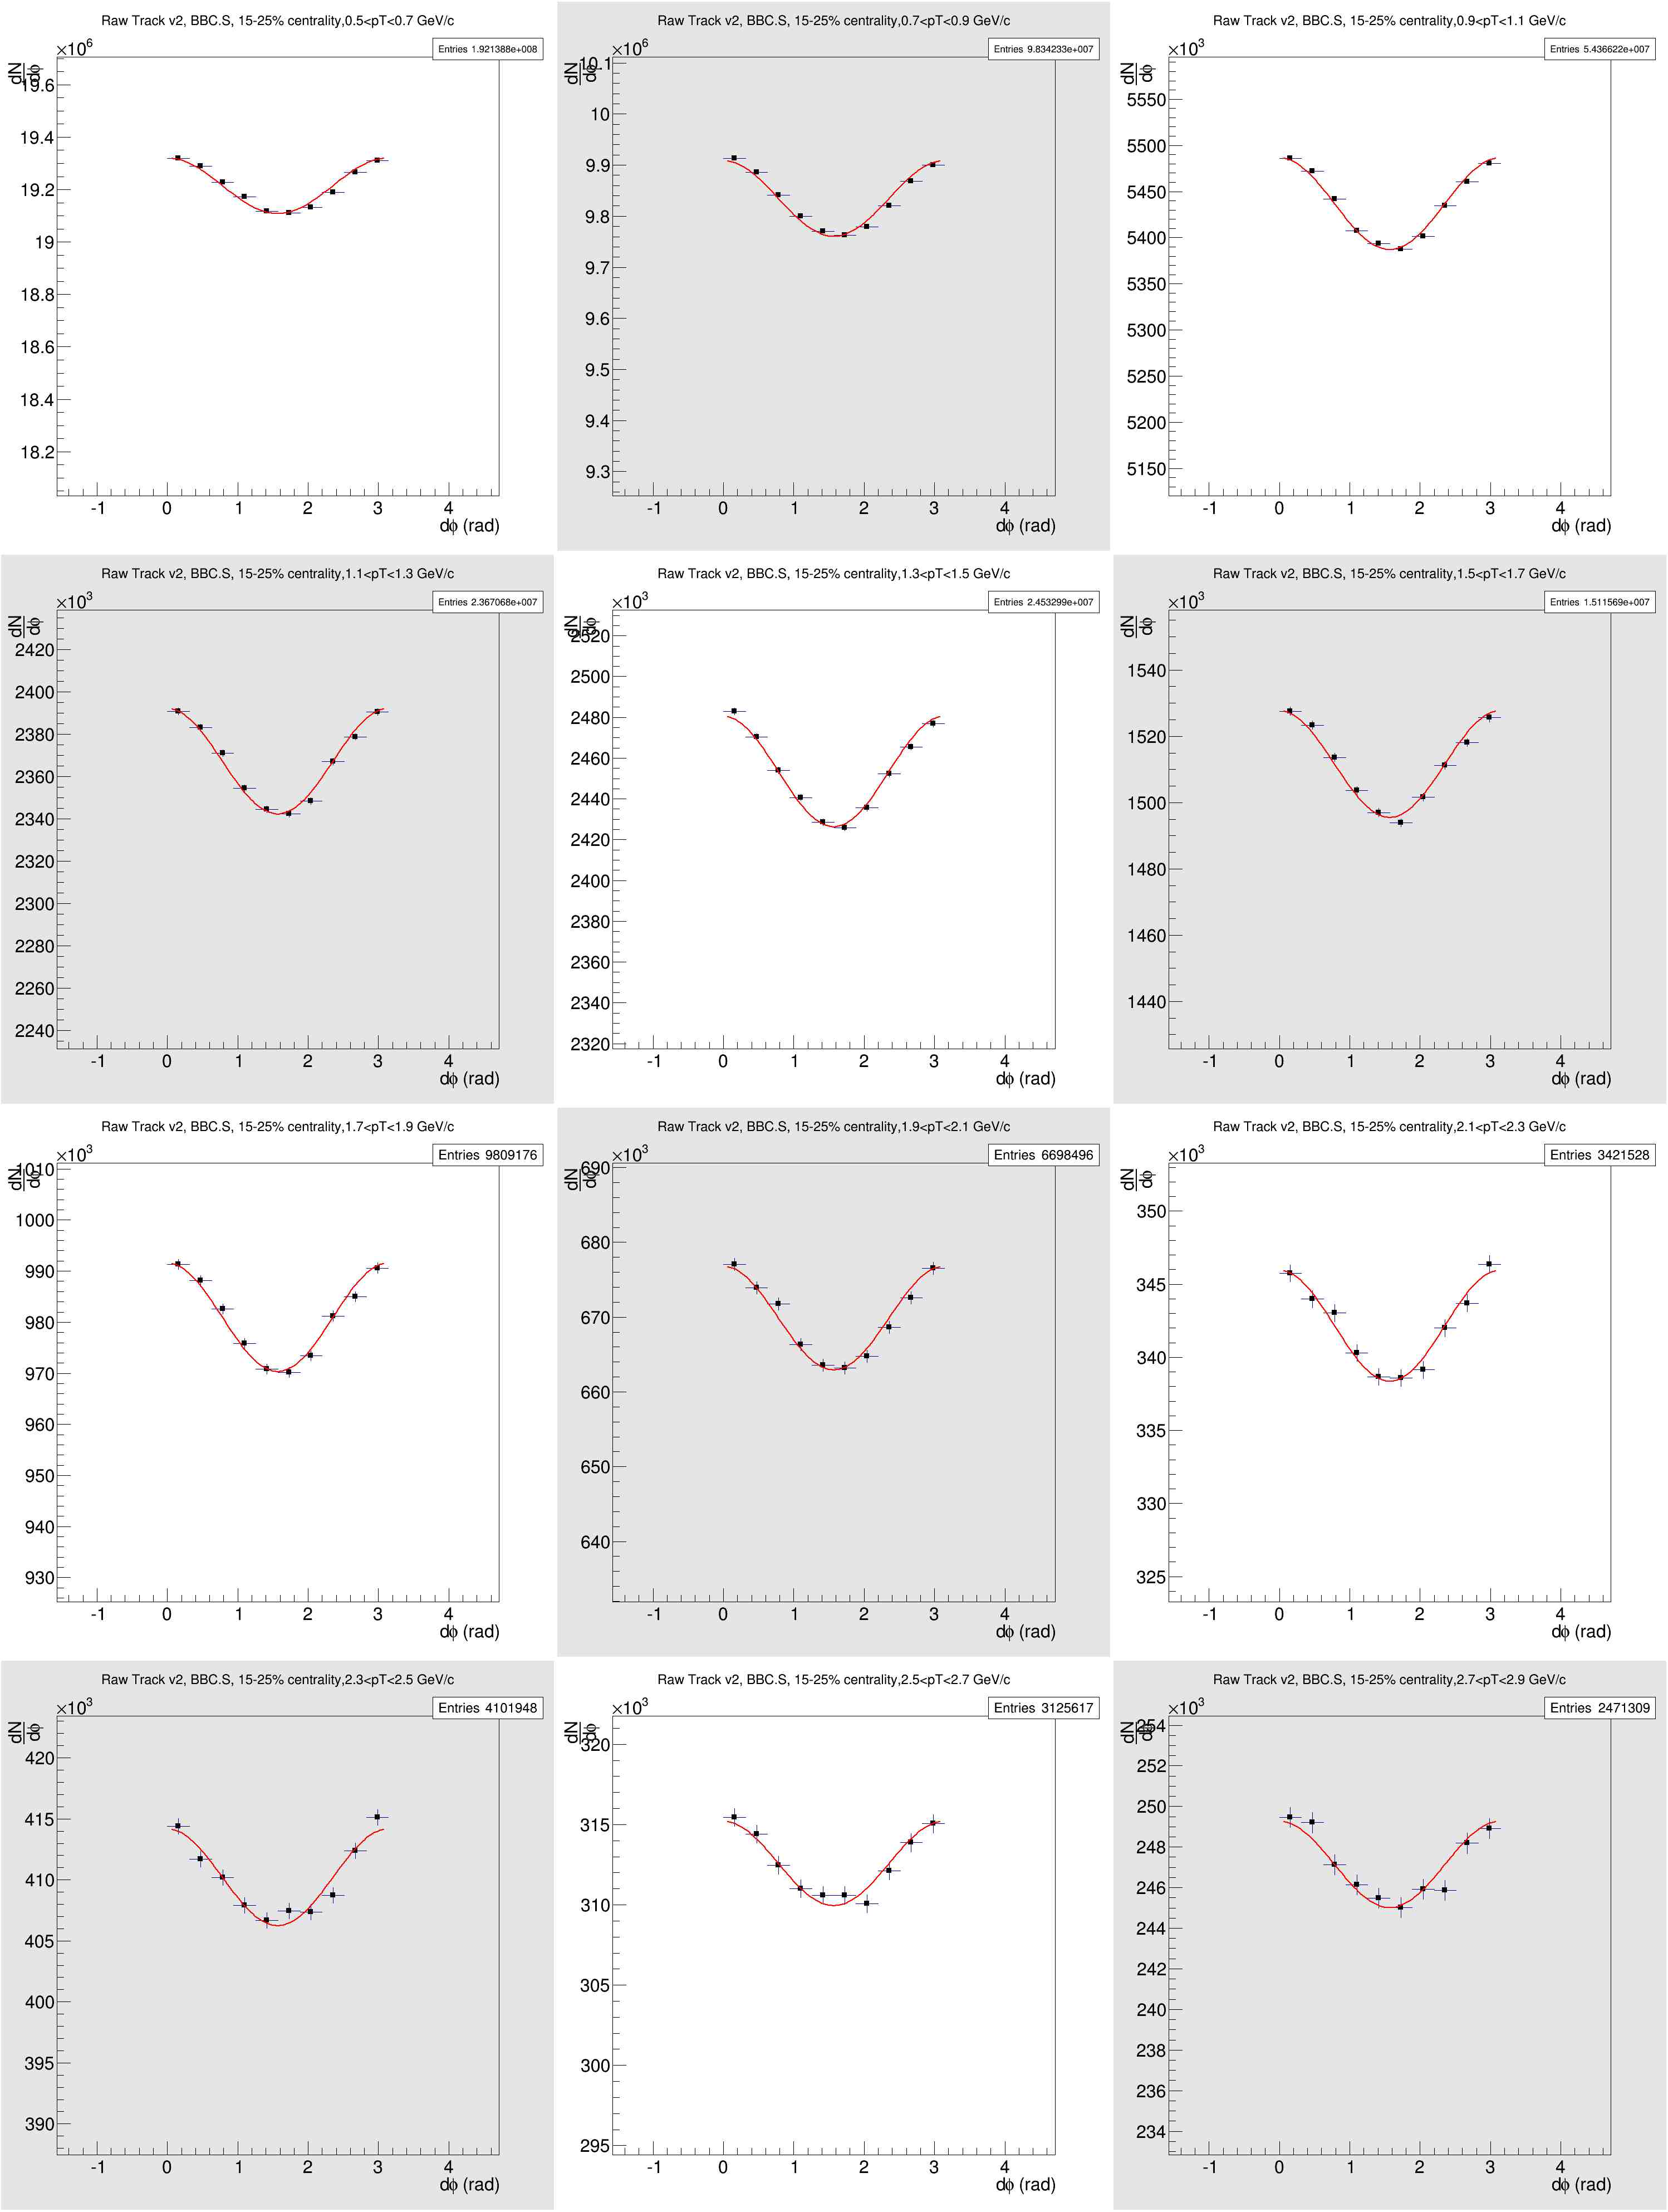
\includegraphics[width=1\textwidth]{chargedtrackv2/htrkdphi2bbcs_3.jpg}
    \rule{35em}{0.5pt}
  \caption[$\frac{dN}{d\phi}$ vs $d\phi$, 15-25\% centrality.]{$\frac{d^N}{d\phi}$ vs $d\phi$, 15-25\% centrality, each plot represents a 0.2 GeV slice in transverse momentum space.}
  \label{fig:Ndphicent3}
\end{figure}

\section{Particle Identification: TOFW}

\subsection{Single Gaussian fits, $p_T$=0.5-1.3 GeV/c, TOF.W, negative charged tracks}
\label{app:singlegauss}
\begin{figure}[H]
  \centering
    \begin{subfigure}{1\textwidth}
    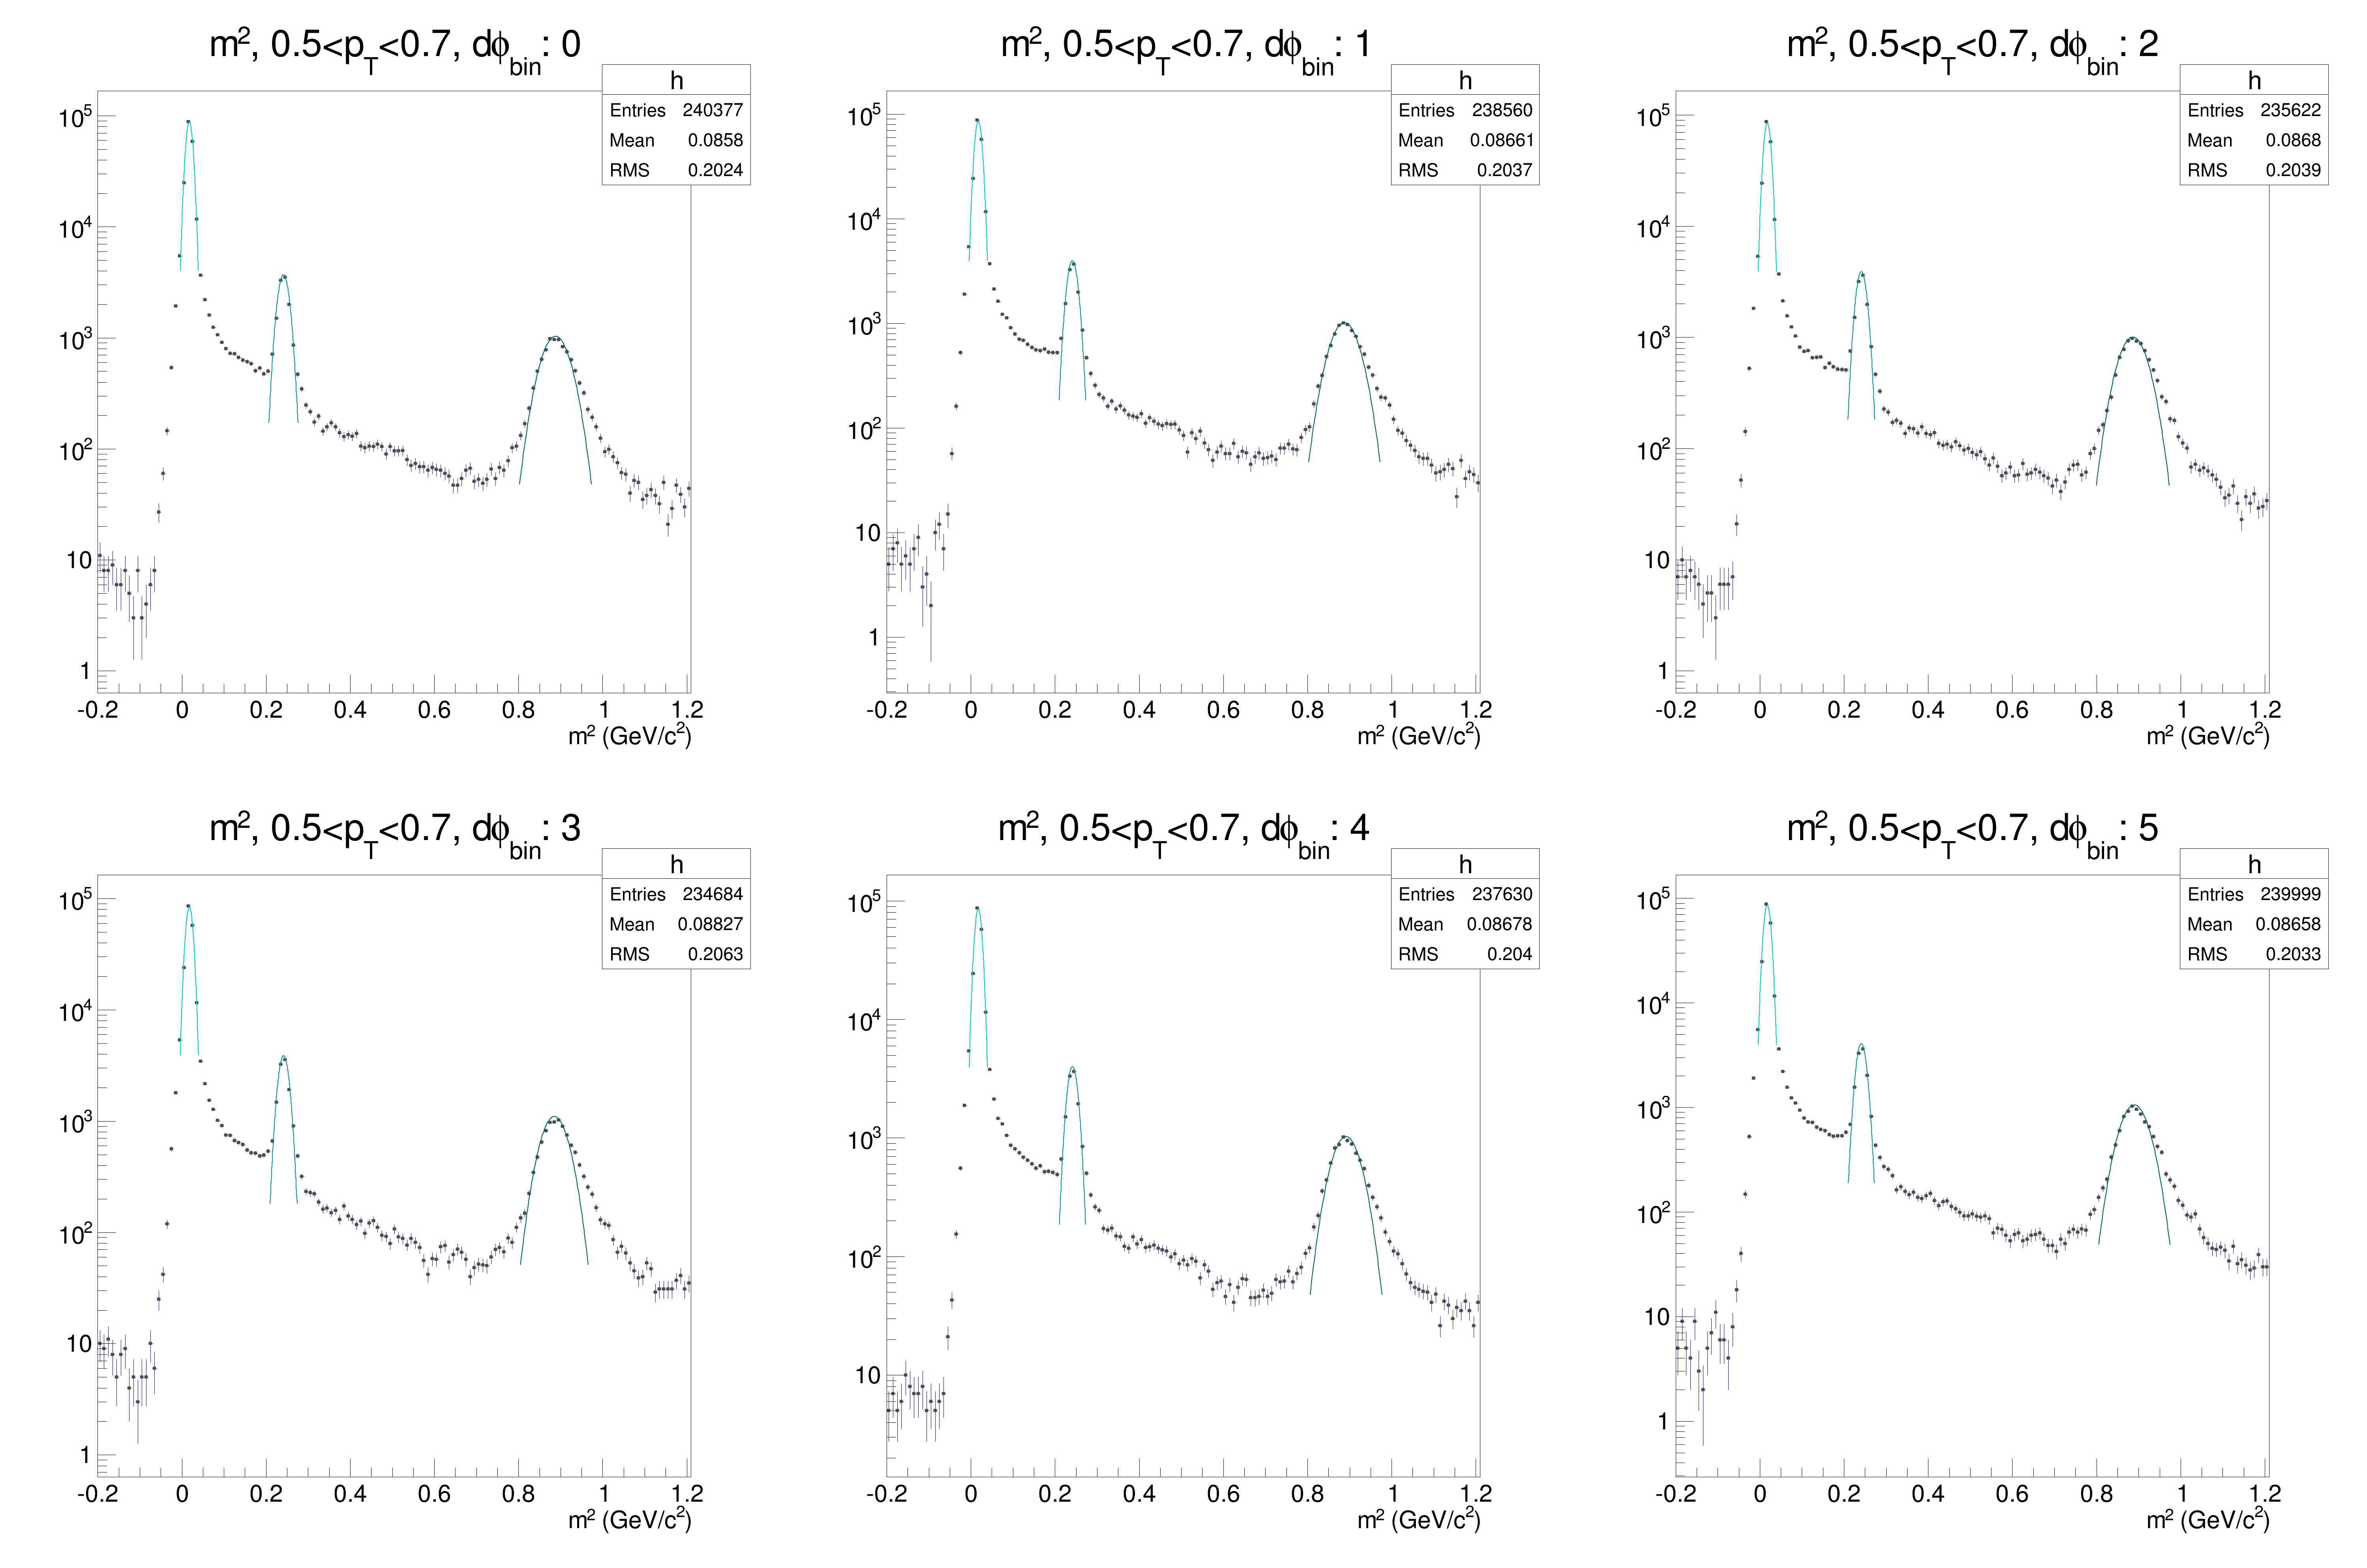
\includegraphics[width=1\textwidth]{lowptfits/yieldvsdphi_tof1_cent0_ch0_pT-5-7.jpg}
    \end{subfigure}
    \begin{subfigure}{1\textwidth}
    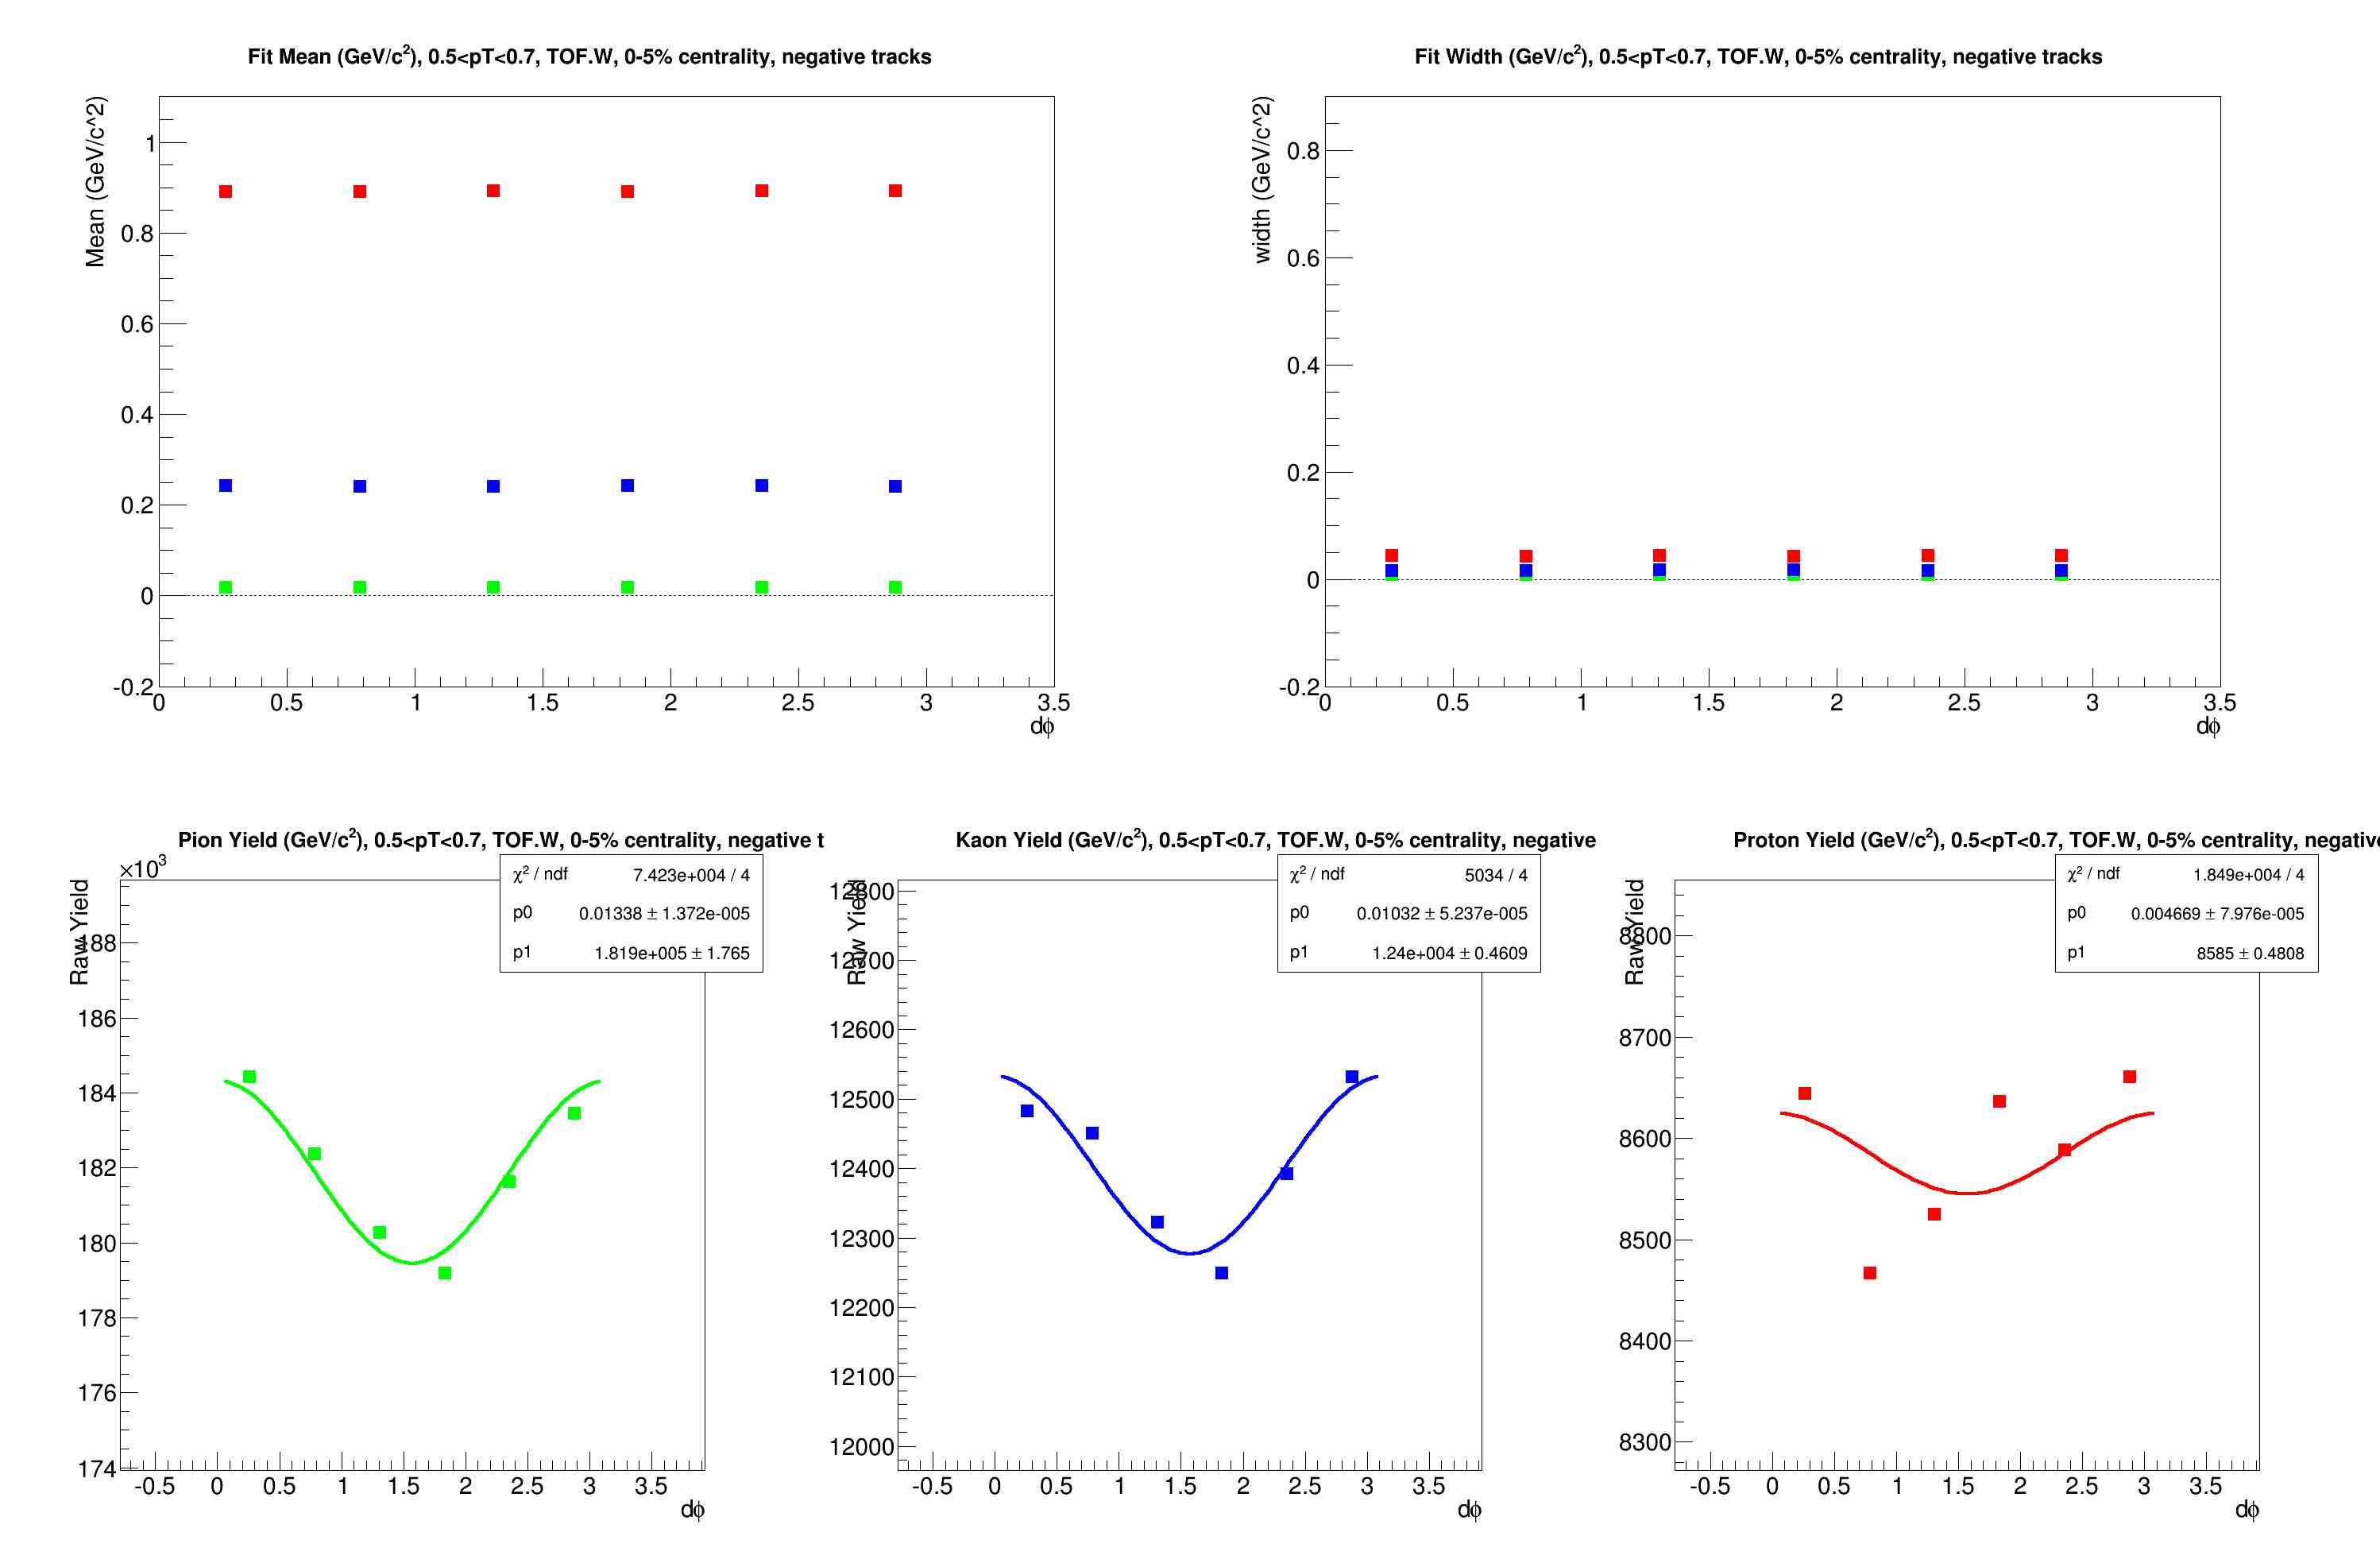
\includegraphics[width=1\textwidth]{lowptfits/fitParams_tof1_cent0_ch0_pT-5-7.jpg}
    \end{subfigure}
    \rule{35em}{0.5pt}
  \caption[PID fits and Yield vs $d\phi$ for $p_T$=0.5-0.7 GeV/c, TOF.W, negative particles ]{$m^2$ Gaussian fits for PID and resulting Yield vs $d\phi$ for $p_T$=0.5-0.7 GeV/c, TOF.W, negative particles}
  \label{fig:fits5-7neg}
\end{figure}

\begin{figure}[H]
  \centering
    \begin{subfigure}{1\textwidth}
    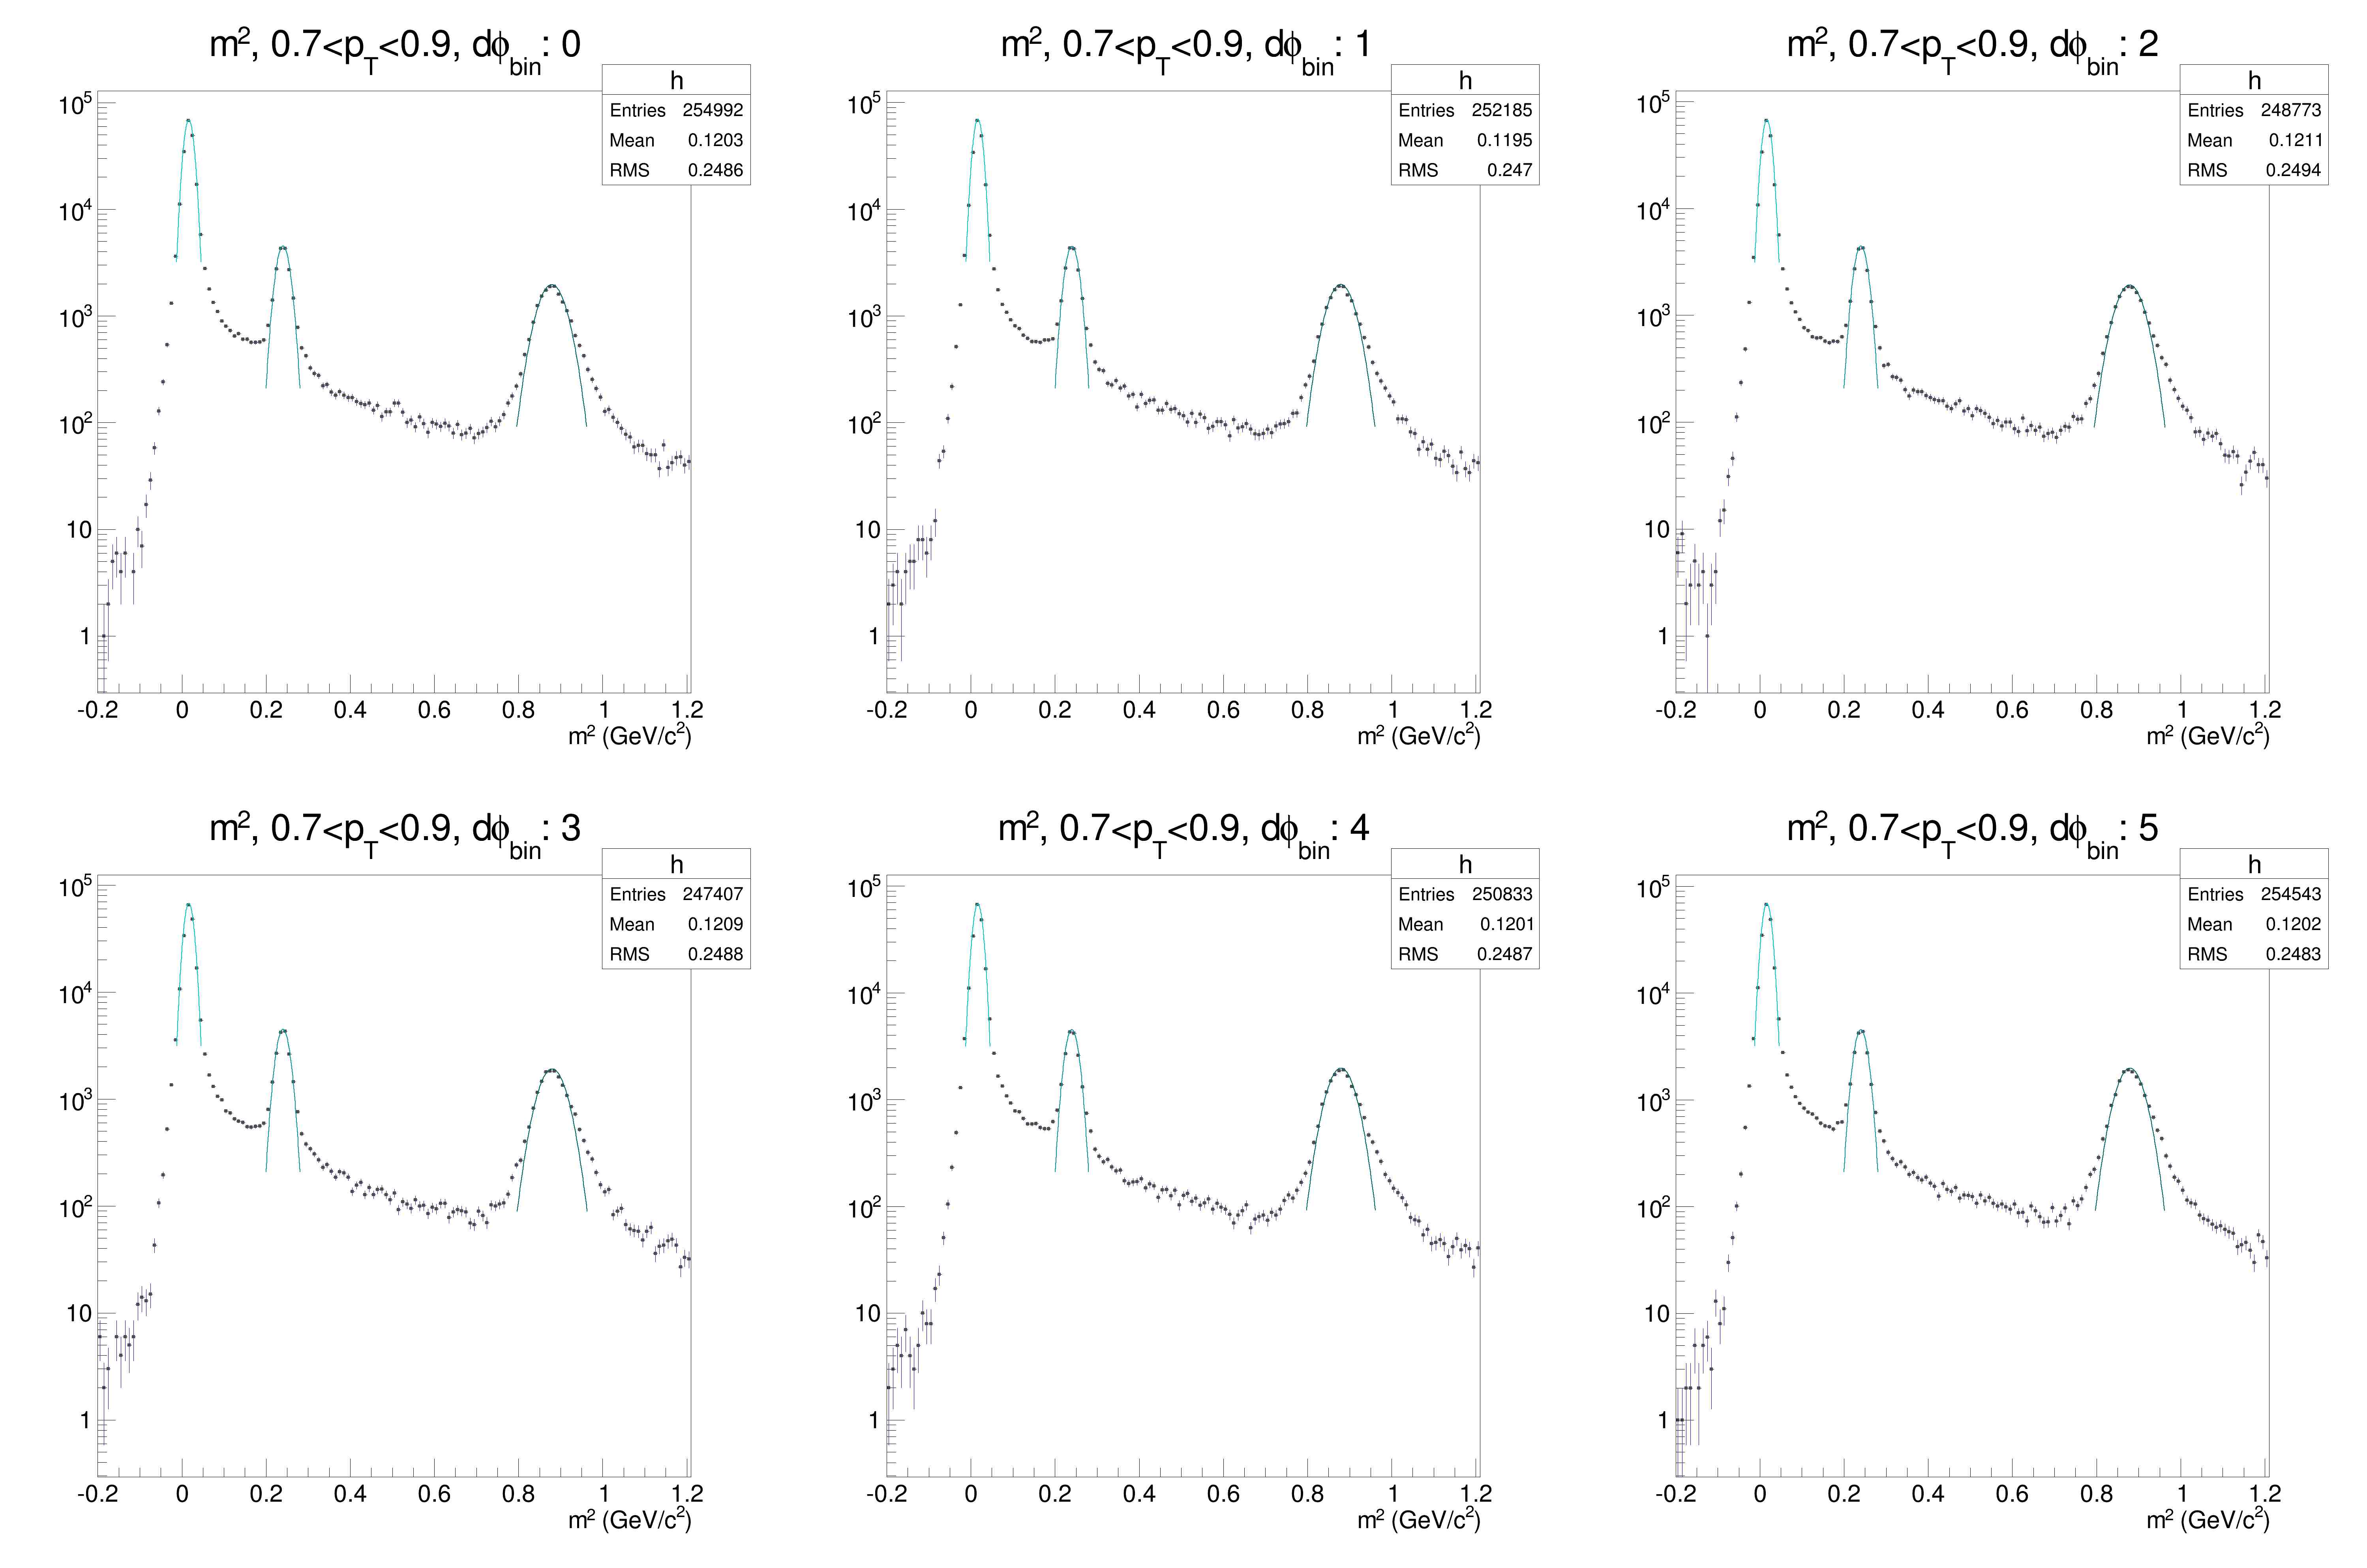
\includegraphics[width=1\textwidth]{lowptfits/yieldvsdphi_tof1_cent0_ch0_pT-7-9.jpg}
    \end{subfigure}
    \begin{subfigure}{1\textwidth}
    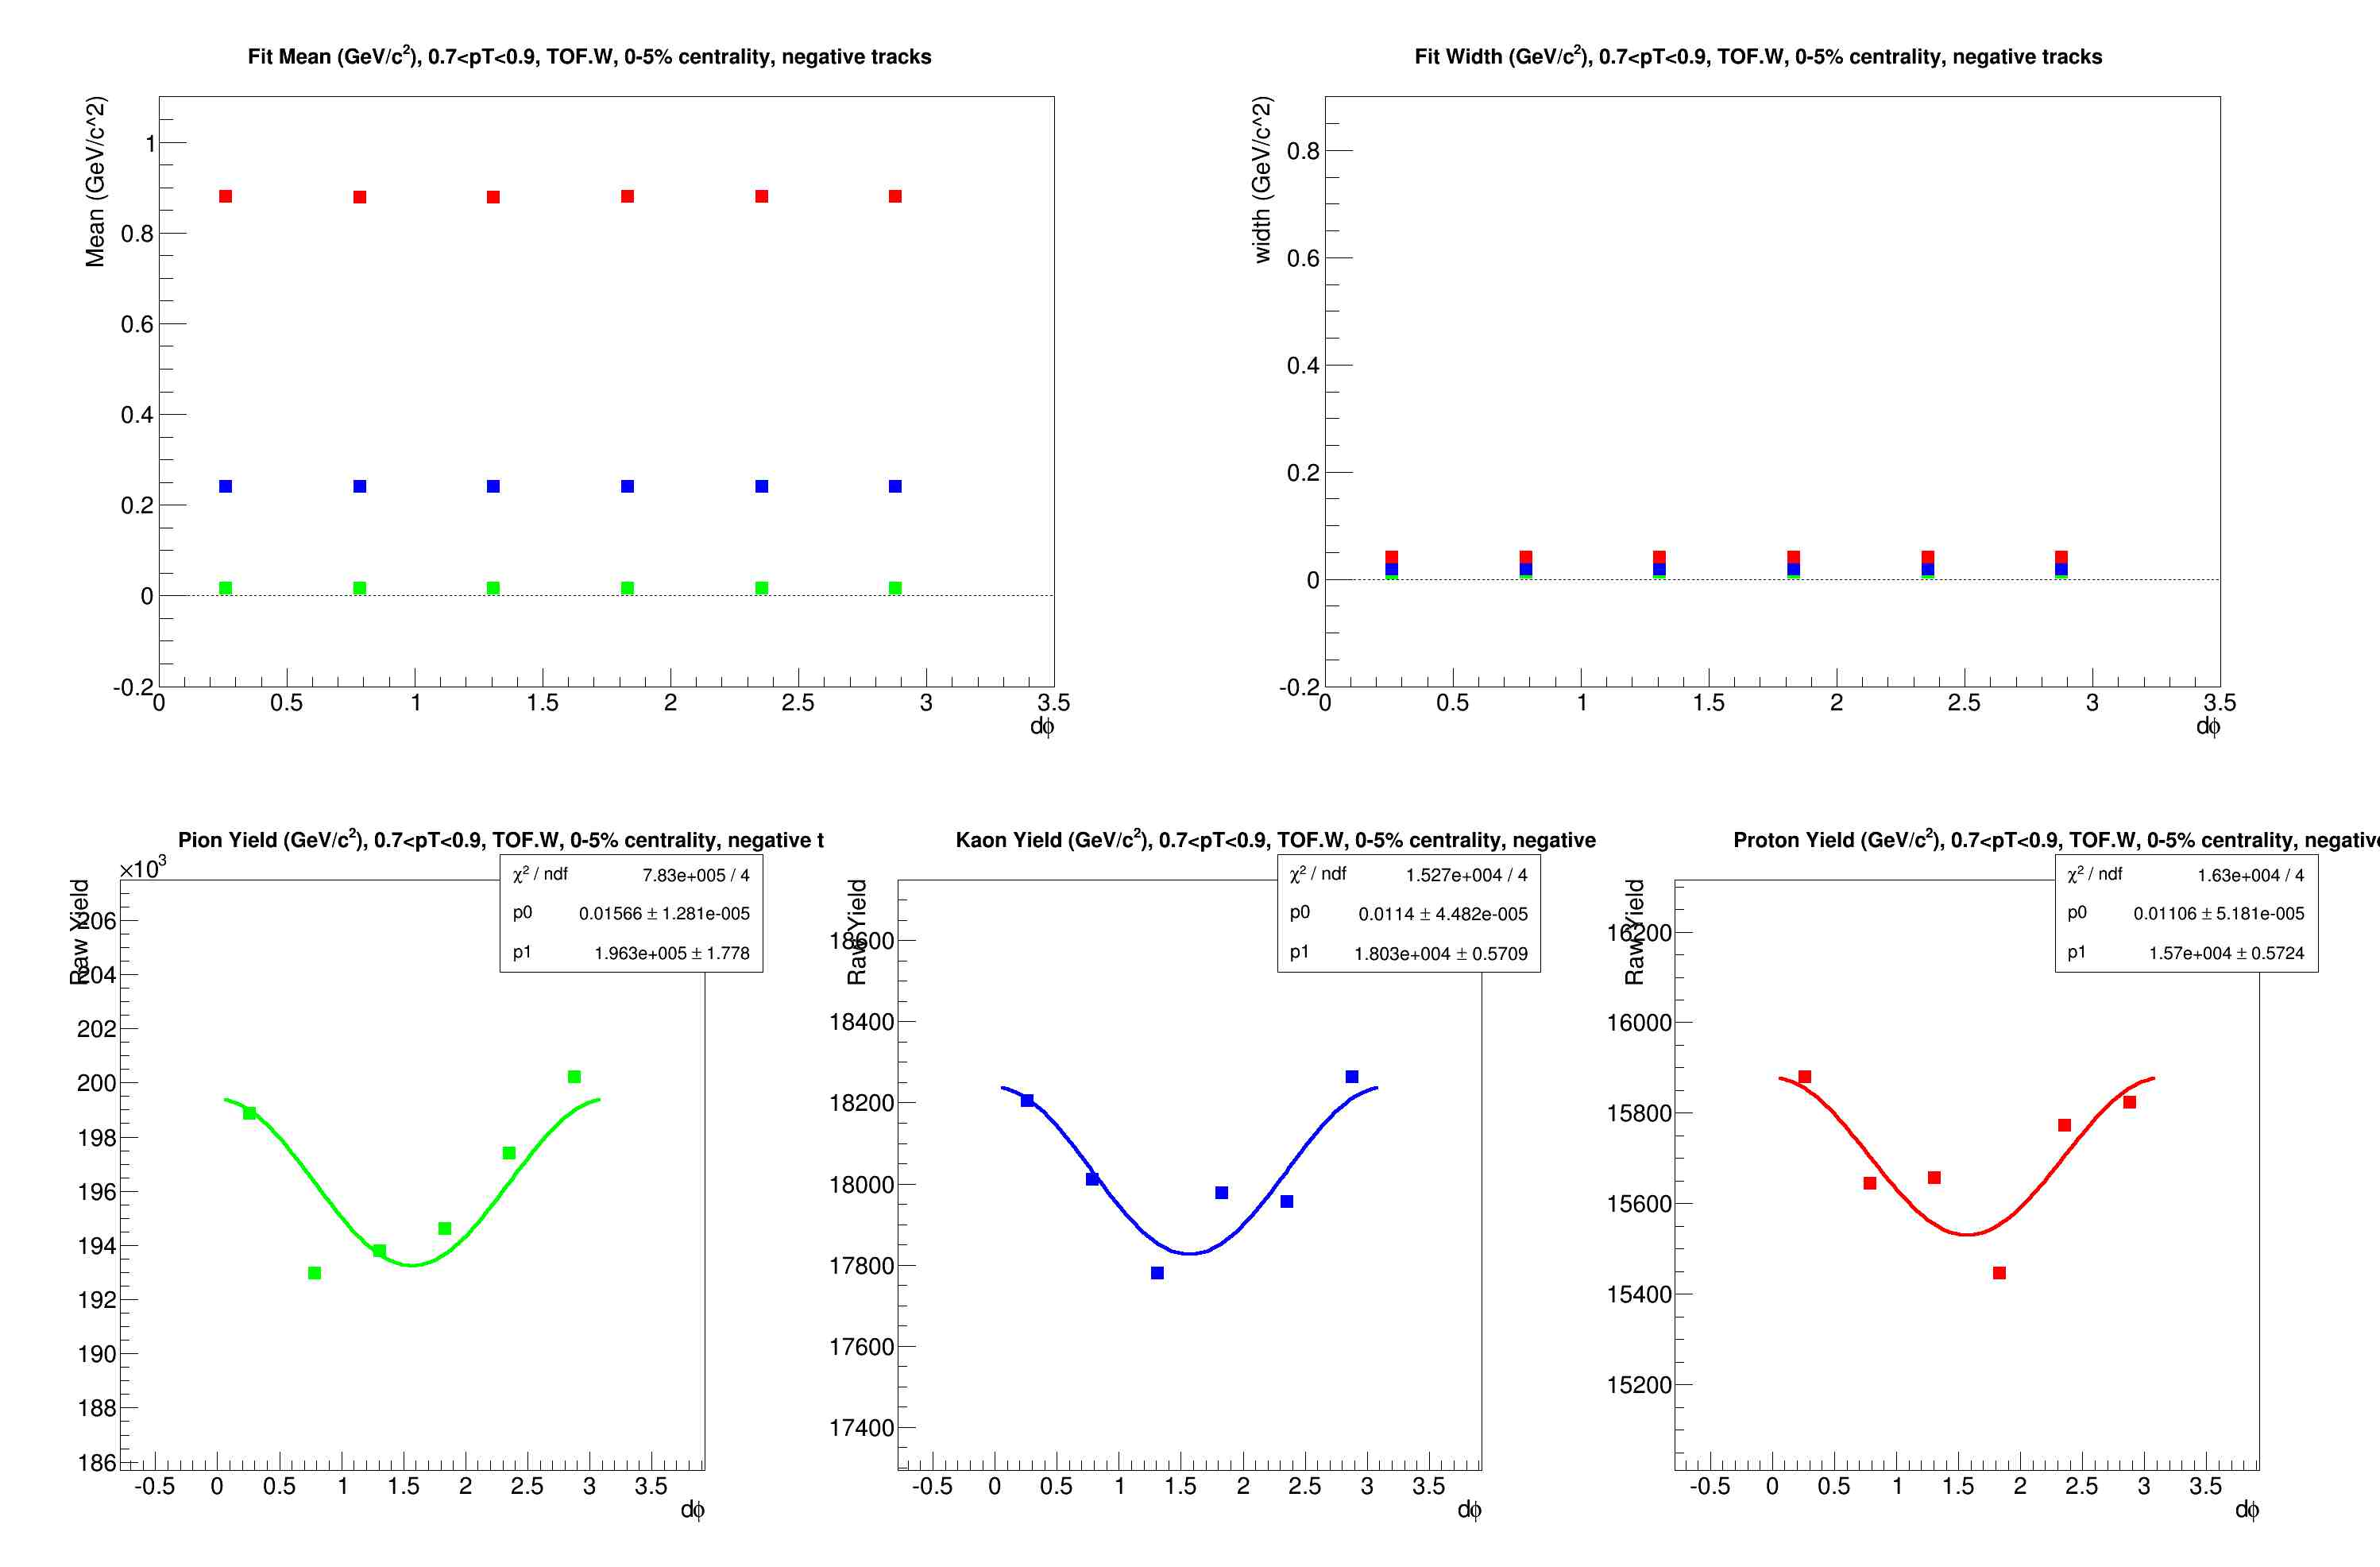
\includegraphics[width=1\textwidth]{lowptfits/fitParams_tof1_cent0_ch0_pT-7-9.jpg}
    \end{subfigure}
    \rule{35em}{0.5pt}
  \caption[PID fits and Yield vs $d\phi$ for $p_T$=0.7-0.9 GeV/c, TOF.W, negative particles ]{$m^2$ Gaussian fits for PID and resulting Yield vs $d\phi$ for $p_T$=0.7-0.9 GeV/c, TOF.W, negative particles}
  \label{fig:fits7-9neg}
\end{figure}

\begin{figure}[H]
  \centering
    \begin{subfigure}[p]{1\textwidth}
    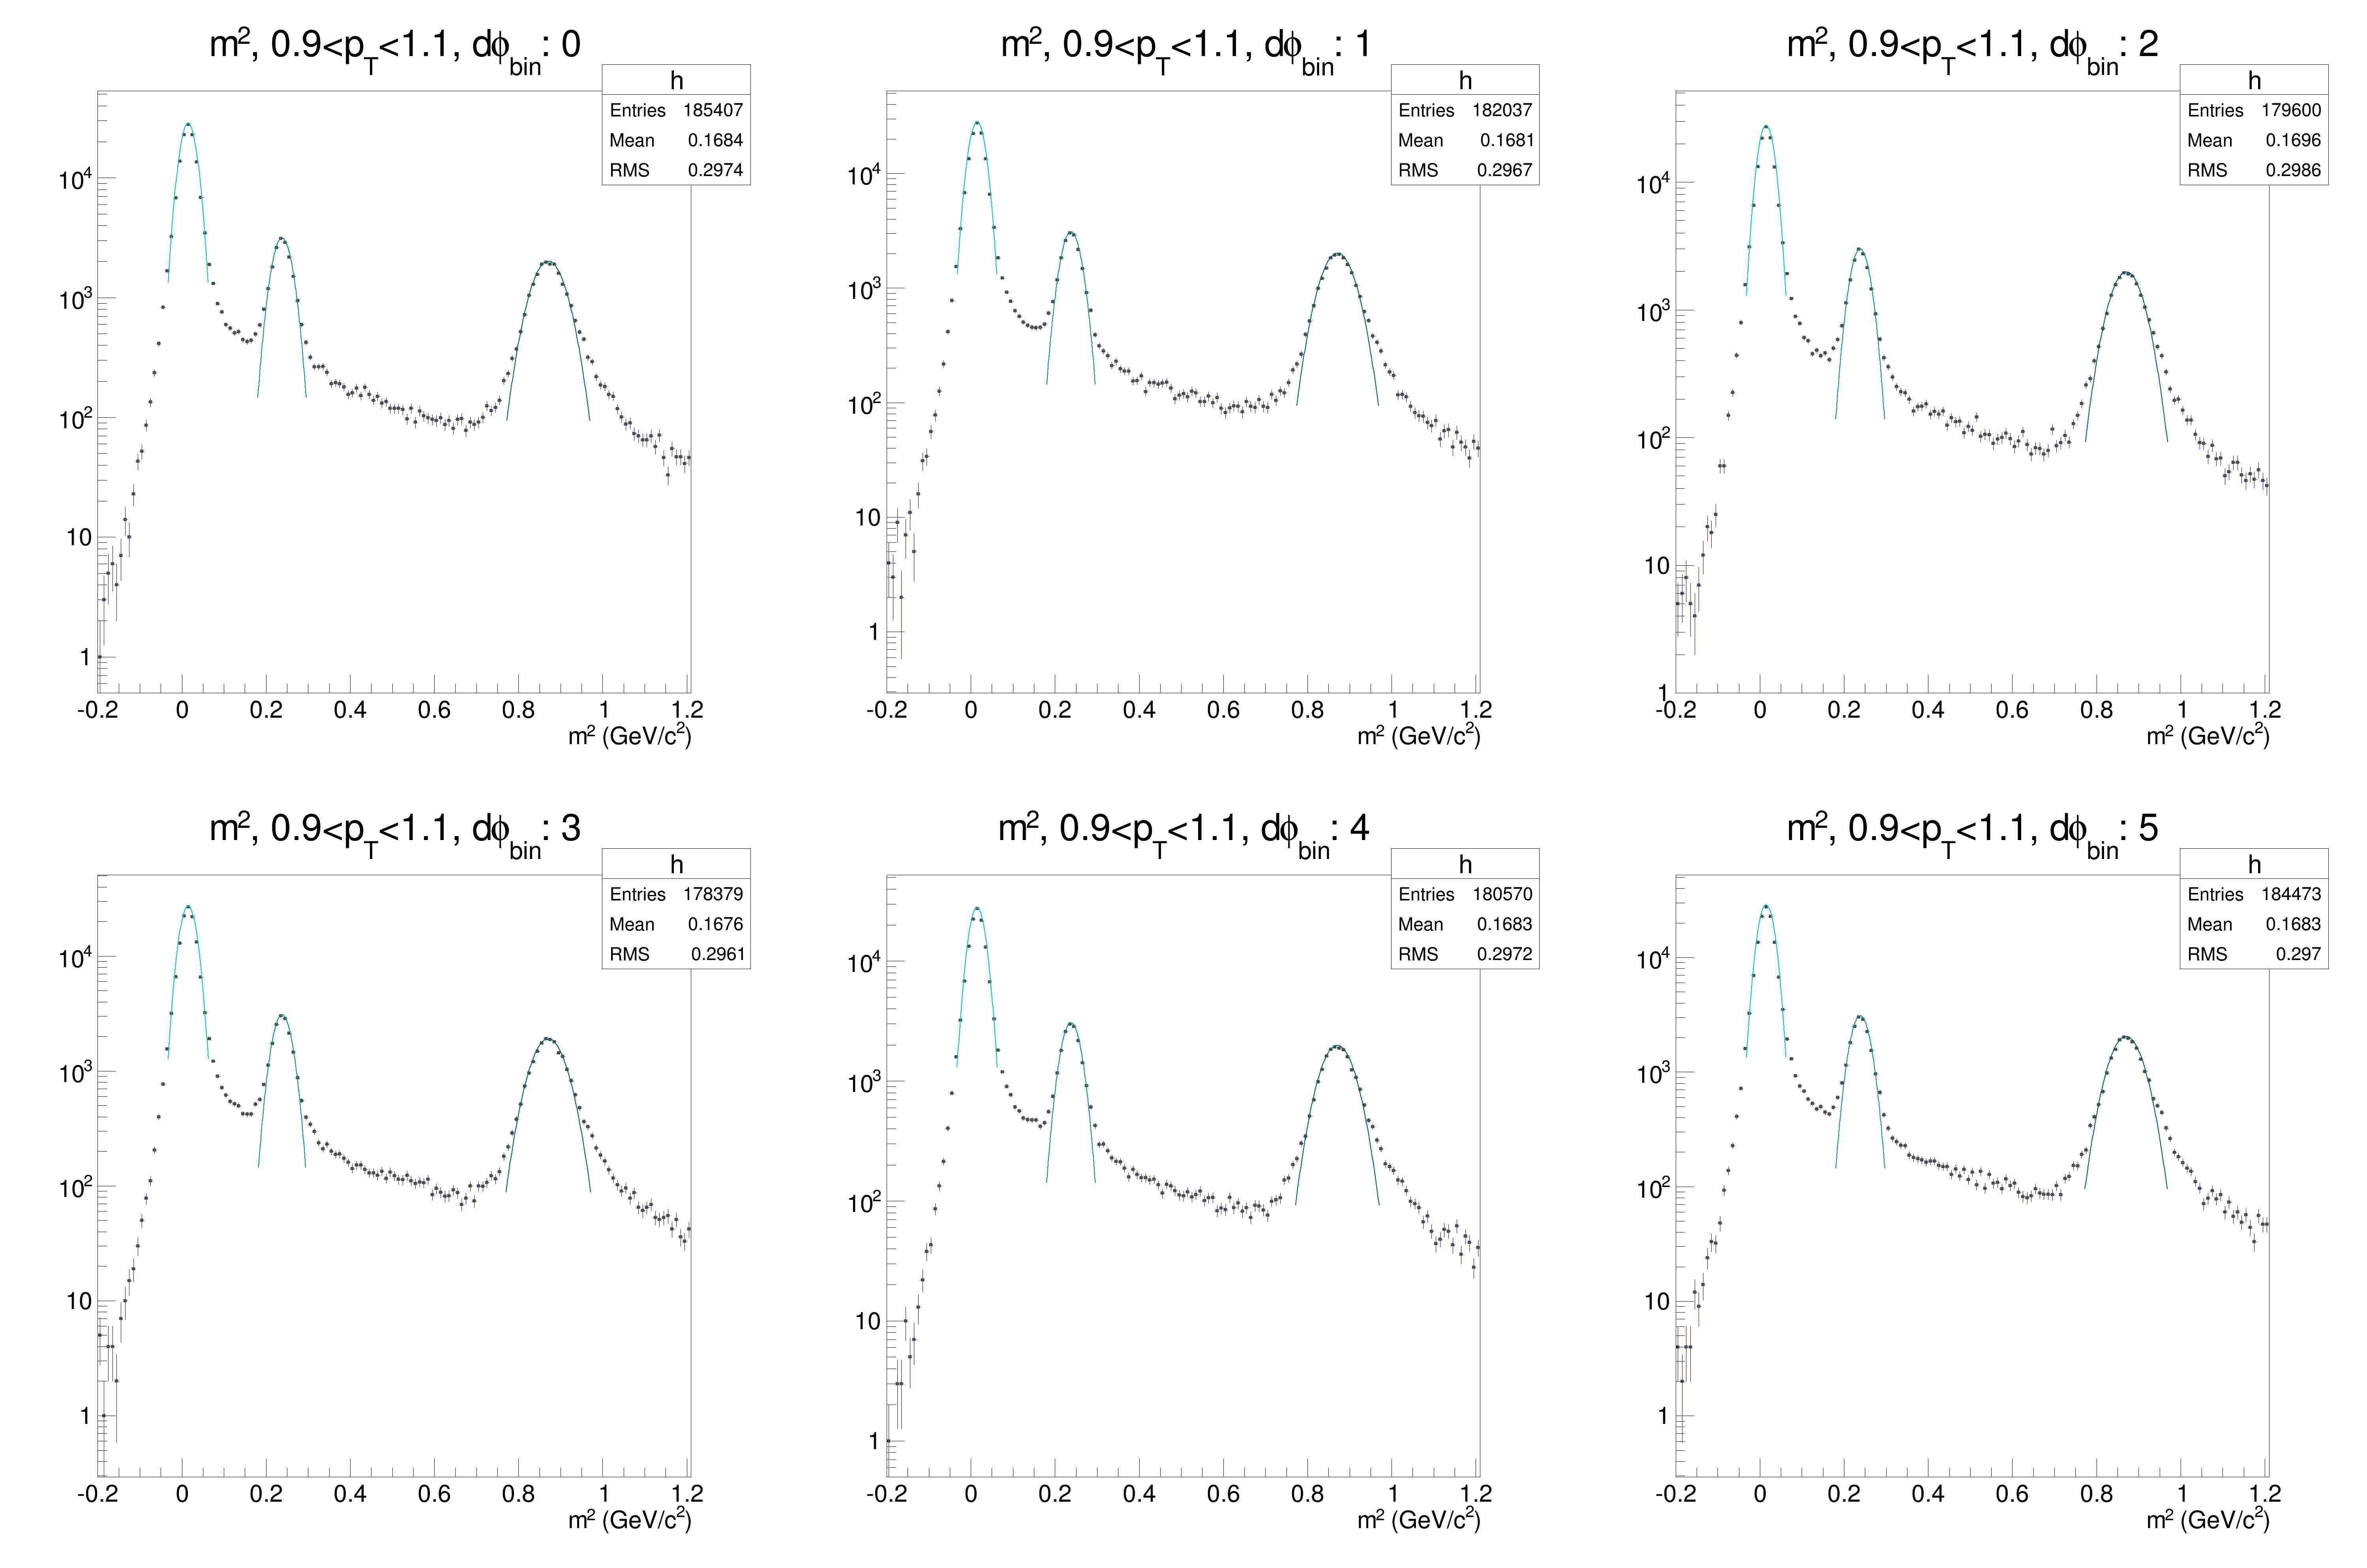
\includegraphics[width=1\textwidth]{lowptfits/yieldvsdphi_tof1_cent0_ch0_pT-9-11.jpg}
    \end{subfigure}
    \begin{subfigure}[p]{1\textwidth}
    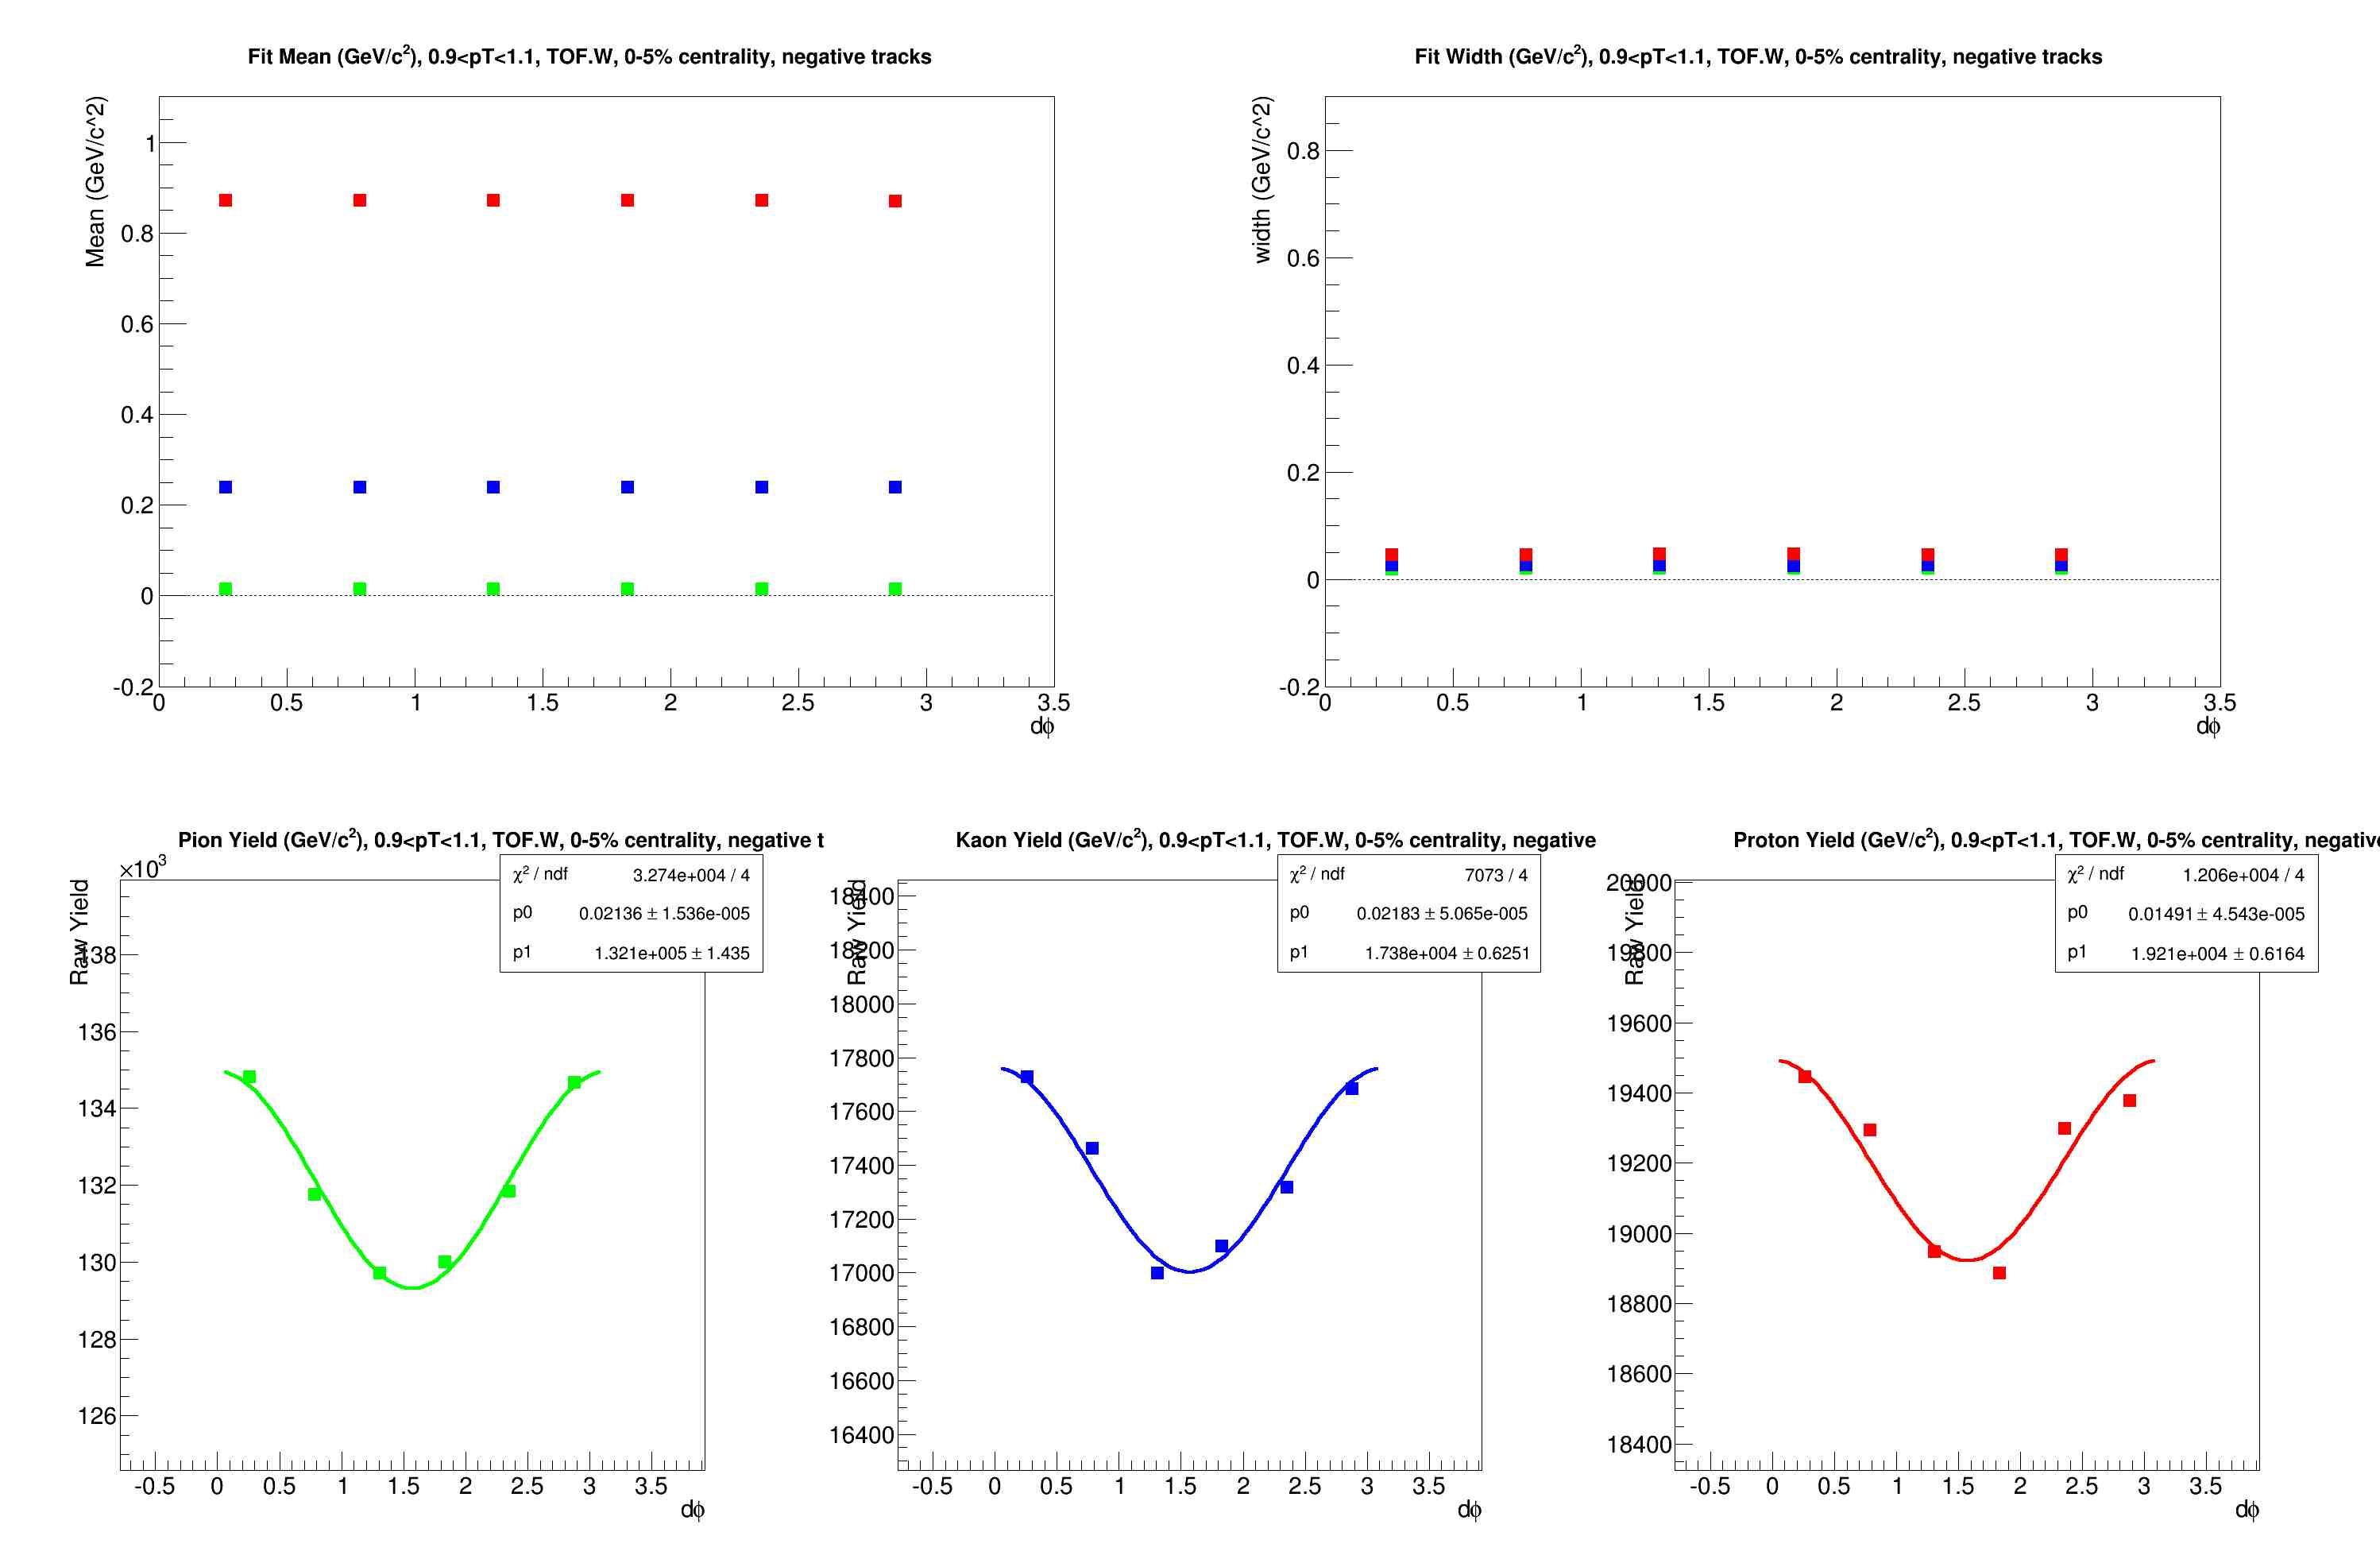
\includegraphics[width=1\textwidth]{lowptfits/fitParams_tof1_cent0_ch0_pT-9-11.jpg}
    \end{subfigure}
    \rule{35em}{0.5pt}
  \caption[PID fits and Yield vs $d\phi$ for $p_T$=0.9-1.1 GeV/c, TOF.W, negative particles ]{$m^2$ Gaussian fits for PID and resulting Yield vs $d\phi$ for $p_T$=0.9-1.1 GeV/c, TOF.W, negative particles}
  \label{fig:fits9-11neg}
\end{figure}

\begin{figure}[H]
  \centering
    \begin{subfigure}[p]{1\textwidth}
    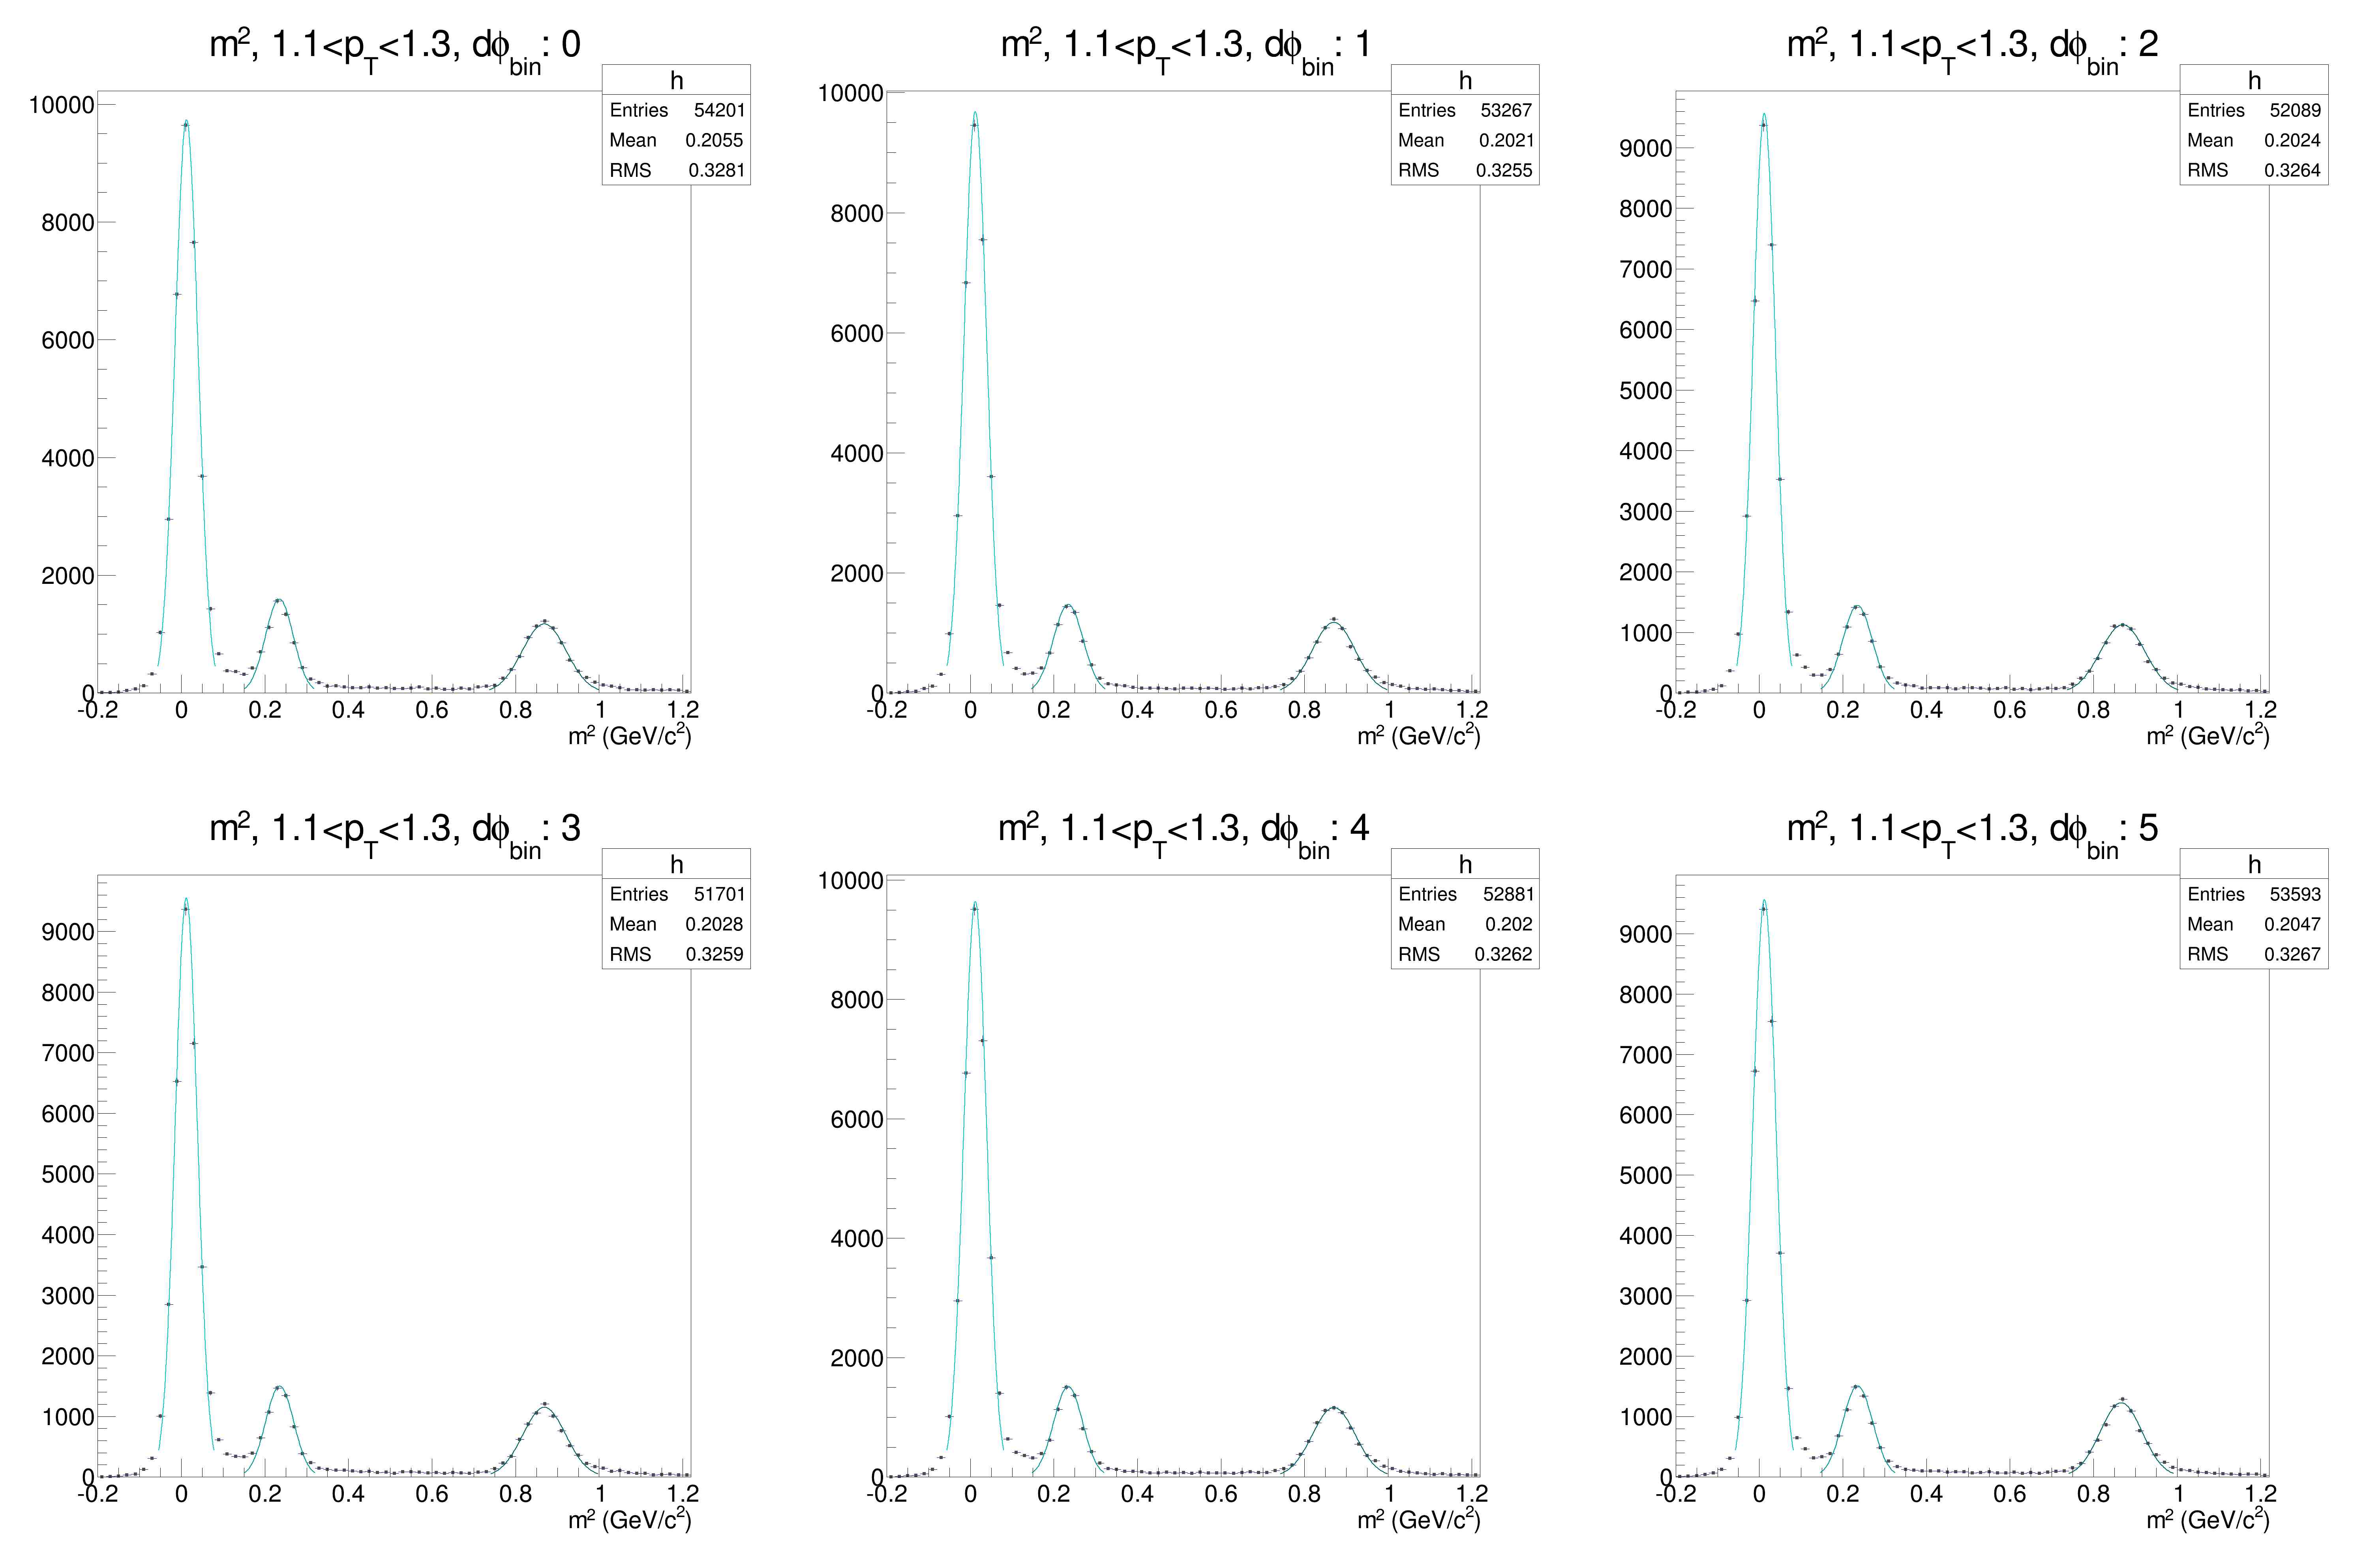
\includegraphics[width=1\textwidth]{lowptfits/yieldvsdphi_tof1_cent0_ch0_pT-11-13.jpg}
    \end{subfigure}
    \begin{subfigure}[p]{1\textwidth}
    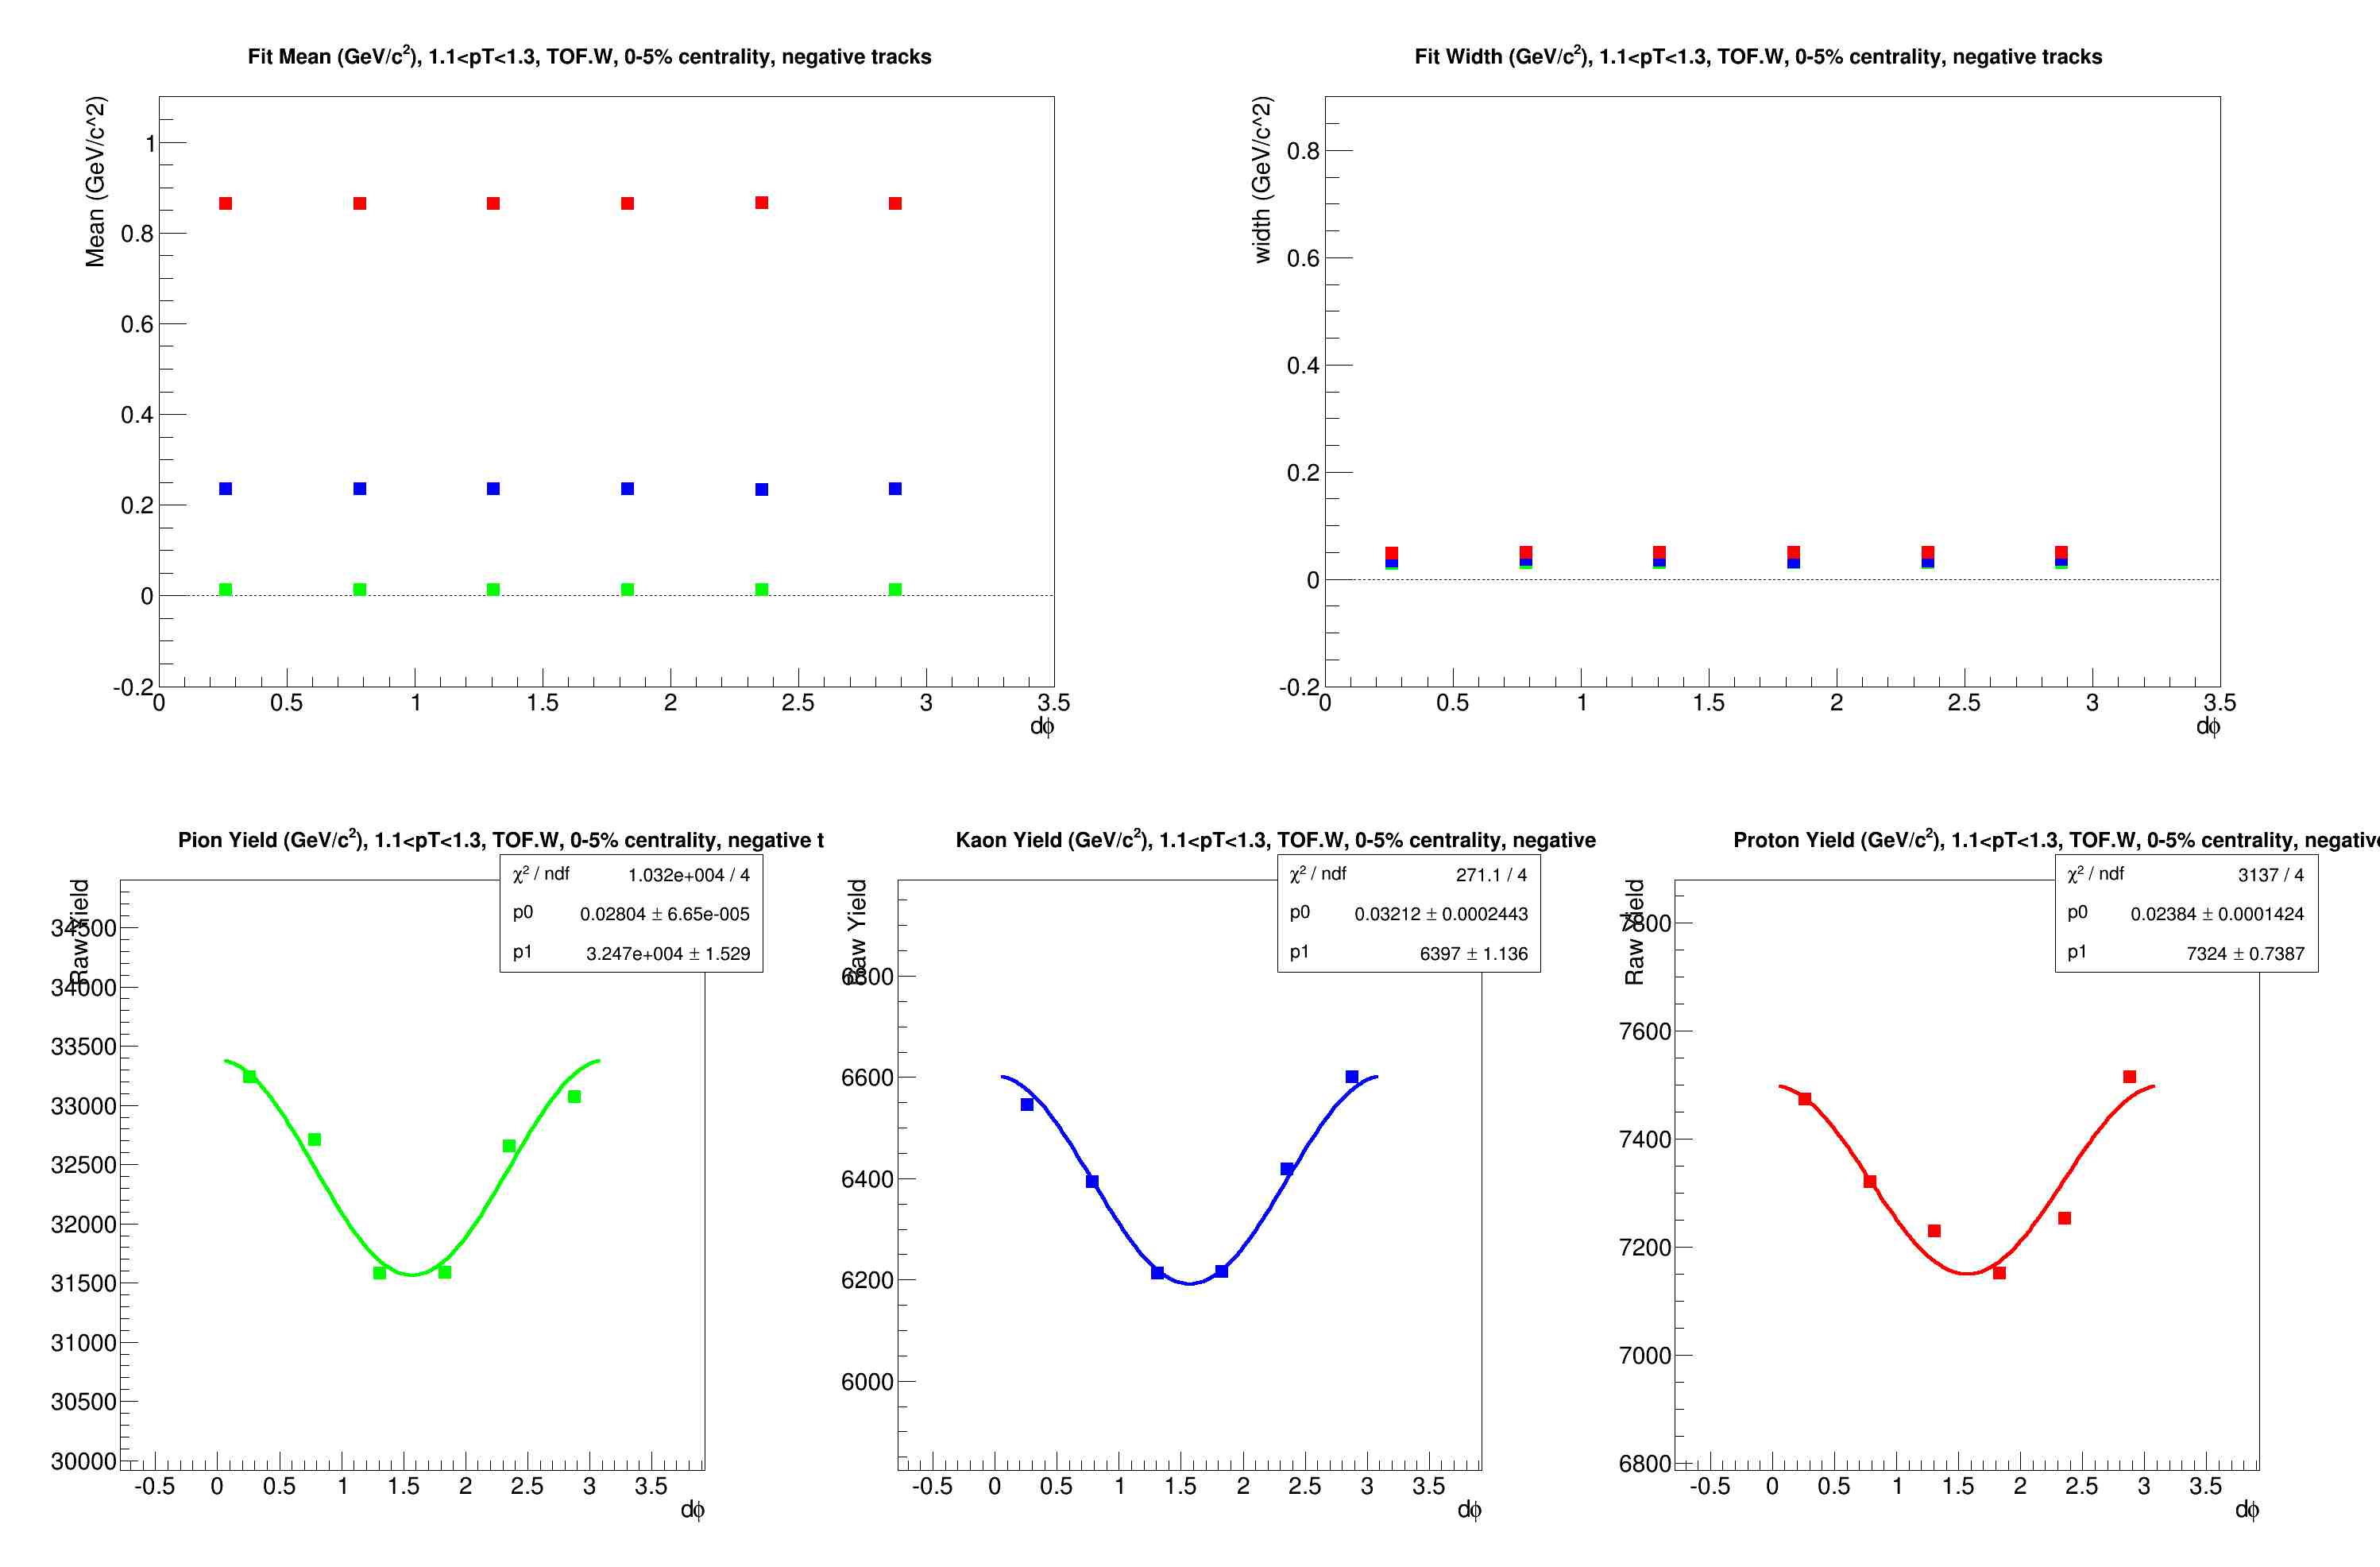
\includegraphics[width=1\textwidth]{lowptfits/fitParams_tof1_cent0_ch0_pT-11-13.jpg}
    \end{subfigure}
    \rule{35em}{0.5pt}
  \caption[PID fits and Yield vs $d\phi$ for $p_T$=1.1-1.3 GeV/c, TOF.W, negative particles ]{$m^2$ Gaussian fits for PID and resulting Yield vs $d\phi$ for $p_T$=1.1-1.3 GeV/c, TOF.W, negative particles}
  \label{fig:fits11-13neg}
\end{figure}

\subsection{Single Gaussian fits, $p_T$=0.5-1.3 GeV/c, TOF.W, positive charged tracks}

\begin{figure}[H]
  \centering
    \begin{subfigure}[p]{1\textwidth}
    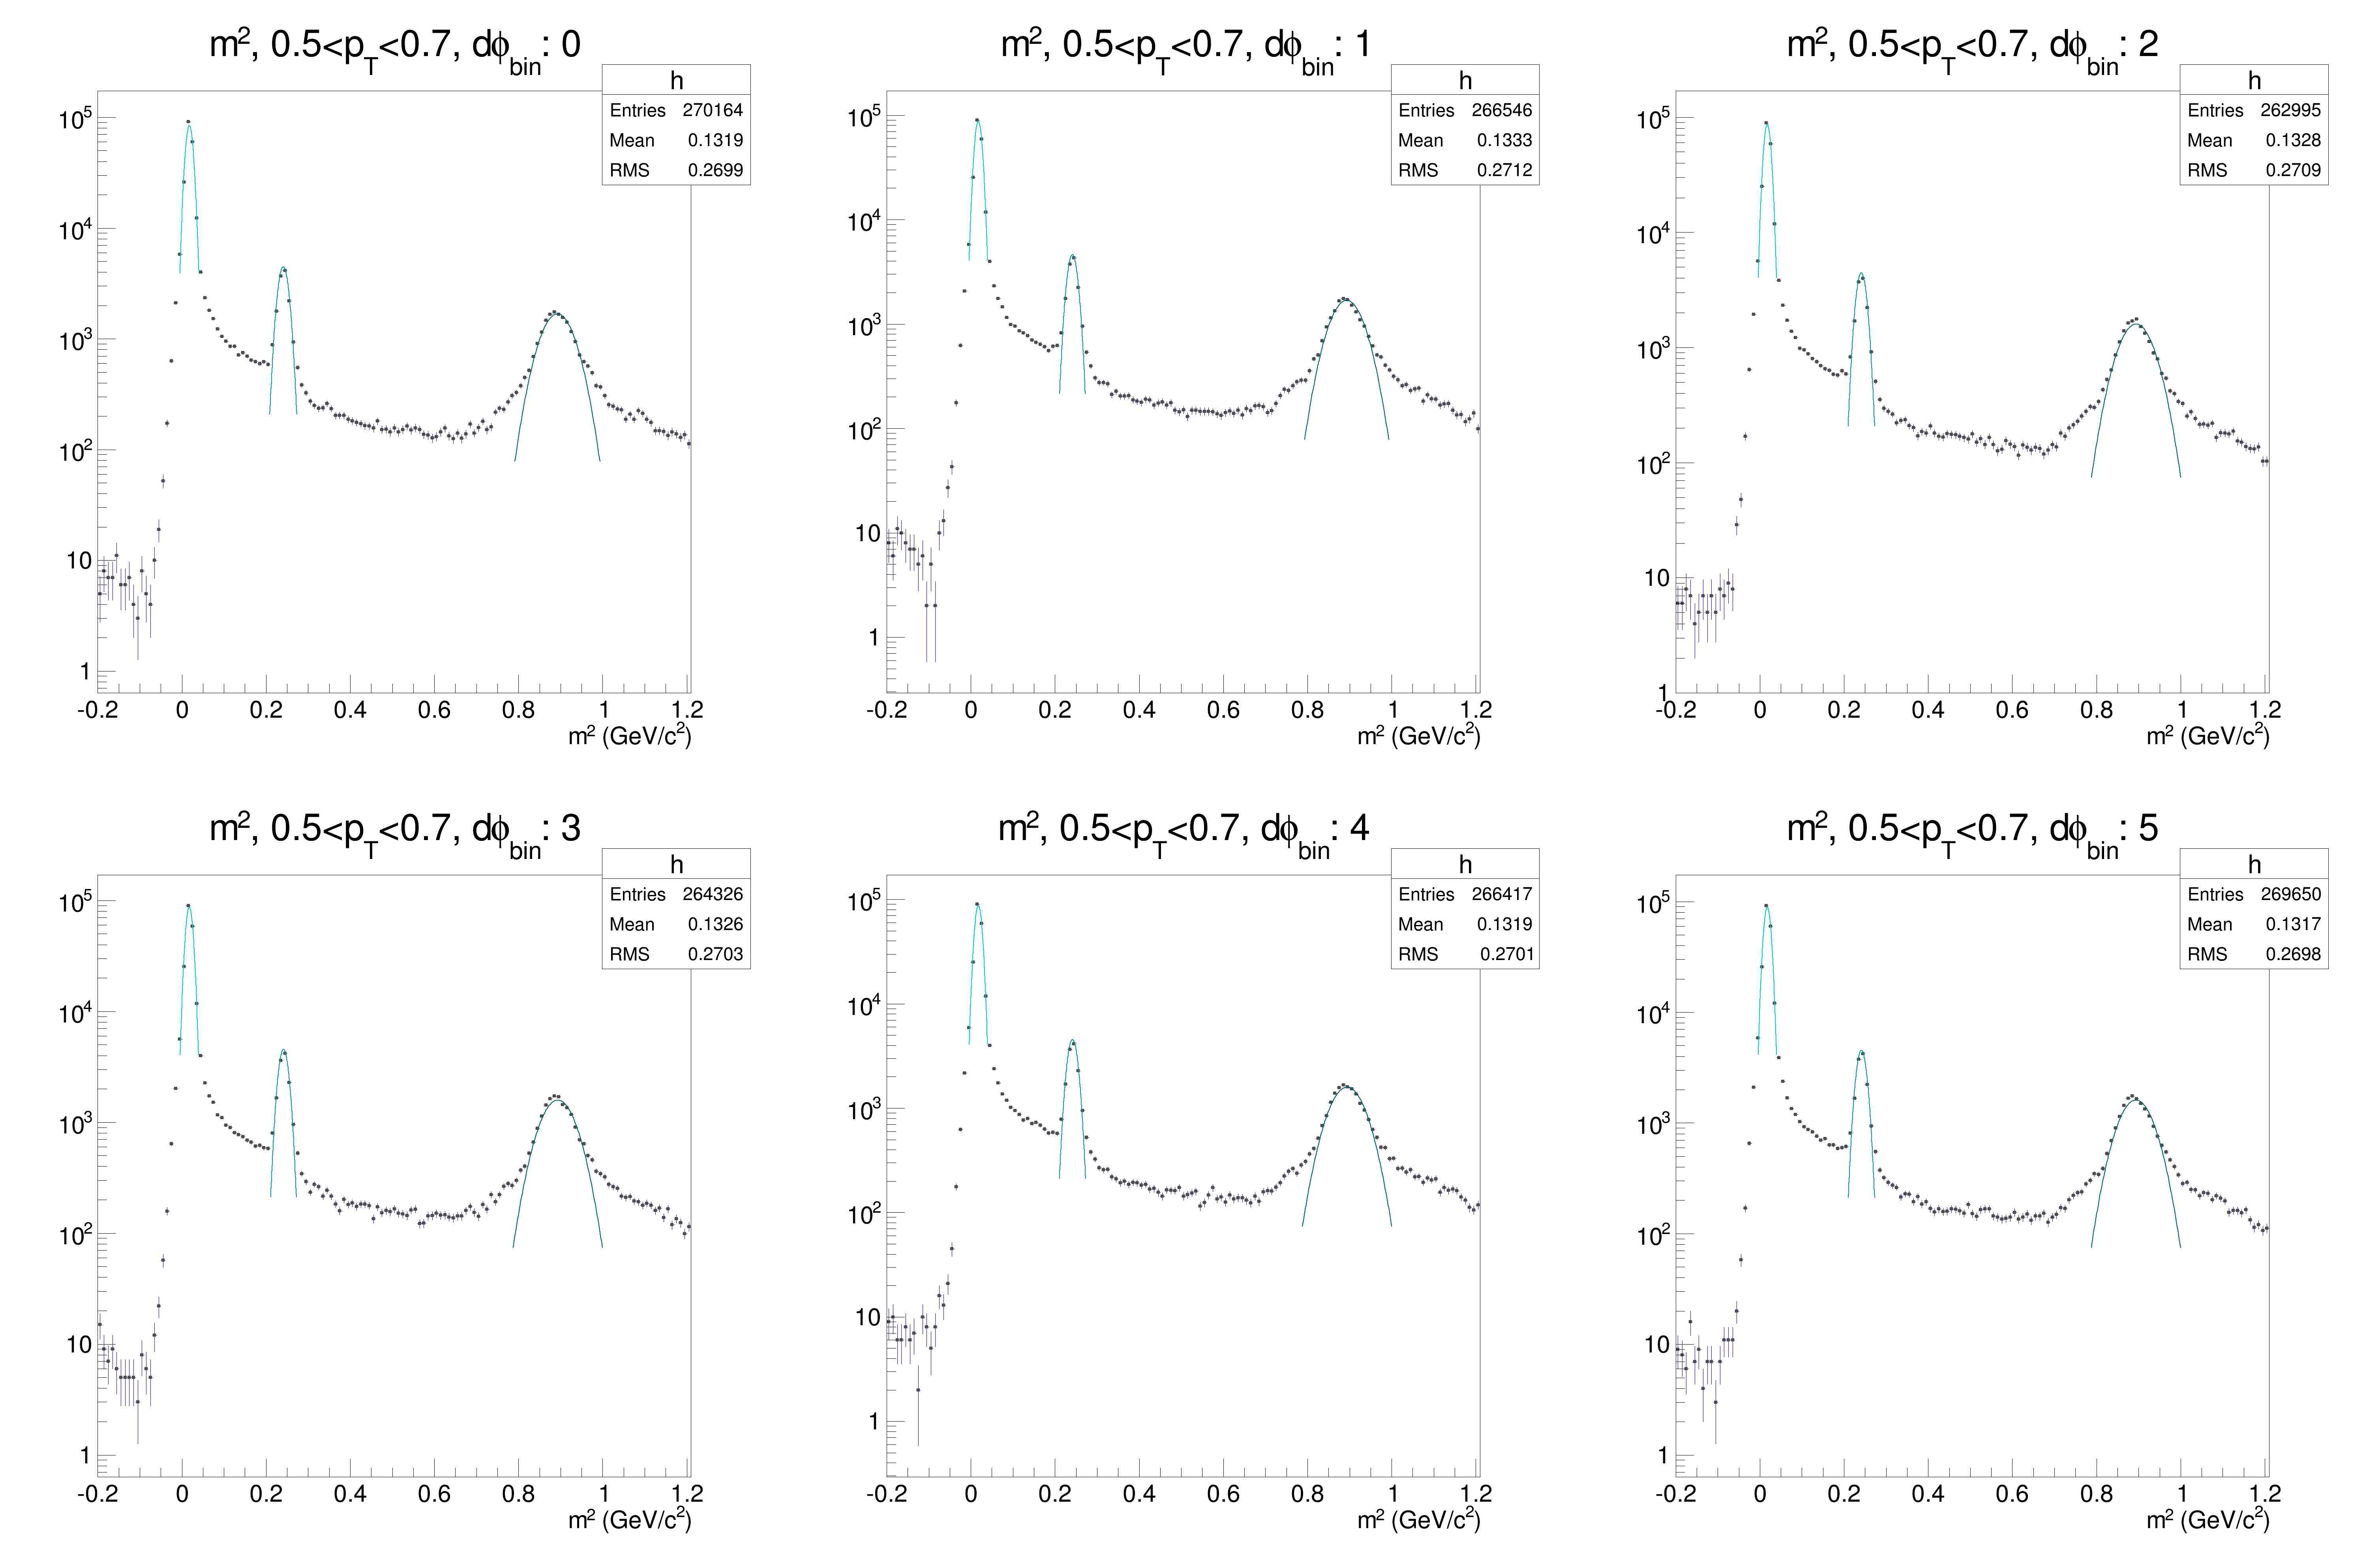
\includegraphics[width=1\textwidth]{lowptfits/yieldvsdphi_tof1_cent0_ch1_pT-5-7.jpg}
    \end{subfigure}
    \begin{subfigure}[p]{1\textwidth}
    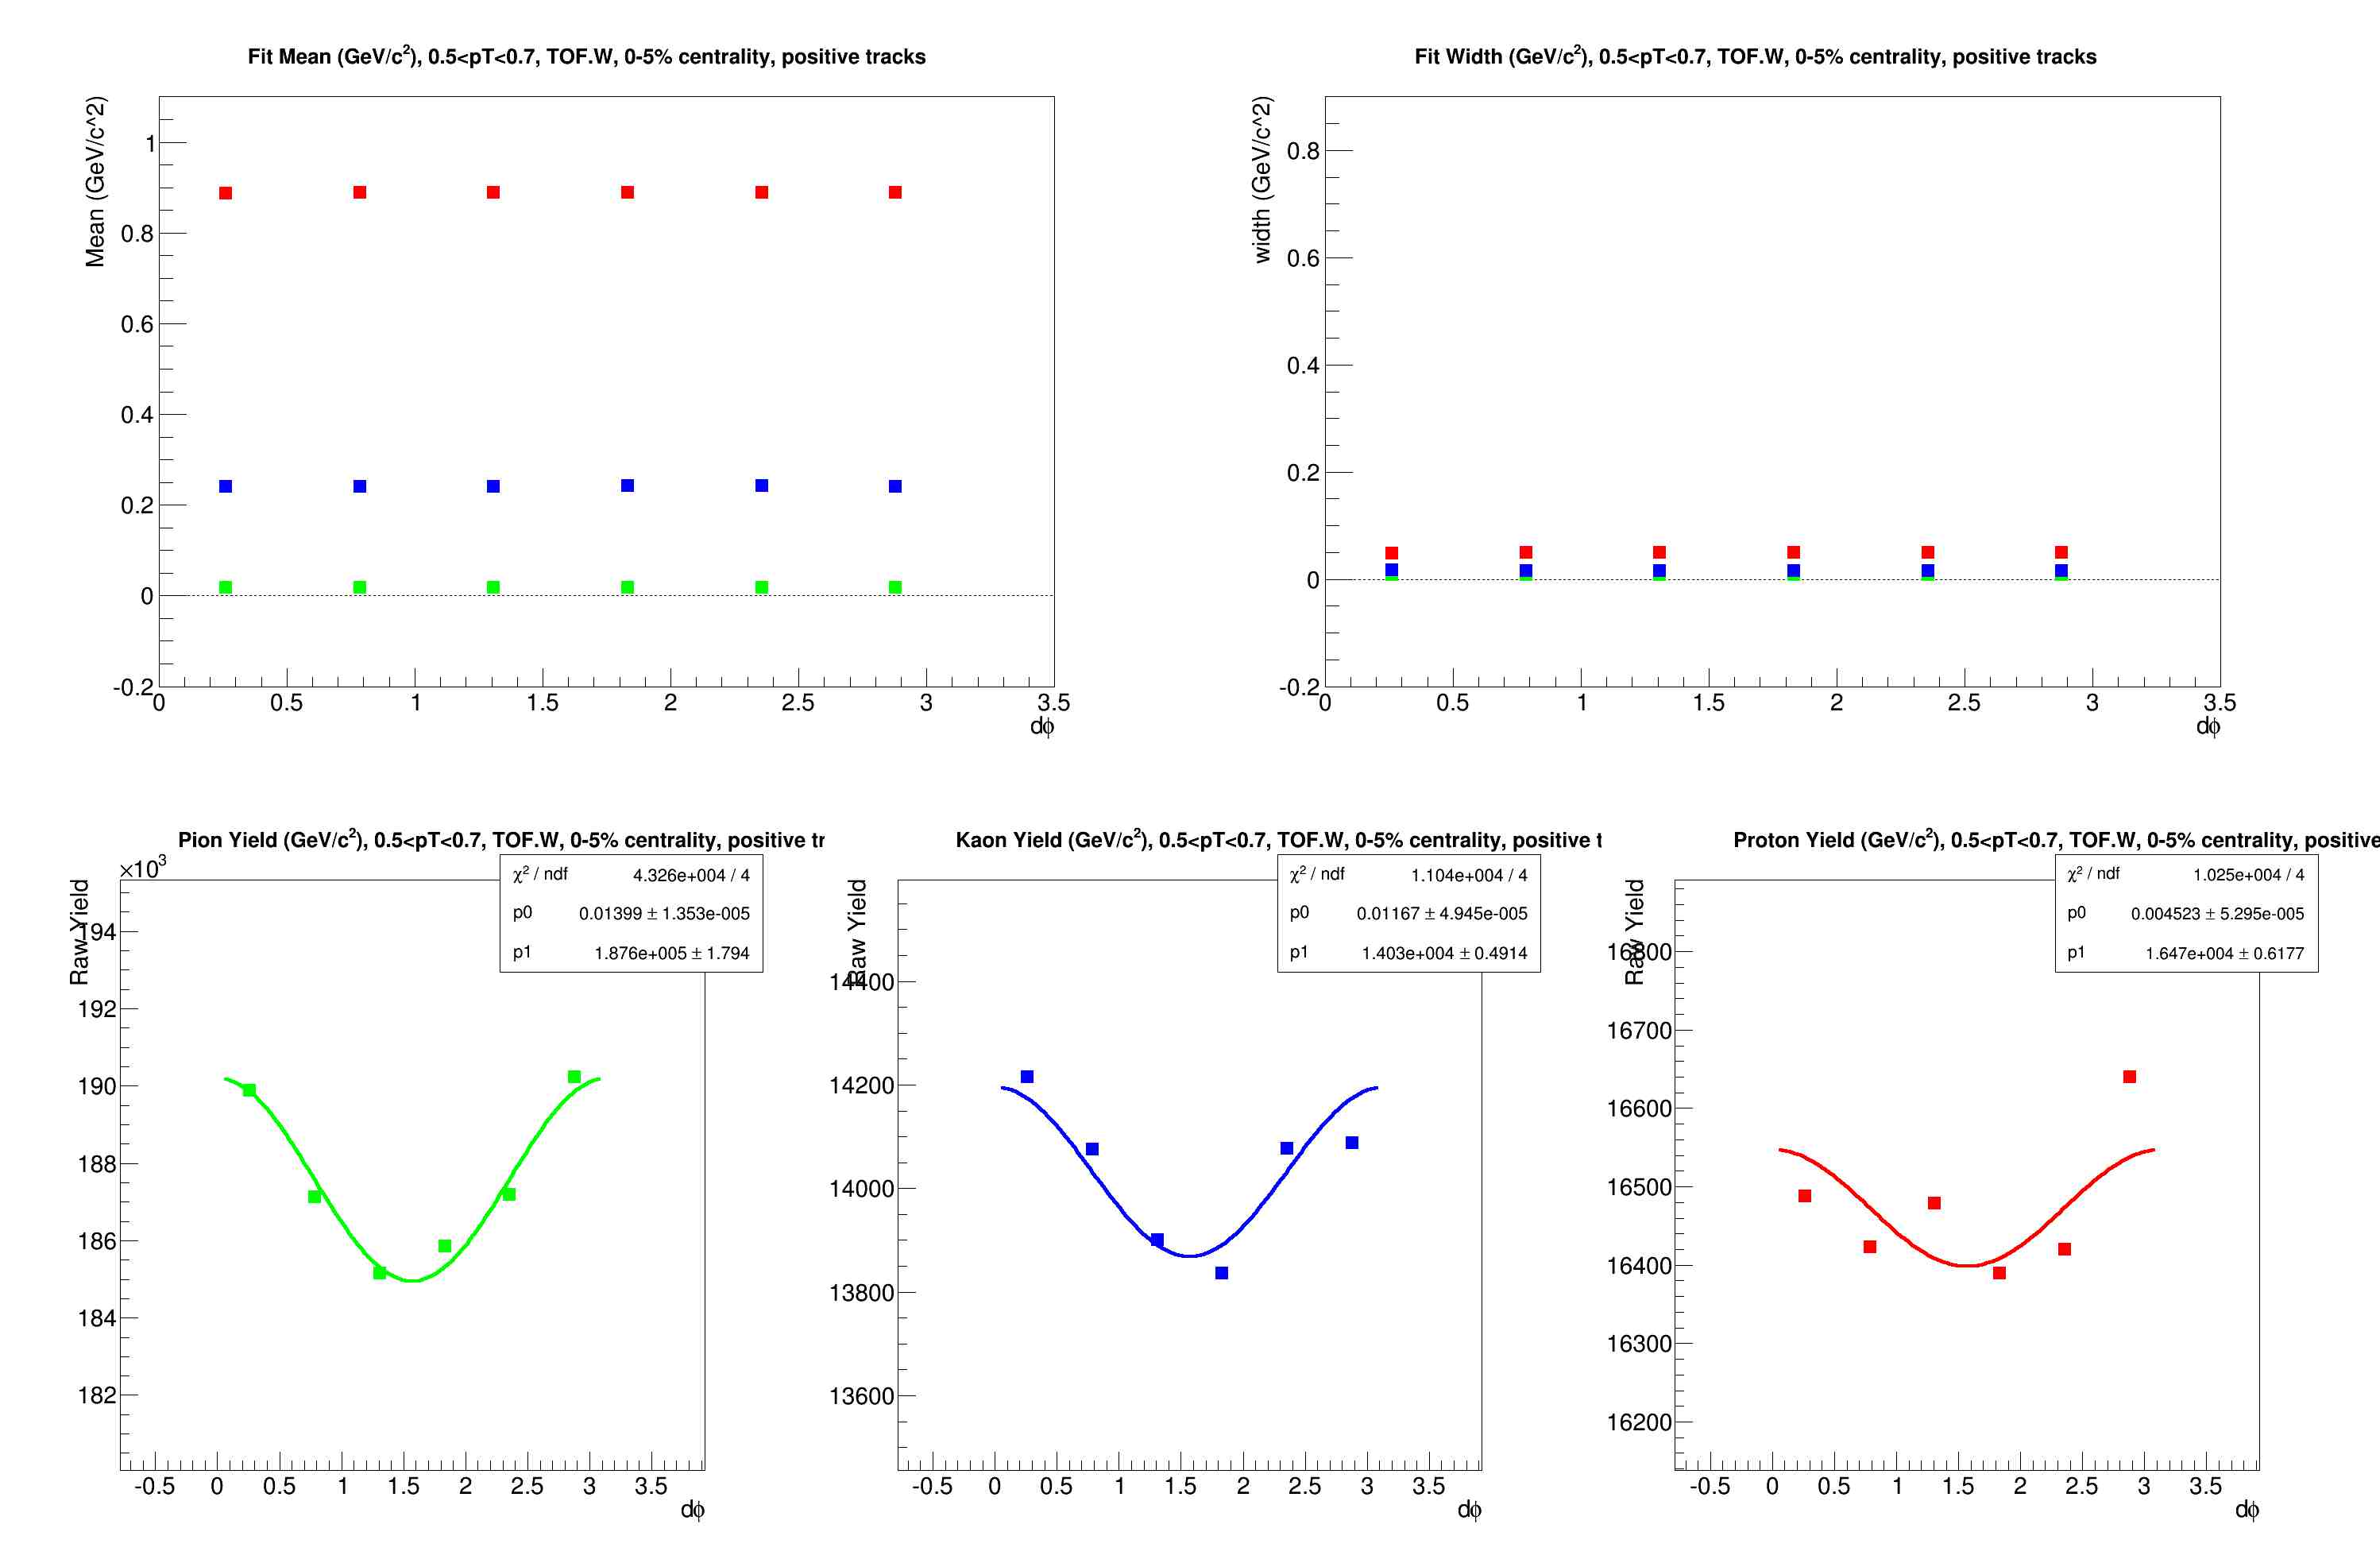
\includegraphics[width=1\textwidth]{lowptfits/fitParams_tof1_cent0_ch1_pT-5-7.jpg}
    \end{subfigure}
    \rule{35em}{0.5pt}
  \caption[PID fits and Yield vs $d\phi$ for $p_T$=0.5-0.7 GeV/c, TOF.W, positive particles ]{$m^2$ Gaussian fits for PID and resulting Yield vs $d\phi$ for $p_T$=0.5-0.7 GeV/c, TOF.W, positive particles}
  \label{fig:fits5-7pos}
\end{figure}

\begin{figure}[H]
  \centering
    \begin{subfigure}[p]{1\textwidth}
    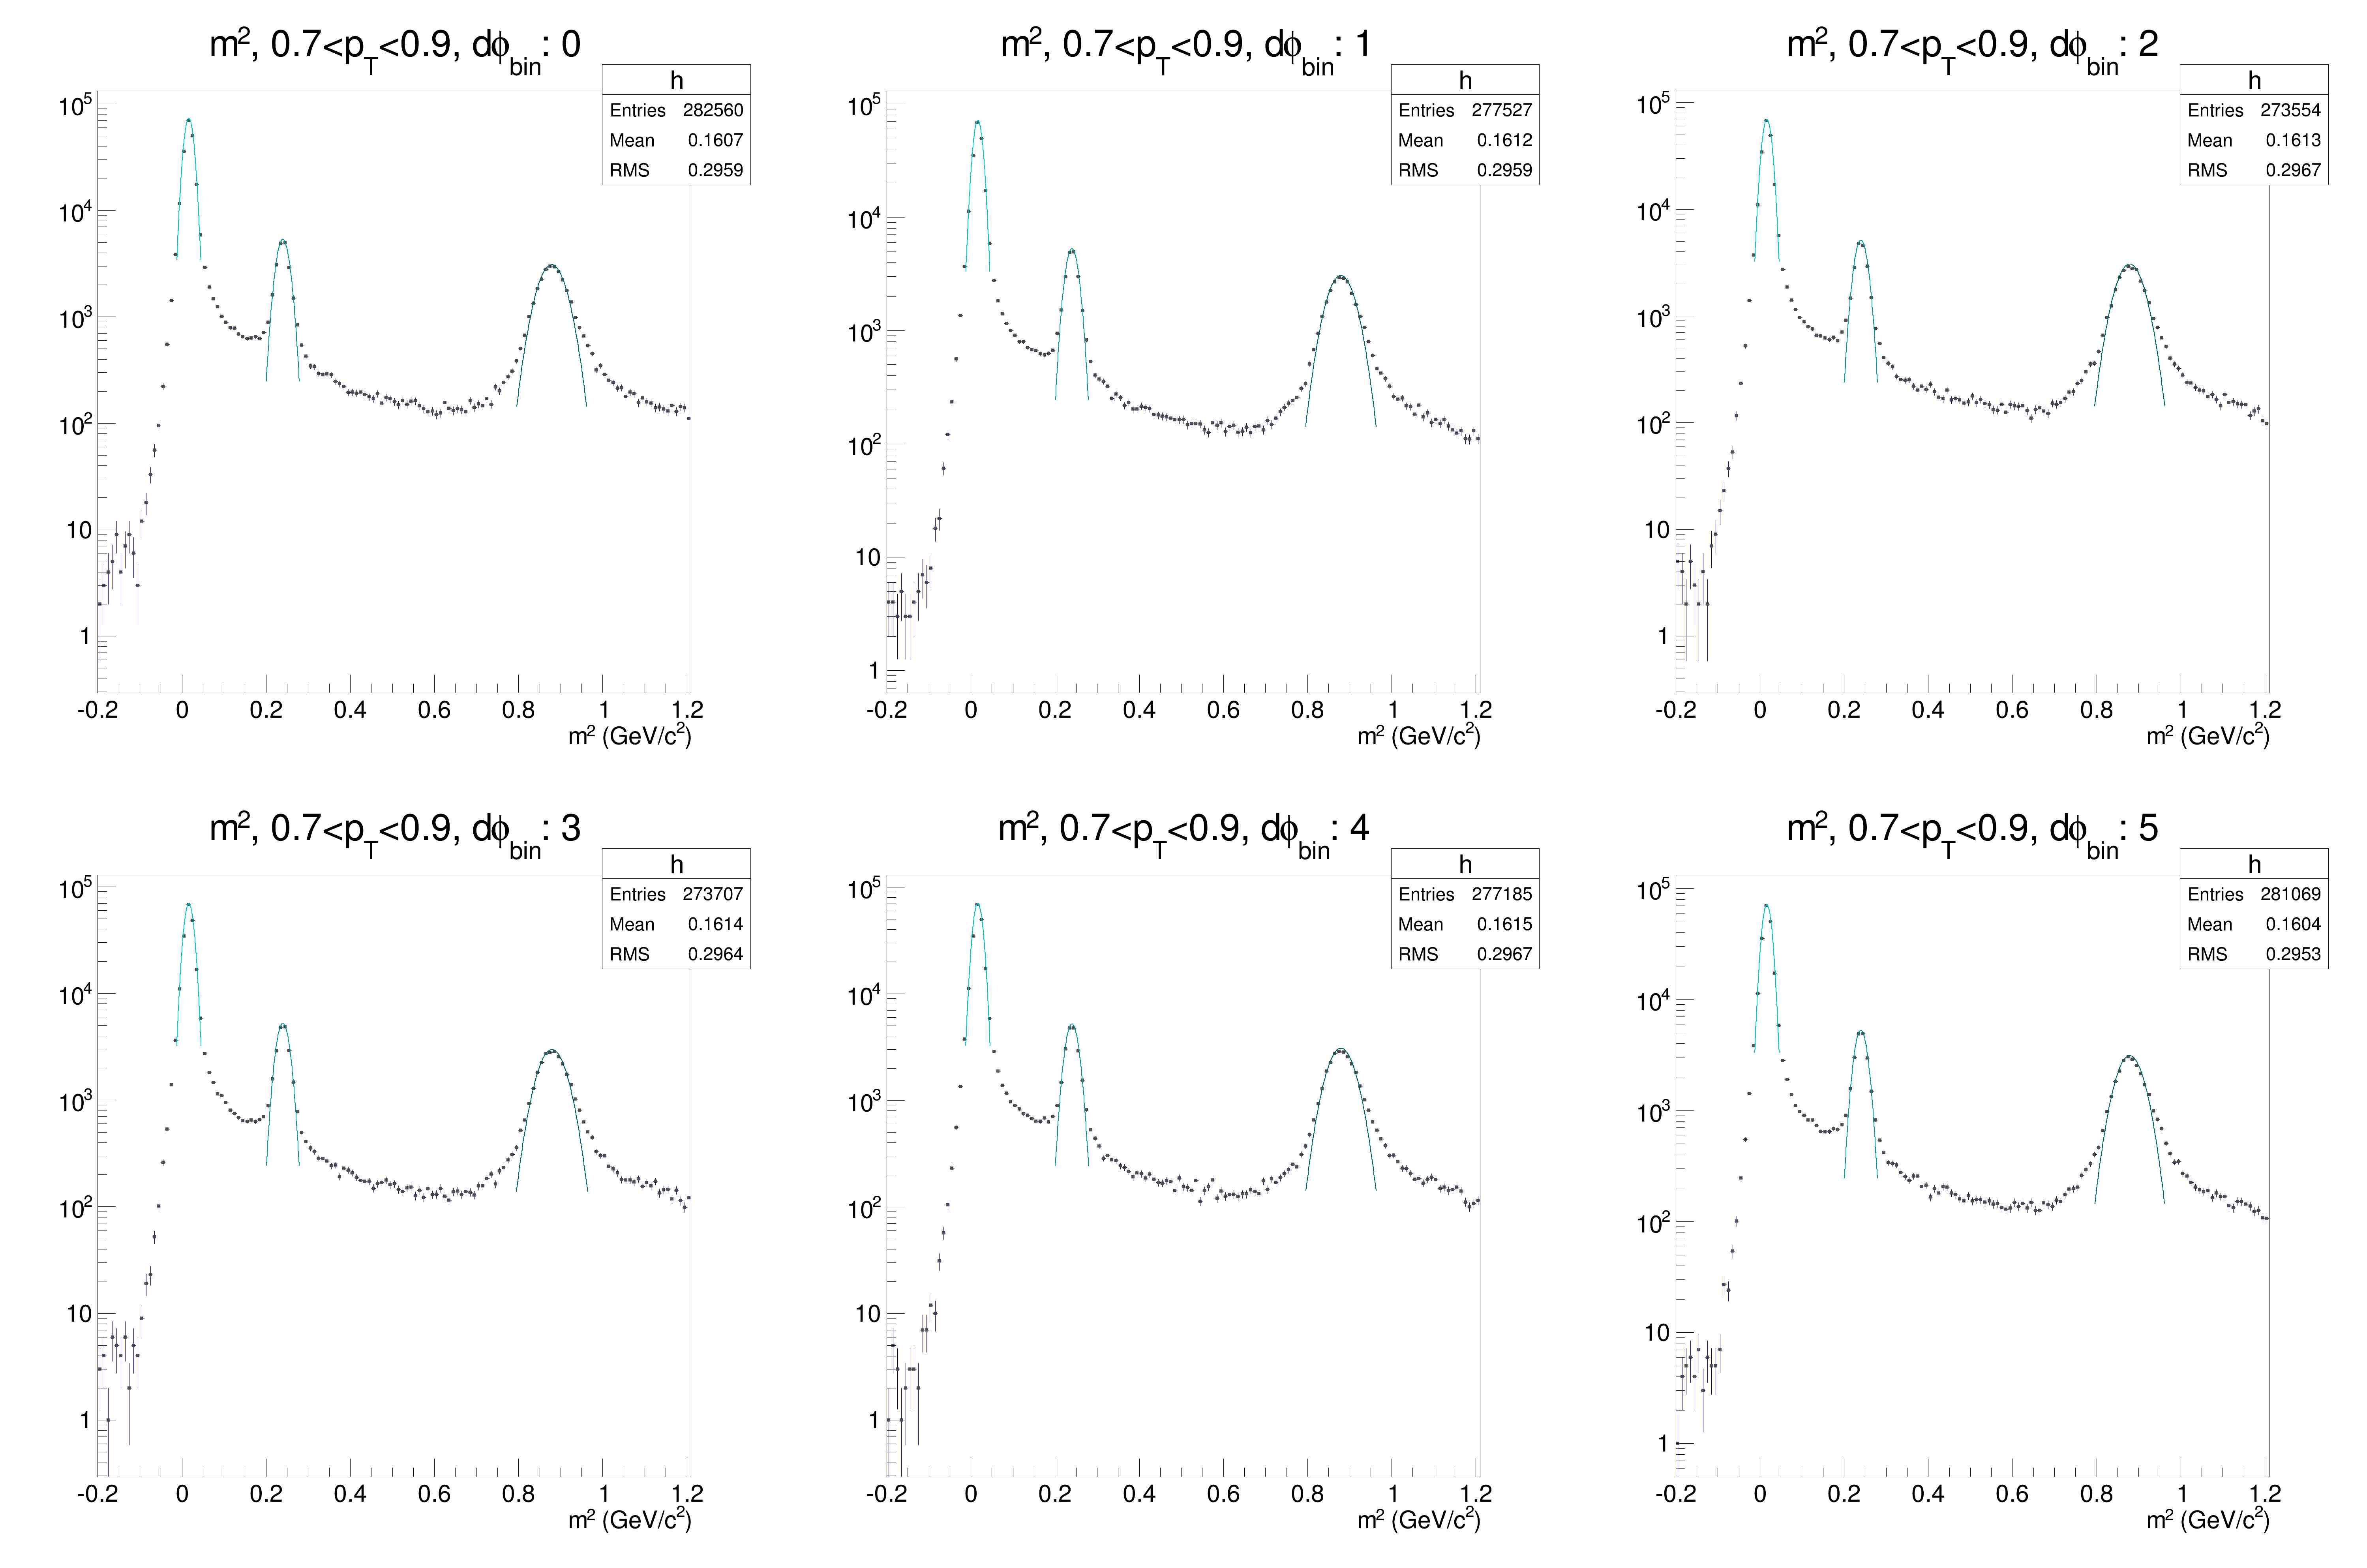
\includegraphics[width=1\textwidth]{lowptfits/yieldvsdphi_tof1_cent0_ch1_pT-7-9.jpg}
    \end{subfigure}
    \begin{subfigure}[p]{1\textwidth}
    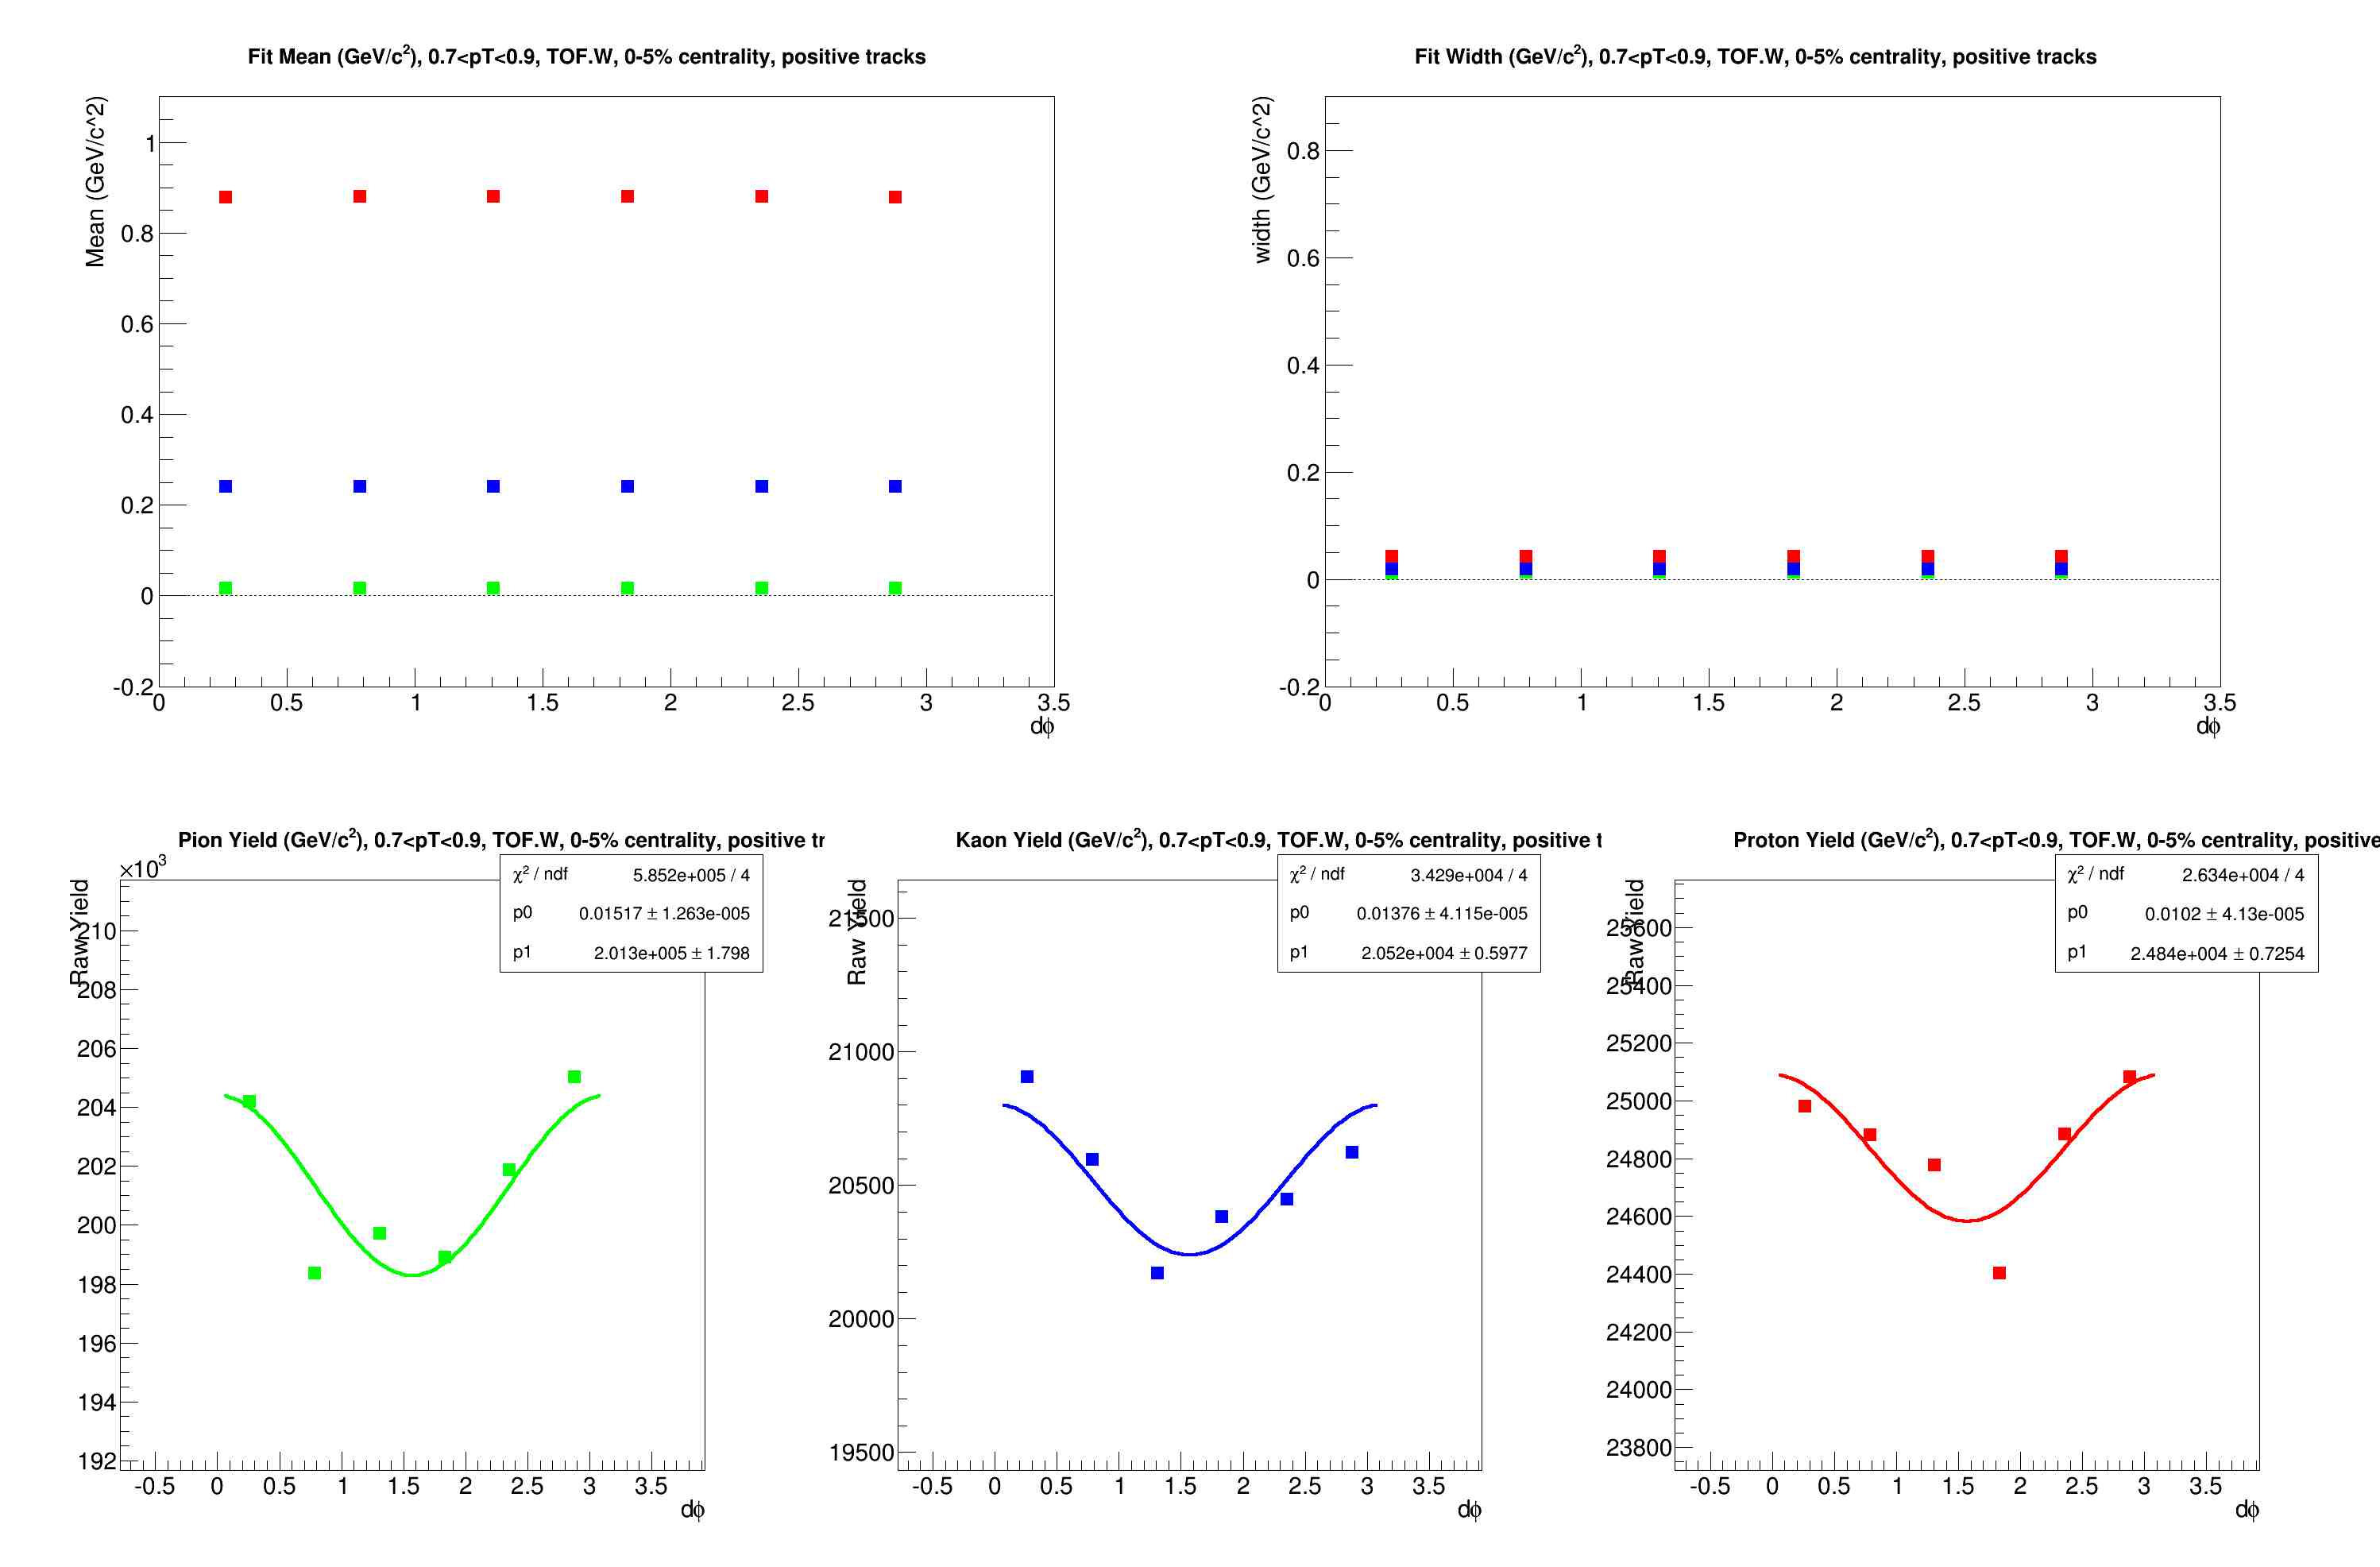
\includegraphics[width=1\textwidth]{lowptfits/fitParams_tof1_cent0_ch1_pT-7-9.jpg}
    \end{subfigure}
    \rule{35em}{0.5pt}
  \caption[PID fits and Yield vs $d\phi$ for $p_T$=0.7-0.9 GeV/c, TOF.W, positive particles ]{$m^2$ Gaussian fits for PID and resulting Yield vs $d\phi$ for $p_T$=0.7-0.9 GeV/c, TOF.W, positive particles}
  \label{fig:fits7-9pos}
\end{figure}

\begin{figure}[H]
  \centering
    \begin{subfigure}[p]{1\textwidth}
    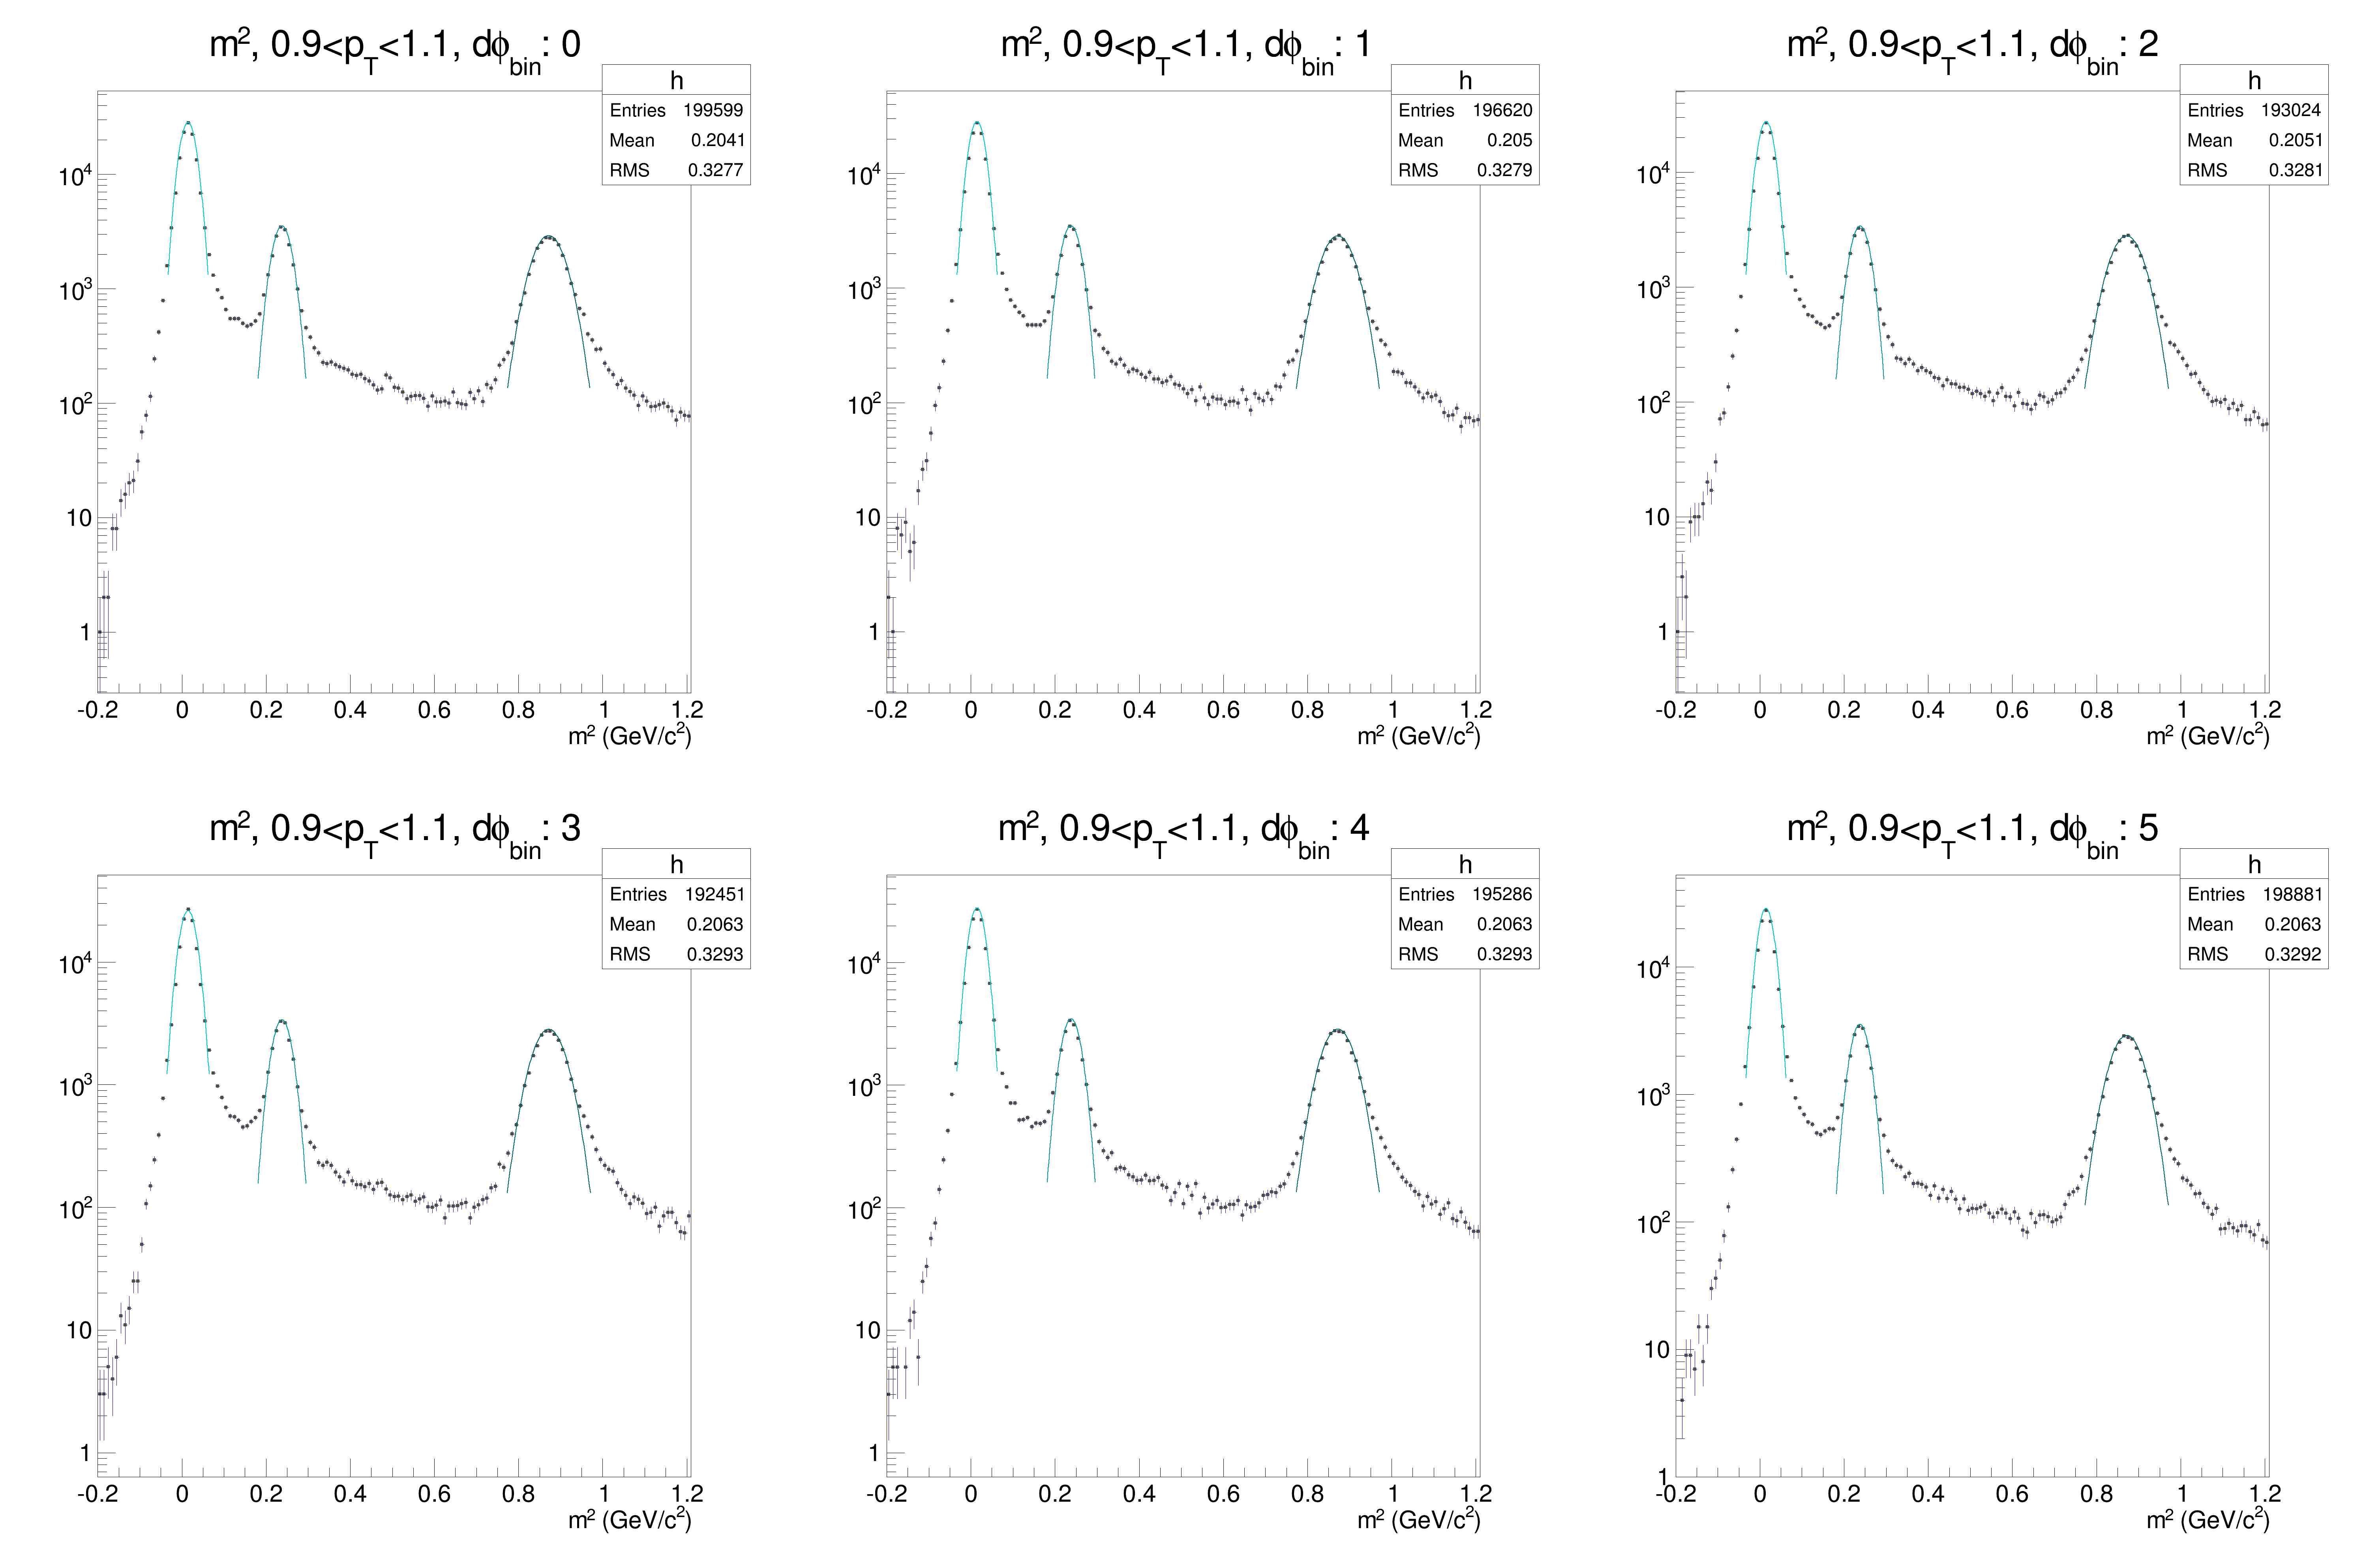
\includegraphics[width=1\textwidth]{lowptfits/yieldvsdphi_tof1_cent0_ch1_pT-9-11.jpg}
    \end{subfigure}
    \begin{subfigure}[p]{1\textwidth}
    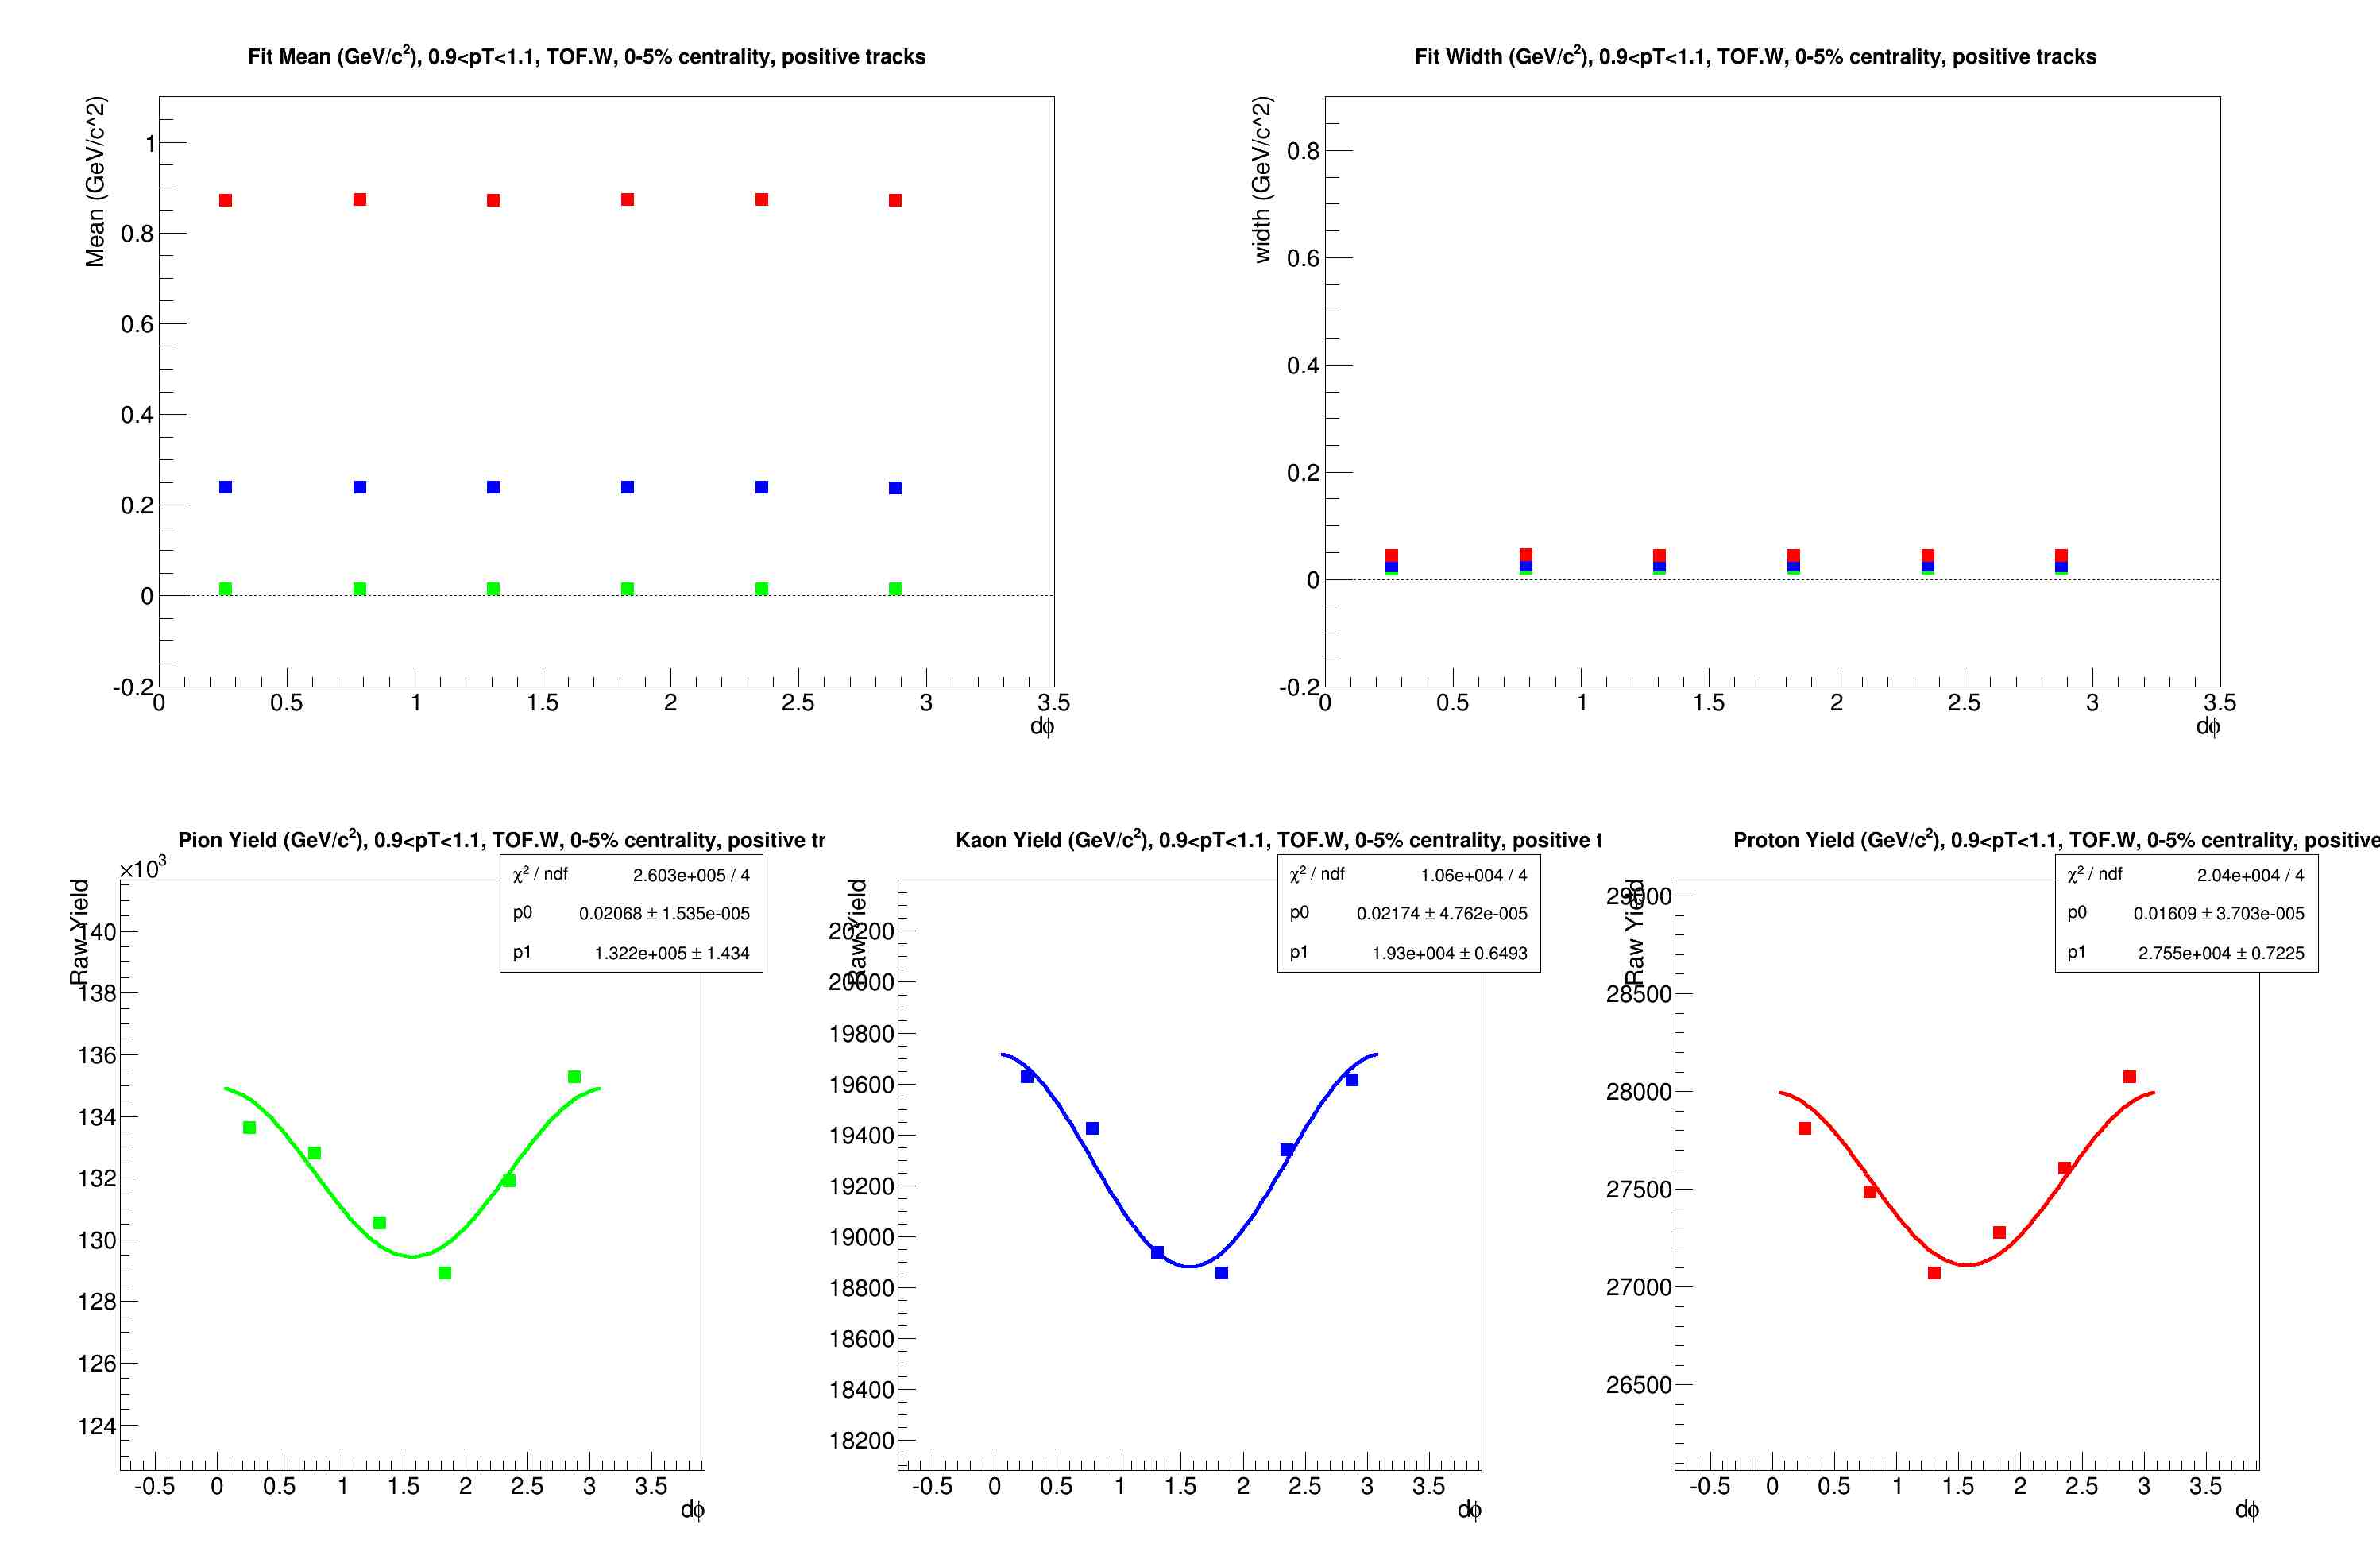
\includegraphics[width=1\textwidth]{lowptfits/fitParams_tof1_cent0_ch1_pT-9-11.jpg}
    \end{subfigure}
    \rule{35em}{0.5pt}
  \caption[PID fits and Yield vs $d\phi$ for $p_T$=0.9-1.1 GeV/c, TOF.W, positive particles ]{$m^2$ Gaussian fits for PID and resulting Yield vs $d\phi$ for $p_T$=0.9-1.1 GeV/c, TOF.W, positive particles}
  \label{fig:fits9-11pos}
\end{figure}

\begin{figure}[H]
  \centering
    \begin{subfigure}[p]{1\textwidth}
    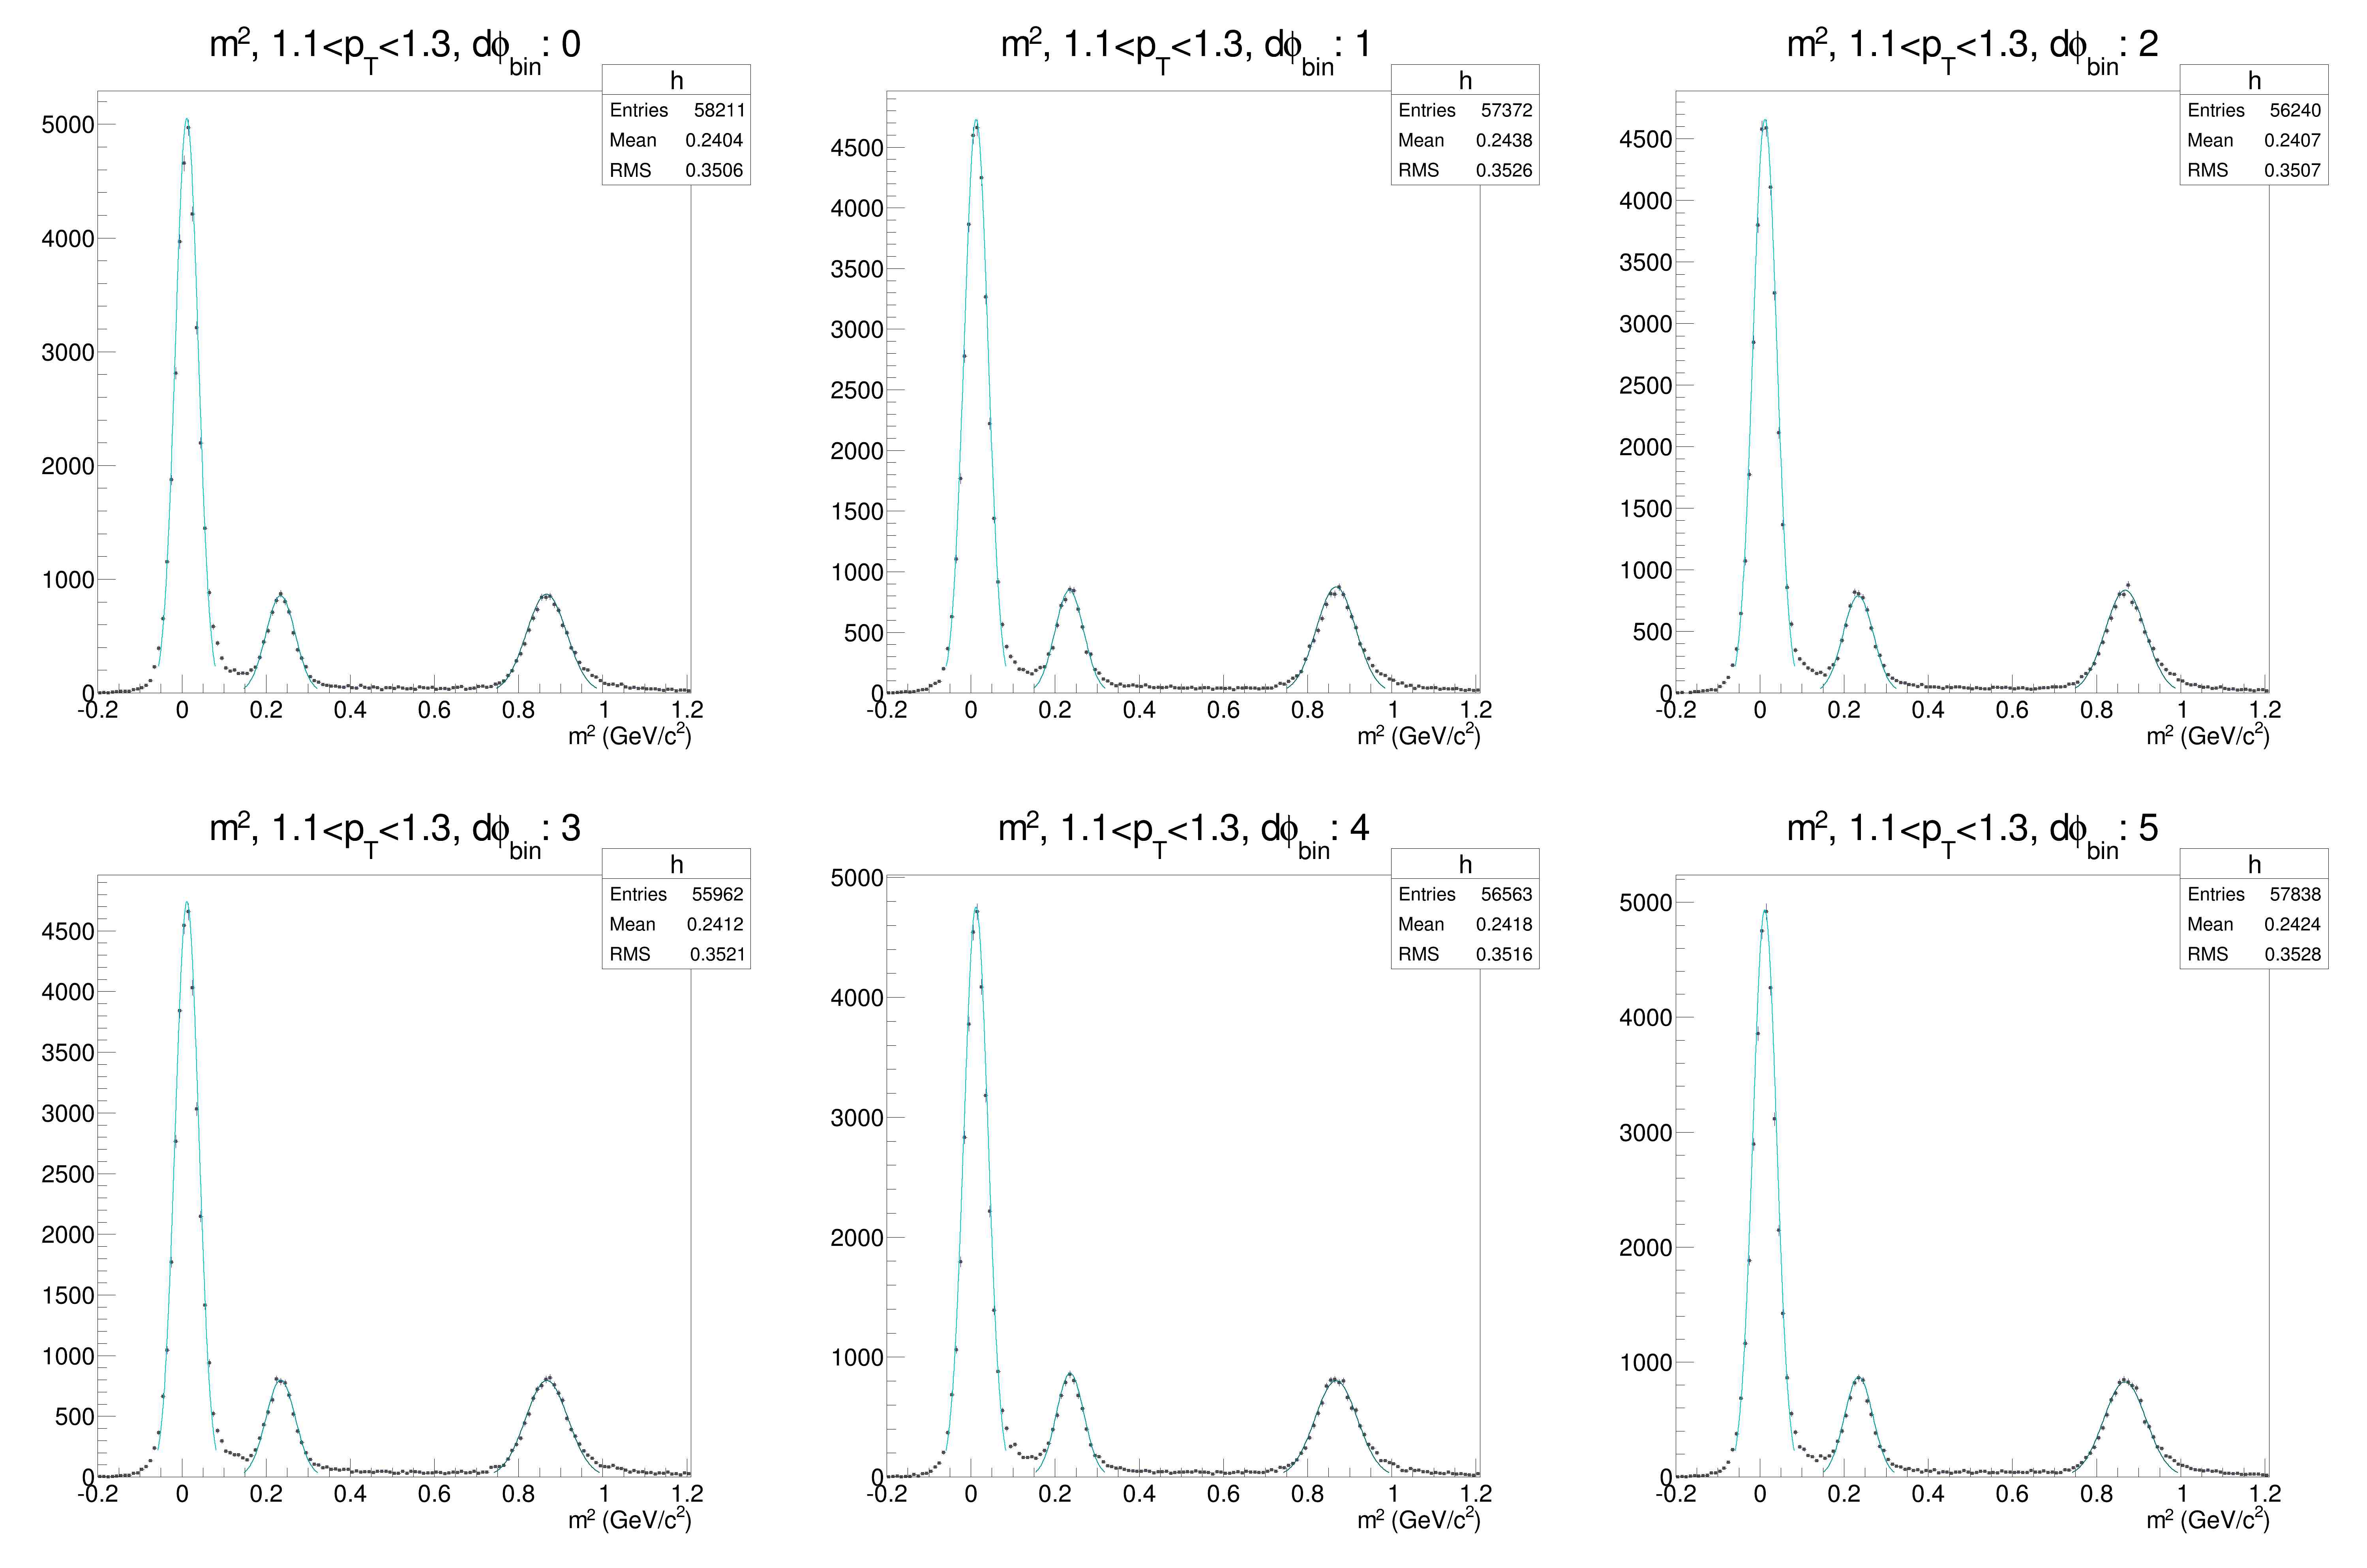
\includegraphics[width=1\textwidth]{lowptfits/yieldvsdphi_tof1_cent0_ch1_pT-11-13.jpg}
    \end{subfigure}
    \begin{subfigure}[p]{1\textwidth}
    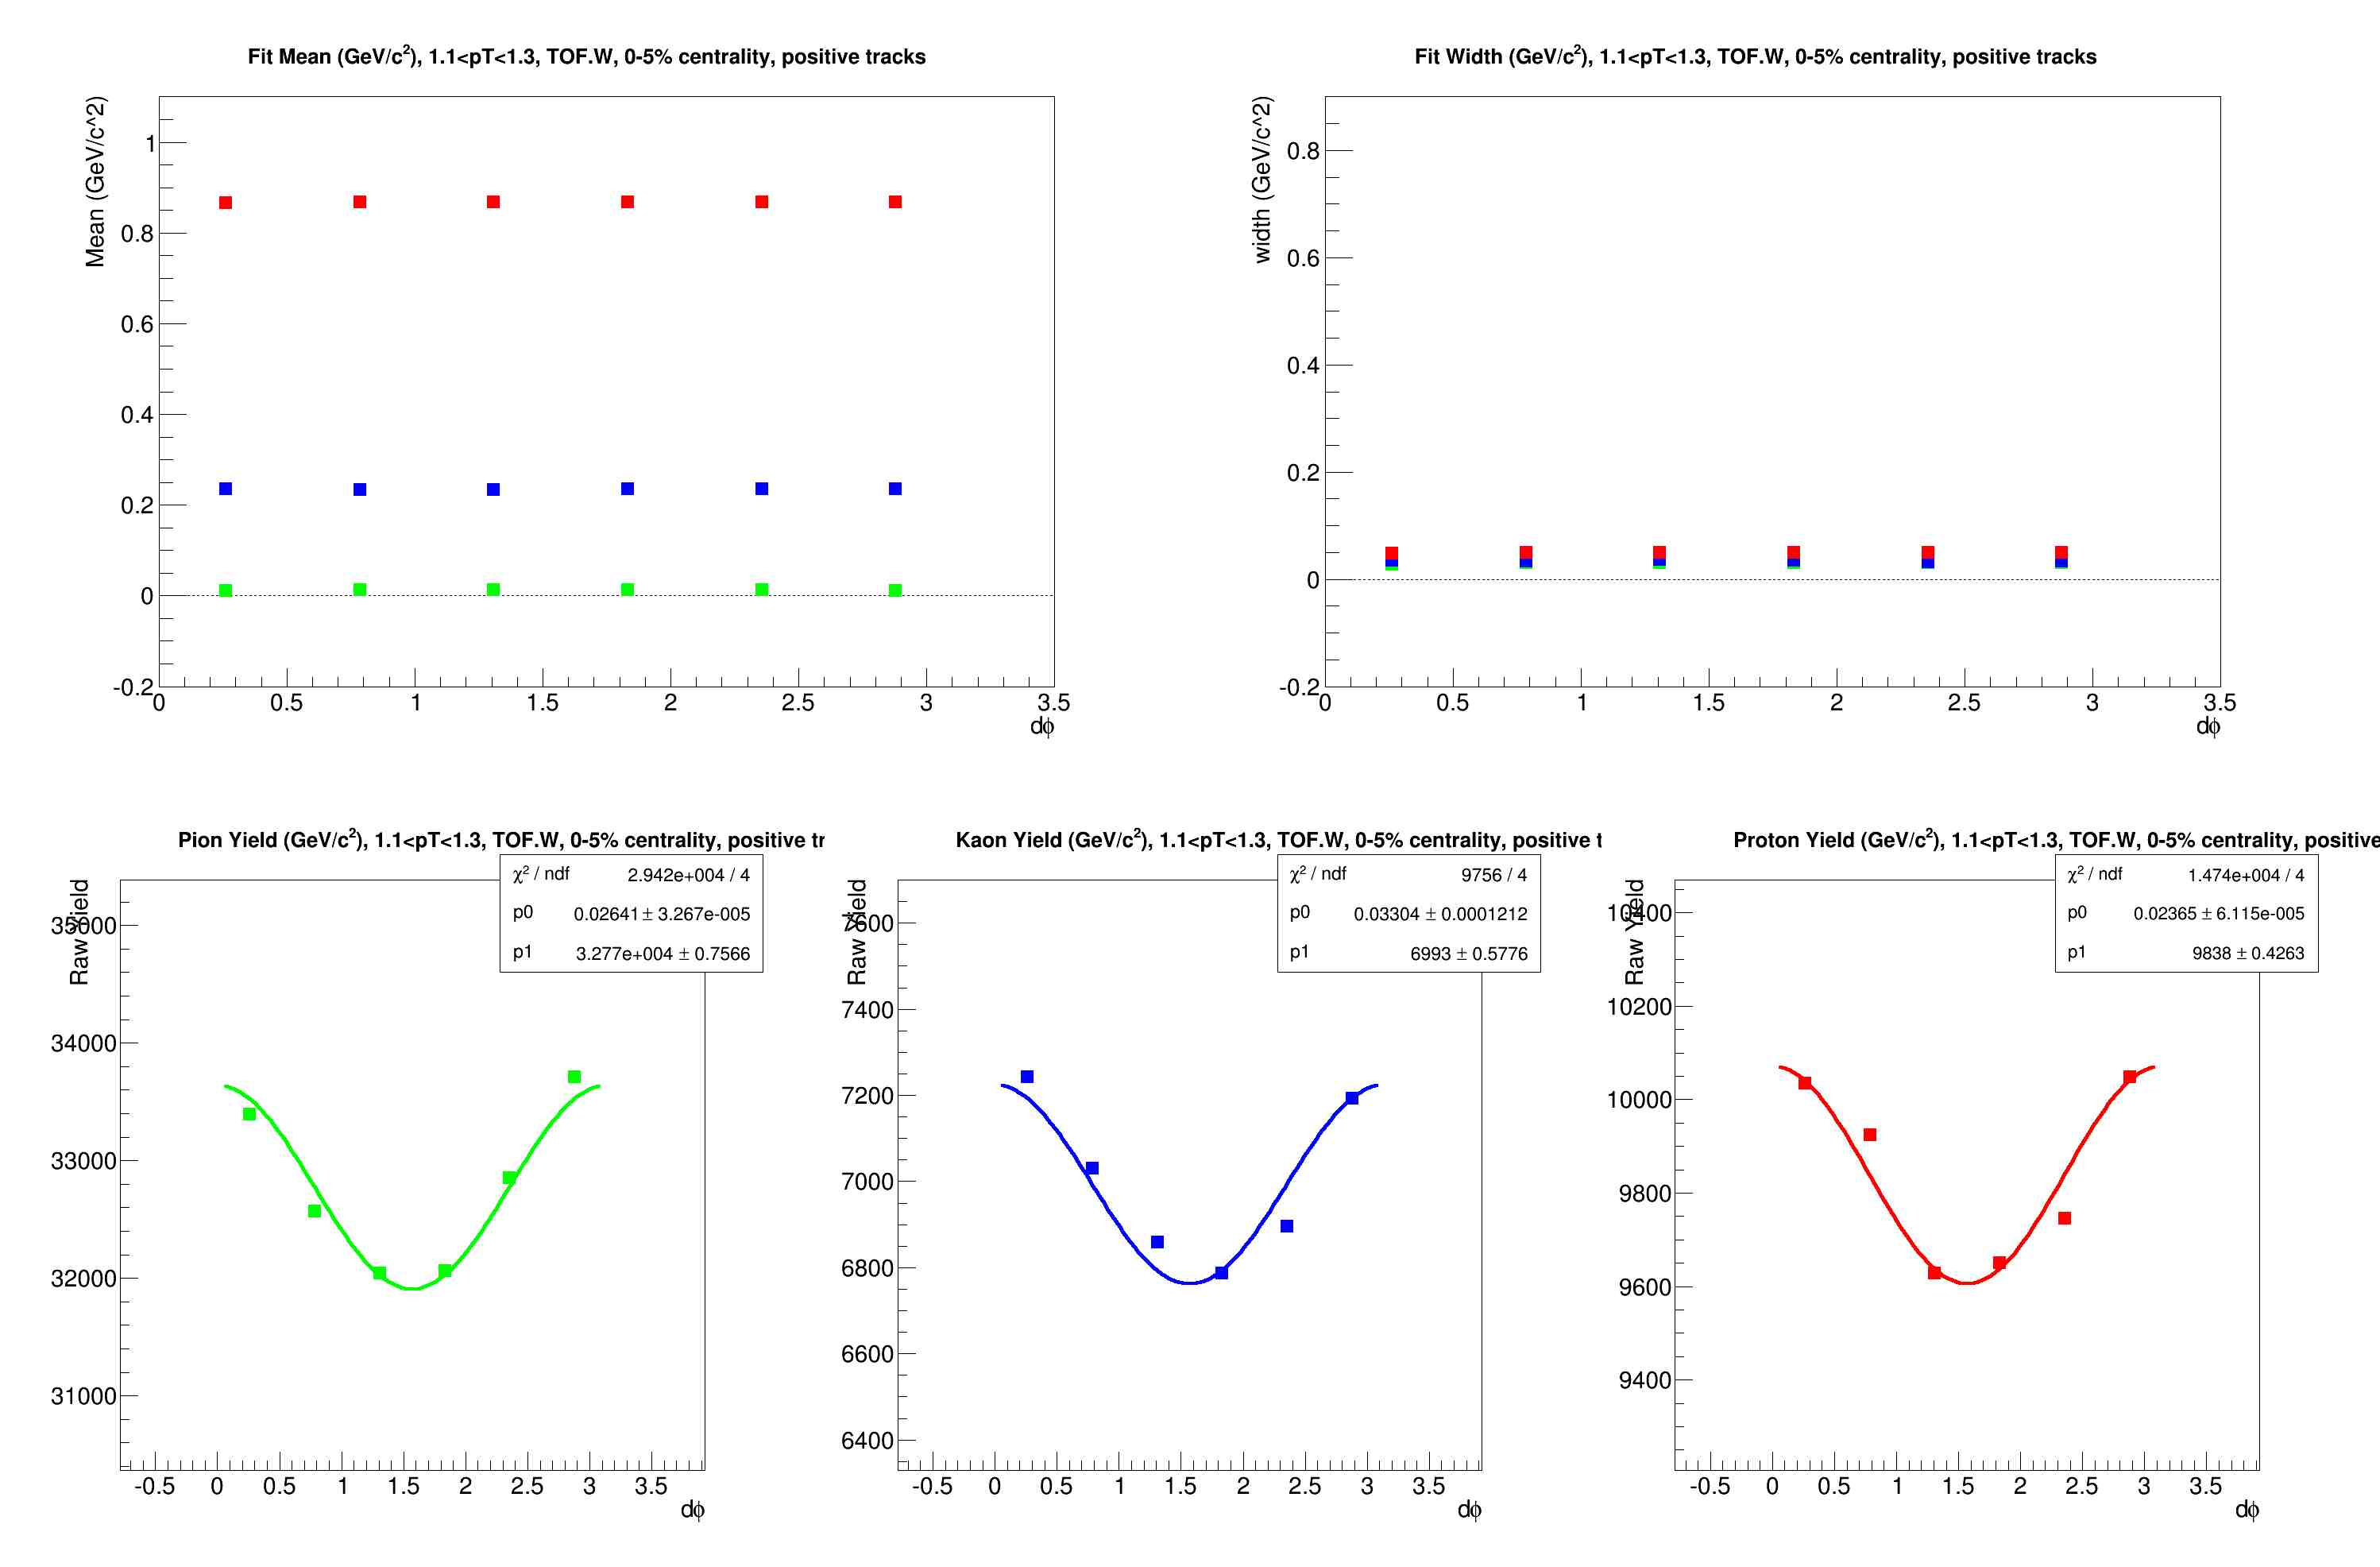
\includegraphics[width=1\textwidth]{lowptfits/fitParams_tof1_cent0_ch1_pT-11-13.jpg}
    \end{subfigure}
    \rule{35em}{0.5pt}
  \caption[PID fits and Yield vs $d\phi$ for $p_T$=1.1-1.3 GeV/c, TOF.W, positive particles ]{$m^2$ Gaussian fits for PID and resulting Yield vs $d\phi$ for $p_T$=1.1-1.3 GeV/c, TOF.W, positive particles}
  \label{fig:fits11-13pos}
\end{figure}


\subsection{Mixed Gaussian fits, $p_T$=1.3-2.1 GeV/c, TOF.W, negative charged tracks}
\label{app:mixgauss}
\begin{figure}[H]
  \centering
    \begin{subfigure}{1\textwidth}
    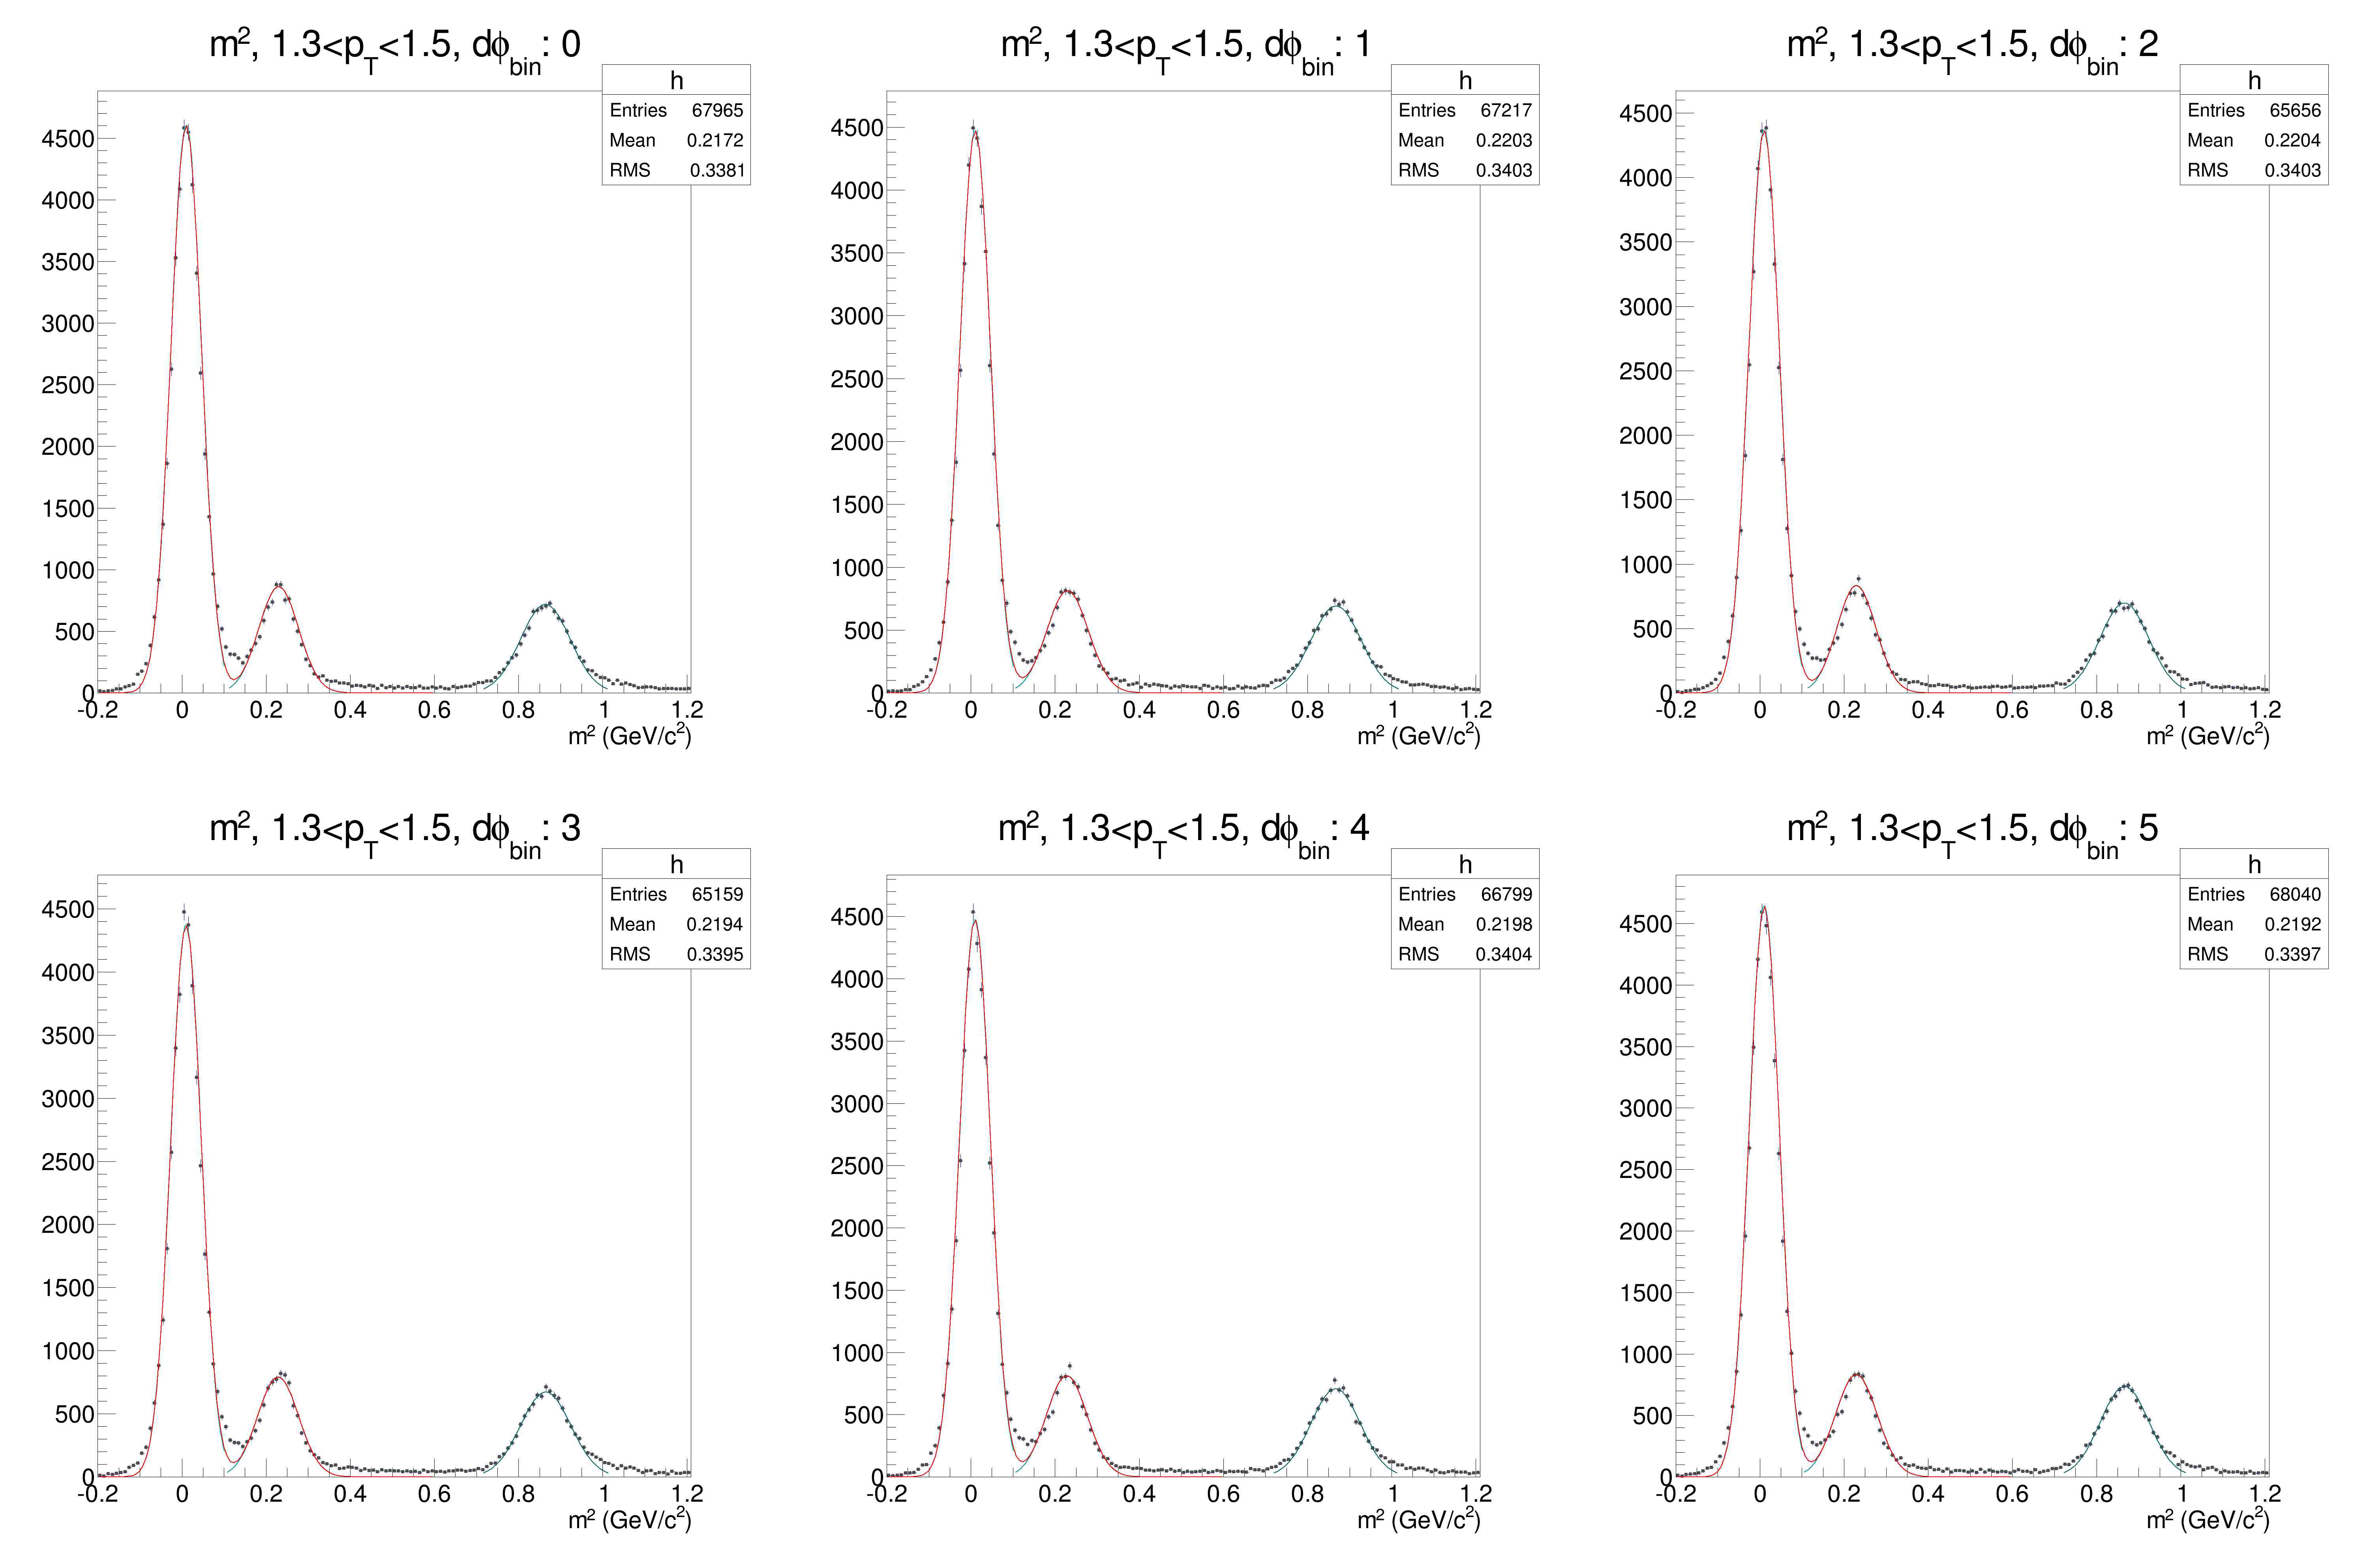
\includegraphics[width=1\textwidth]{lowptfits/yieldvsdphi_tof1_cent0_ch0_pT-13-15.jpg}
    \end{subfigure}
    \begin{subfigure}{1\textwidth}
    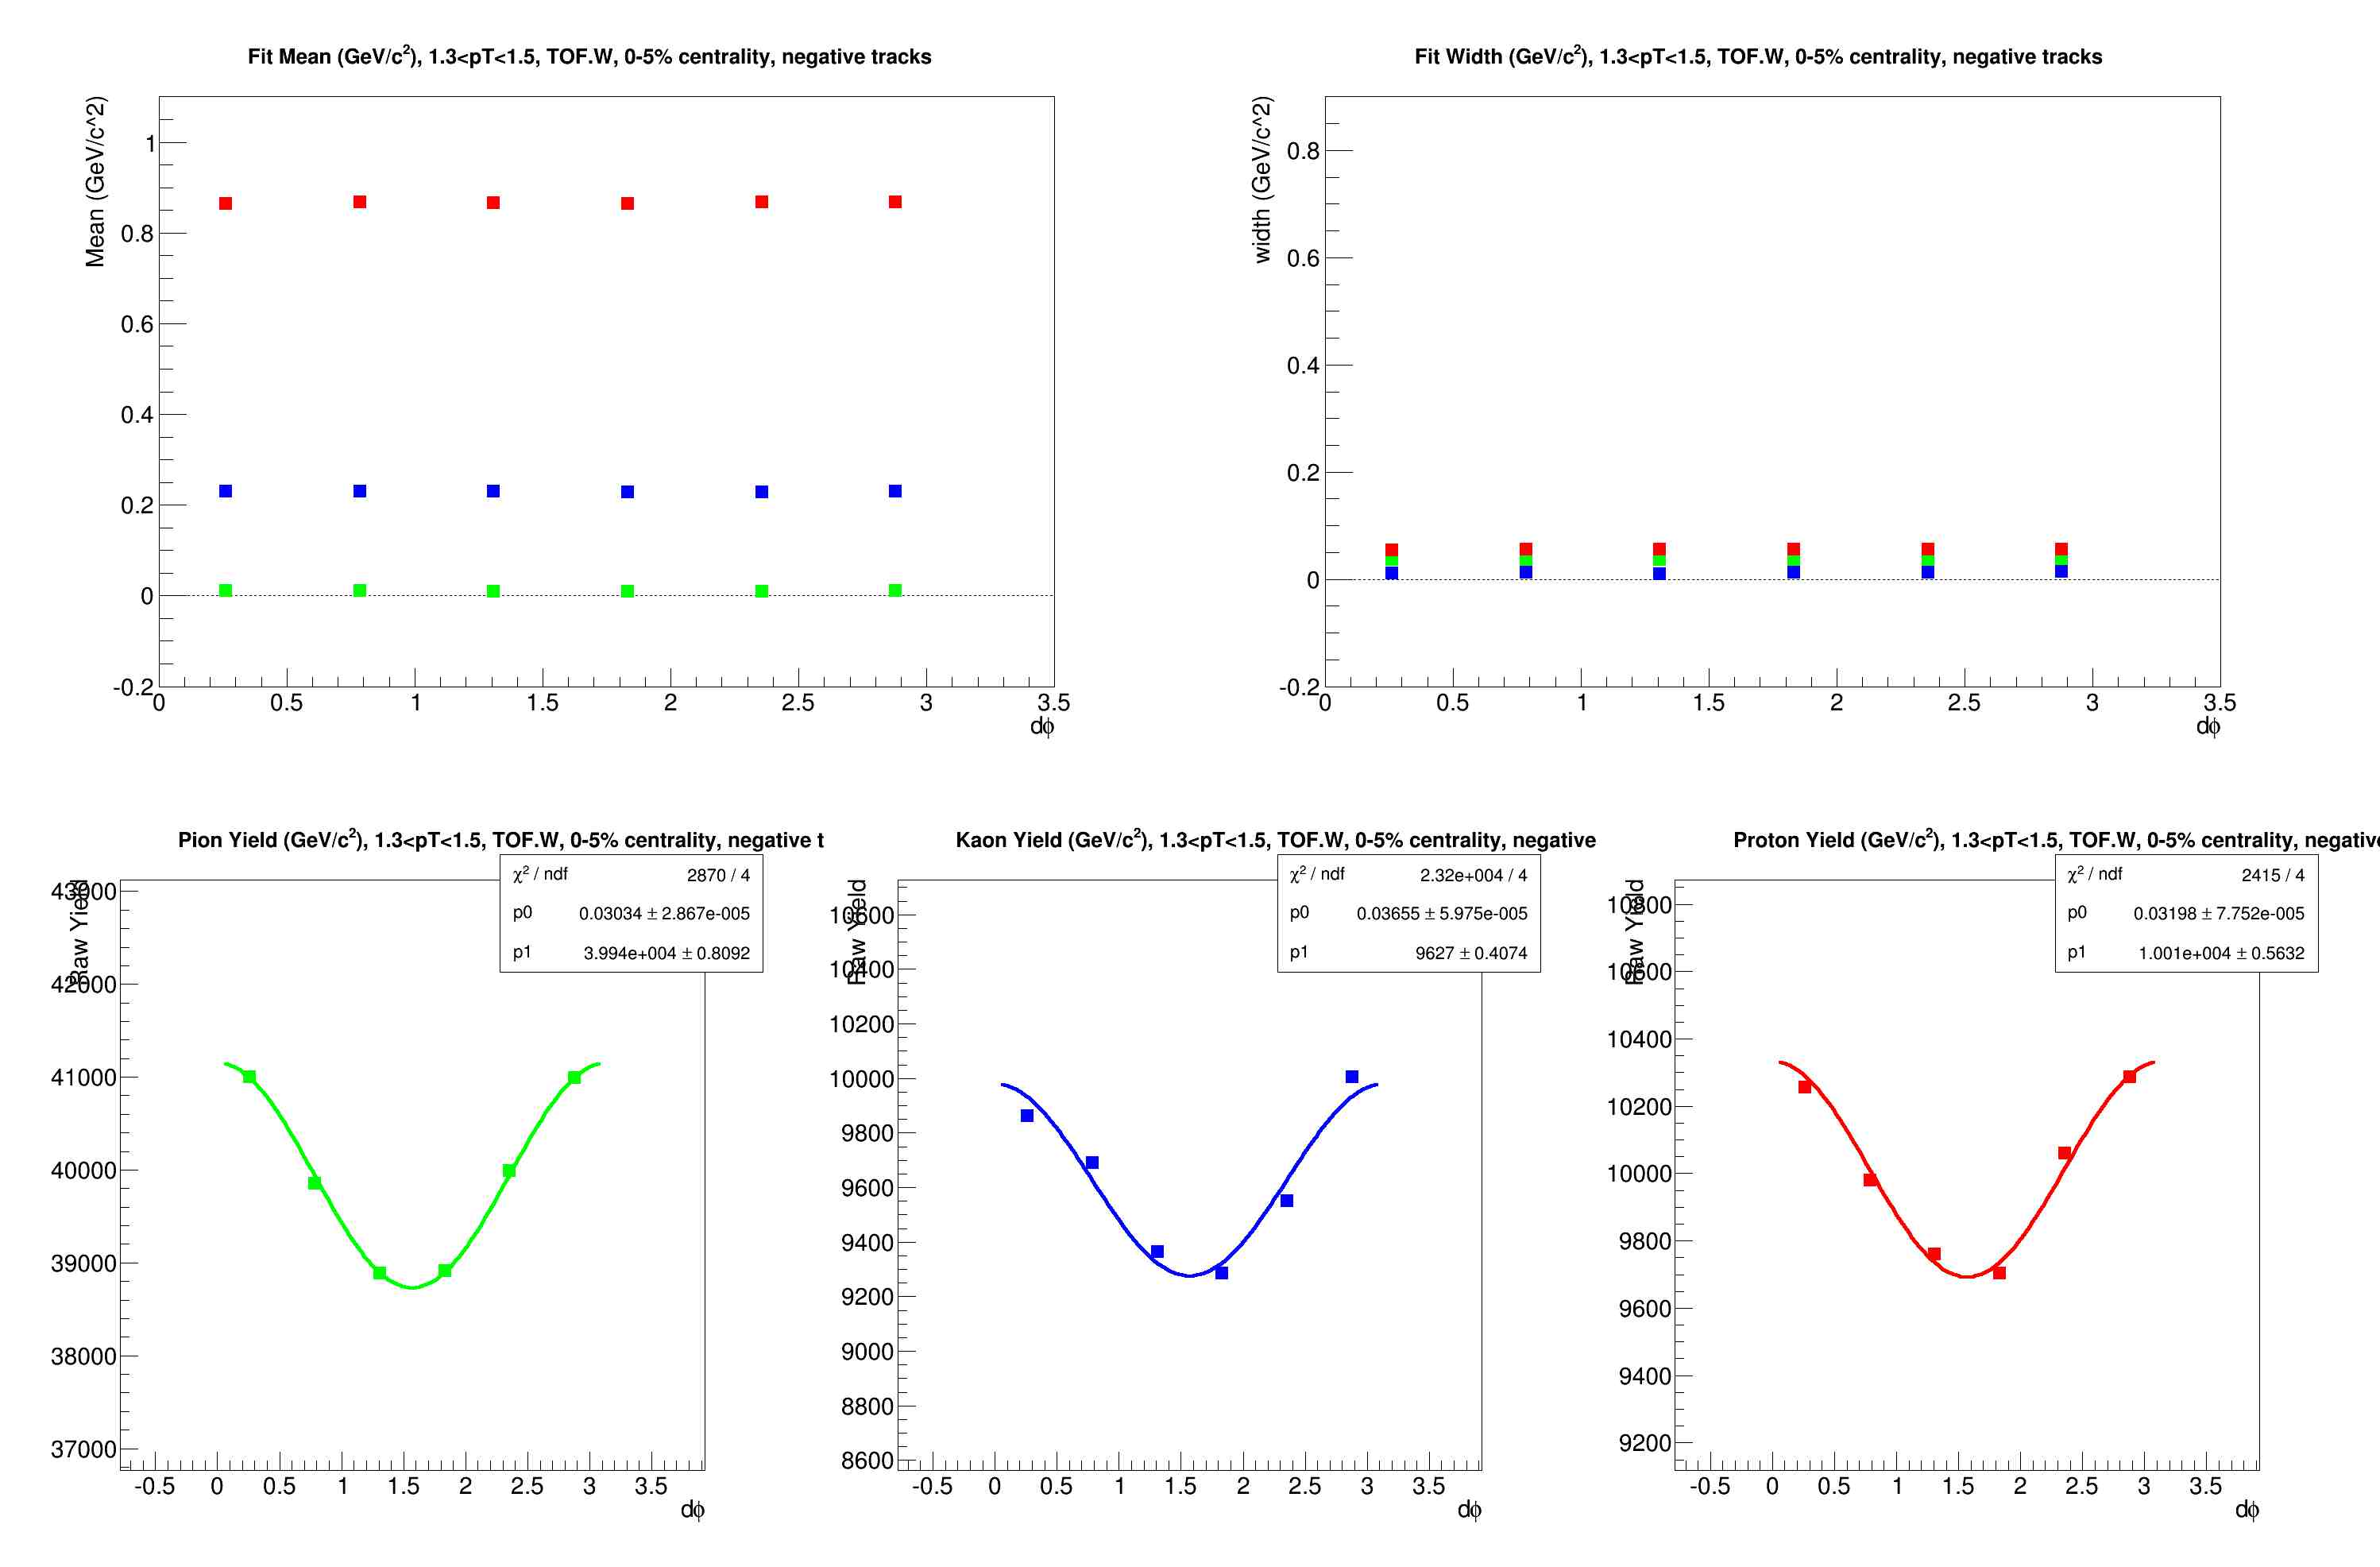
\includegraphics[width=1\textwidth]{lowptfits/fitParams_tof1_cent0_ch0_pT-13-15.jpg}
    \end{subfigure}
    \rule{35em}{0.5pt}
  \caption[PID fits and Yield vs $d\phi$ for $p_T$=1.3-1.5 GeV/c, TOF.W, negative particles ]{$m^2$ Gaussian fits for PID and resulting Yield vs $d\phi$ for $p_T$=1.3-1.5 GeV/c, TOF.W, negative particles}
  \label{fig:fits13-15neg}
\end{figure}

\begin{figure}[H]
  \centering
    \begin{subfigure}{1\textwidth}
    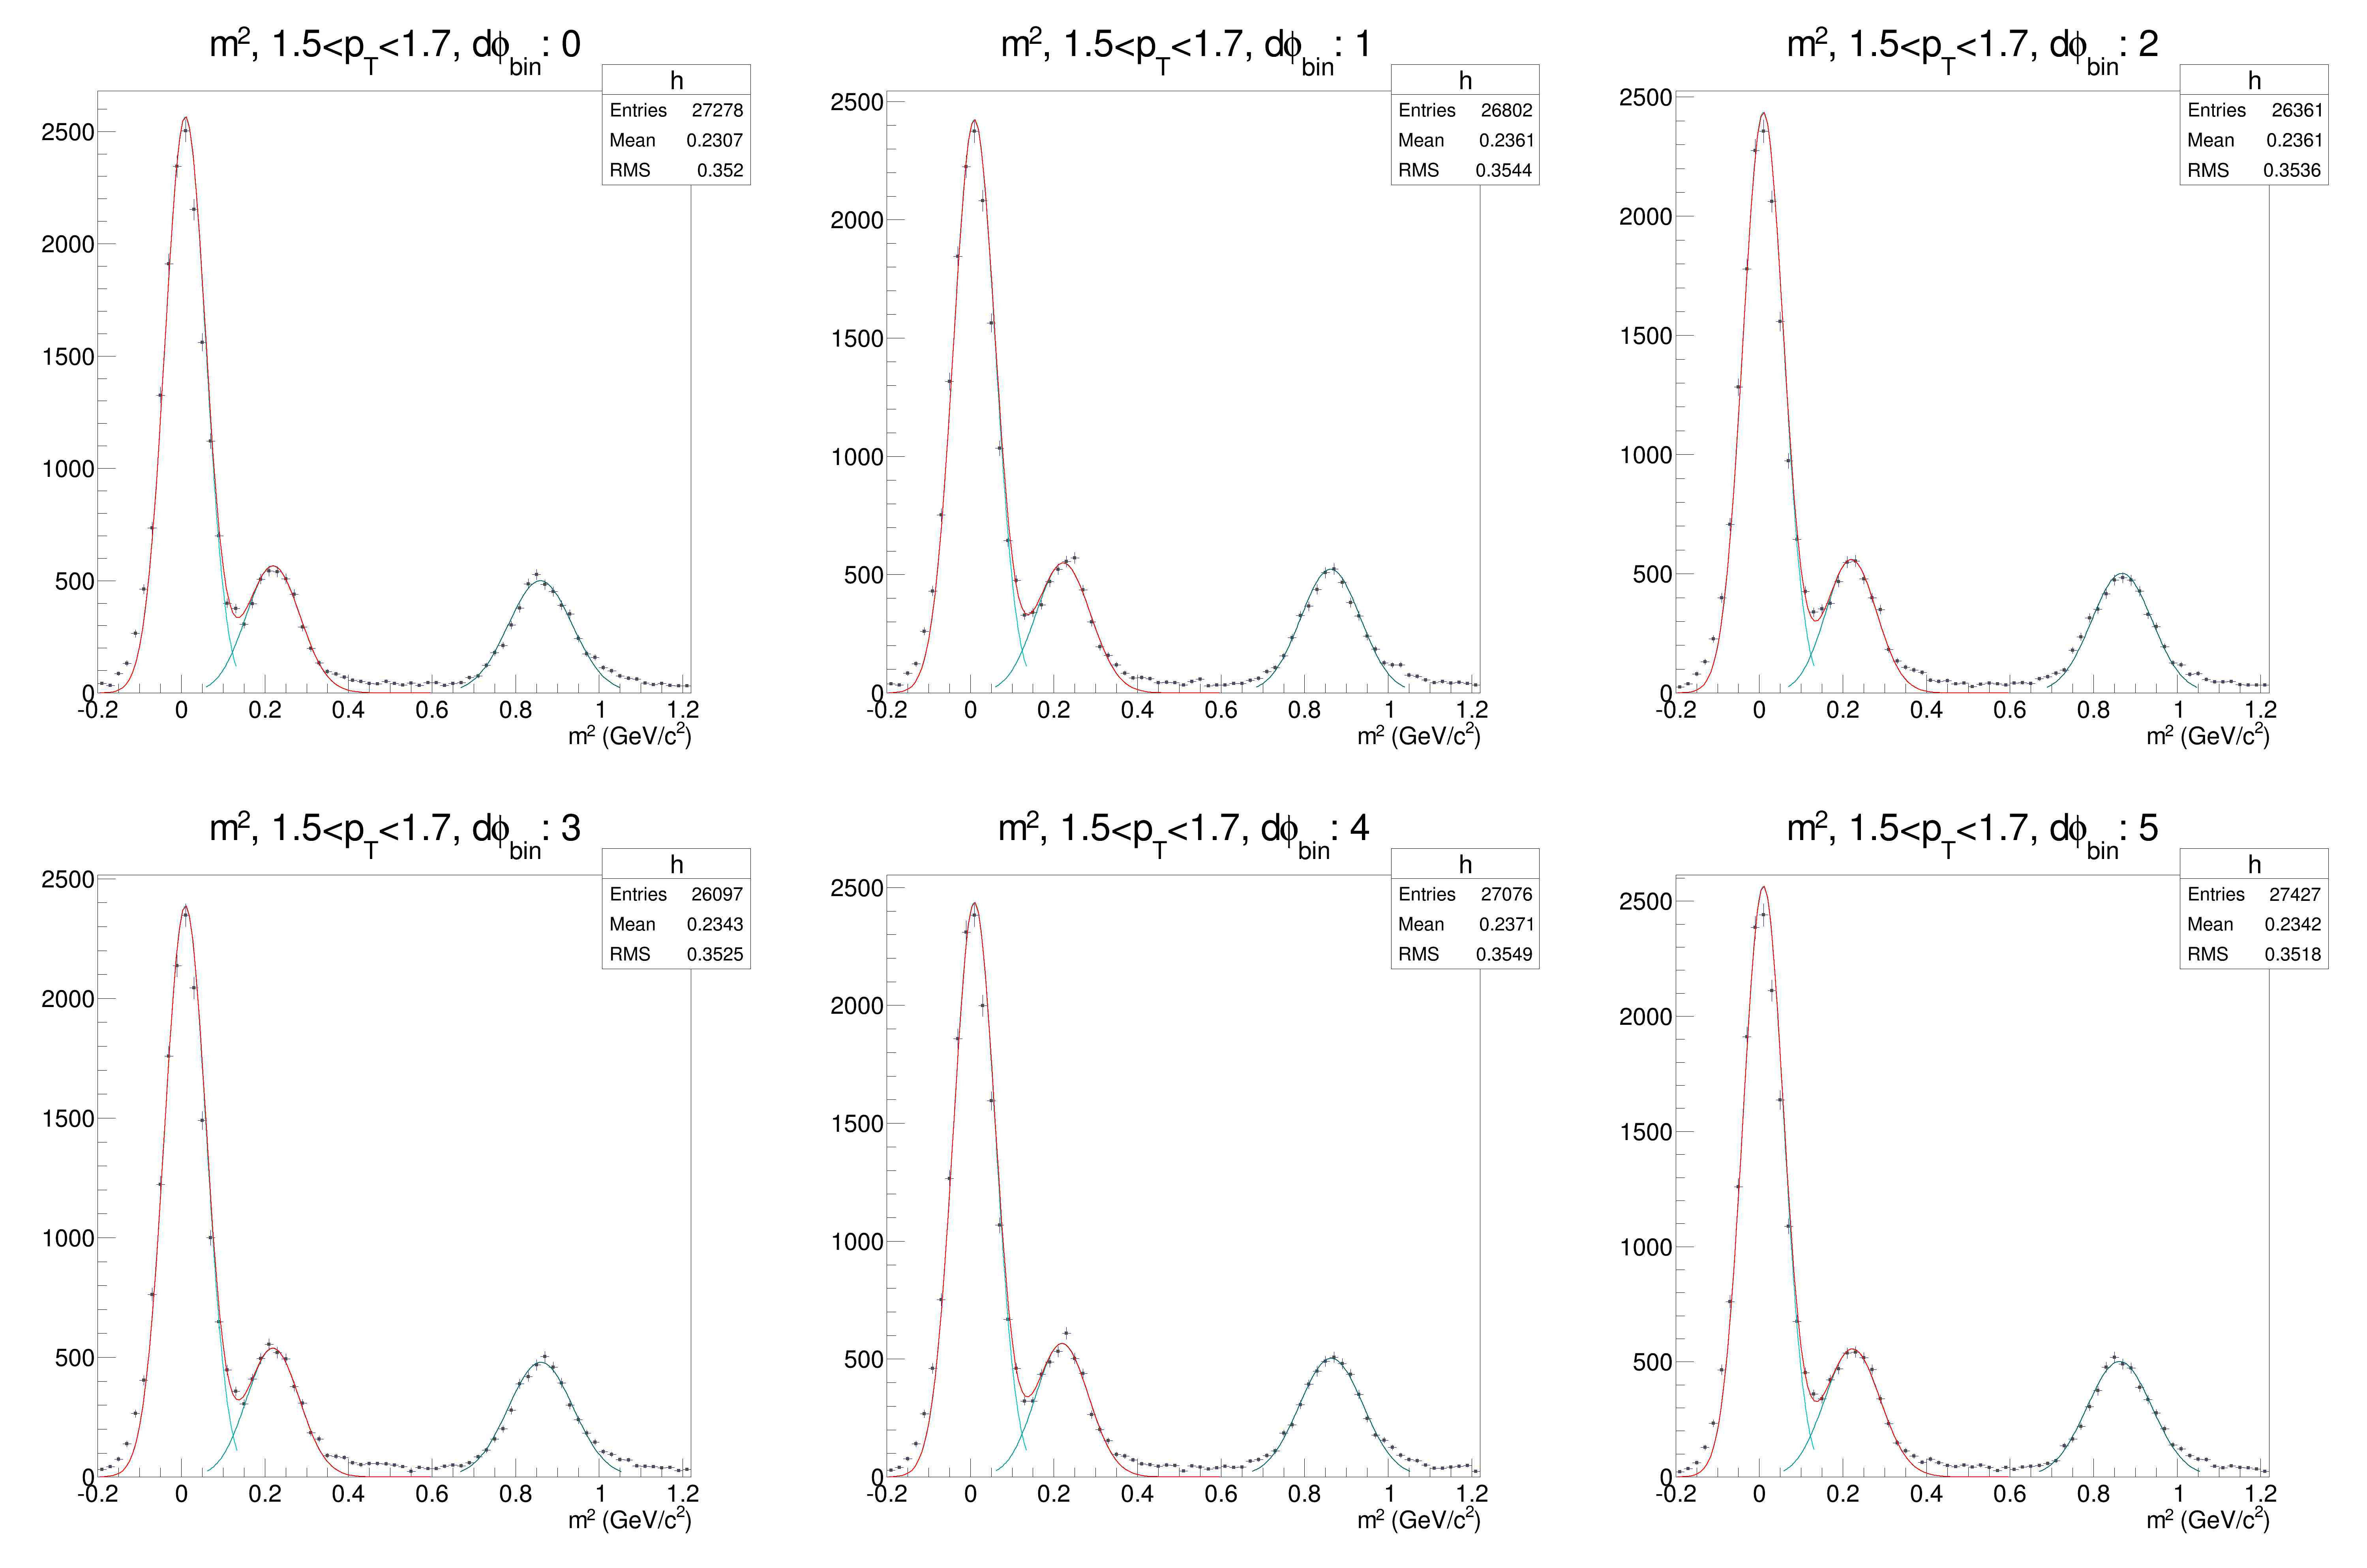
\includegraphics[width=1\textwidth]{lowptfits/yieldvsdphi_tof1_cent0_ch0_pT-15-17.jpg}
    \end{subfigure}
    \begin{subfigure}{1\textwidth}
    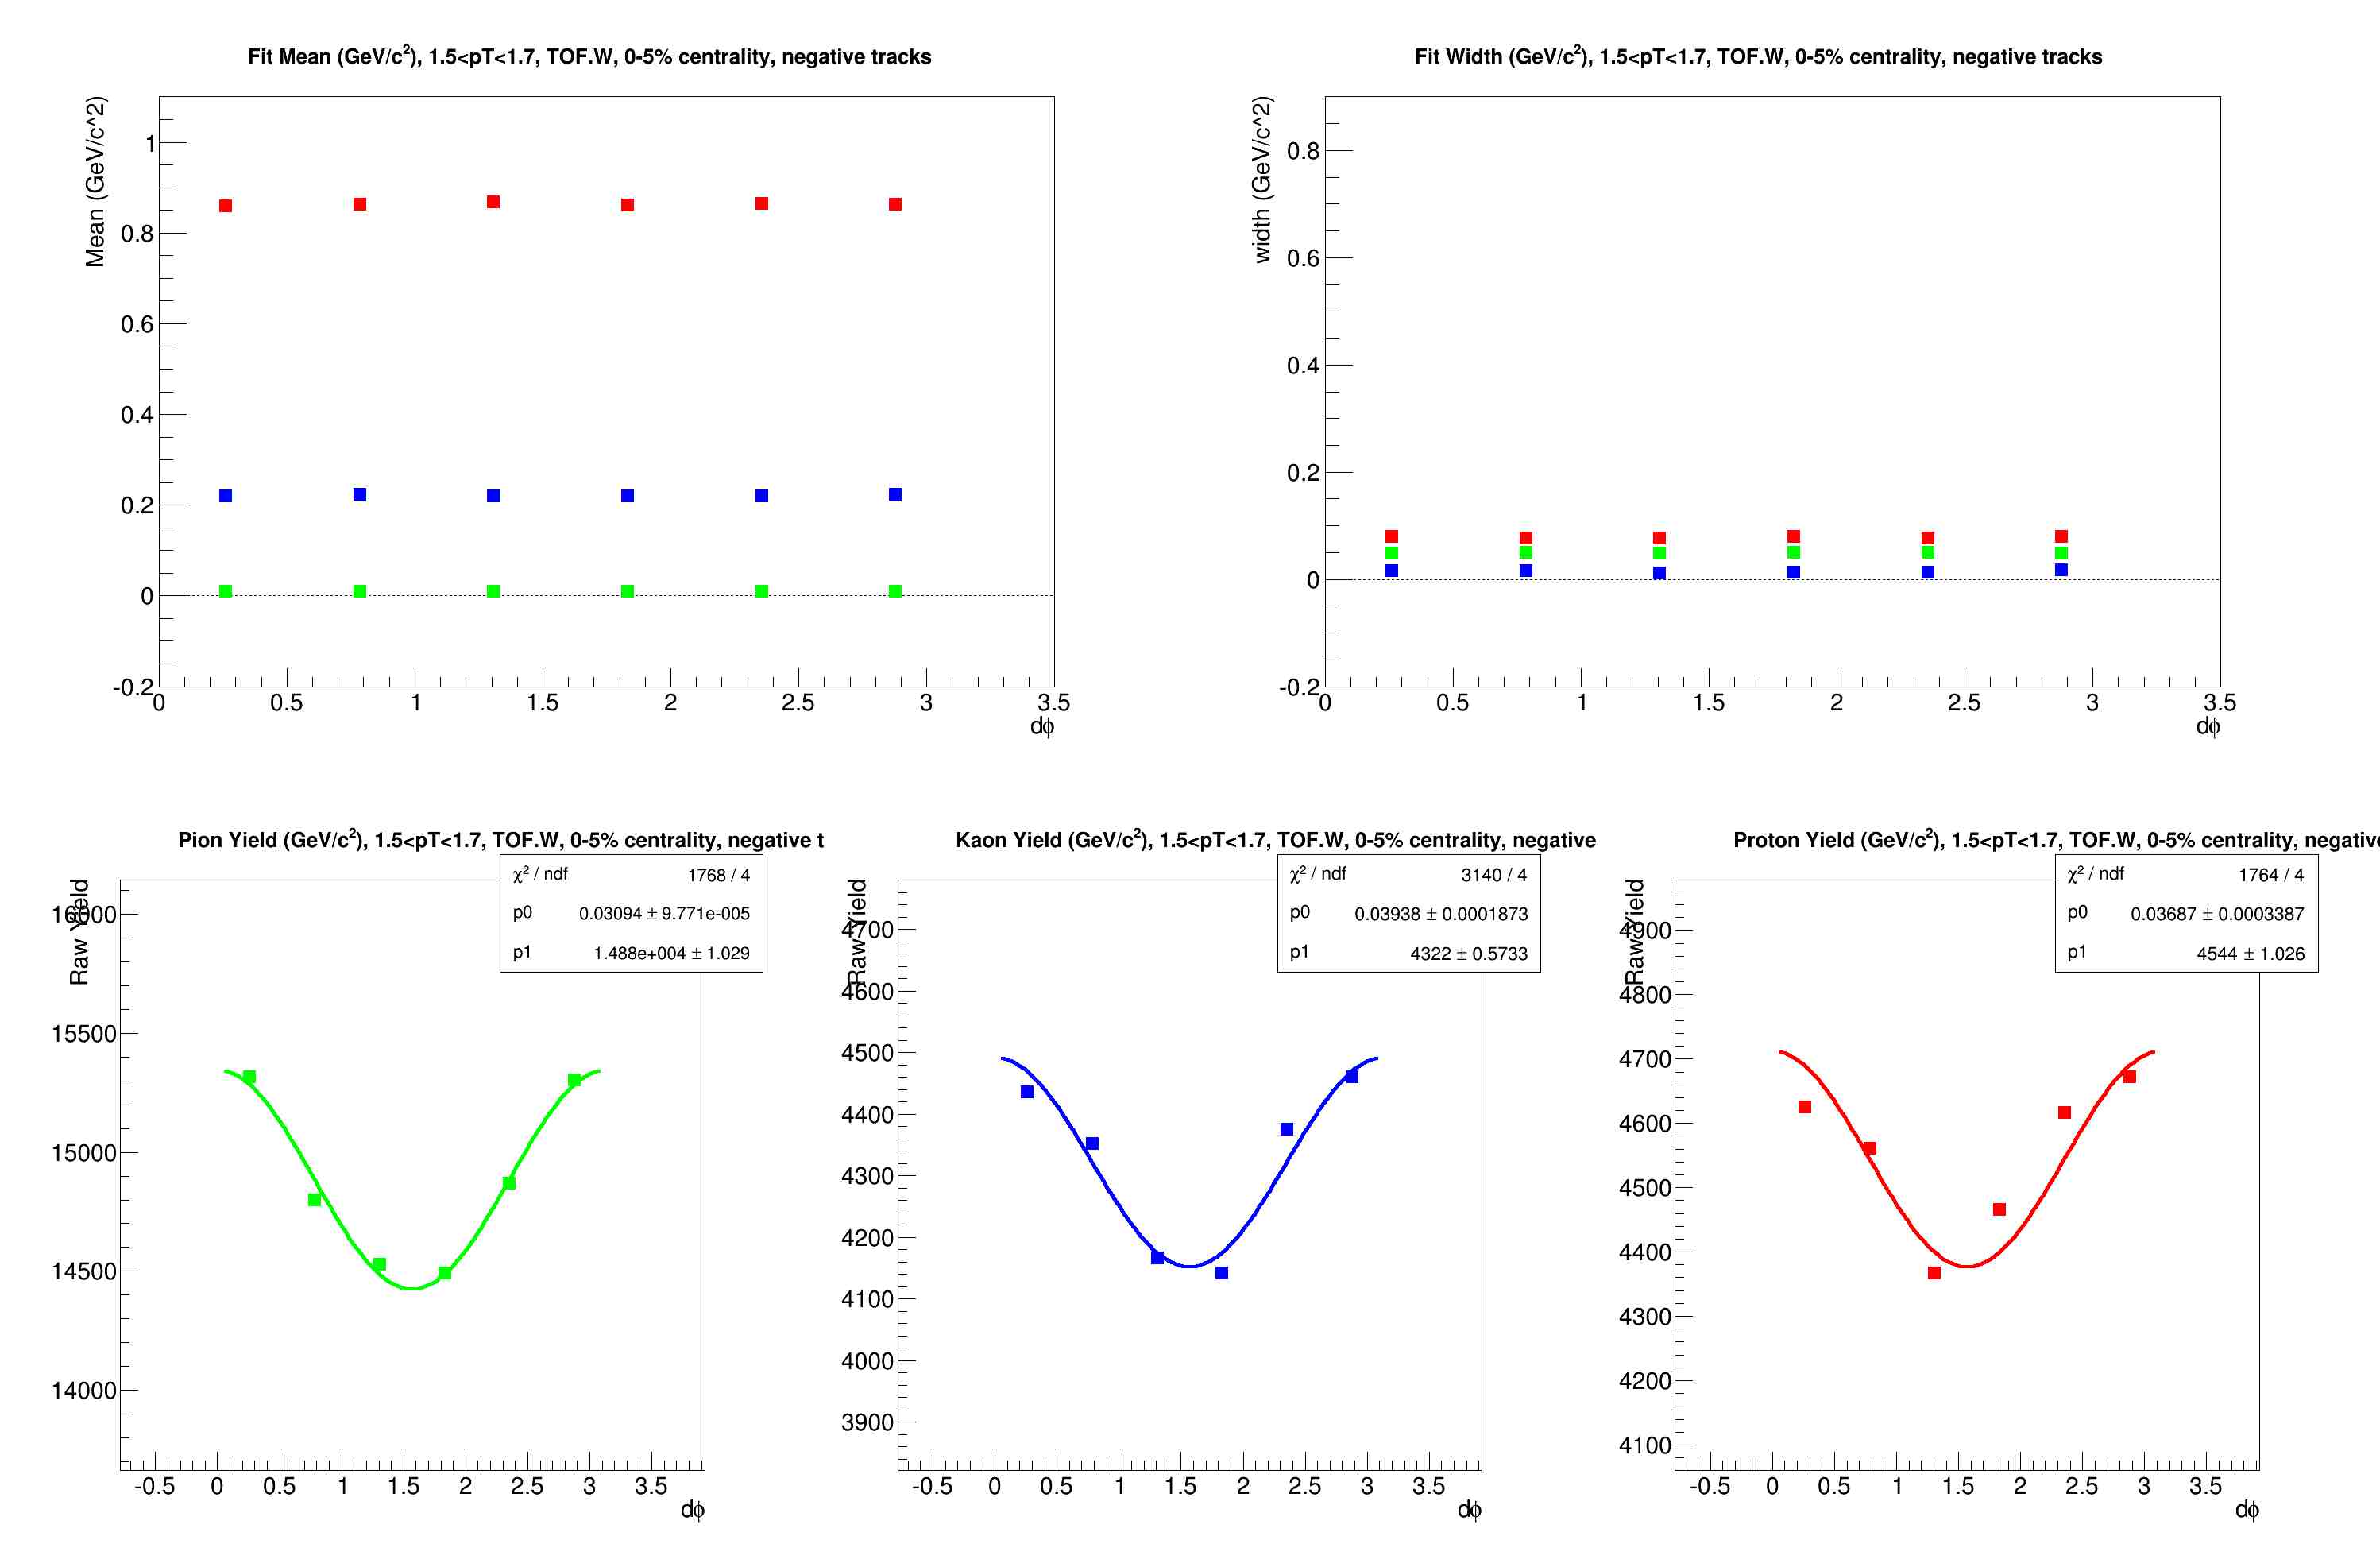
\includegraphics[width=1\textwidth]{lowptfits/fitParams_tof1_cent0_ch0_pT-15-17.jpg}
    \end{subfigure}
    \rule{35em}{0.5pt}
  \caption[PID fits and Yield vs $d\phi$ for $p_T$=1.5-1.7 GeV/c, TOF.W, negative particles ]{$m^2$ Gaussian fits for PID and resulting Yield vs $d\phi$ for $p_T$=1.5-1.7 GeV/c, TOF.W, negative particles}
  \label{fig:fits15-17neg}
\end{figure}

\begin{figure}[H]
  \centering
    \begin{subfigure}[p]{1\textwidth}
    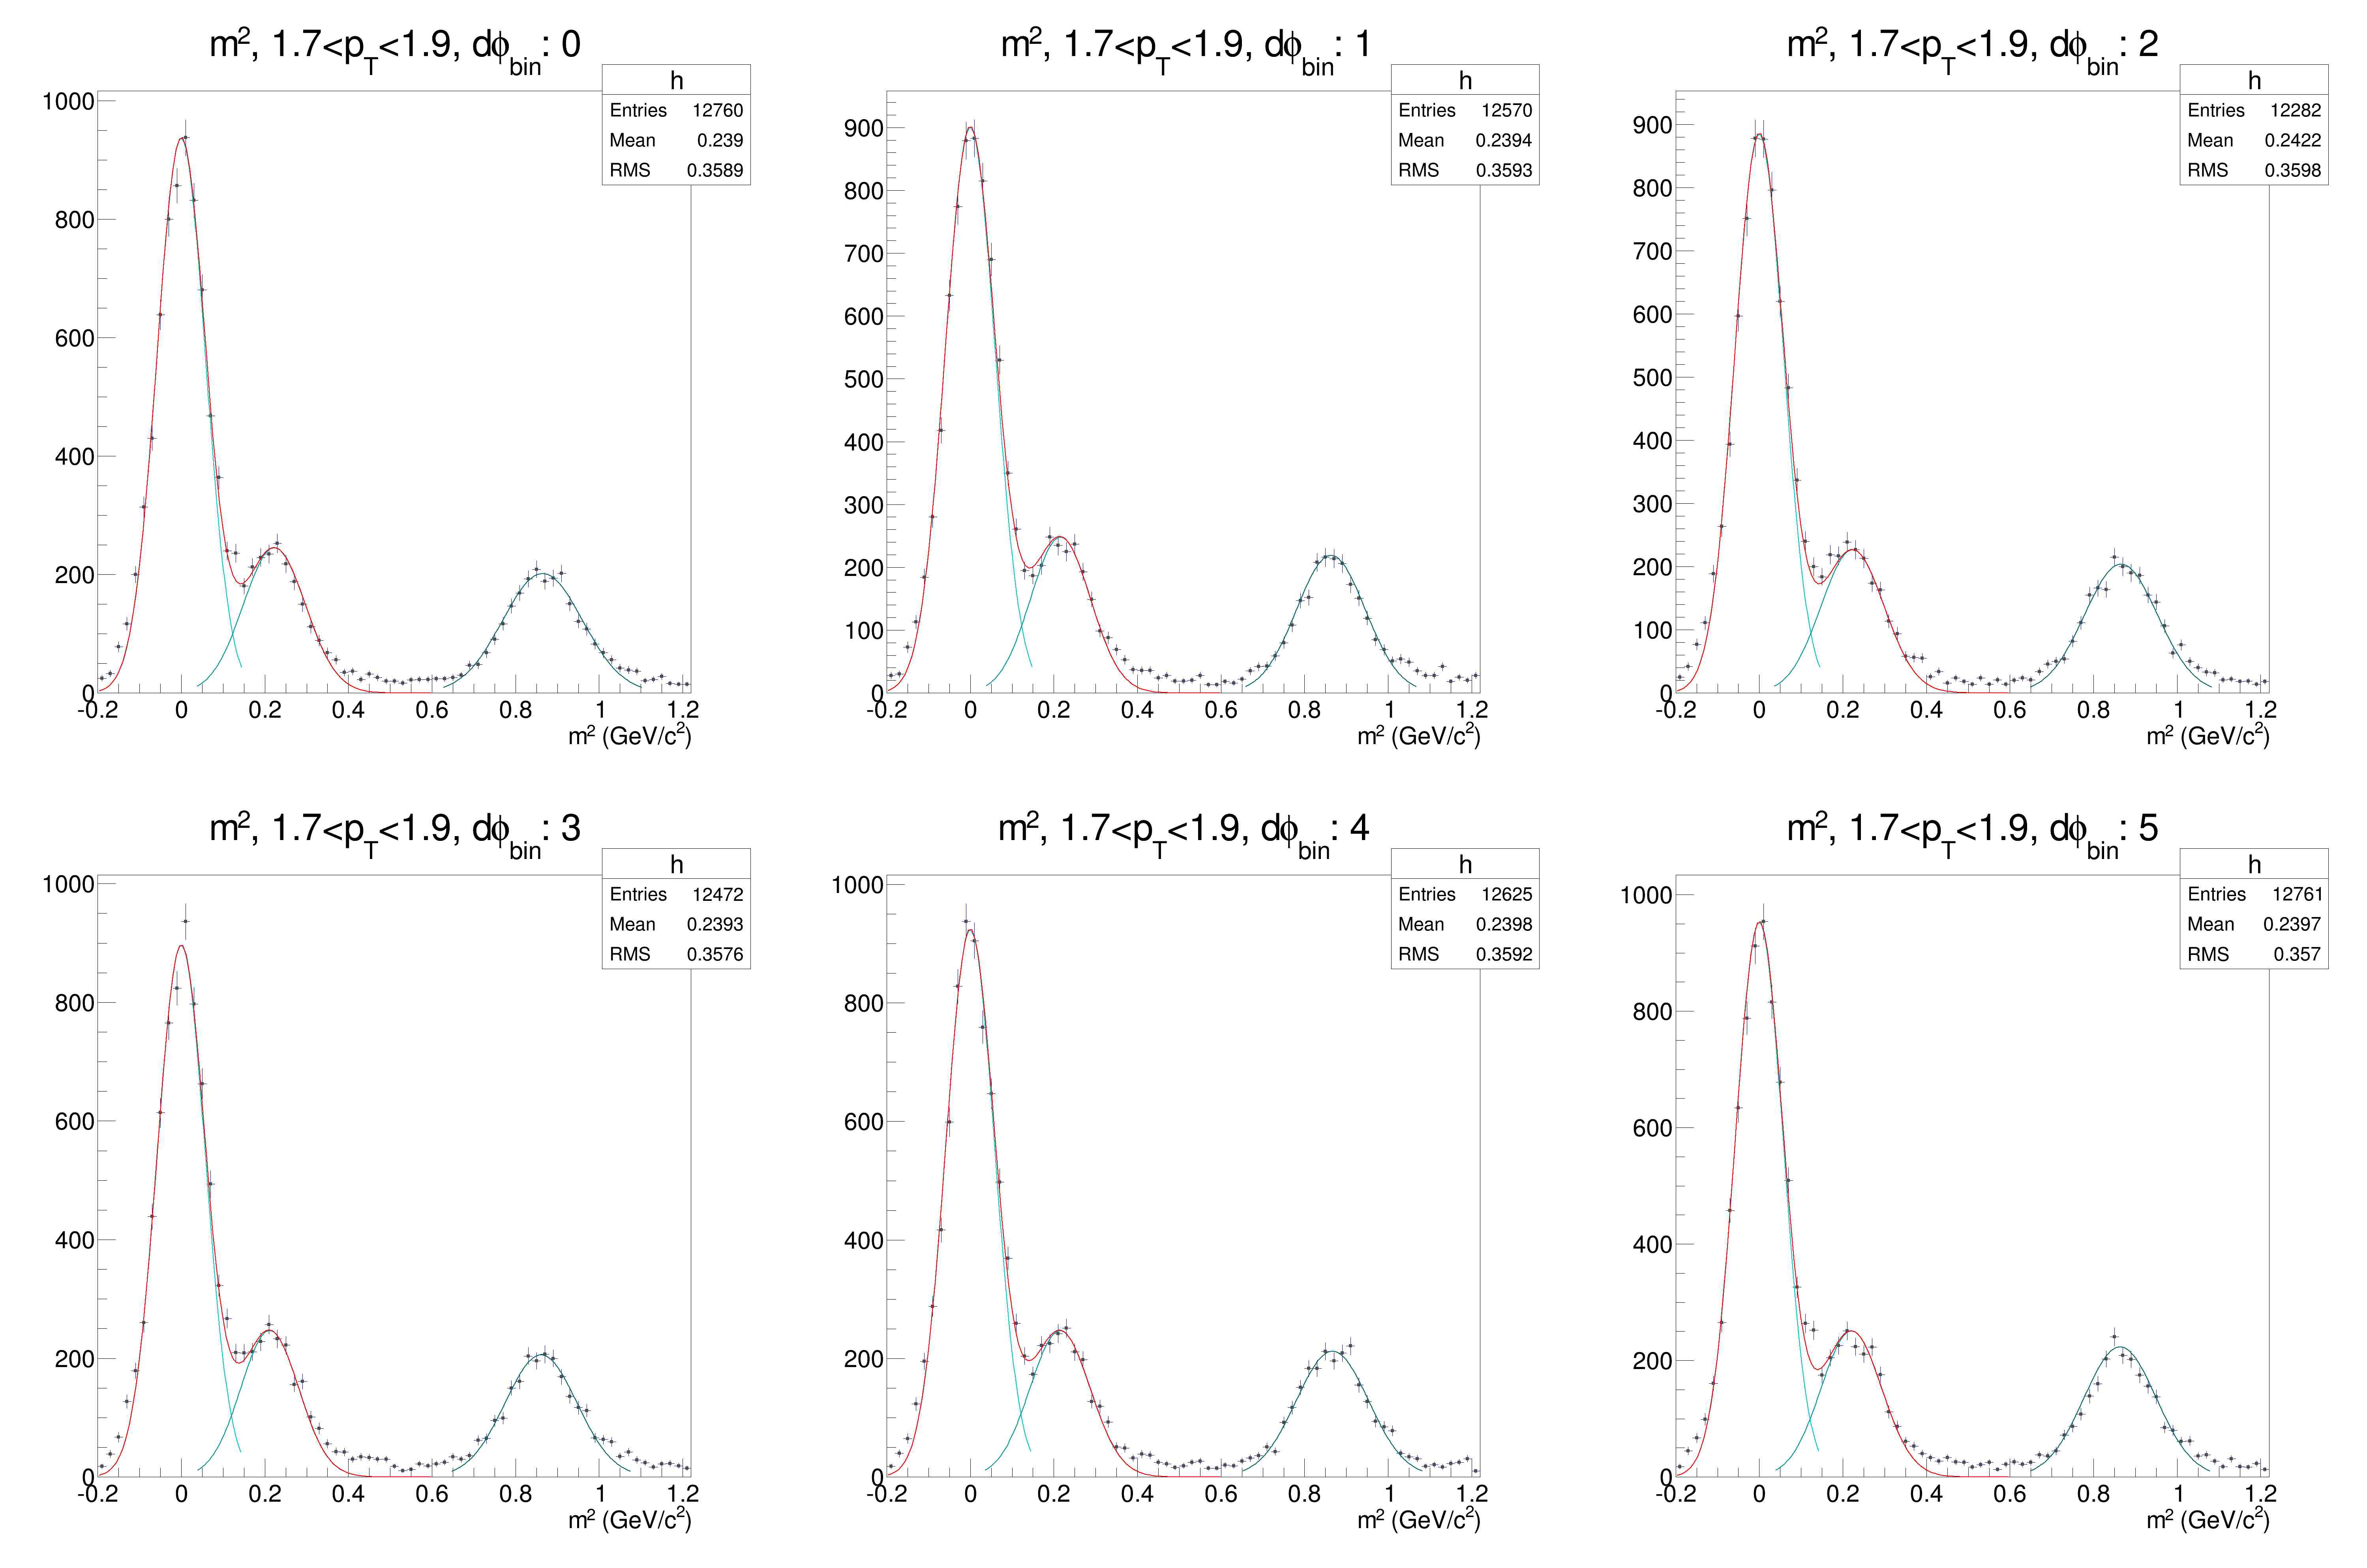
\includegraphics[width=1\textwidth]{lowptfits/yieldvsdphi_tof1_cent0_ch0_pT-17-19.jpg}
    \end{subfigure}
    \begin{subfigure}[p]{1\textwidth}
    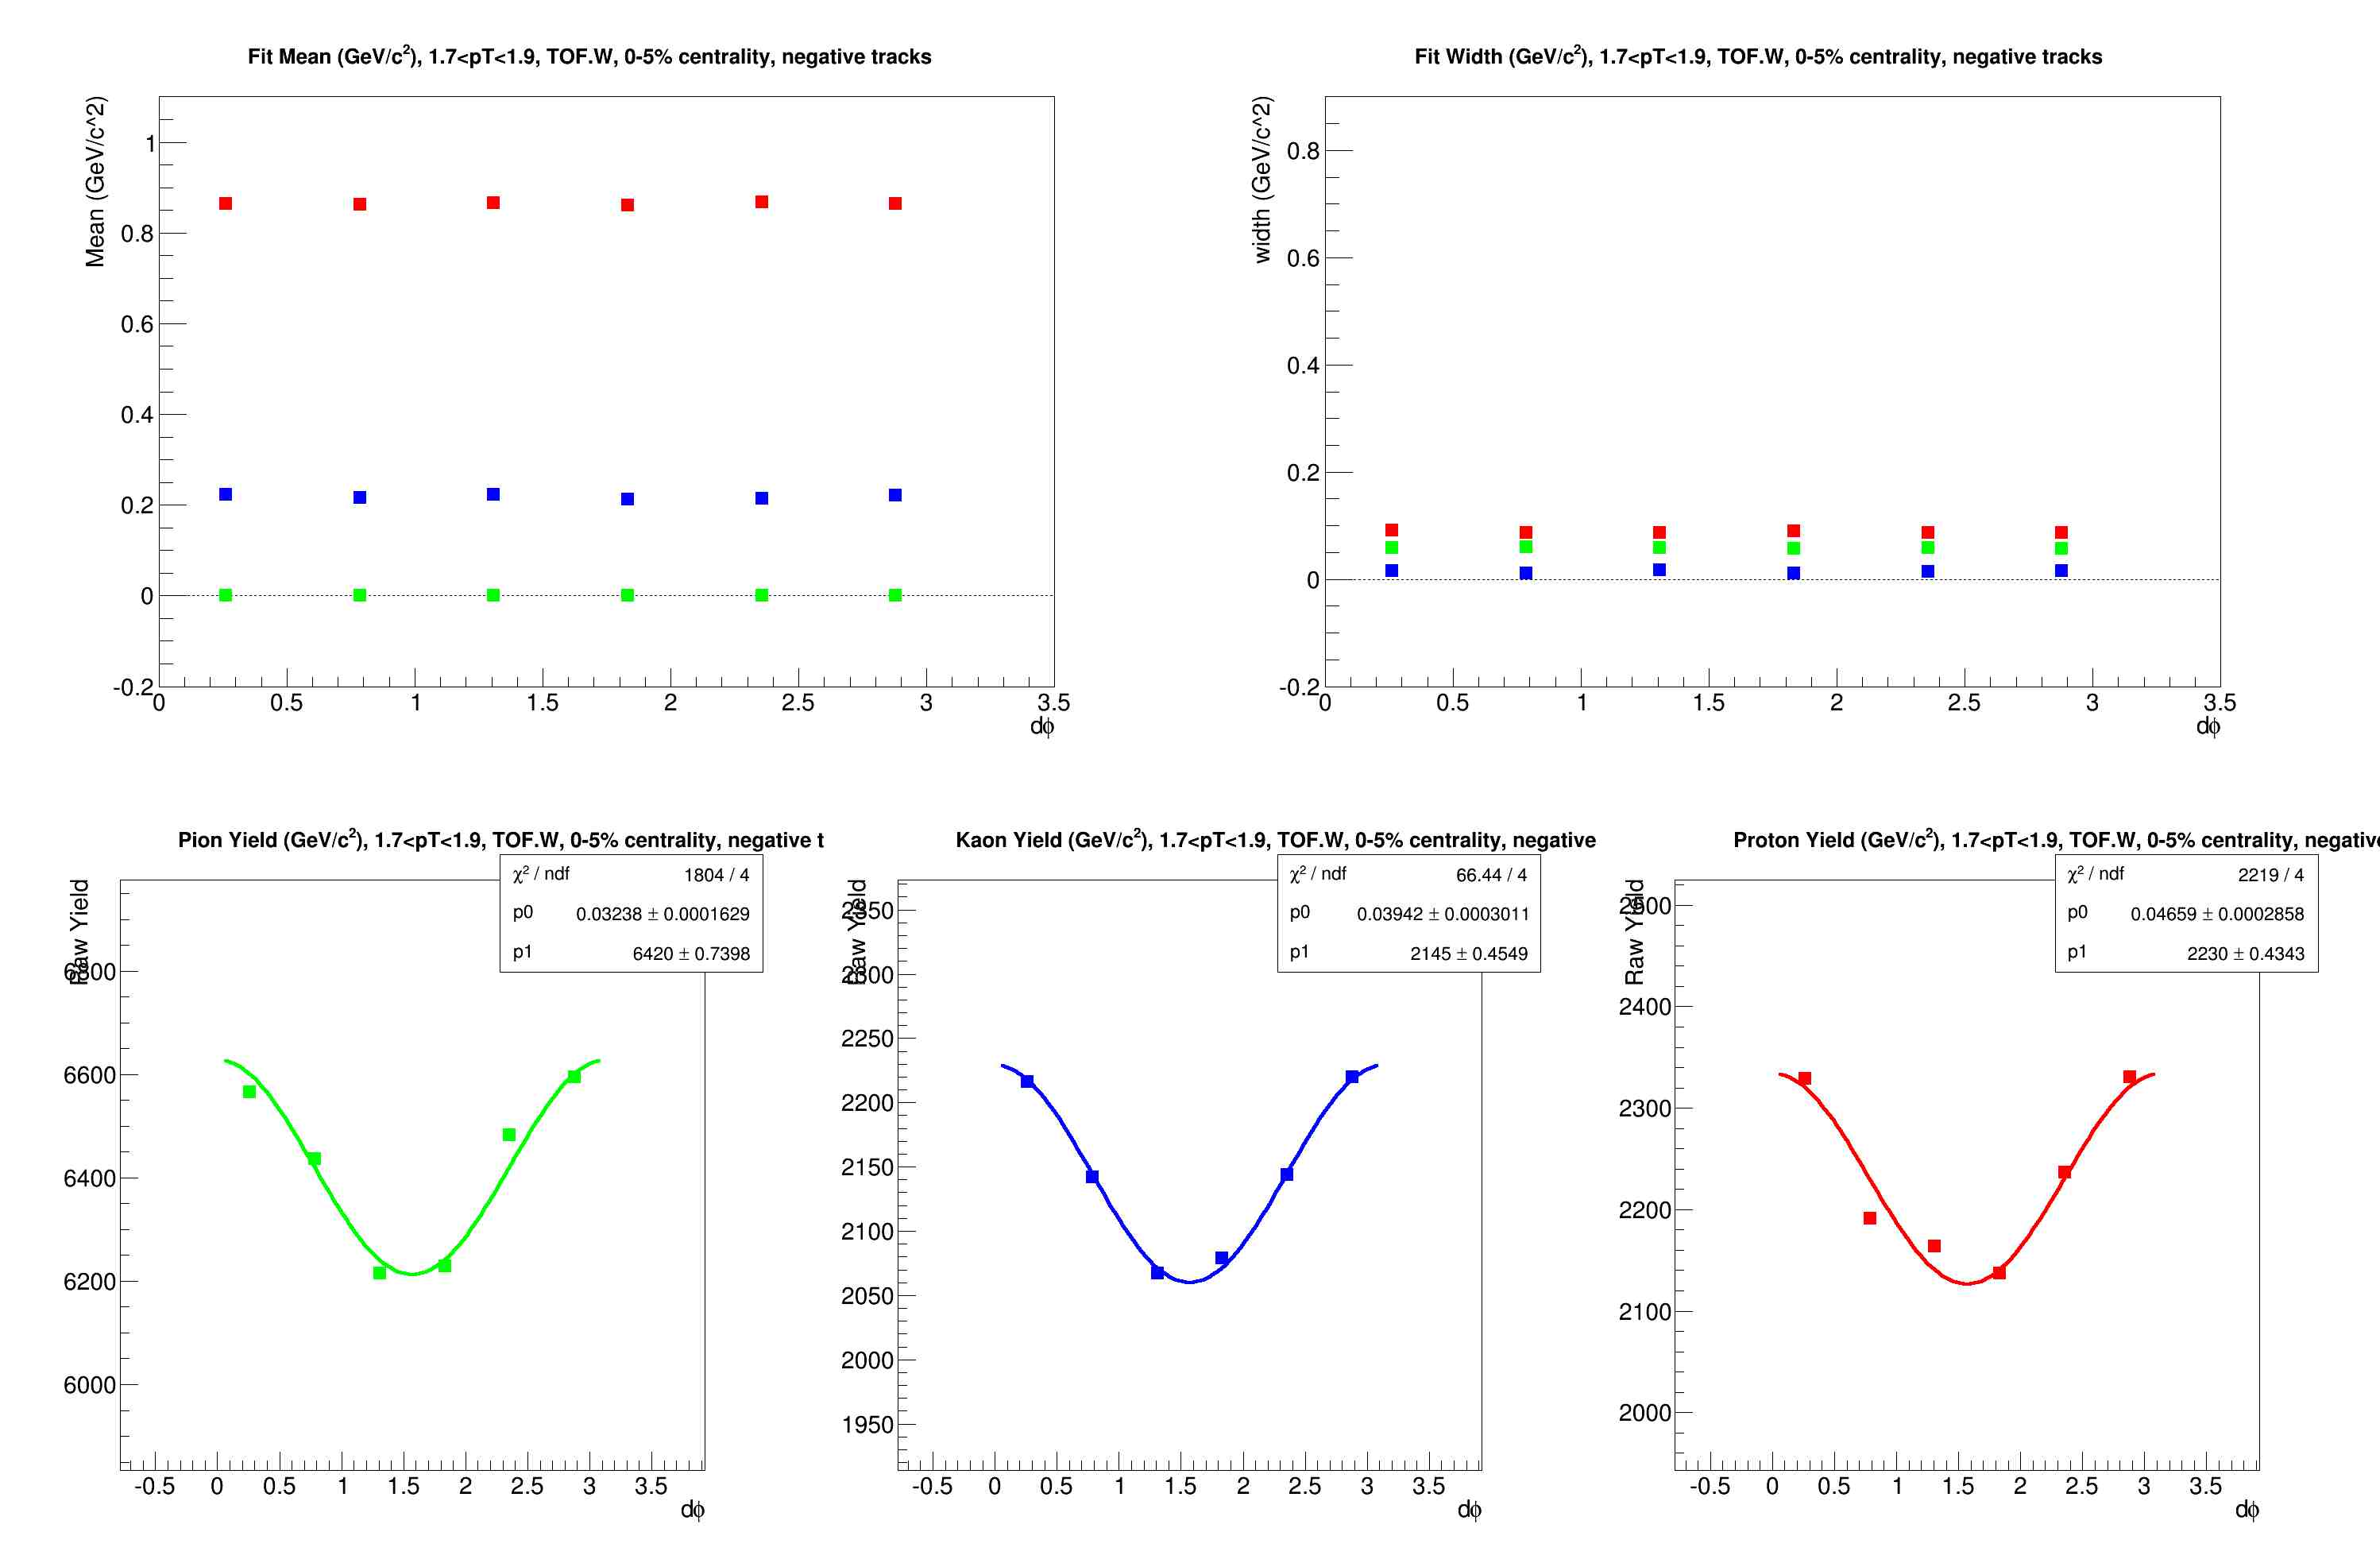
\includegraphics[width=1\textwidth]{lowptfits/fitParams_tof1_cent0_ch0_pT-17-19.jpg}
    \end{subfigure}
    \rule{35em}{0.5pt}
  \caption[PID fits and Yield vs $d\phi$ for $p_T$=1.7-1.9 GeV/c, TOF.W, negative particles ]{$m^2$ Gaussian fits for PID and resulting Yield vs $d\phi$ for $p_T$=1.7-1.9 GeV/c, TOF.W, negative particles}
  \label{fig:fits17-19neg}
\end{figure}

\begin{figure}[H]
  \centering
    \begin{subfigure}[p]{1\textwidth}
    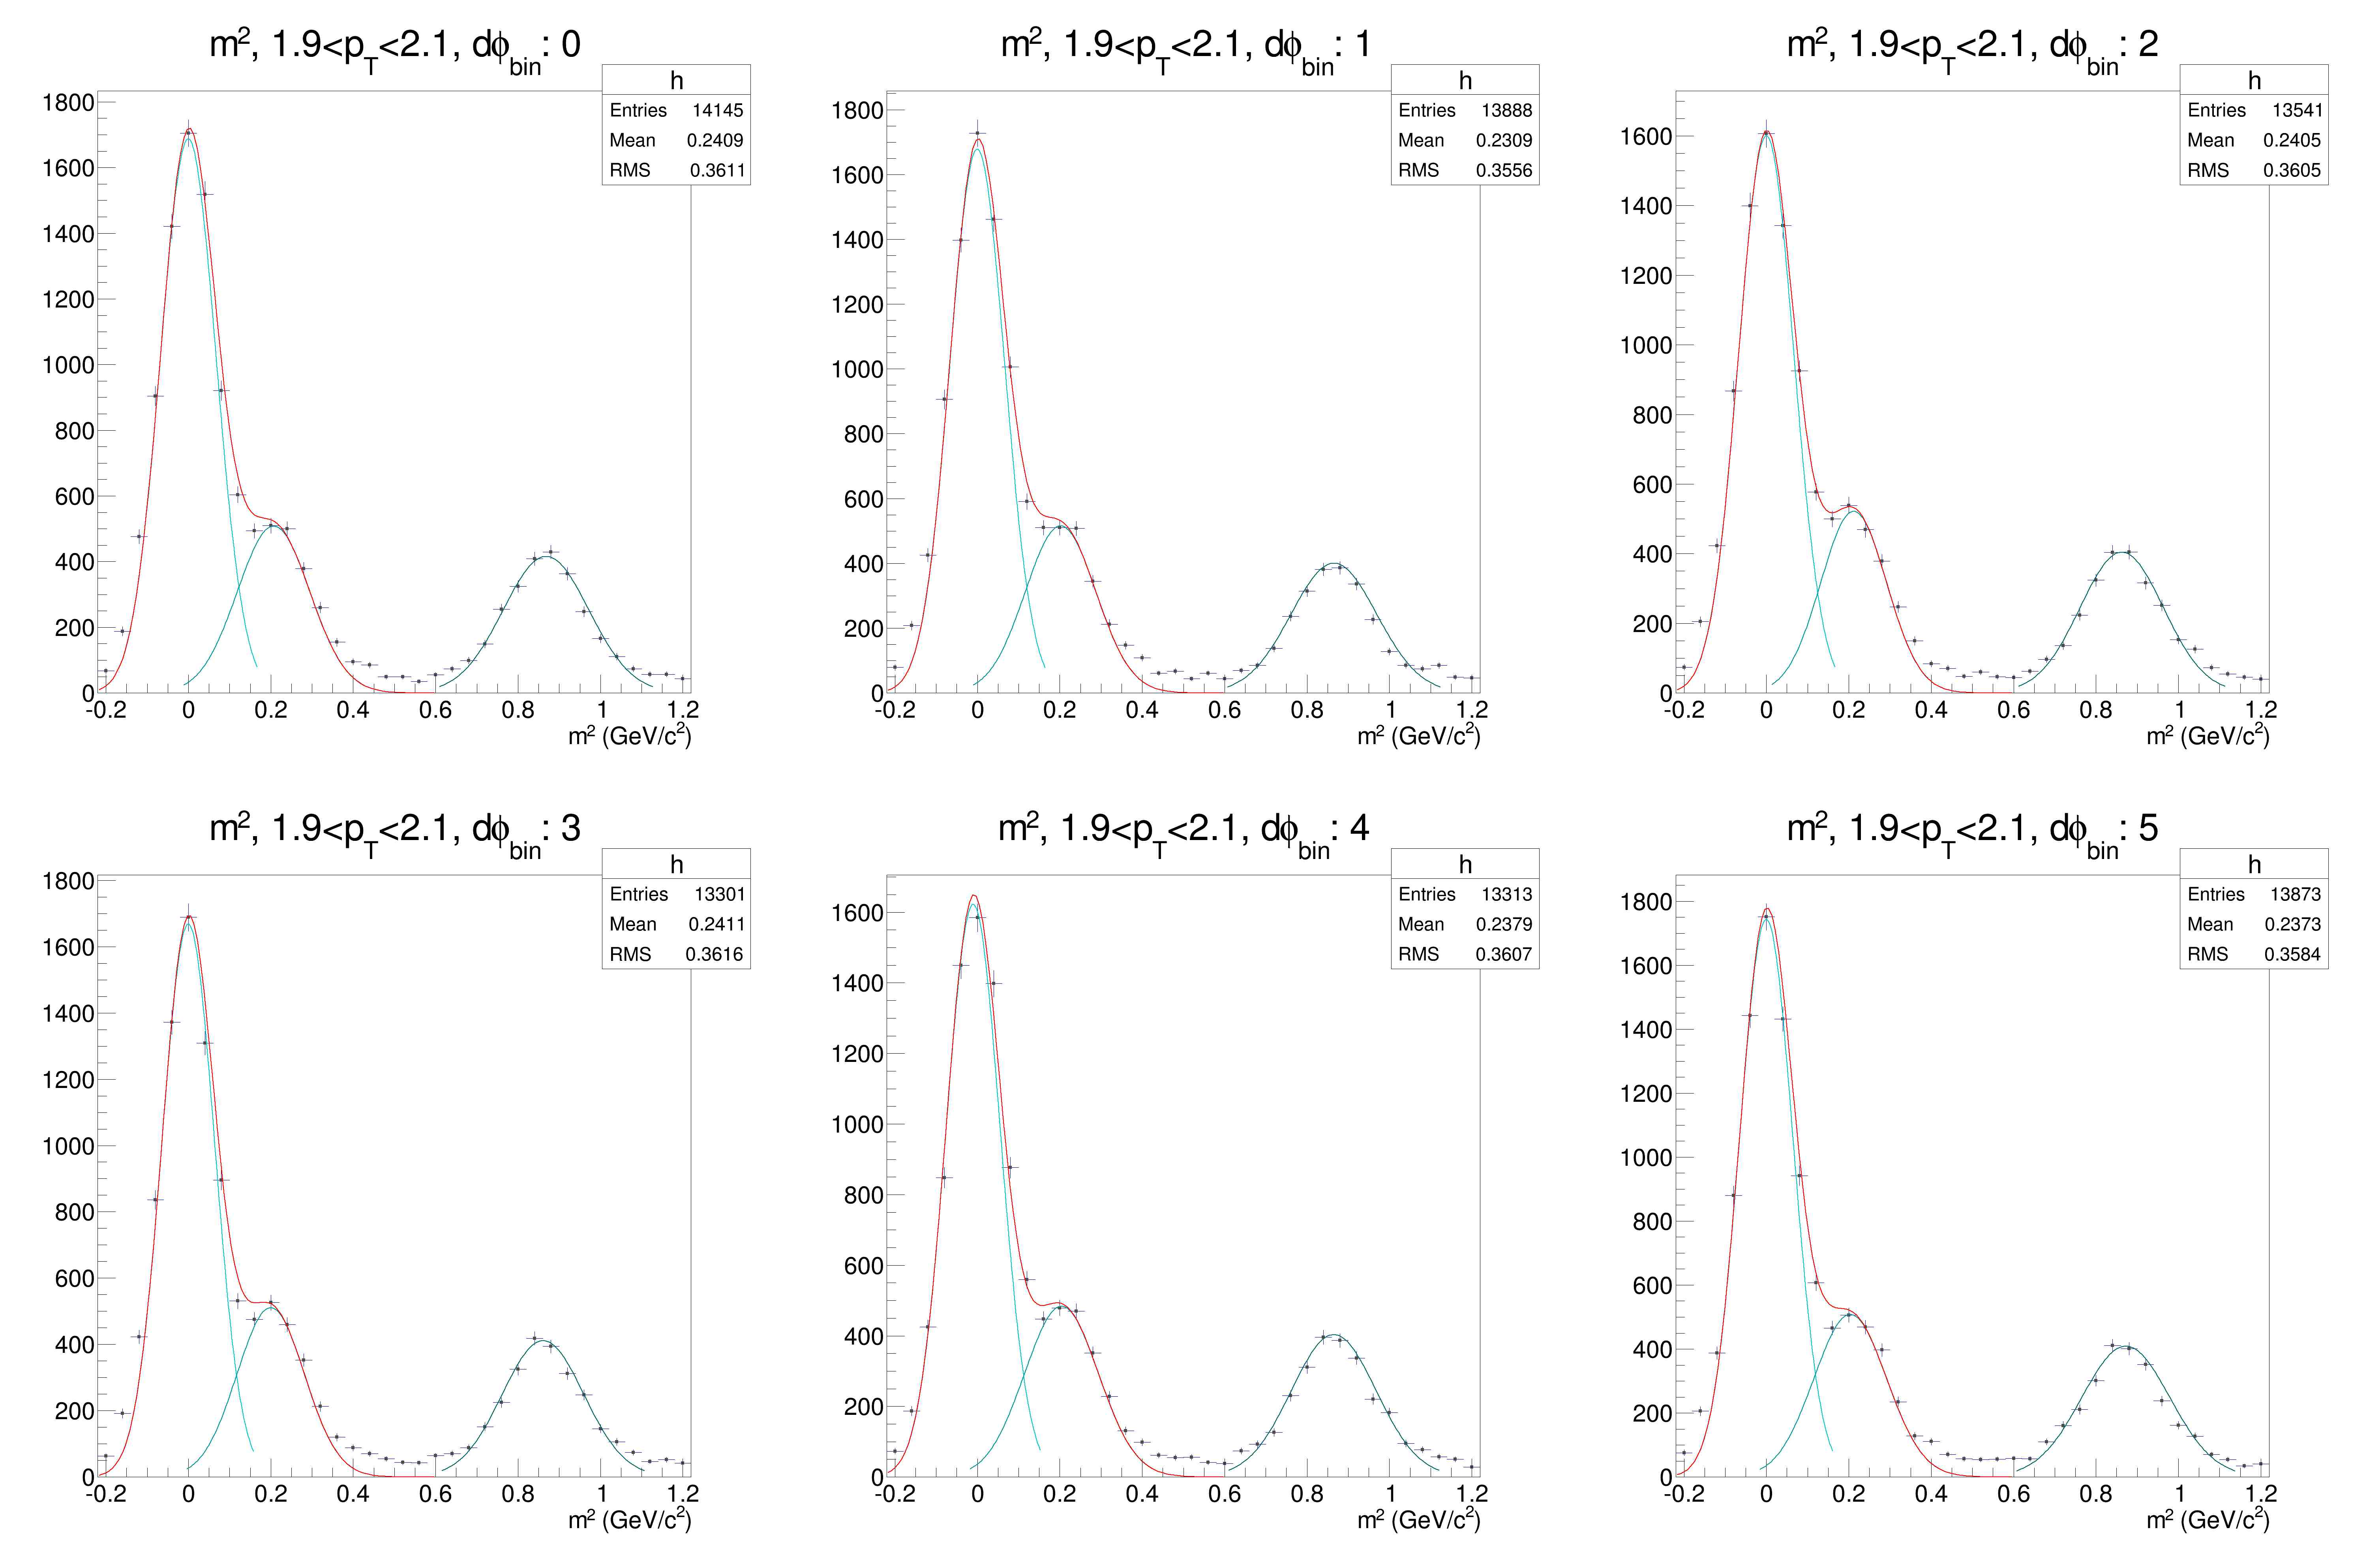
\includegraphics[width=1\textwidth]{lowptfits/yieldvsdphi_tof1_cent0_ch0_pT-19-21.jpg}
    \end{subfigure}
    \begin{subfigure}[p]{1\textwidth}
    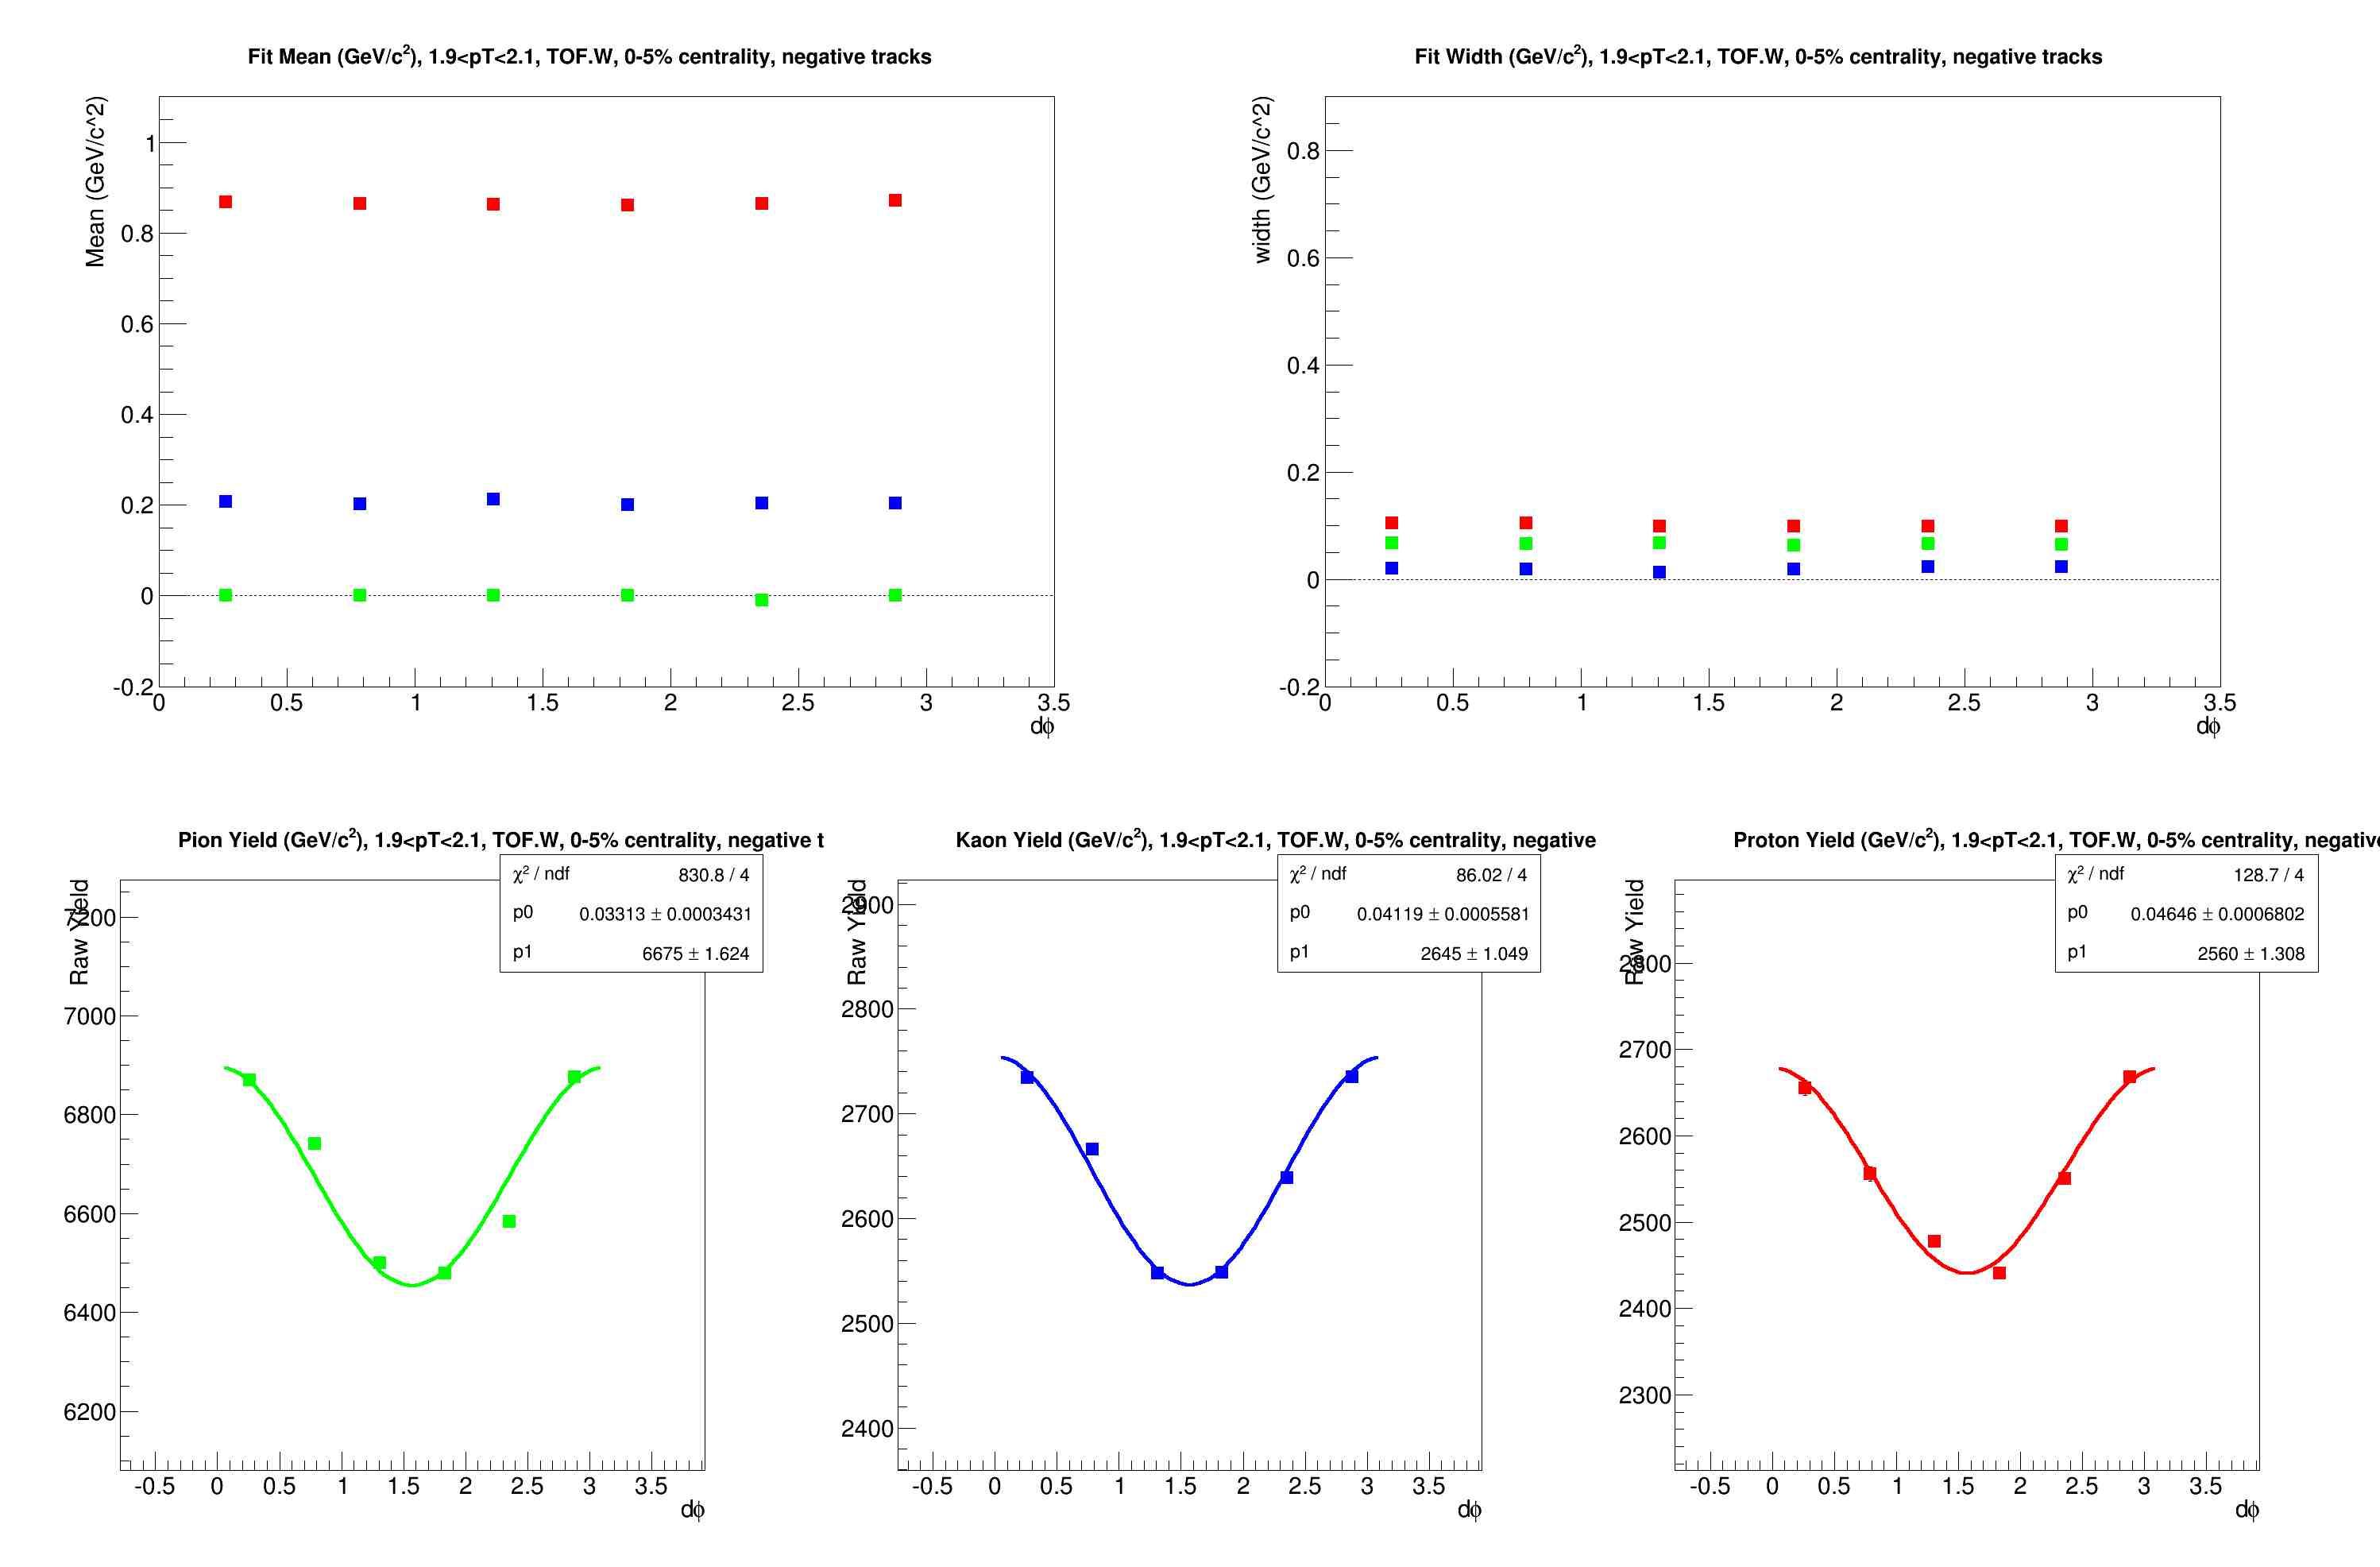
\includegraphics[width=1\textwidth]{lowptfits/fitParams_tof1_cent0_ch0_pT-19-21.jpg}
    \end{subfigure}
    \rule{35em}{0.5pt}
  \caption[PID fits and Yield vs $d\phi$ for $p_T$=1.9-2.1 GeV/c, TOF.W, negative particles ]{$m^2$ Gaussian fits for PID and resulting Yield vs $d\phi$ for $p_T$=1.9-2.1 GeV/c, TOF.W, negative particles}
  \label{fig:fits19-21neg}
\end{figure}

\subsubsection{Mixed Gaussian fits, $p_T$=1.3-2.1 GeV/c, TOF.W, positive charged tracks}

\begin{figure}[H]
  \centering
    \begin{subfigure}[p]{1\textwidth}
    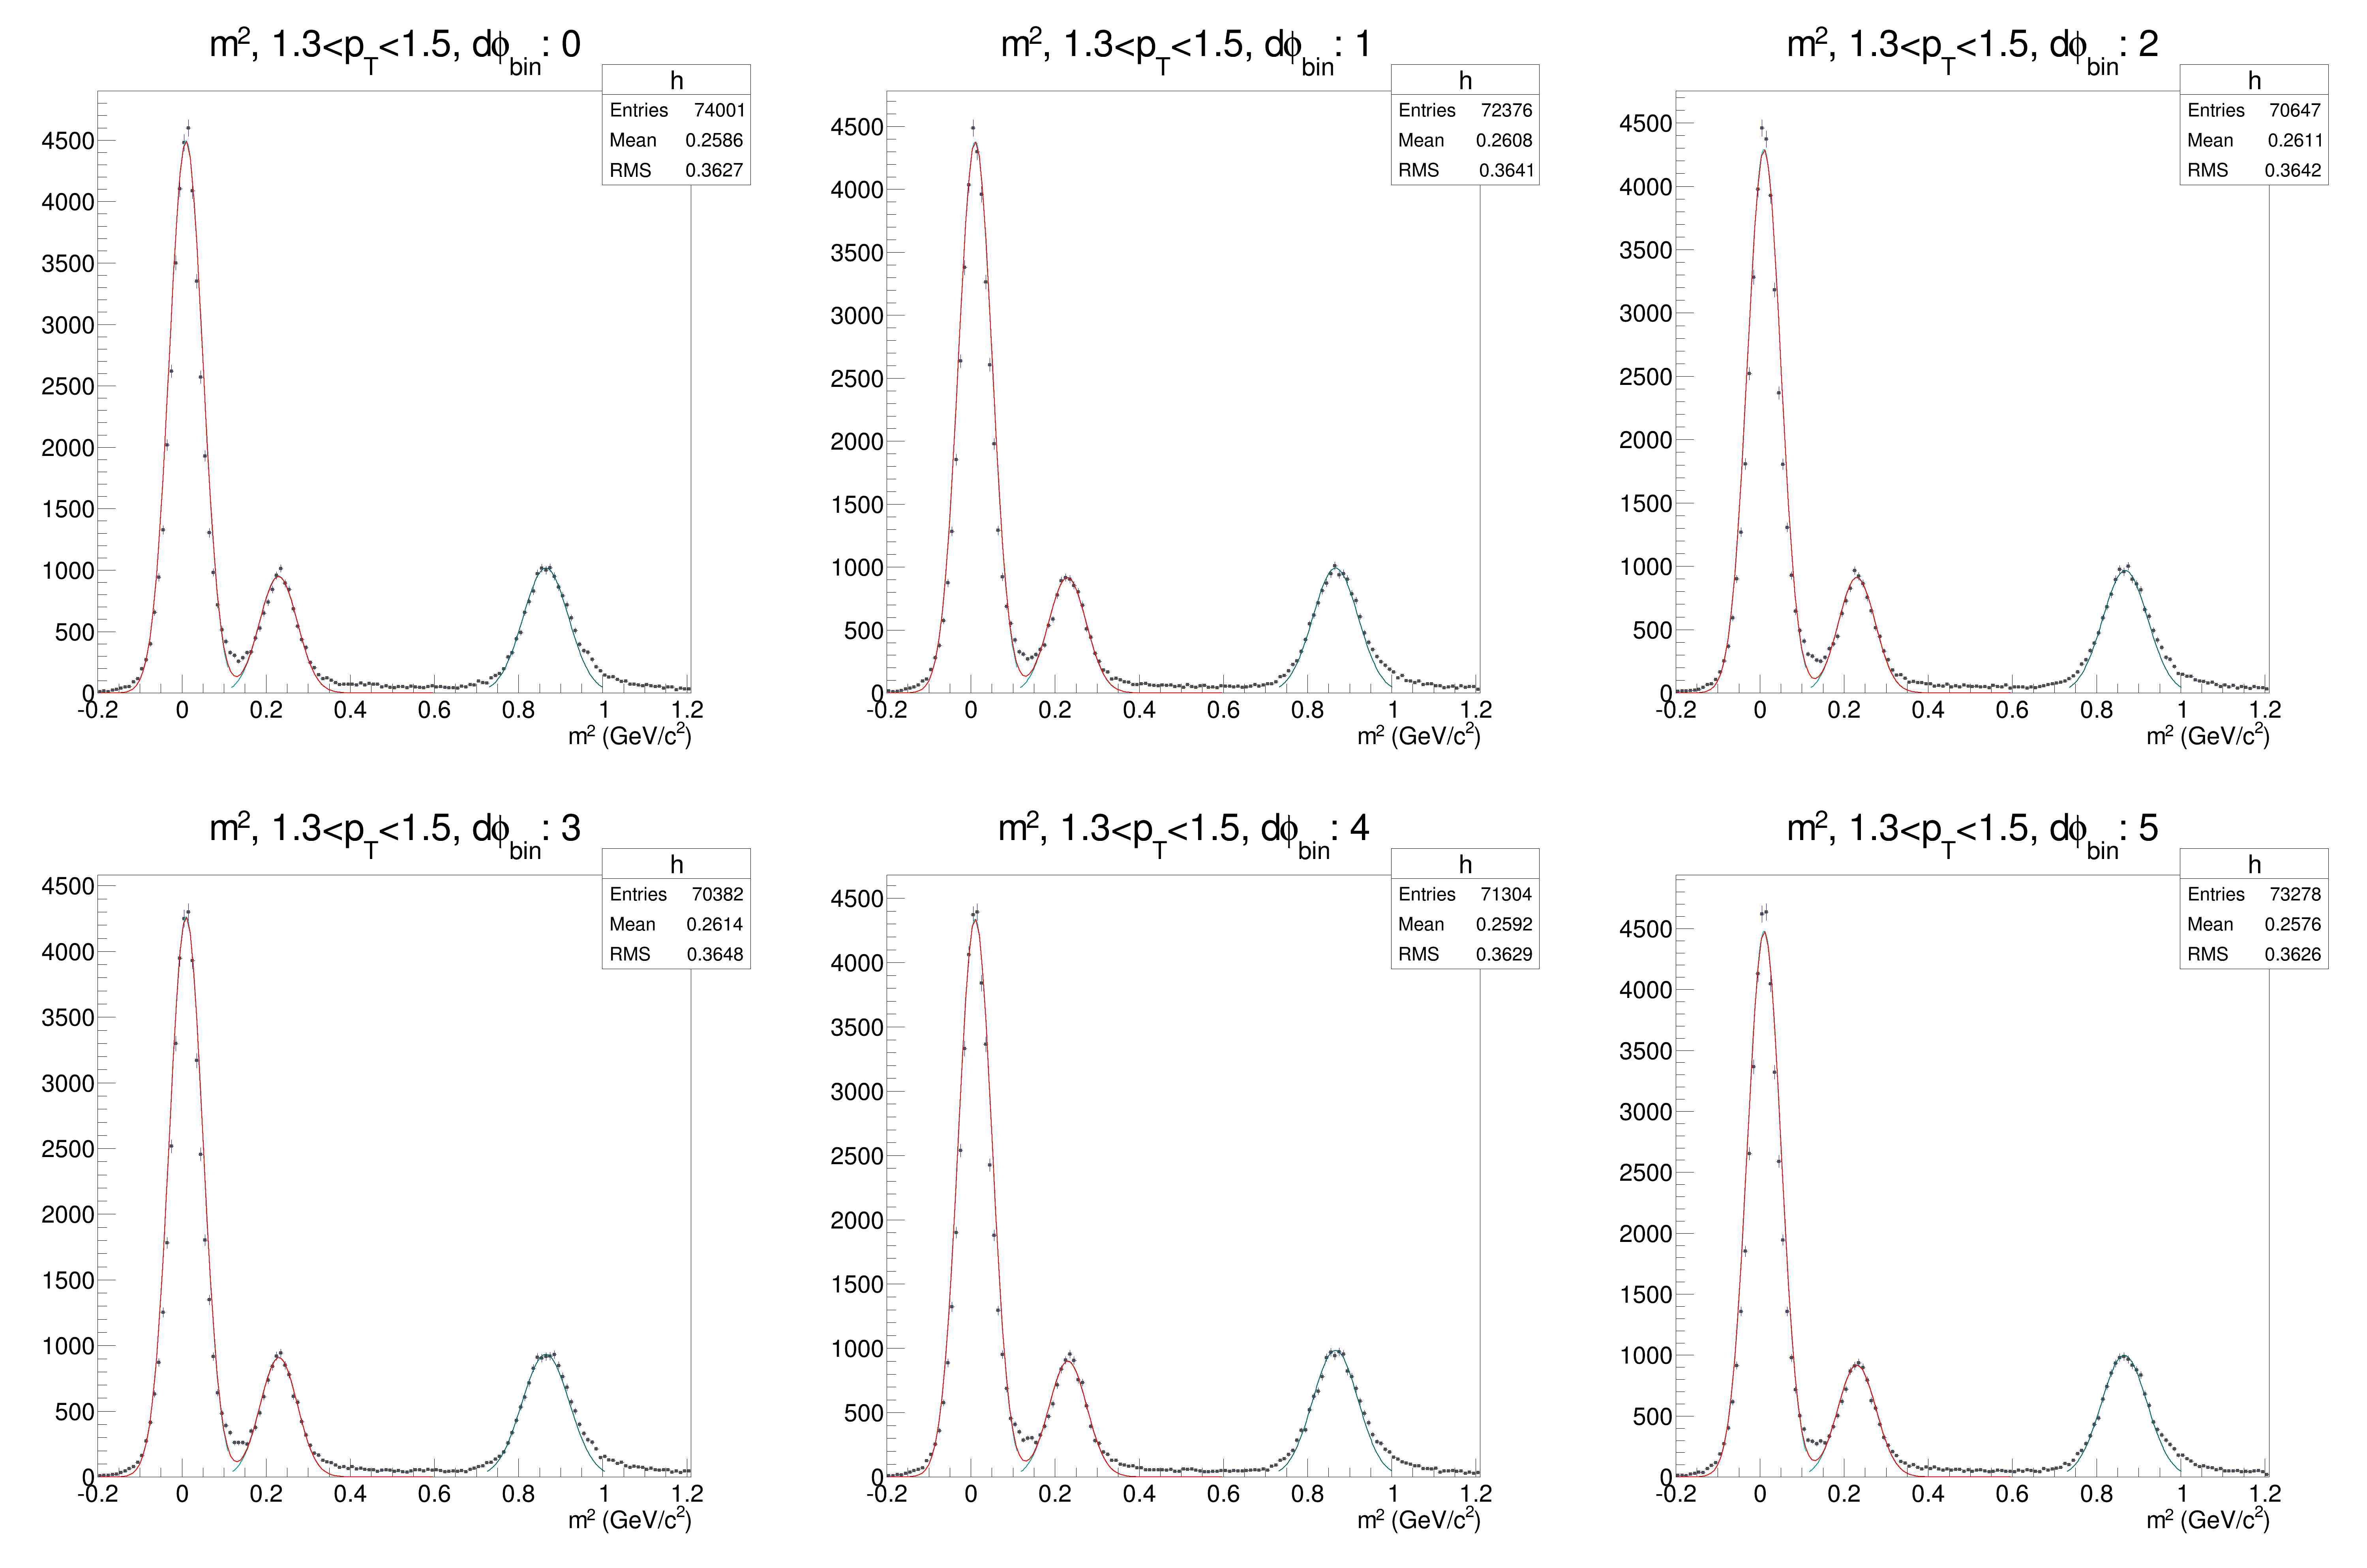
\includegraphics[width=1\textwidth]{lowptfits/yieldvsdphi_tof1_cent0_ch1_pT-13-15.jpg}
    \end{subfigure}
    \begin{subfigure}[p]{1\textwidth}
    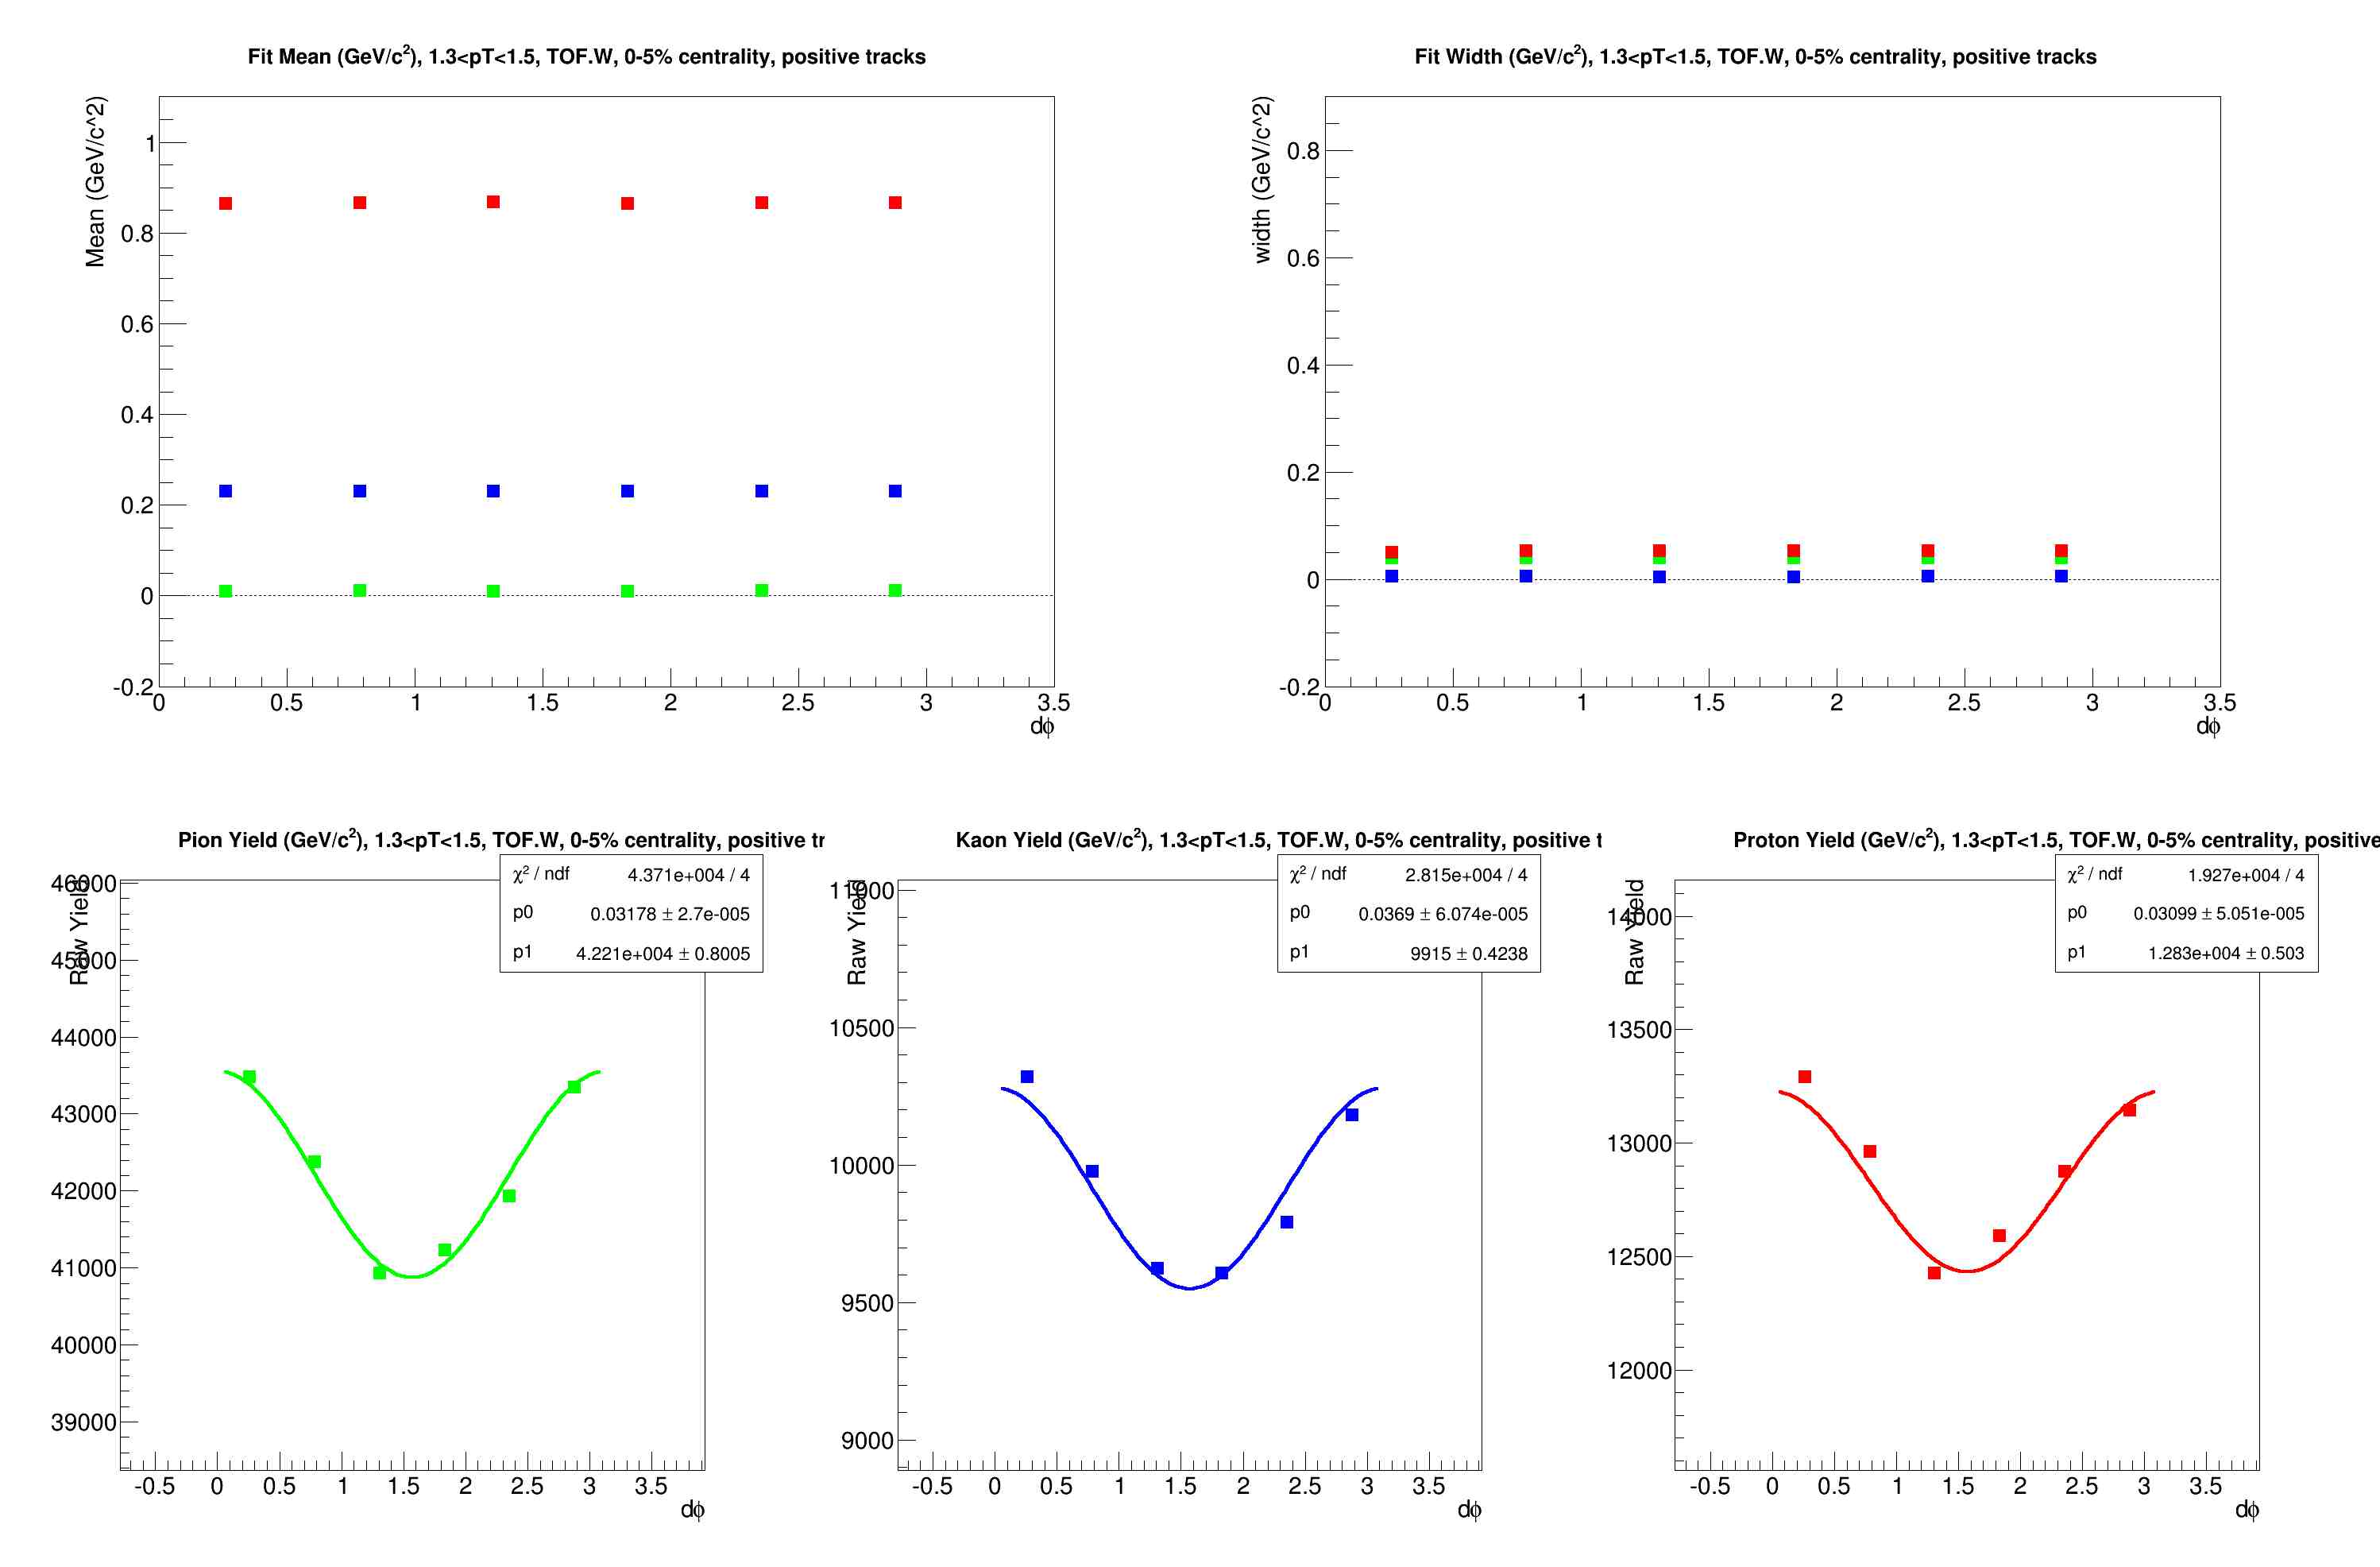
\includegraphics[width=1\textwidth]{lowptfits/fitParams_tof1_cent0_ch1_pT-13-15.jpg}
    \end{subfigure}
    \rule{35em}{0.5pt}
  \caption[PID fits and Yield vs $d\phi$ for $p_T$=1.3-1.5 GeV/c, TOF.W, positive particles ]{$m^2$ Gaussian fits for PID and resulting Yield vs $d\phi$ for $p_T$=1.3-1.5 GeV/c, TOF.W, positive particles}
  \label{fig:fits13-15pos}
\end{figure}

\begin{figure}[H]
  \centering
    \begin{subfigure}[p]{1\textwidth}
    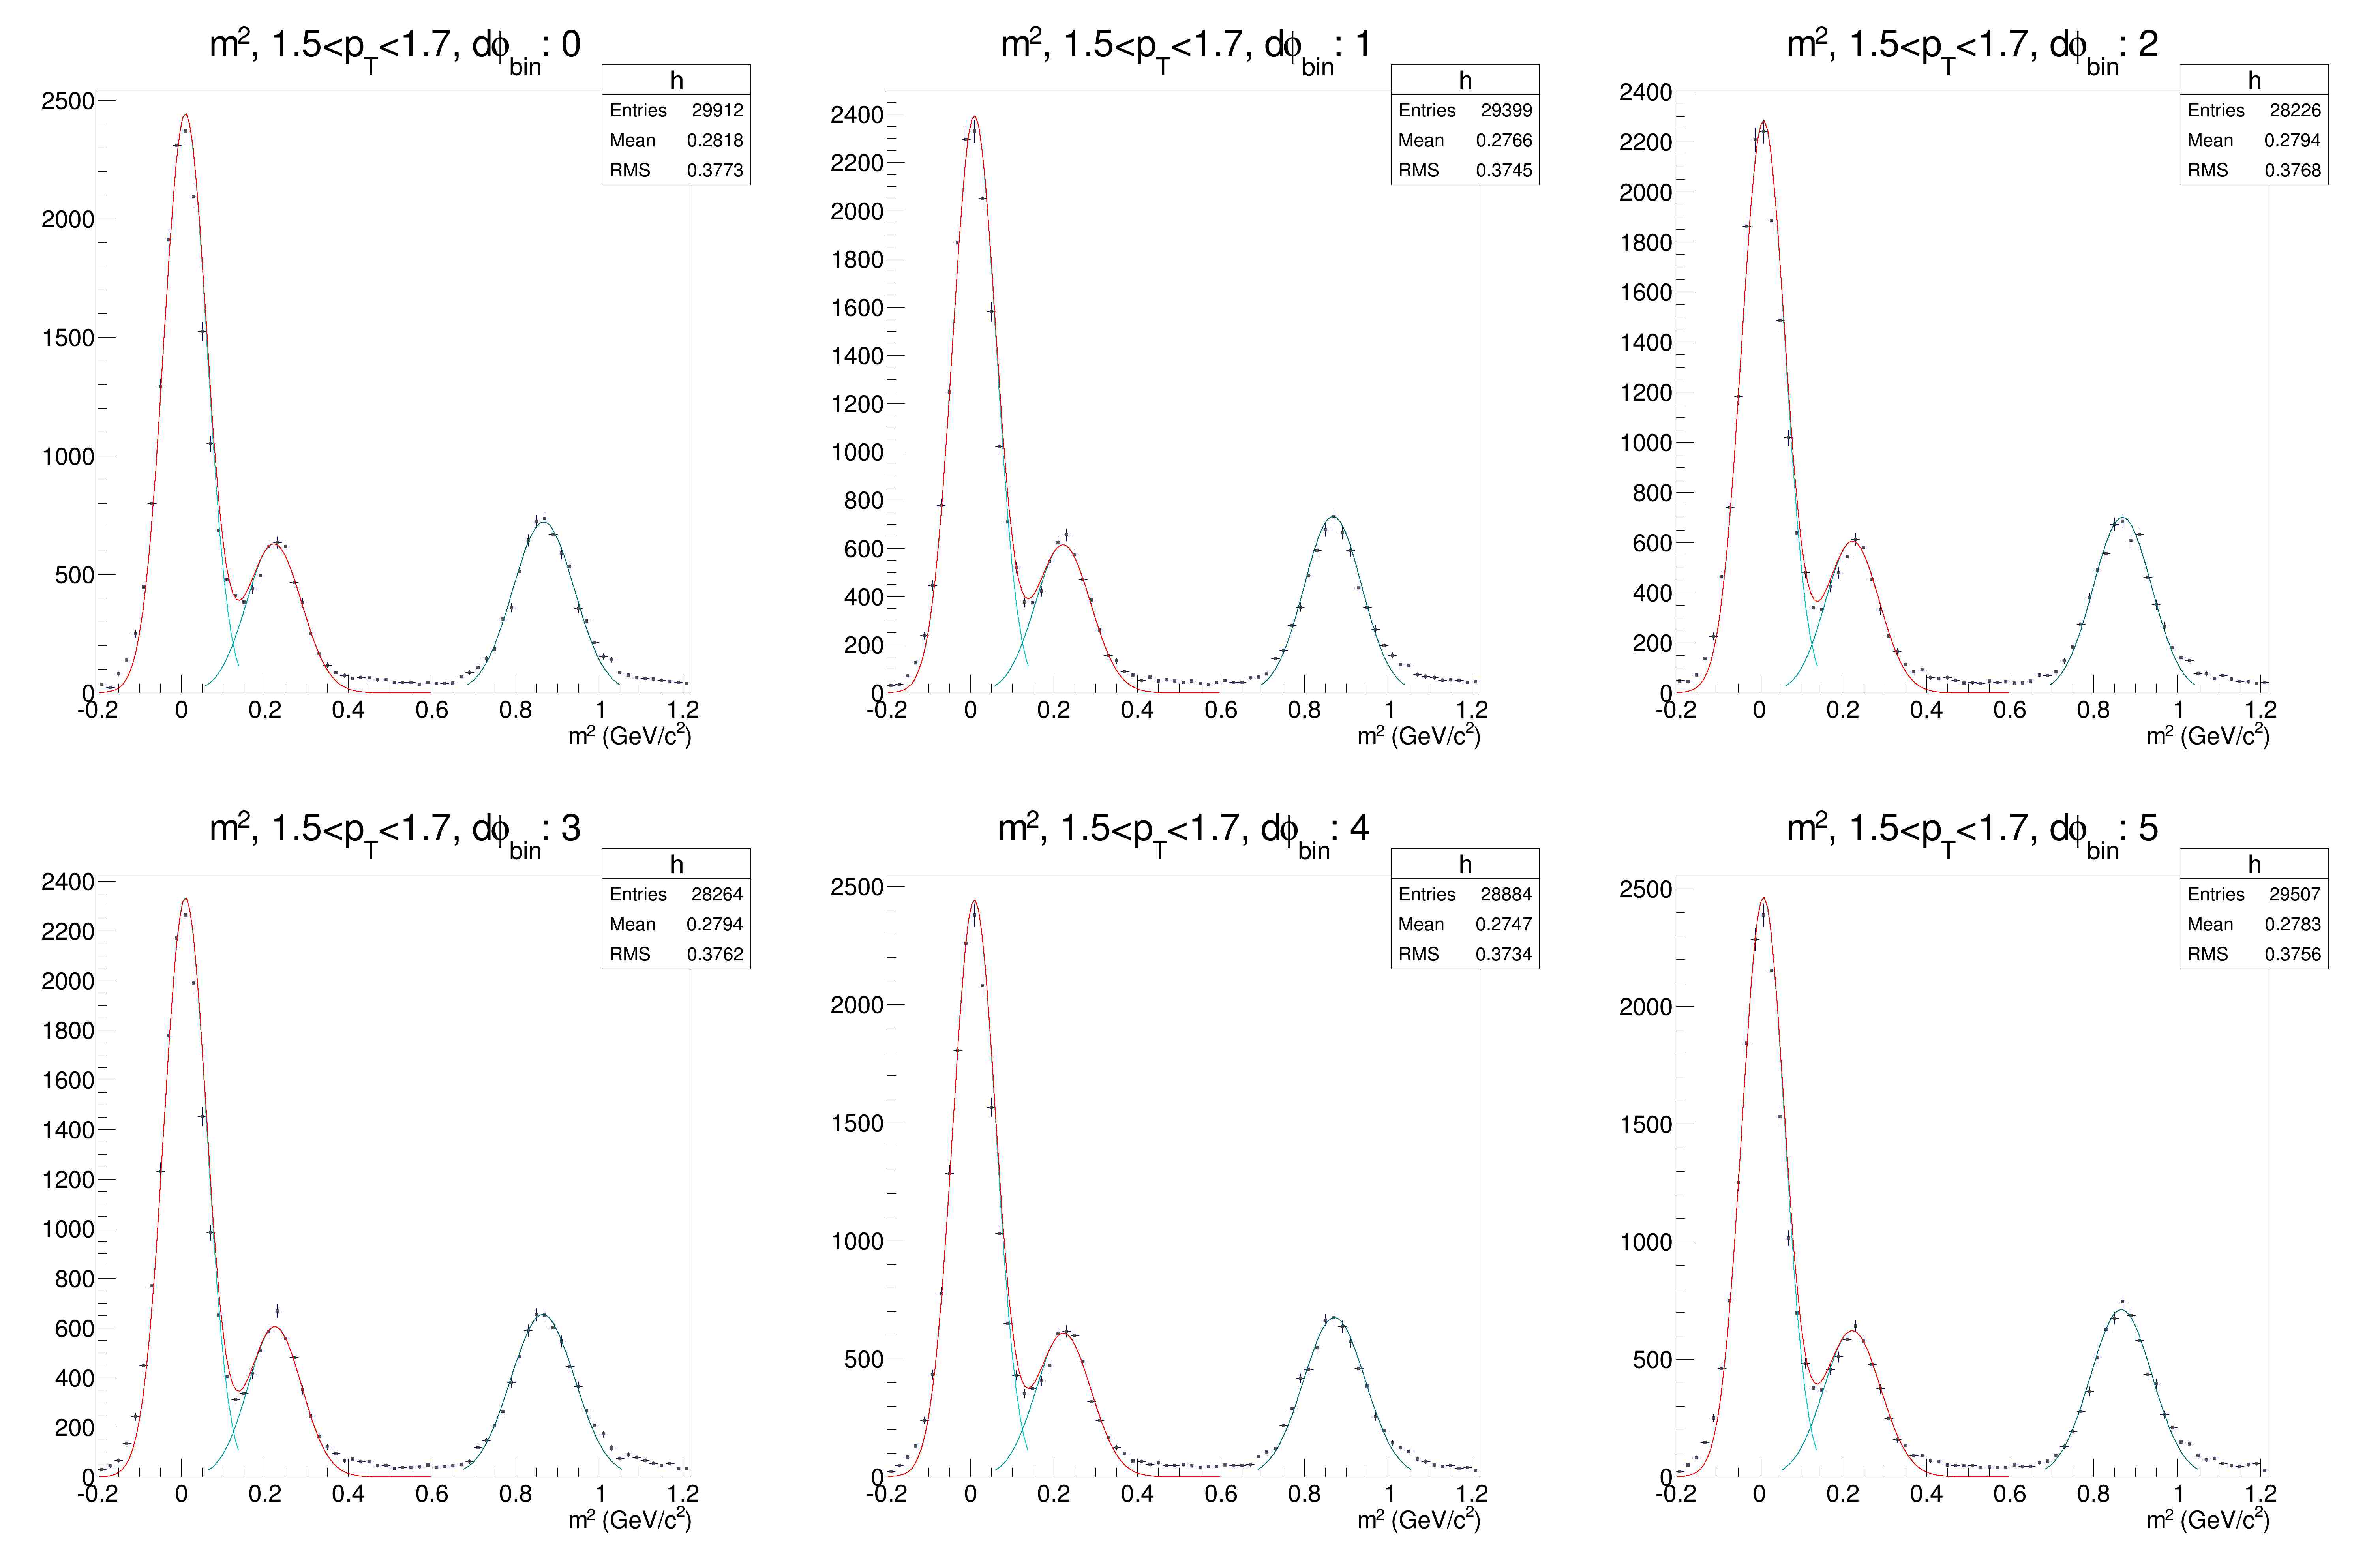
\includegraphics[width=1\textwidth]{lowptfits/yieldvsdphi_tof1_cent0_ch1_pT-15-17.jpg}
    \end{subfigure}
    \begin{subfigure}[p]{1\textwidth}
    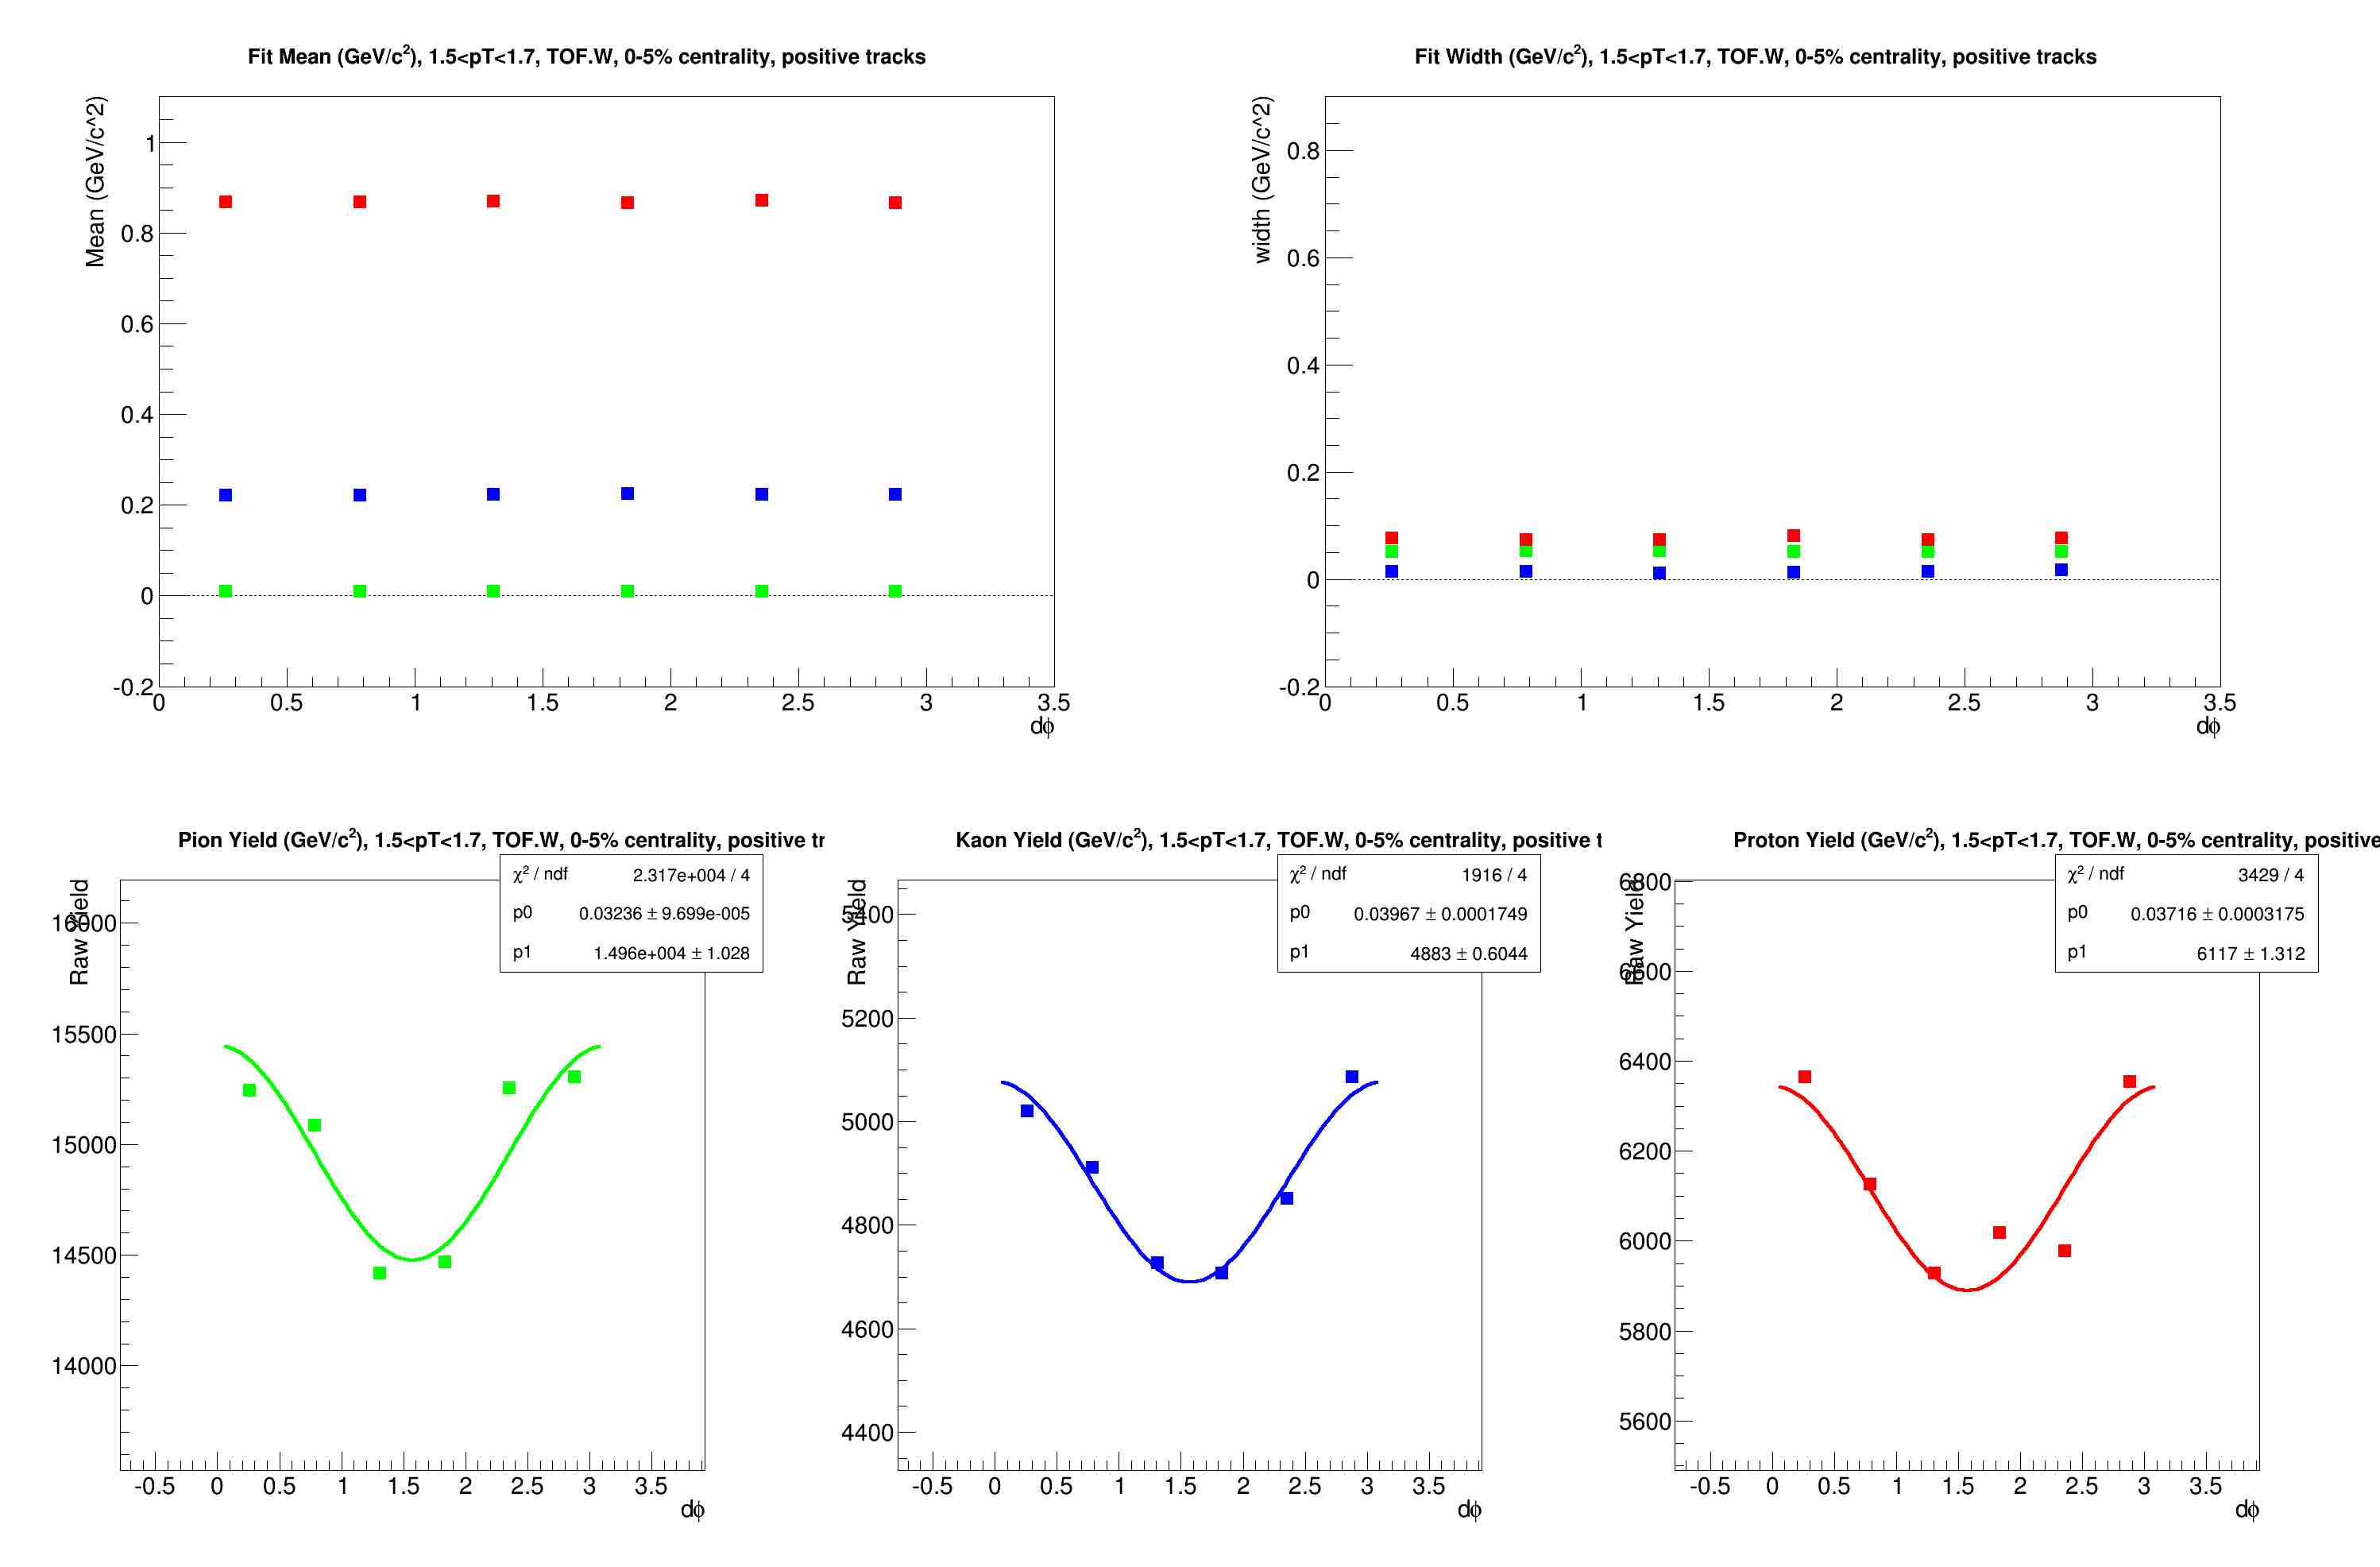
\includegraphics[width=1\textwidth]{lowptfits/fitParams_tof1_cent0_ch1_pT-15-17.jpg}
    \end{subfigure}
    \rule{35em}{0.5pt}
  \caption[PID fits and Yield vs $d\phi$ for $p_T$=1.5-1.7 GeV/c, TOF.W, positive particles ]{$m^2$ Gaussian fits for PID and resulting Yield vs $d\phi$ for $p_T$=1.5-1.7 GeV/c, TOF.W, positive particles}
  \label{fig:fits15-17pos}
\end{figure}

\begin{figure}[H]
  \centering
    \begin{subfigure}[p]{1\textwidth}
    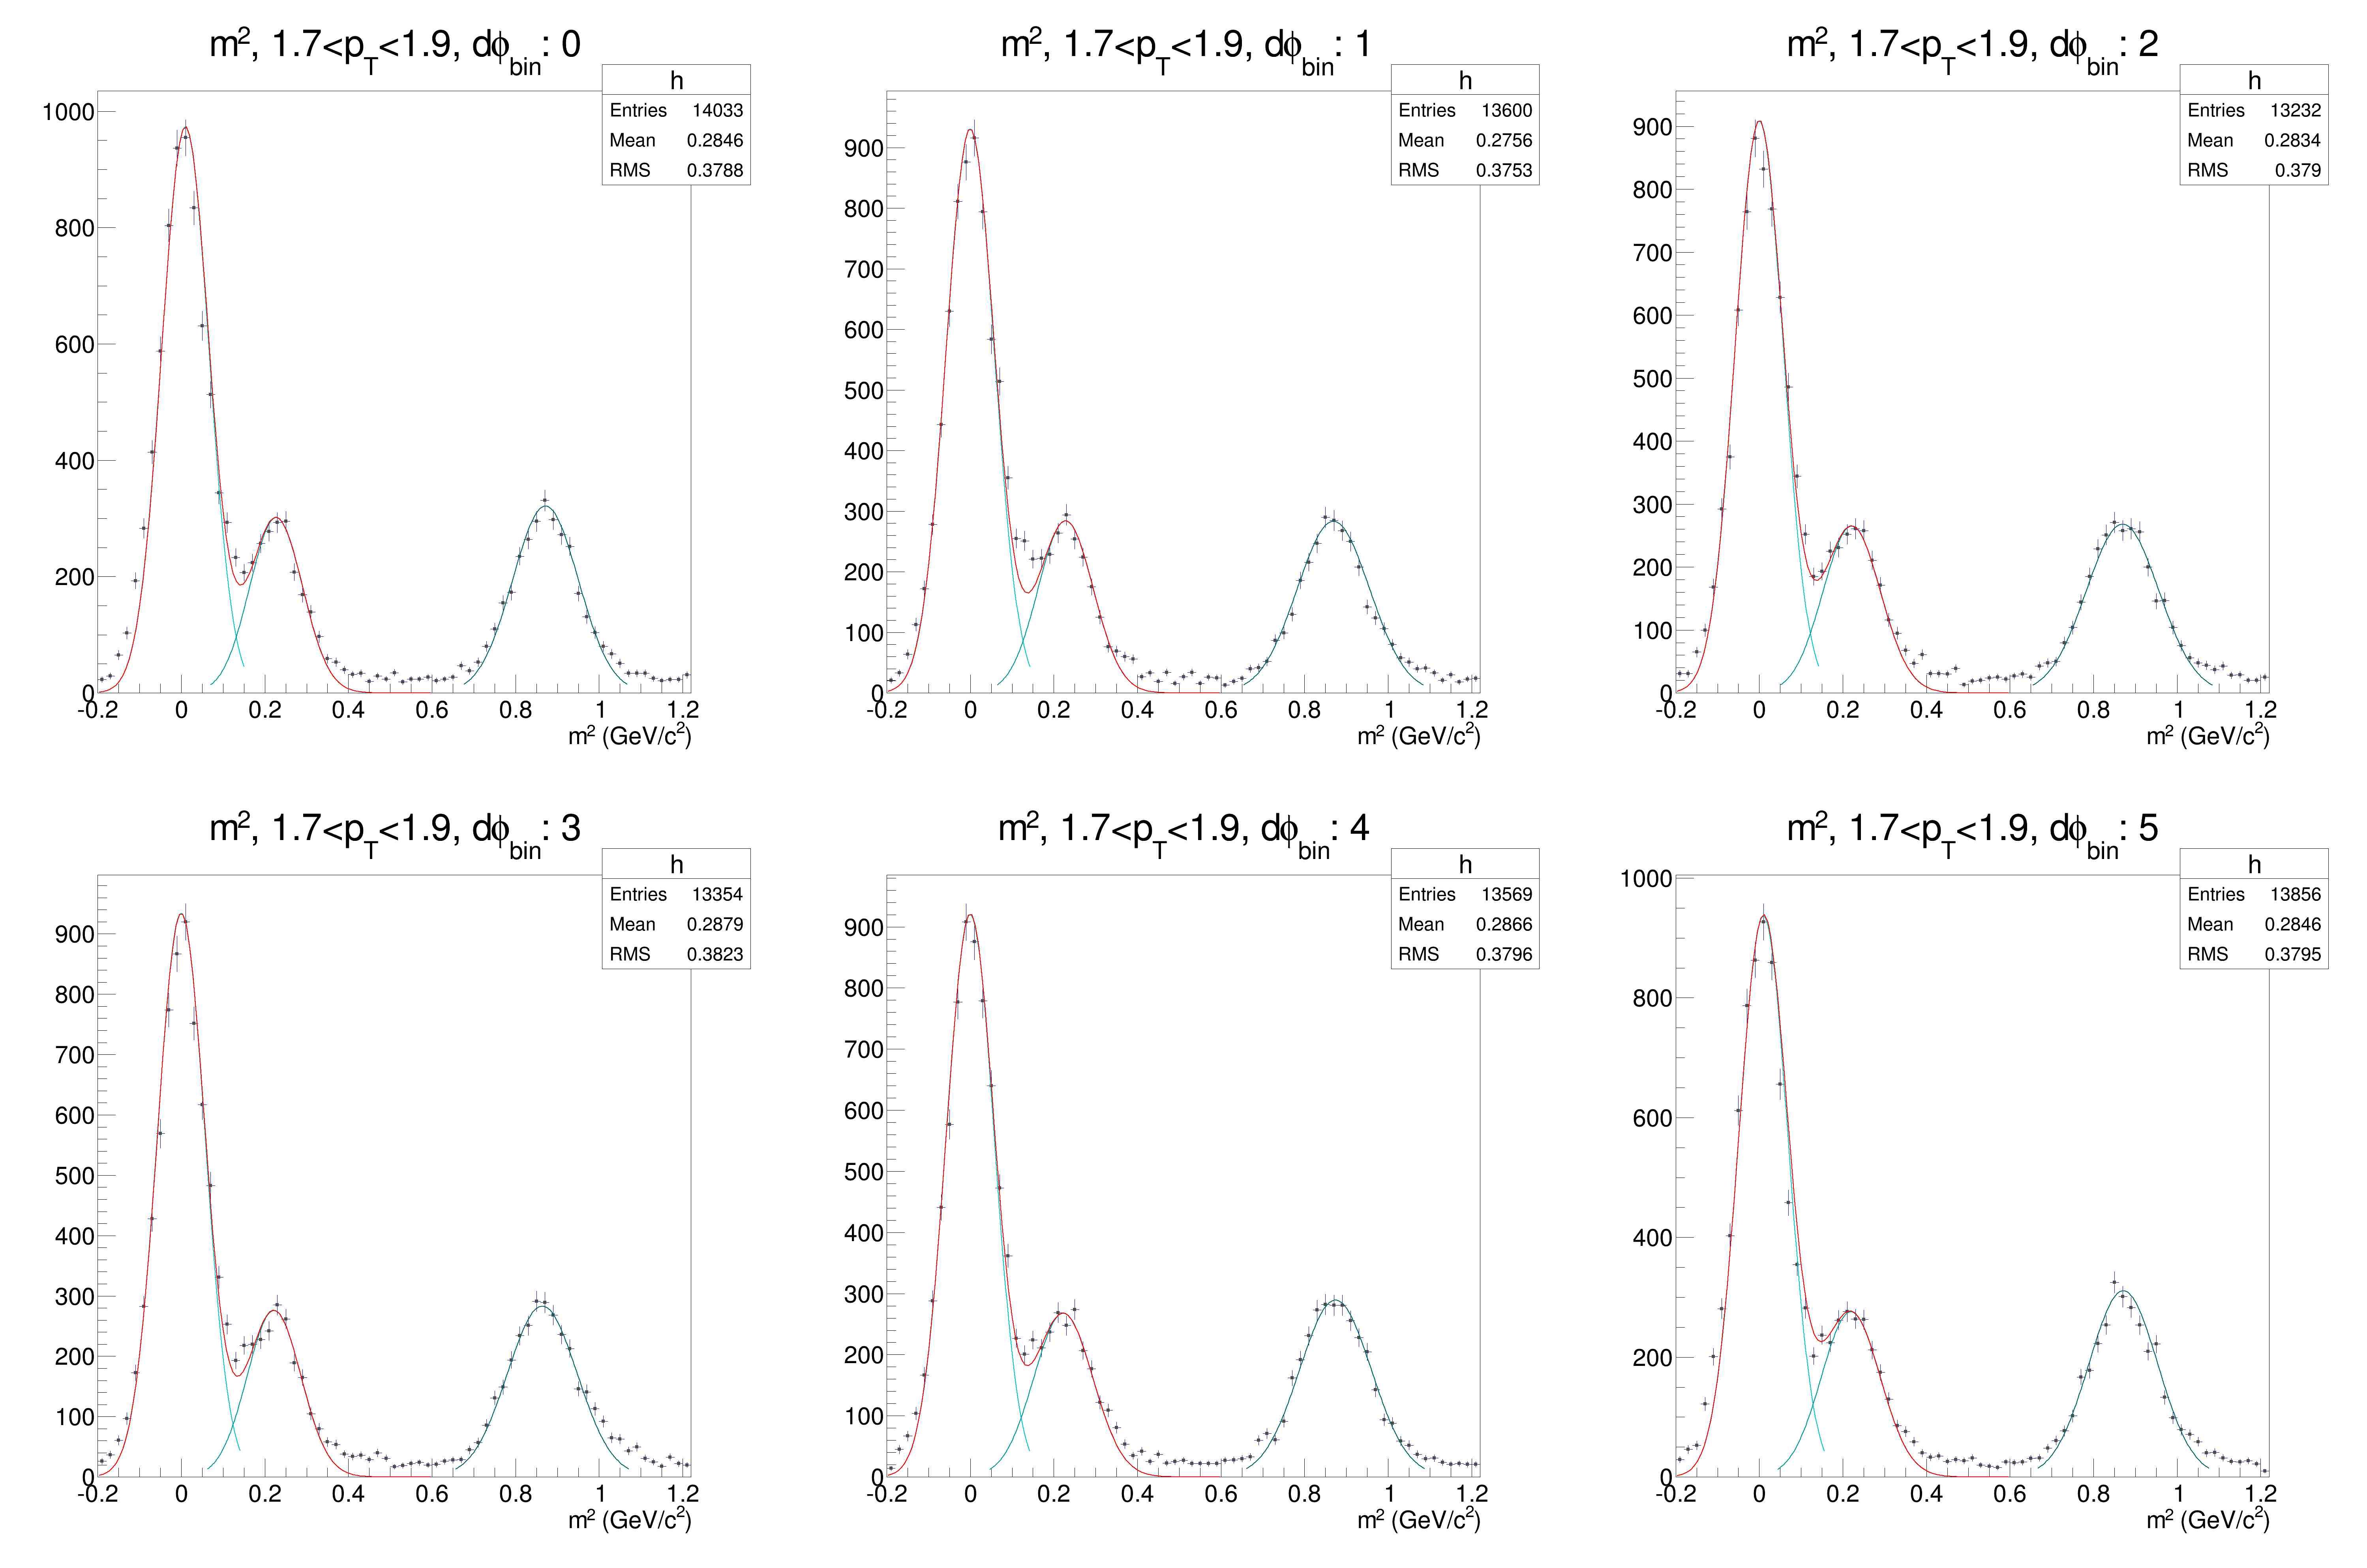
\includegraphics[width=1\textwidth]{lowptfits/yieldvsdphi_tof1_cent0_ch1_pT-17-19.jpg}
    \end{subfigure}
    \begin{subfigure}[p]{1\textwidth}
    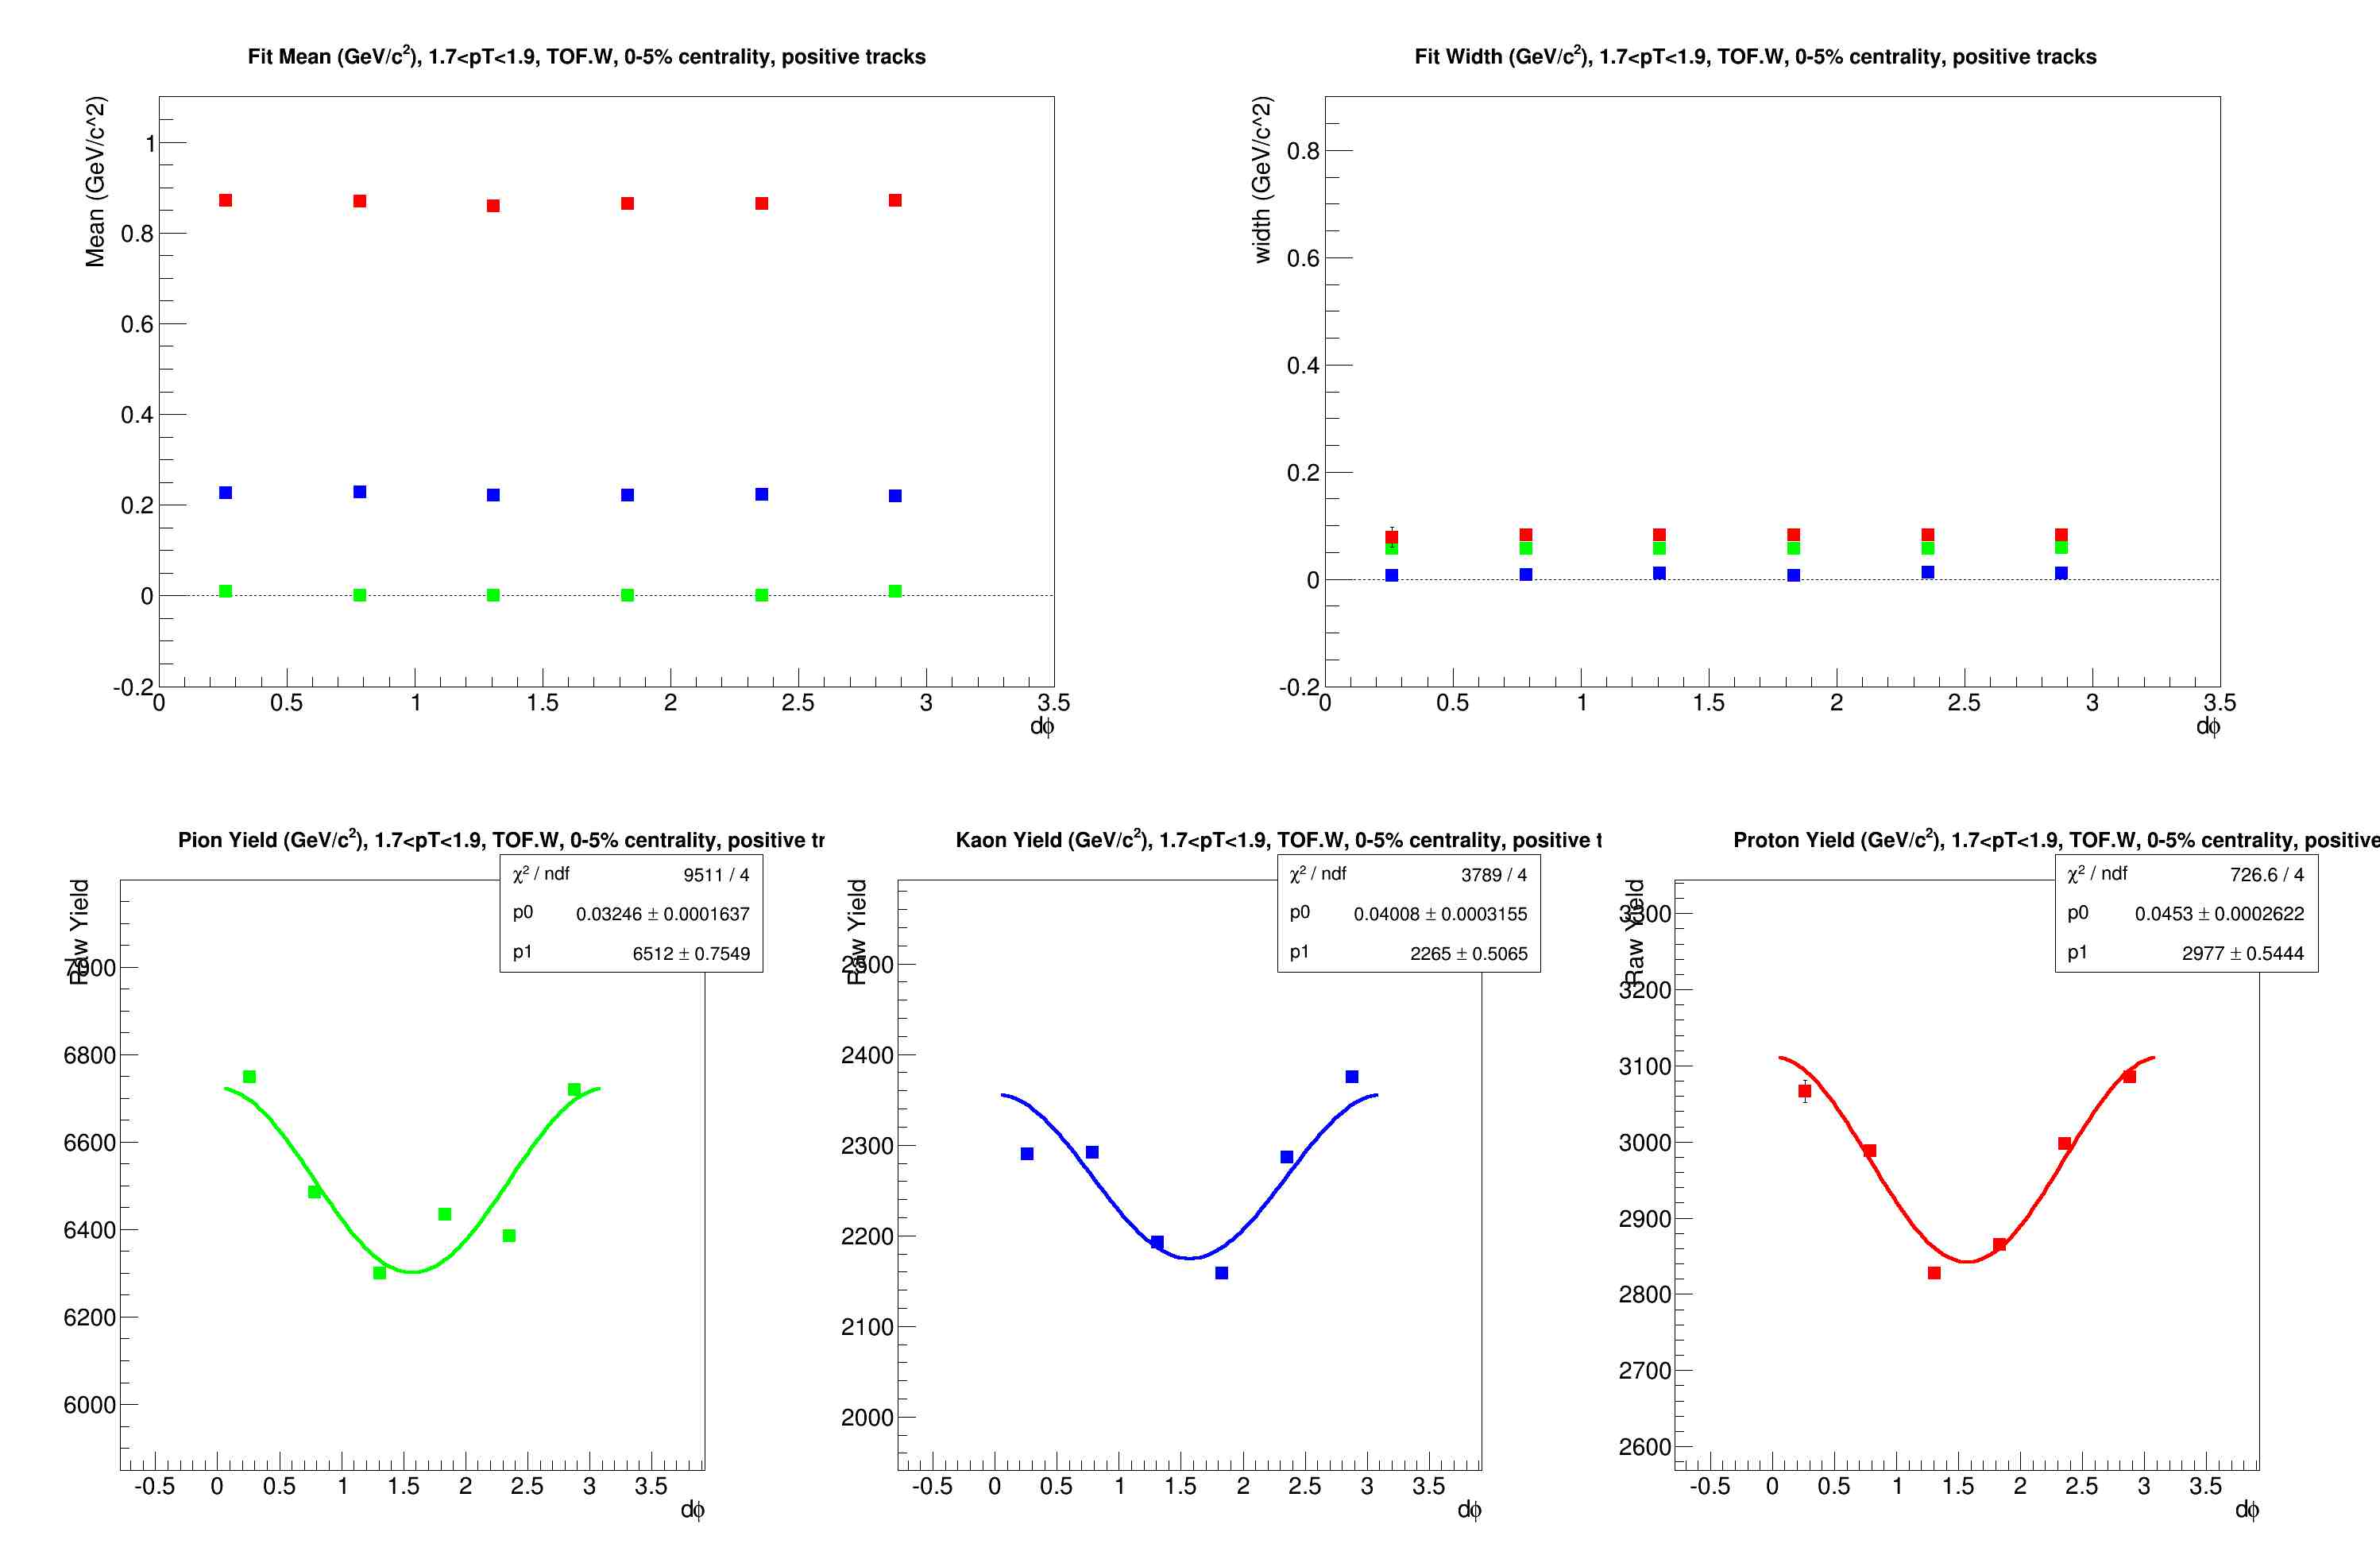
\includegraphics[width=1\textwidth]{lowptfits/fitParams_tof1_cent0_ch1_pT-17-19.jpg}
    \end{subfigure}
    \rule{35em}{0.5pt}
  \caption[PID fits and Yield vs $d\phi$ for $p_T$=1.7-1.9 GeV/c, TOF.W, positive particles ]{$m^2$ Gaussian fits for PID and resulting Yield vs $d\phi$ for $p_T$=1.7-1.9 GeV/c, TOF.W, positive particles}
  \label{fig:fits17-19pos}
\end{figure}

\begin{figure}[H]
  \centering
    \begin{subfigure}[p]{1\textwidth}
    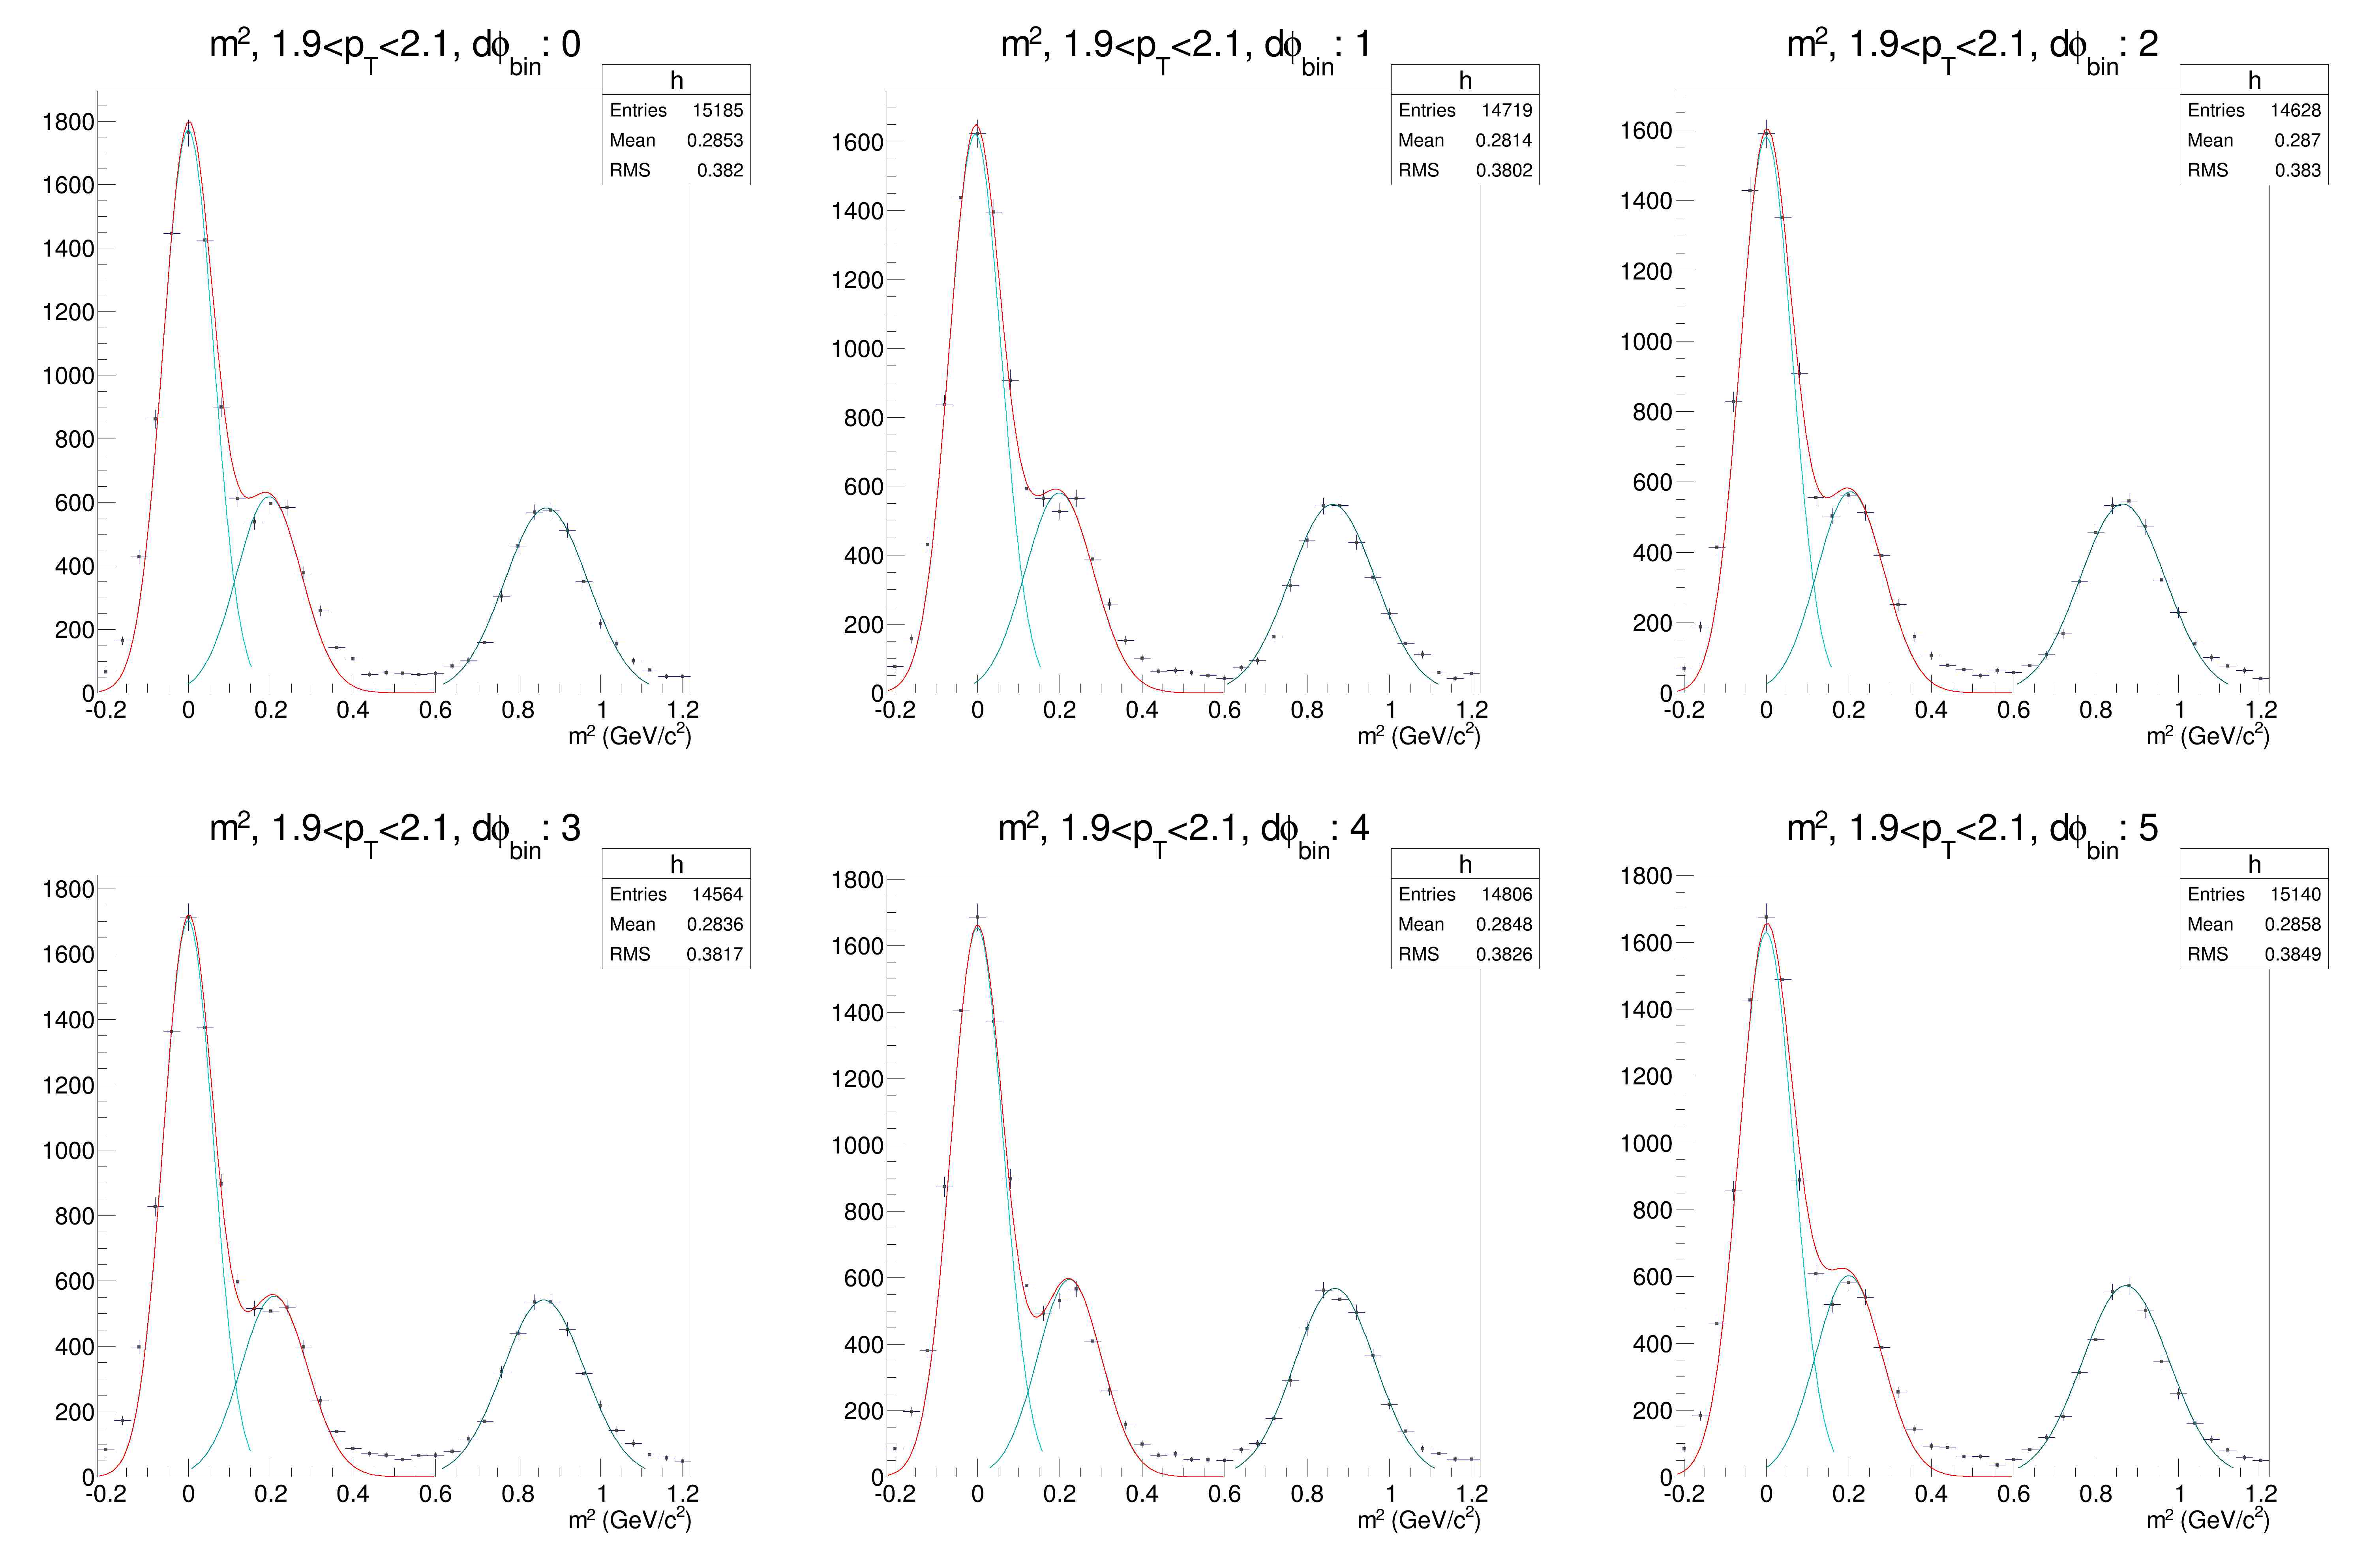
\includegraphics[width=1\textwidth]{lowptfits/yieldvsdphi_tof1_cent0_ch1_pT-19-21.jpg}
    \end{subfigure}
    \begin{subfigure}[p]{1\textwidth}
    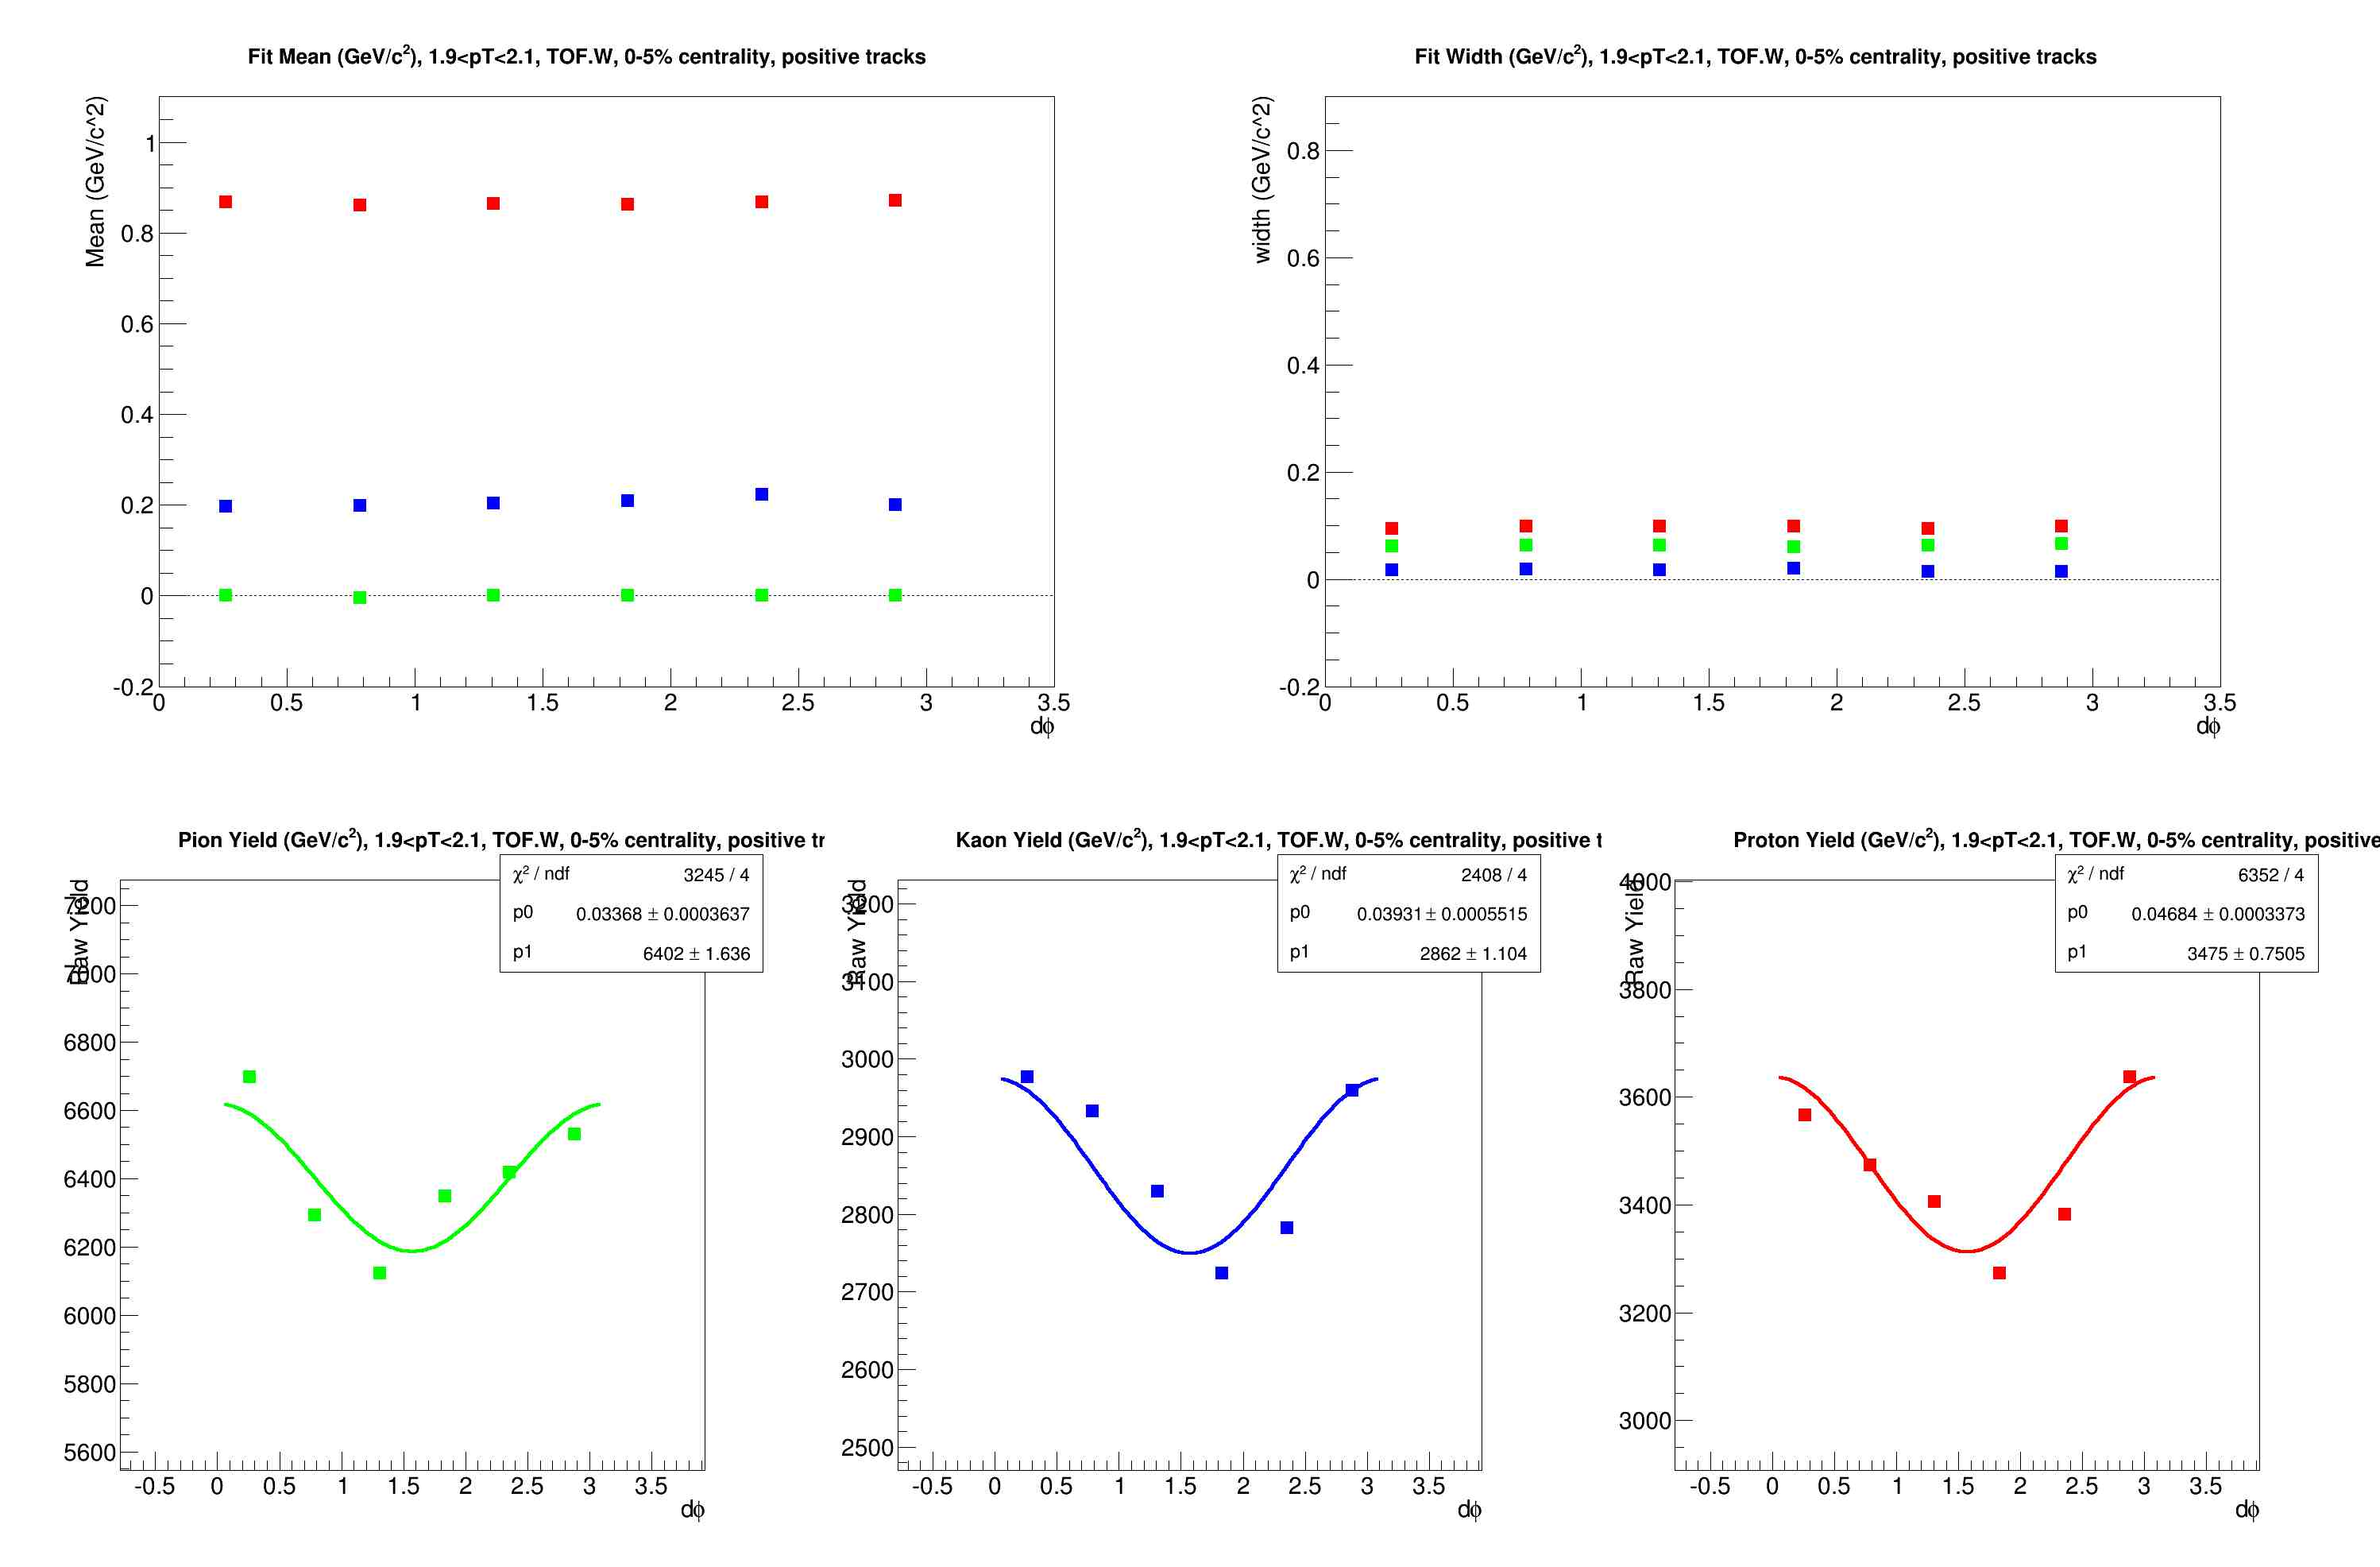
\includegraphics[width=1\textwidth]{lowptfits/fitParams_tof1_cent0_ch1_pT-19-21.jpg}
    \end{subfigure}
    \rule{35em}{0.5pt}
  \caption[PID fits and Yield vs $d\phi$ for $p_T$=1.9-2.1 GeV/c, TOF.W, positive particles ]{$m^2$ Gaussian fits for PID and resulting Yield vs $d\phi$ for $p_T$=1.9-2.1 GeV/c, TOF.W, positive particles}
  \label{fig:fits19-21pos}
\end{figure}

\subsection{TOF.W and ACC, $p_T$=2.1-3.5 GeV, negative charged tracks}
\label{app:accdata}
\begin{figure}[H]
  \centering
    \begin{subfigure}{1\textwidth}
    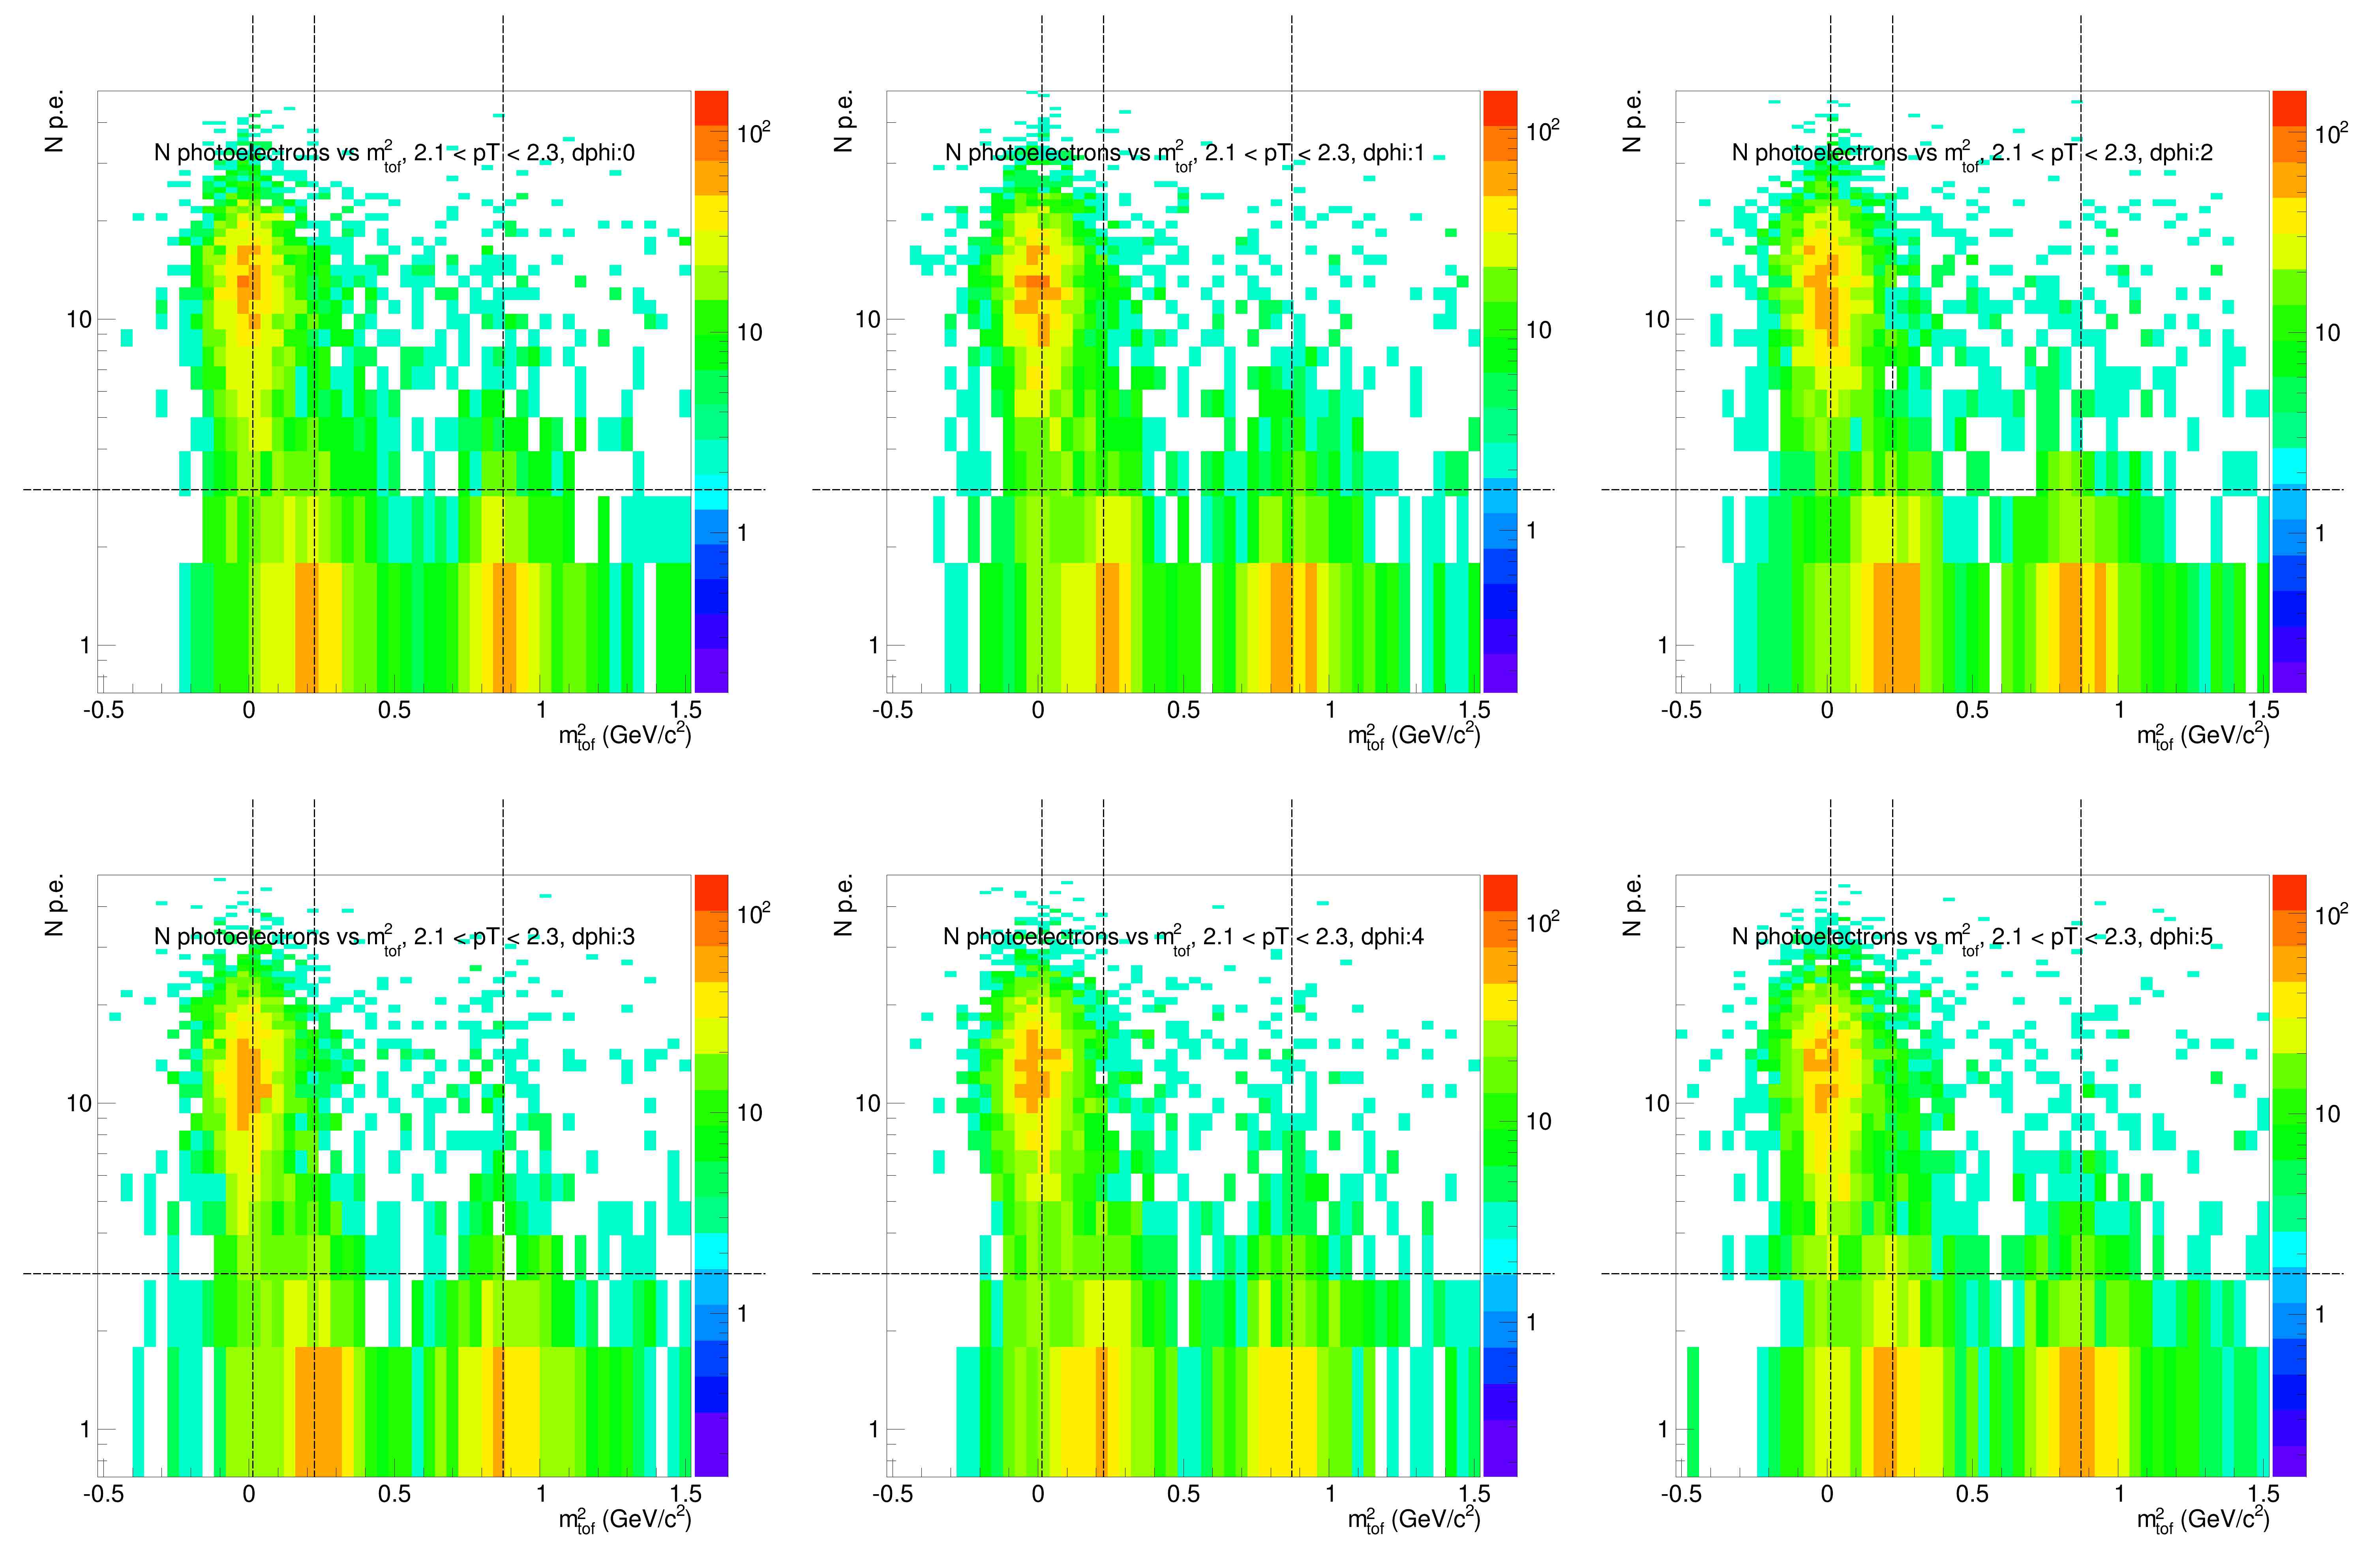
\includegraphics[width=1\textwidth]{hiptfits/neg/PSaccthreshold_cent0_ich0_accfire0_ptbin8.jpg}
    \caption{$N_{p.e.}$ vs $m^2$}
    \end{subfigure}
\end{figure}
\begin{figure}[H]
  \ContinuedFloat
    \begin{subfigure}{1\textwidth}
    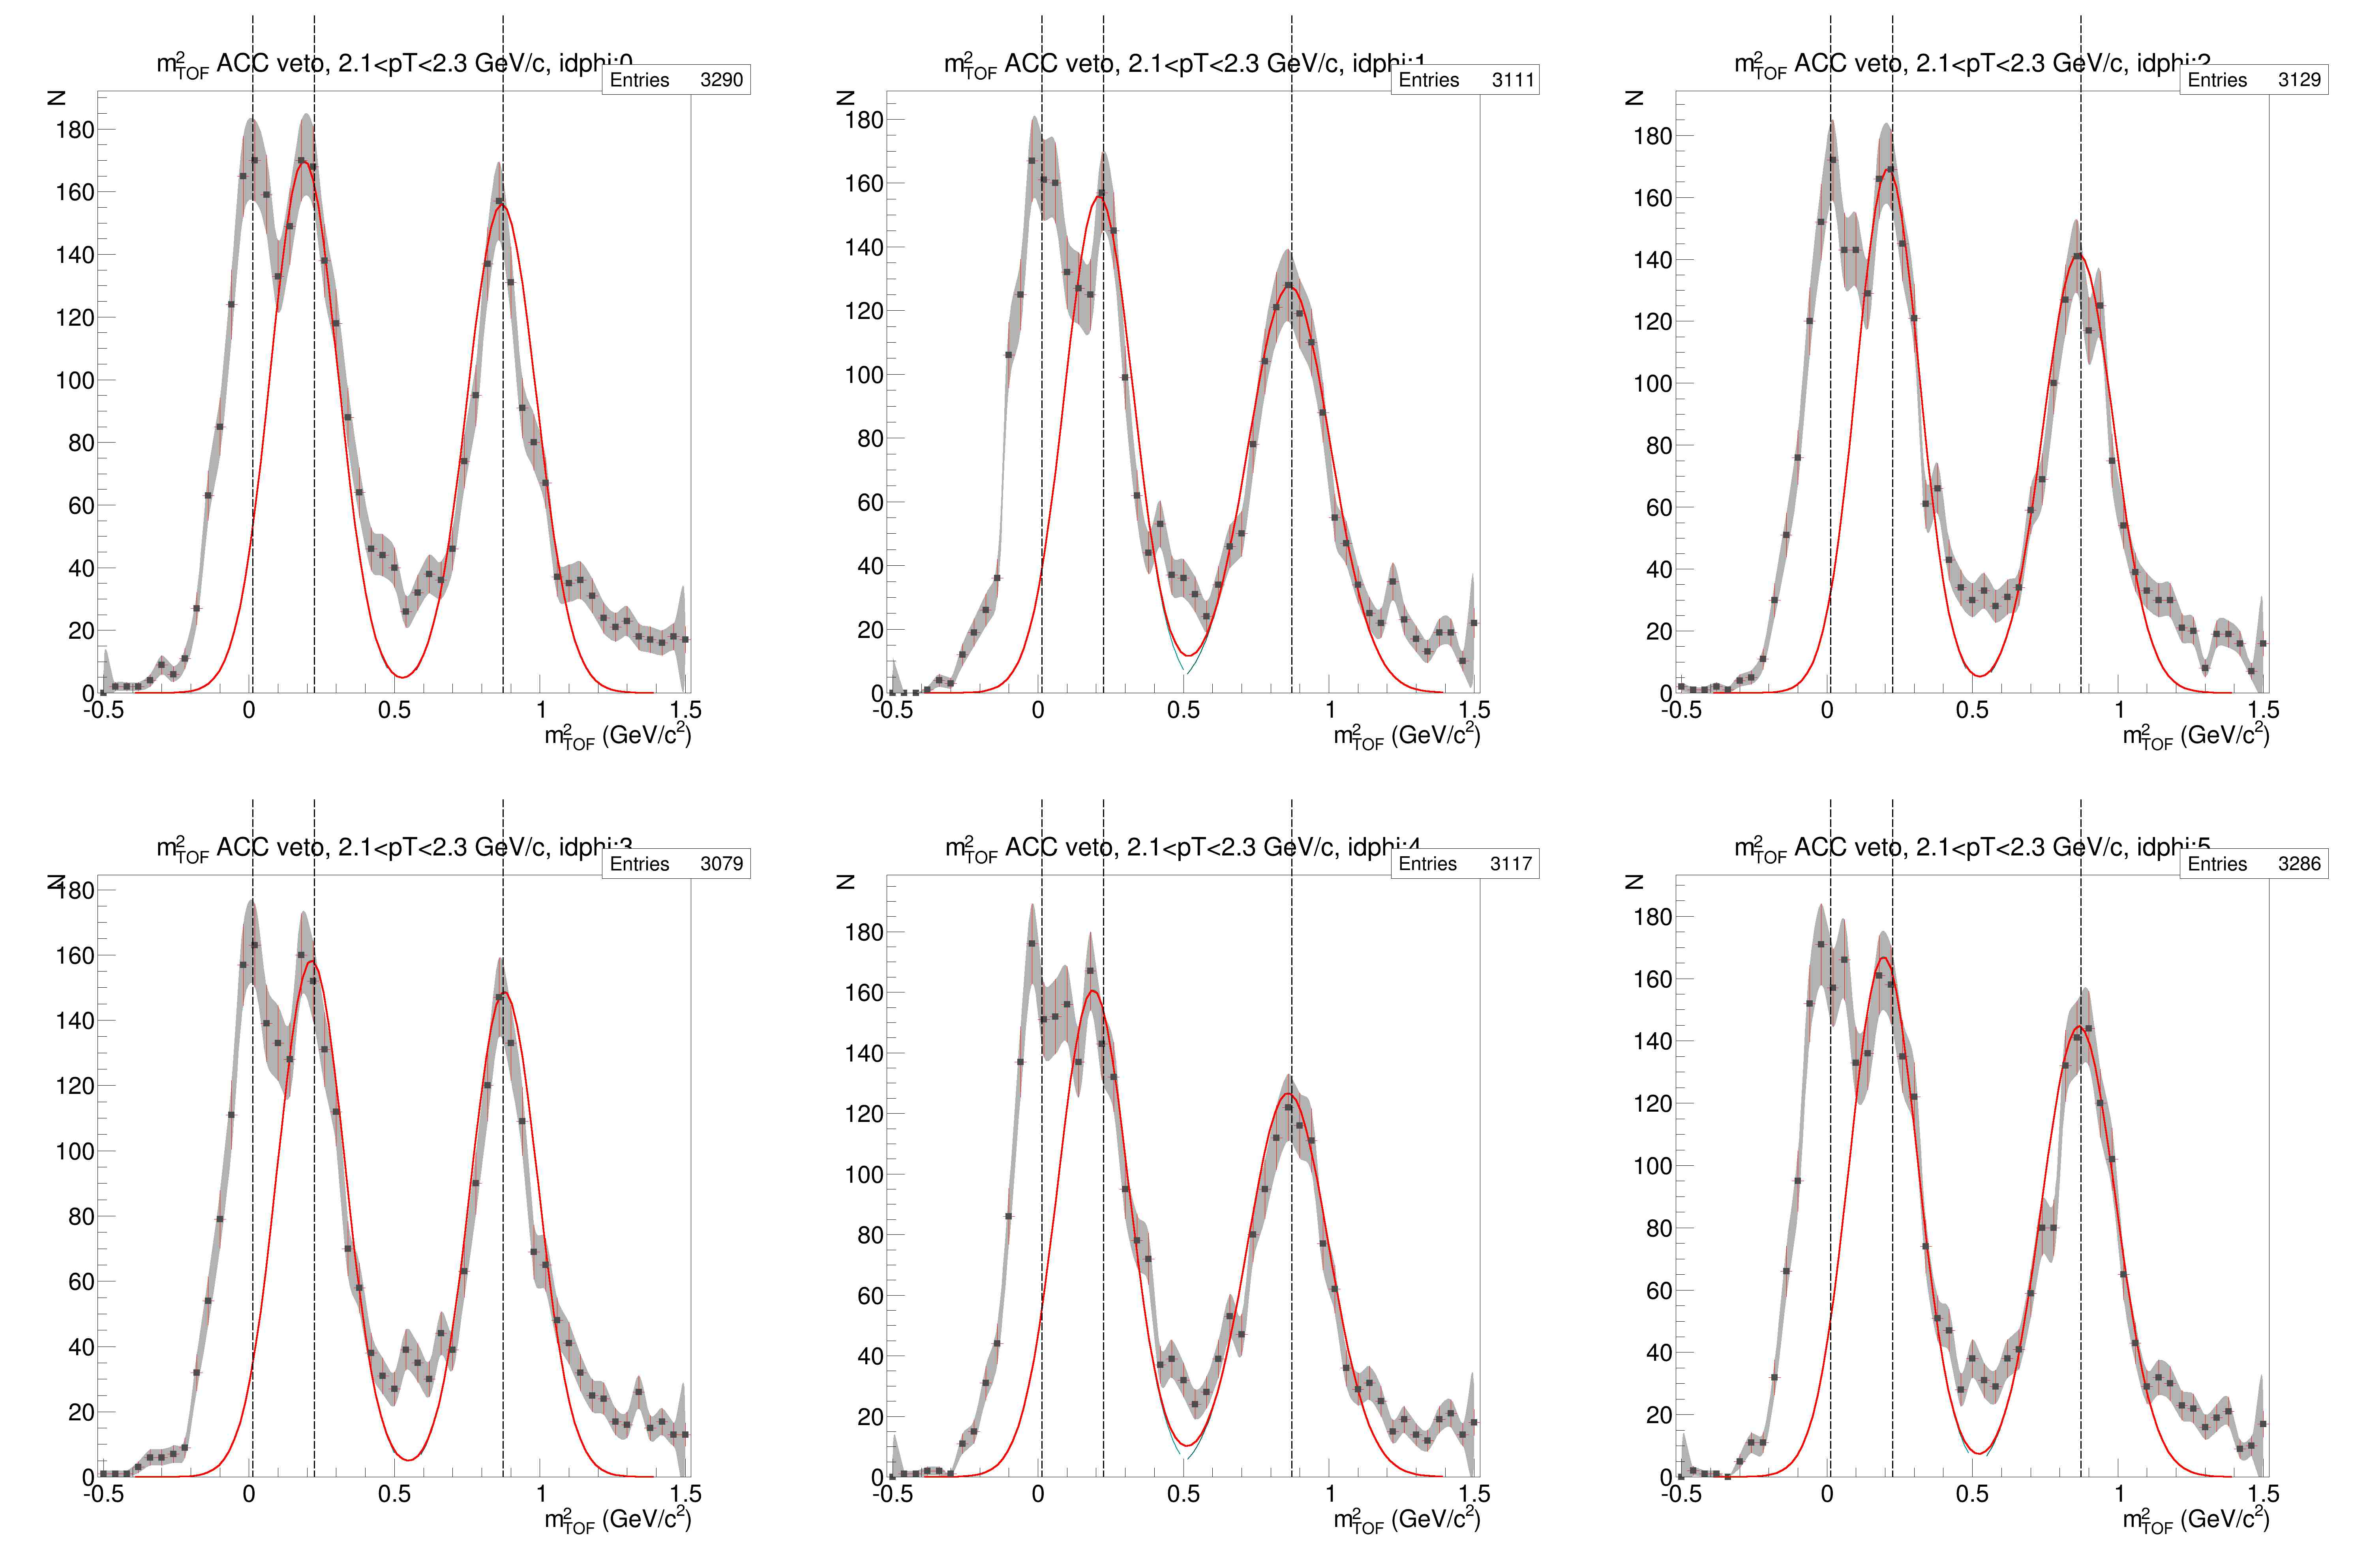
\includegraphics[width=1\textwidth]{hiptfits/neg/PSm2_cent0_ich0_accfire0_ptbin8.jpg}
    \caption{$m^2$ for ACC vetoed tracks}
    \end{subfigure}
    \begin{subfigure}{1\textwidth}
    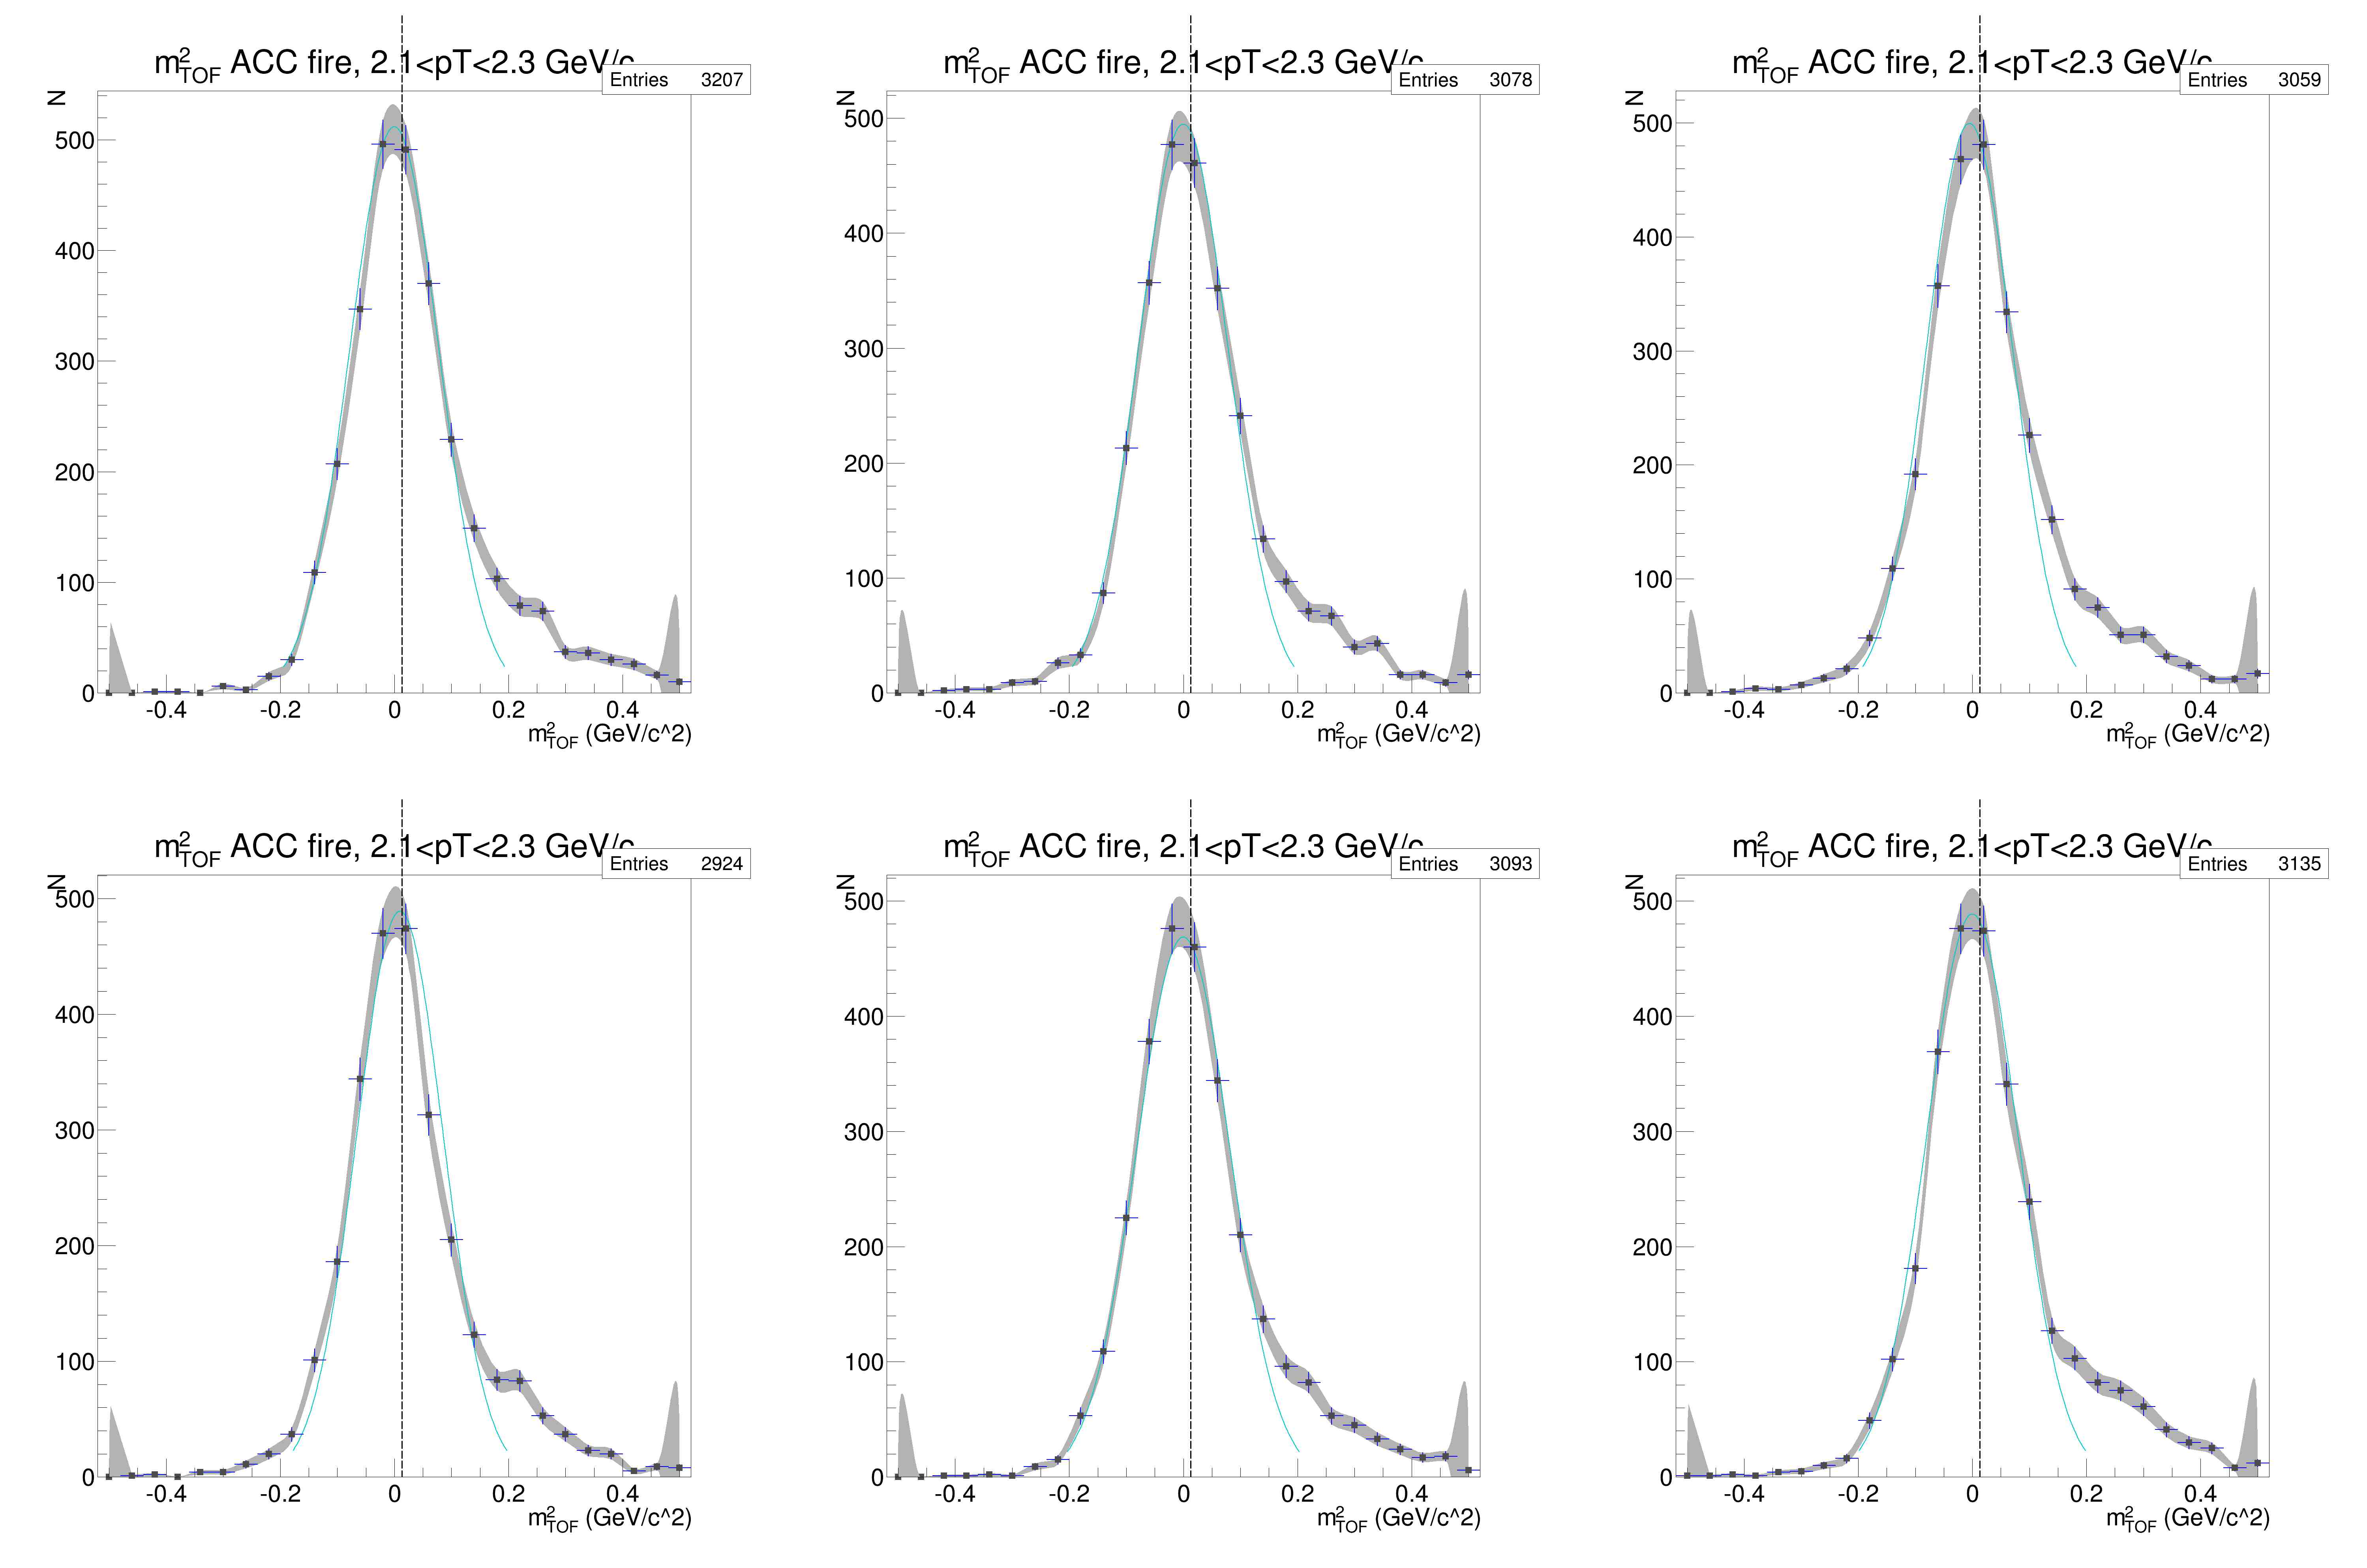
\includegraphics[width=1\textwidth]{hiptfits/neg/PSm2_cent0_ich0_accfire1_ptbin8.jpg}
    \caption{$m^2$ for ACC fired tracks}
    \end{subfigure}  
  \label{fig:acc21-23}
\end{figure}
\begin{figure}[H]
  \ContinuedFloat
    \begin{subfigure}{1\textwidth}
    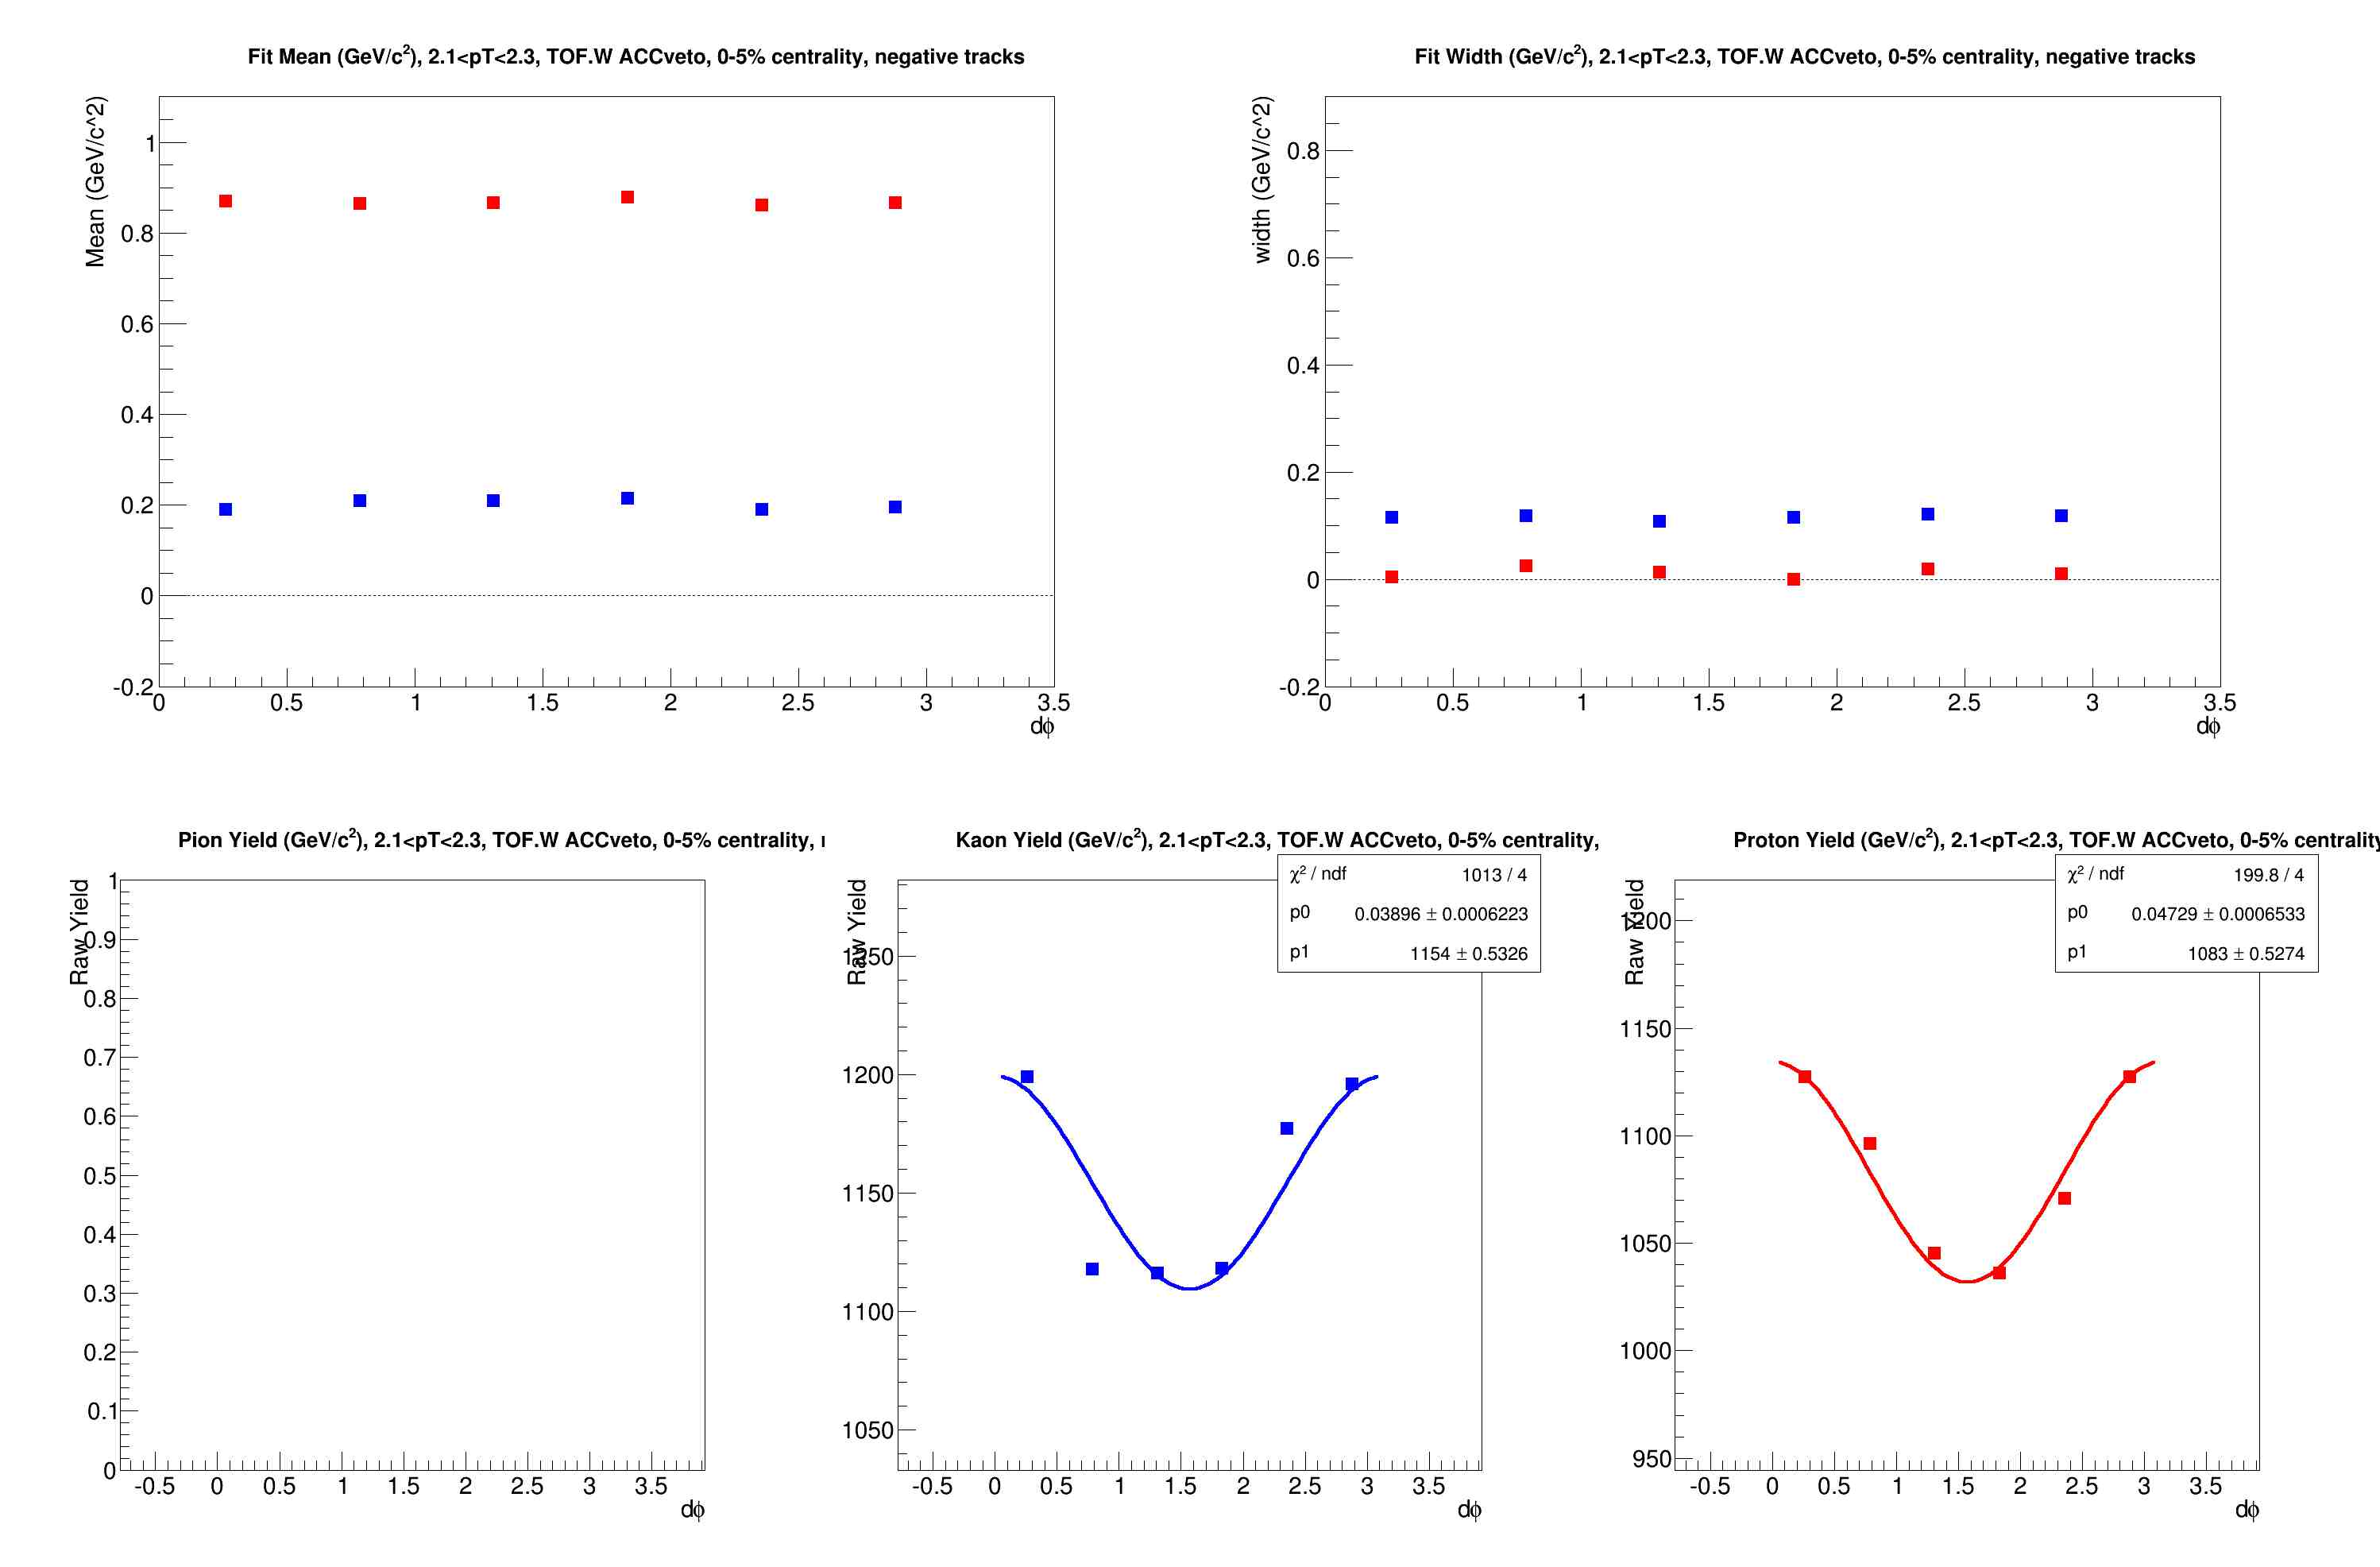
\includegraphics[width=1\textwidth]{hiptfits/neg/fitParams_tof2_cent0_ch0_pT-21-23.jpg}
    \caption{PID parameters and Yields for ACC vetoed tracks}
    \end{subfigure}    
    \begin{subfigure}{1\textwidth}
    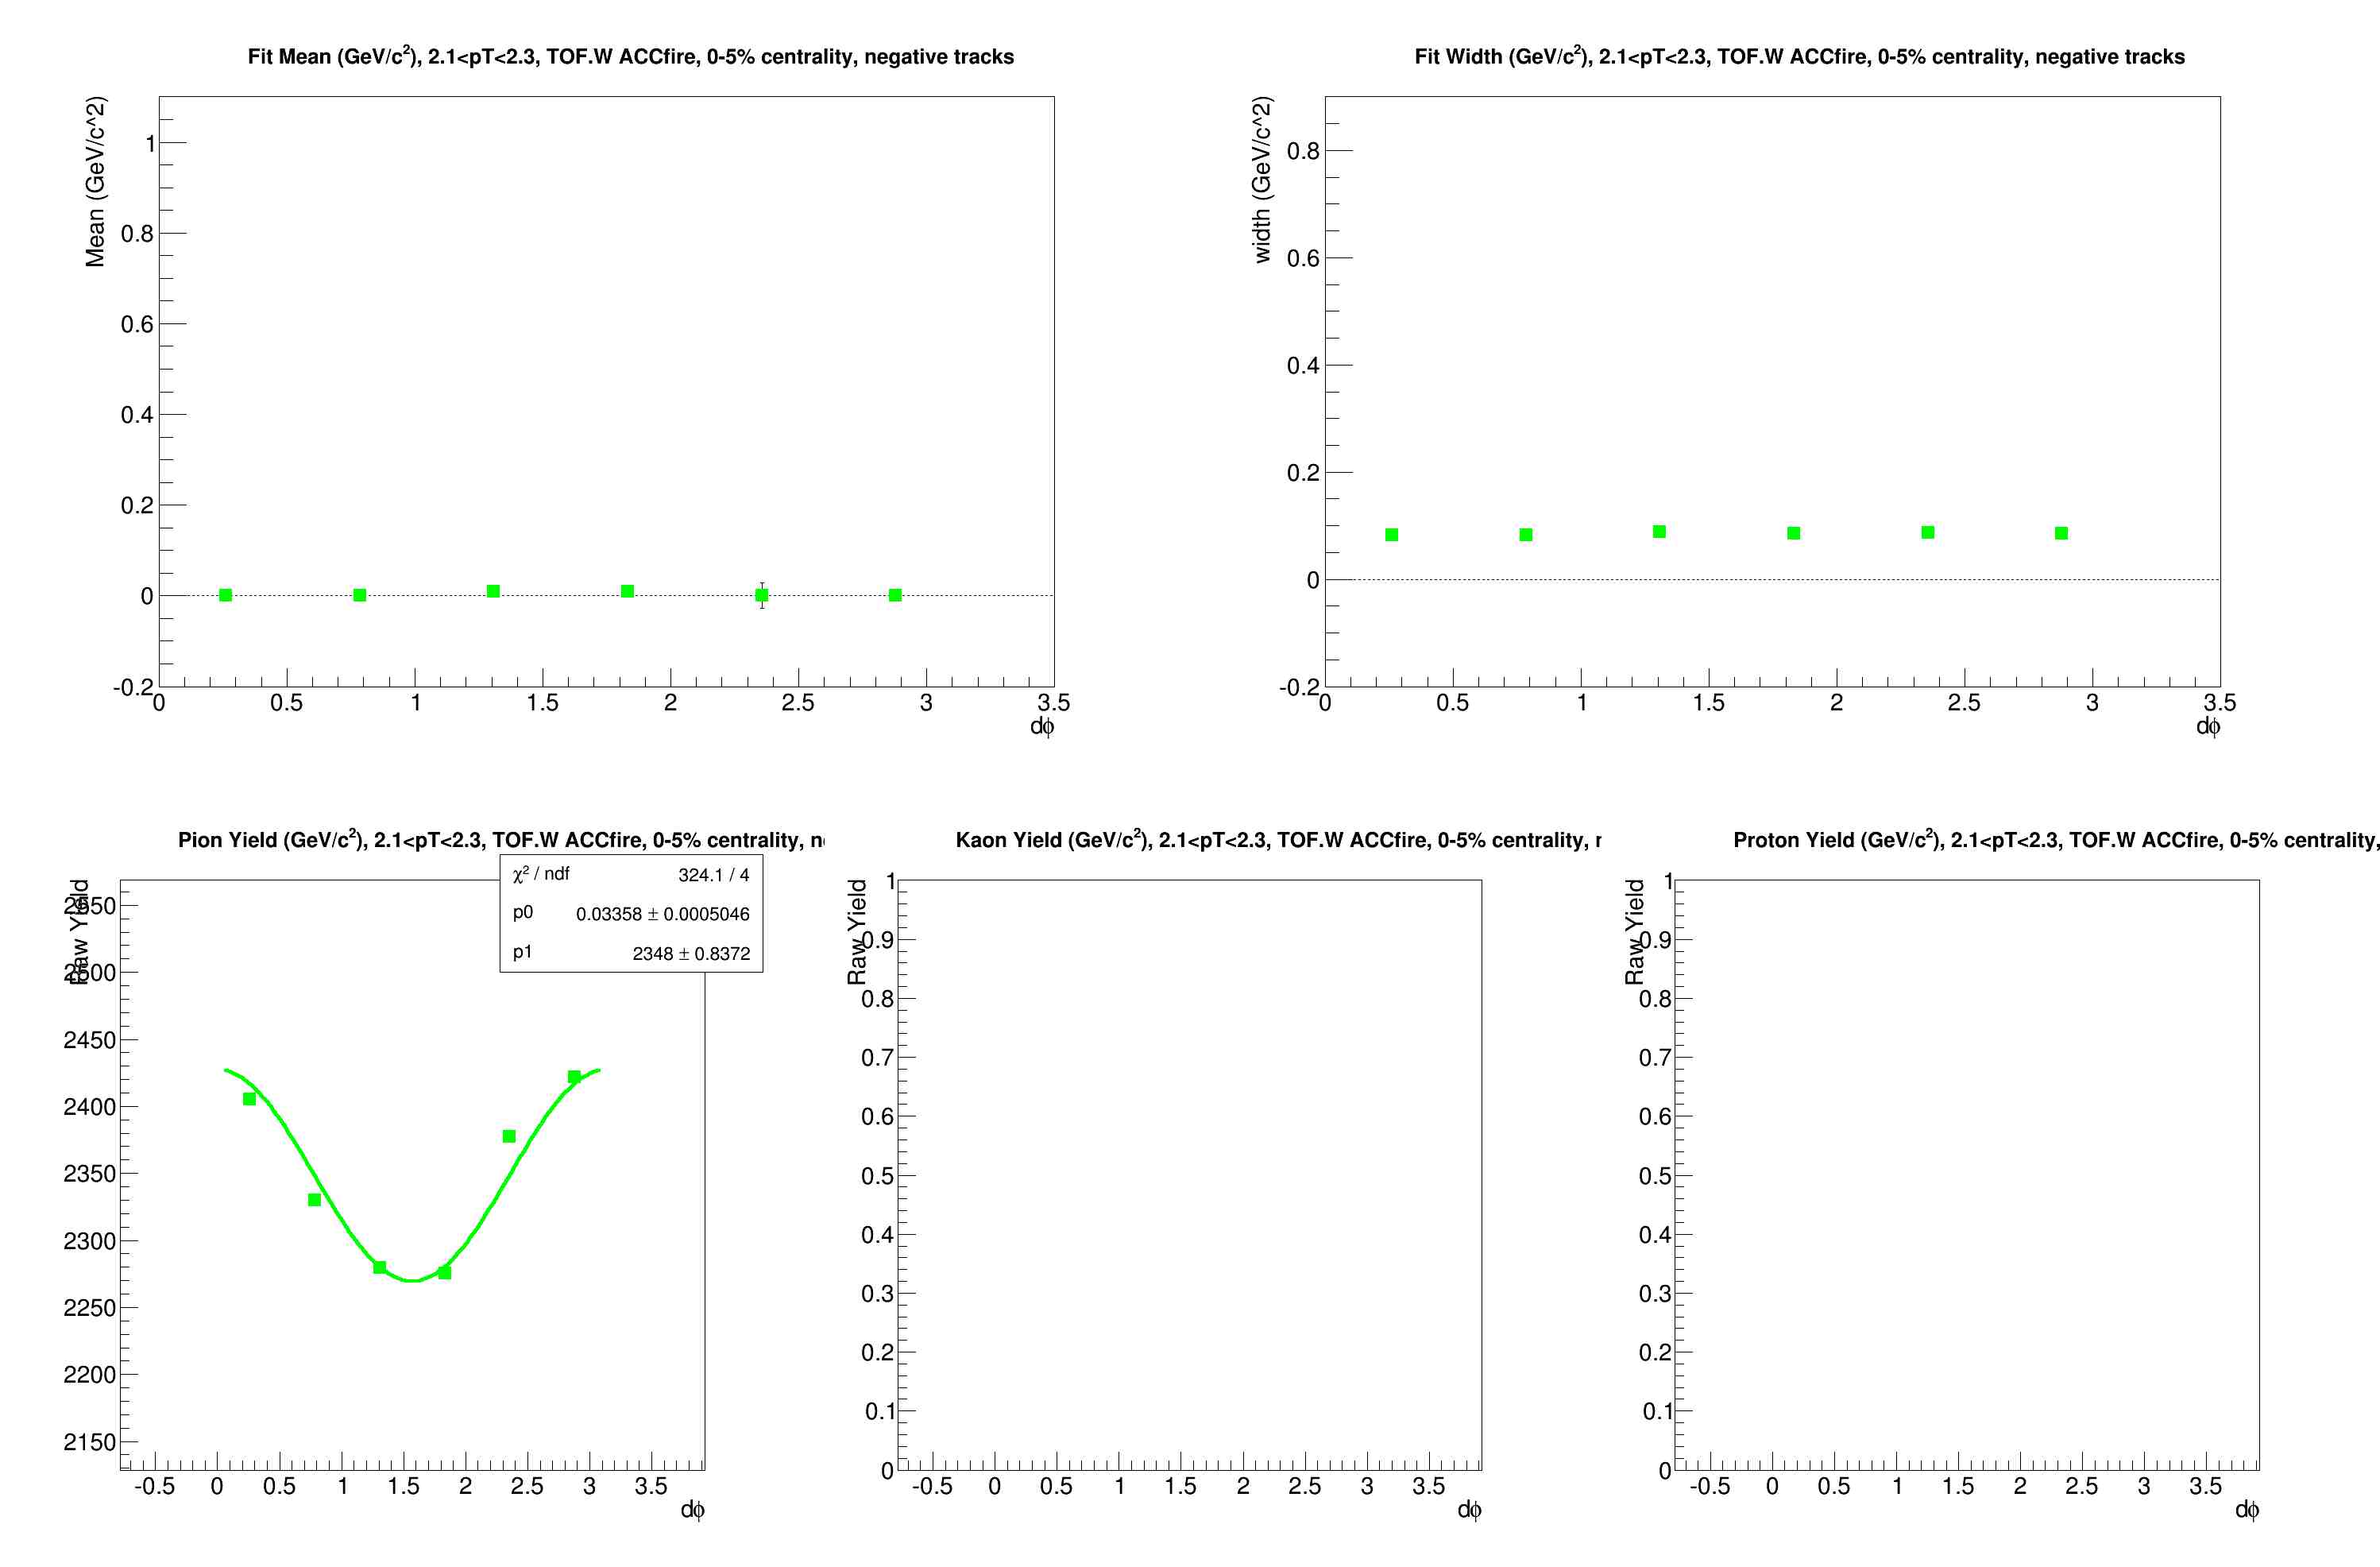
\includegraphics[width=1\textwidth]{hiptfits/neg/fitParams_tof3_cent0_ch0_pT-21-23.jpg}
    \caption{PID parameters and Yields for ACC fired tracks}
    \end{subfigure} 
    \rule{35em}{0.5pt}
  \caption[ACC $N_{p.e.}$ vs $m_2$, PID fits, and Yield vs $d\phi$ for $p_T$=2.1-2.3 GeV/c, TOF.W, negative particles]{ACC $N_{p.e.}$ vs $m_2$, PID fits, and Yield vs $d\phi$ for $p_T$=2.1-2.3 GeV/c, TOF.W, negative particles}
  \label{fig:acc21-23neg}
\end{figure}


\begin{figure}[H]
  \centering
    \begin{subfigure}{1\textwidth}
    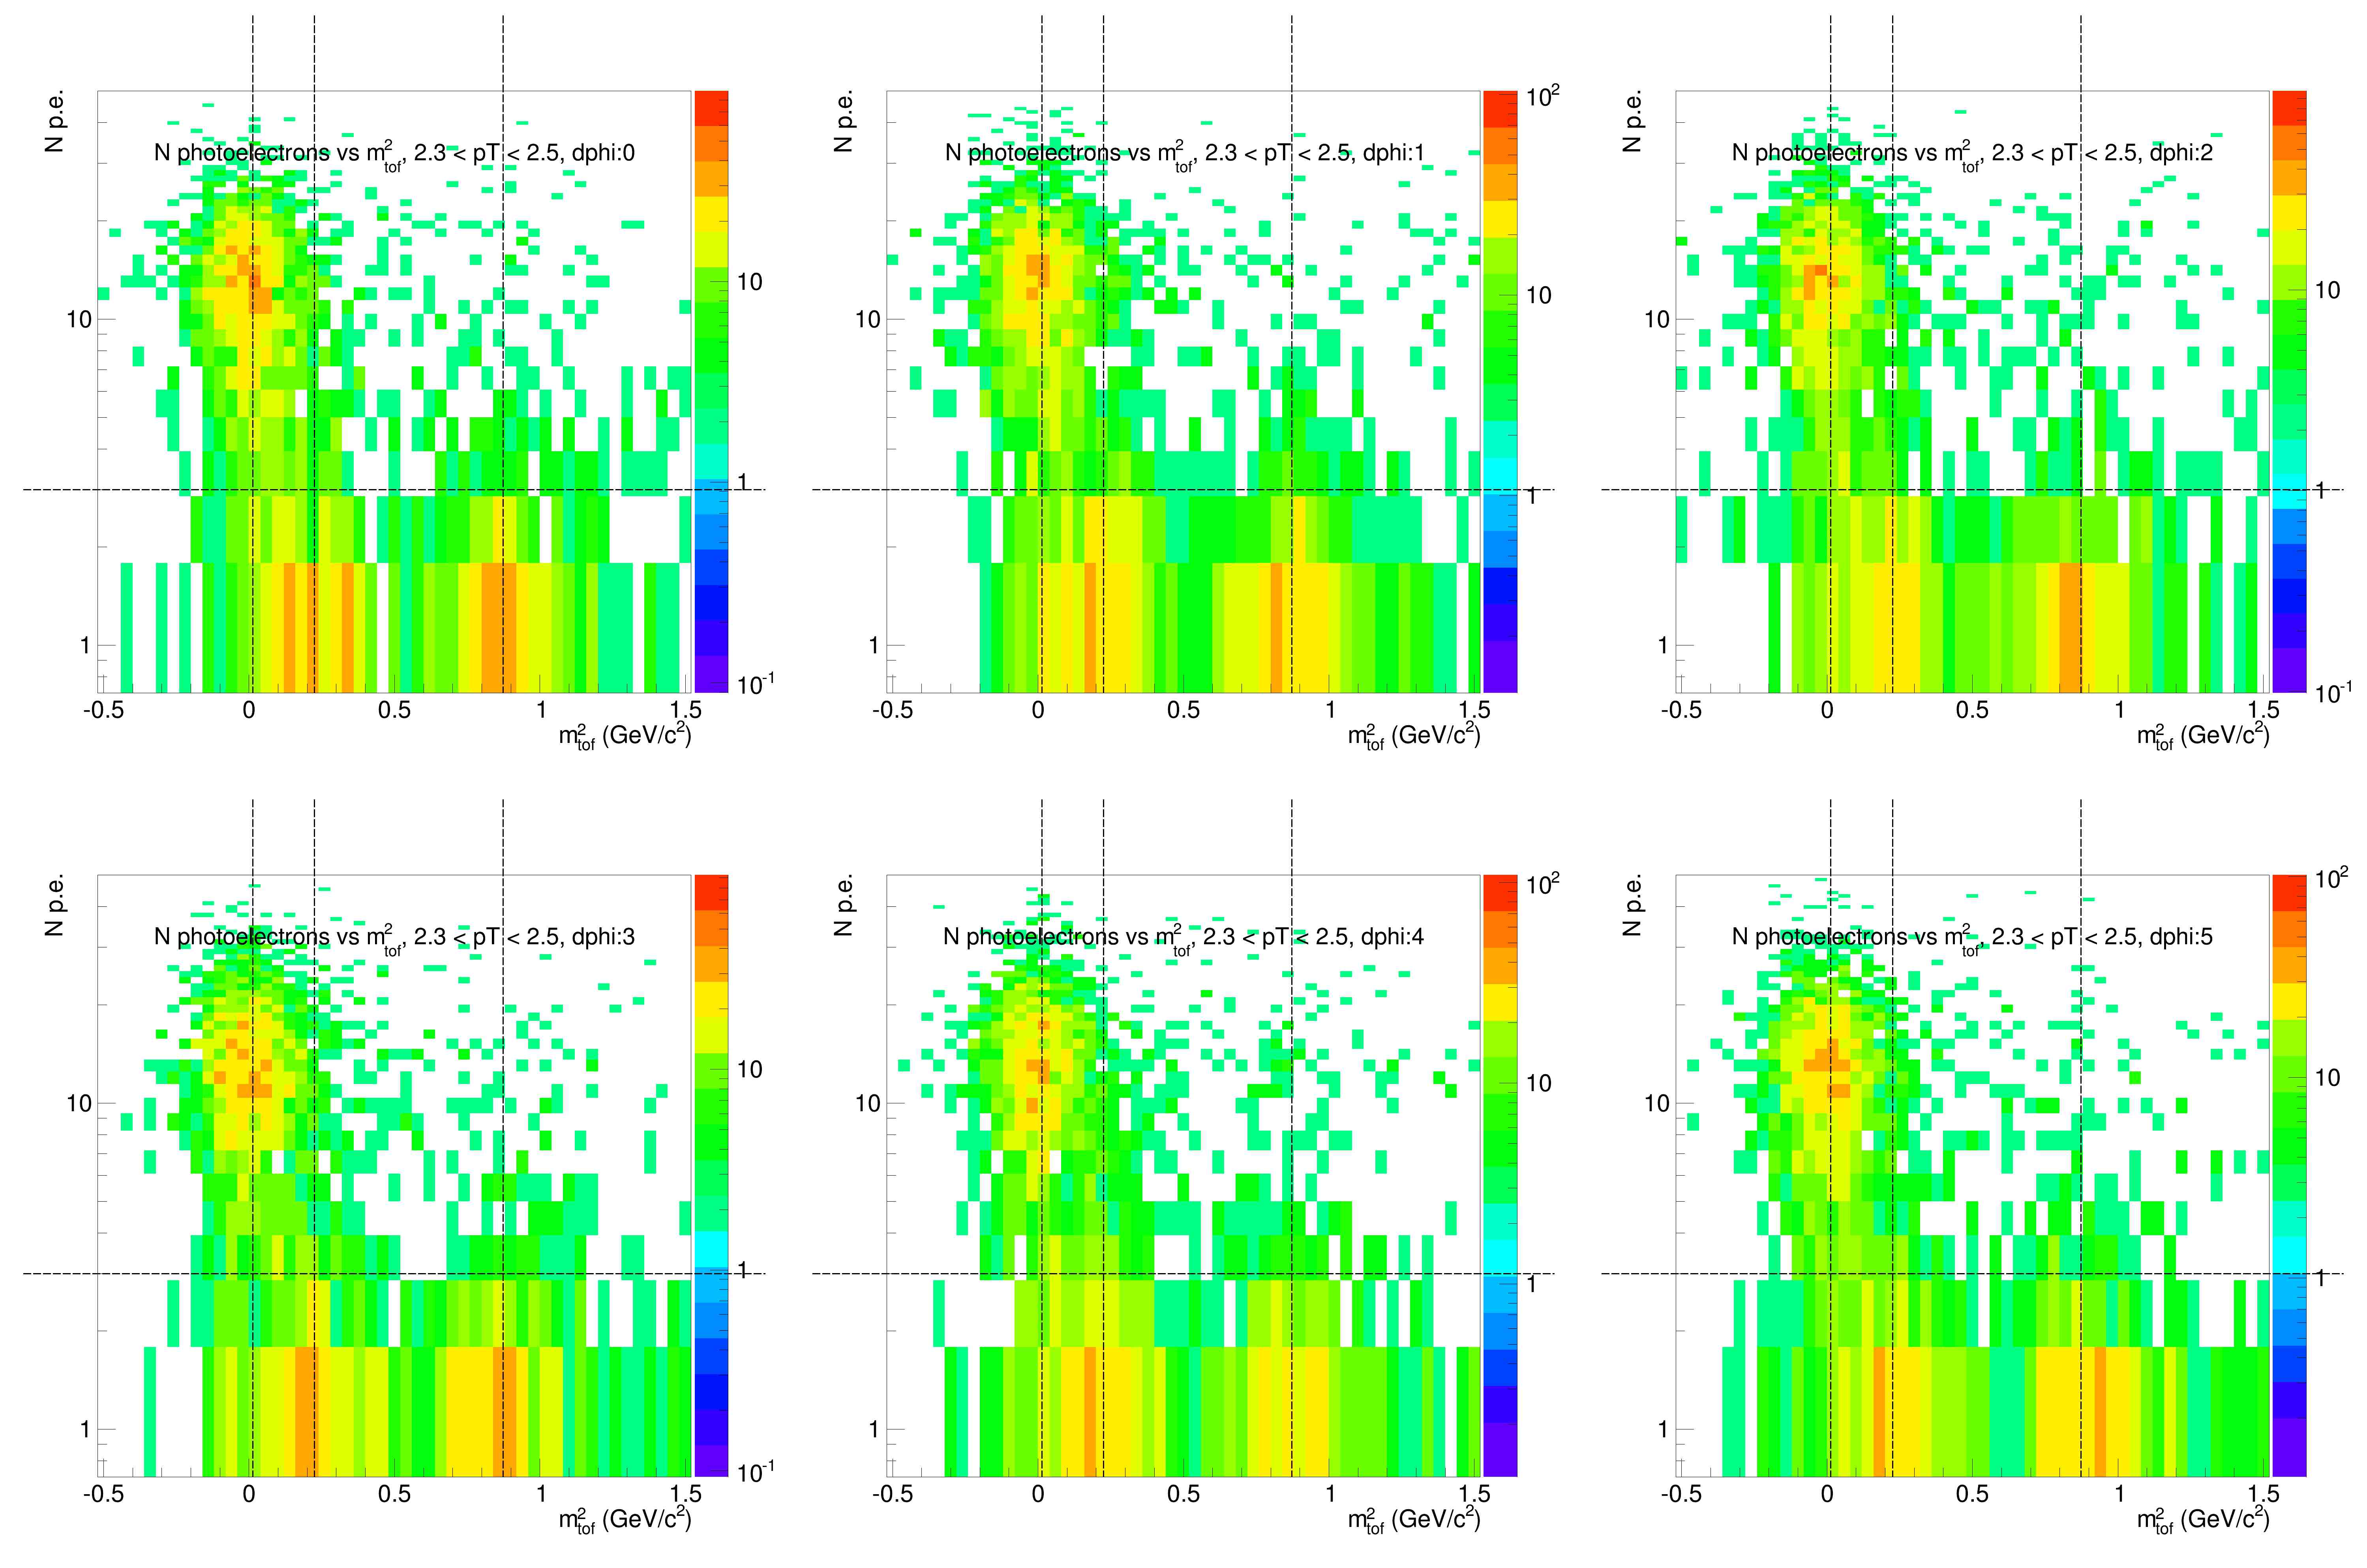
\includegraphics[width=1\textwidth]{hiptfits/neg/PSaccthreshold_cent0_ich0_accfire0_ptbin9.jpg}
    \caption{$N_{p.e.}$ vs $m^2$}
    \end{subfigure}
\end{figure}
\begin{figure}[H]
  \ContinuedFloat
    \begin{subfigure}{1\textwidth}
    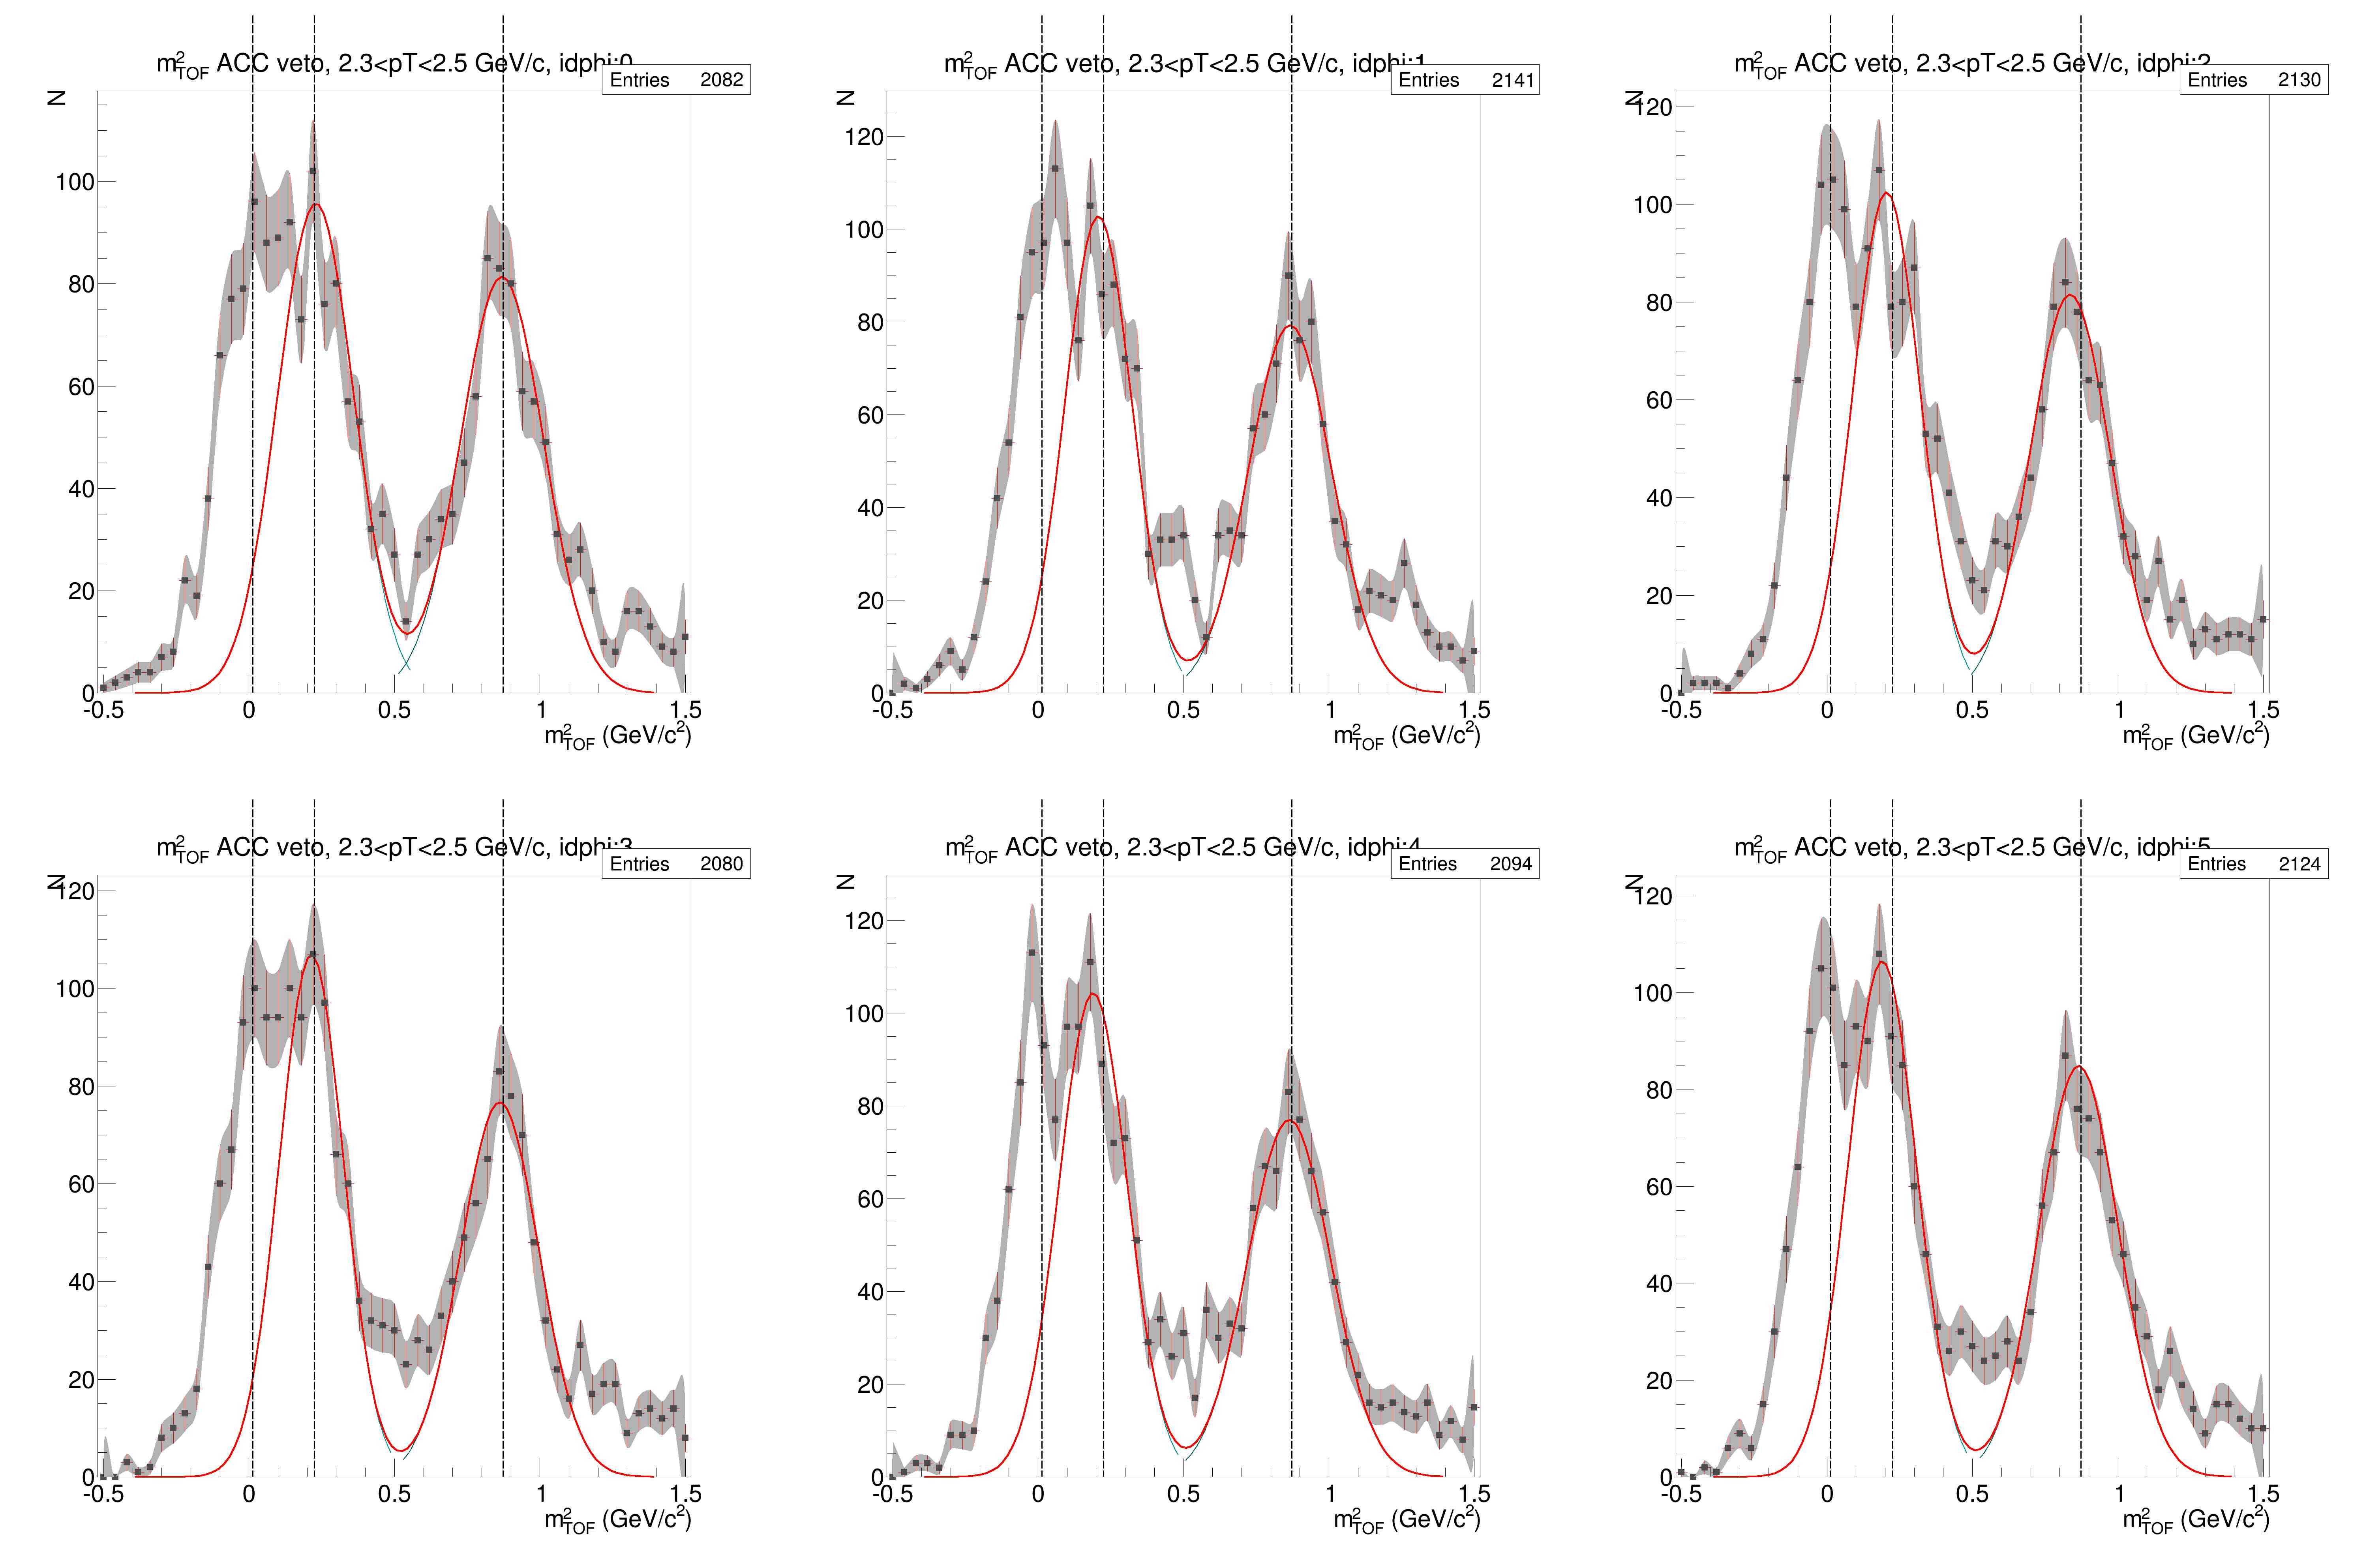
\includegraphics[width=1\textwidth]{hiptfits/neg/PSm2_cent0_ich0_accfire0_ptbin9.jpg}
    \caption{$m^2$ for ACC vetoed tracks}
    \end{subfigure}
    \begin{subfigure}{1\textwidth}
    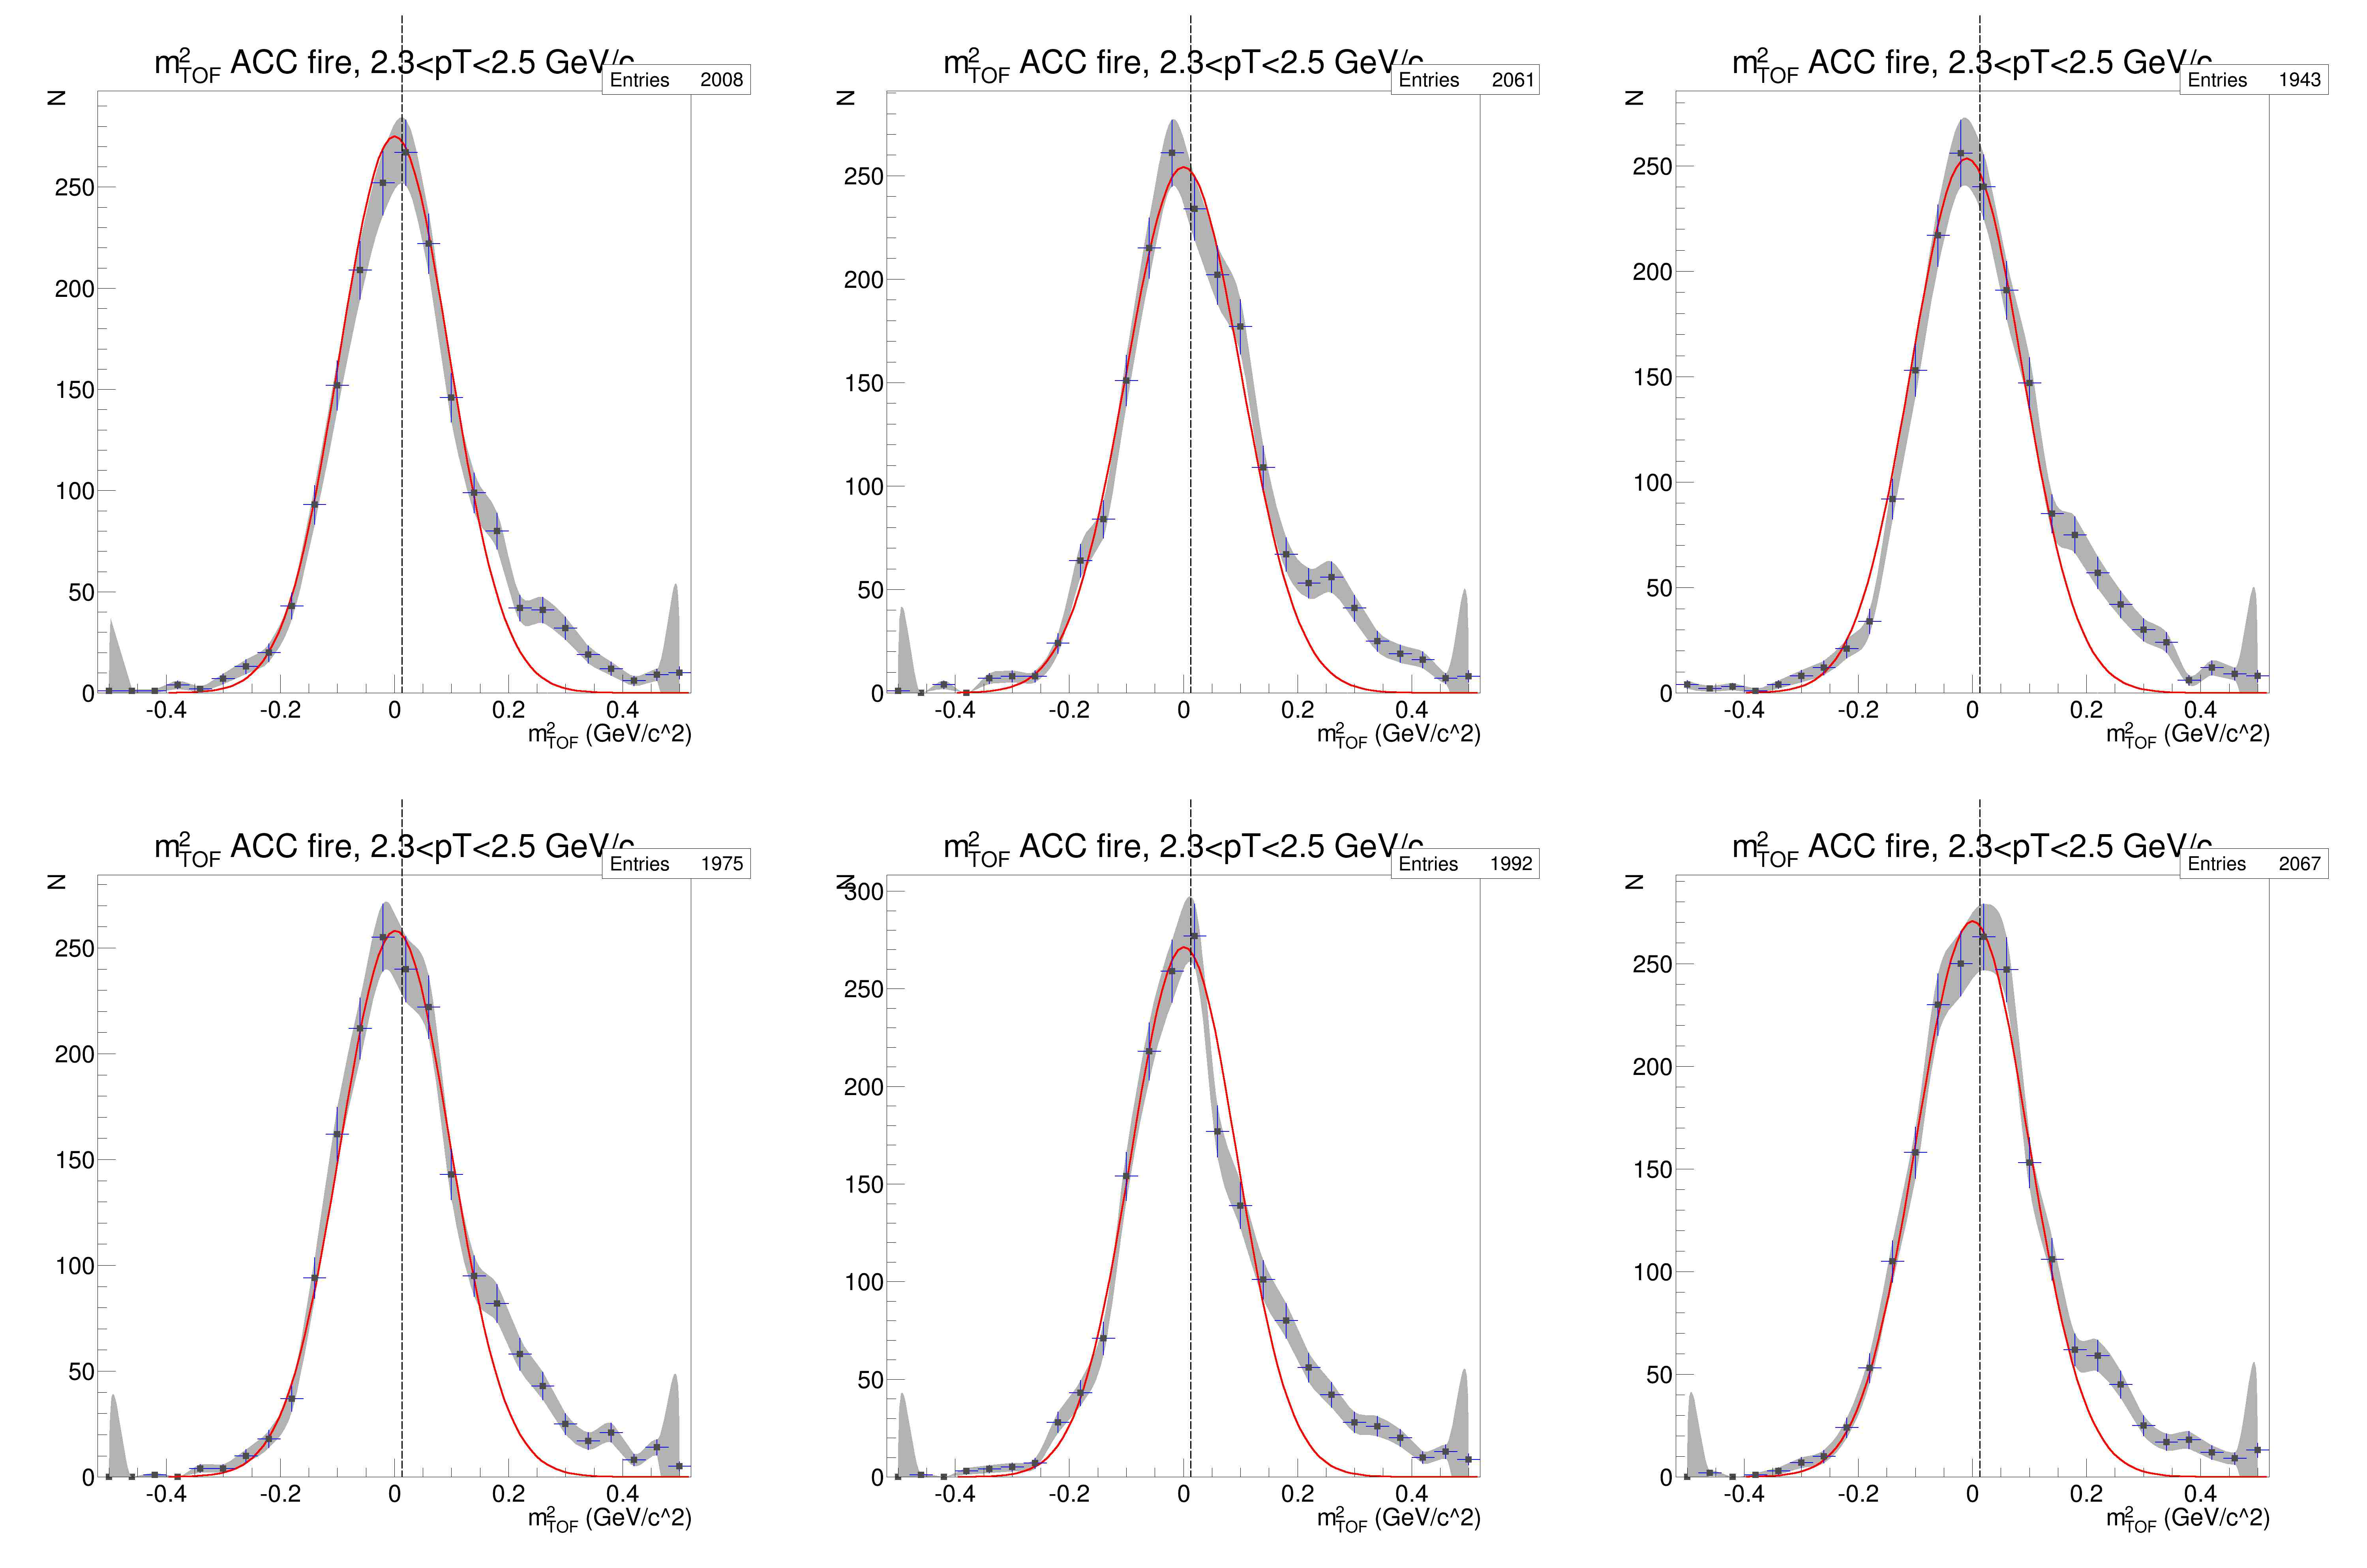
\includegraphics[width=1\textwidth]{hiptfits/neg/PSm2_cent0_ich0_accfire1_ptbin9.jpg}
    \caption{$m^2$ for ACC fired tracks}
    \end{subfigure}  
\end{figure}
\begin{figure}[H]
  \ContinuedFloat
    \begin{subfigure}{1\textwidth}
    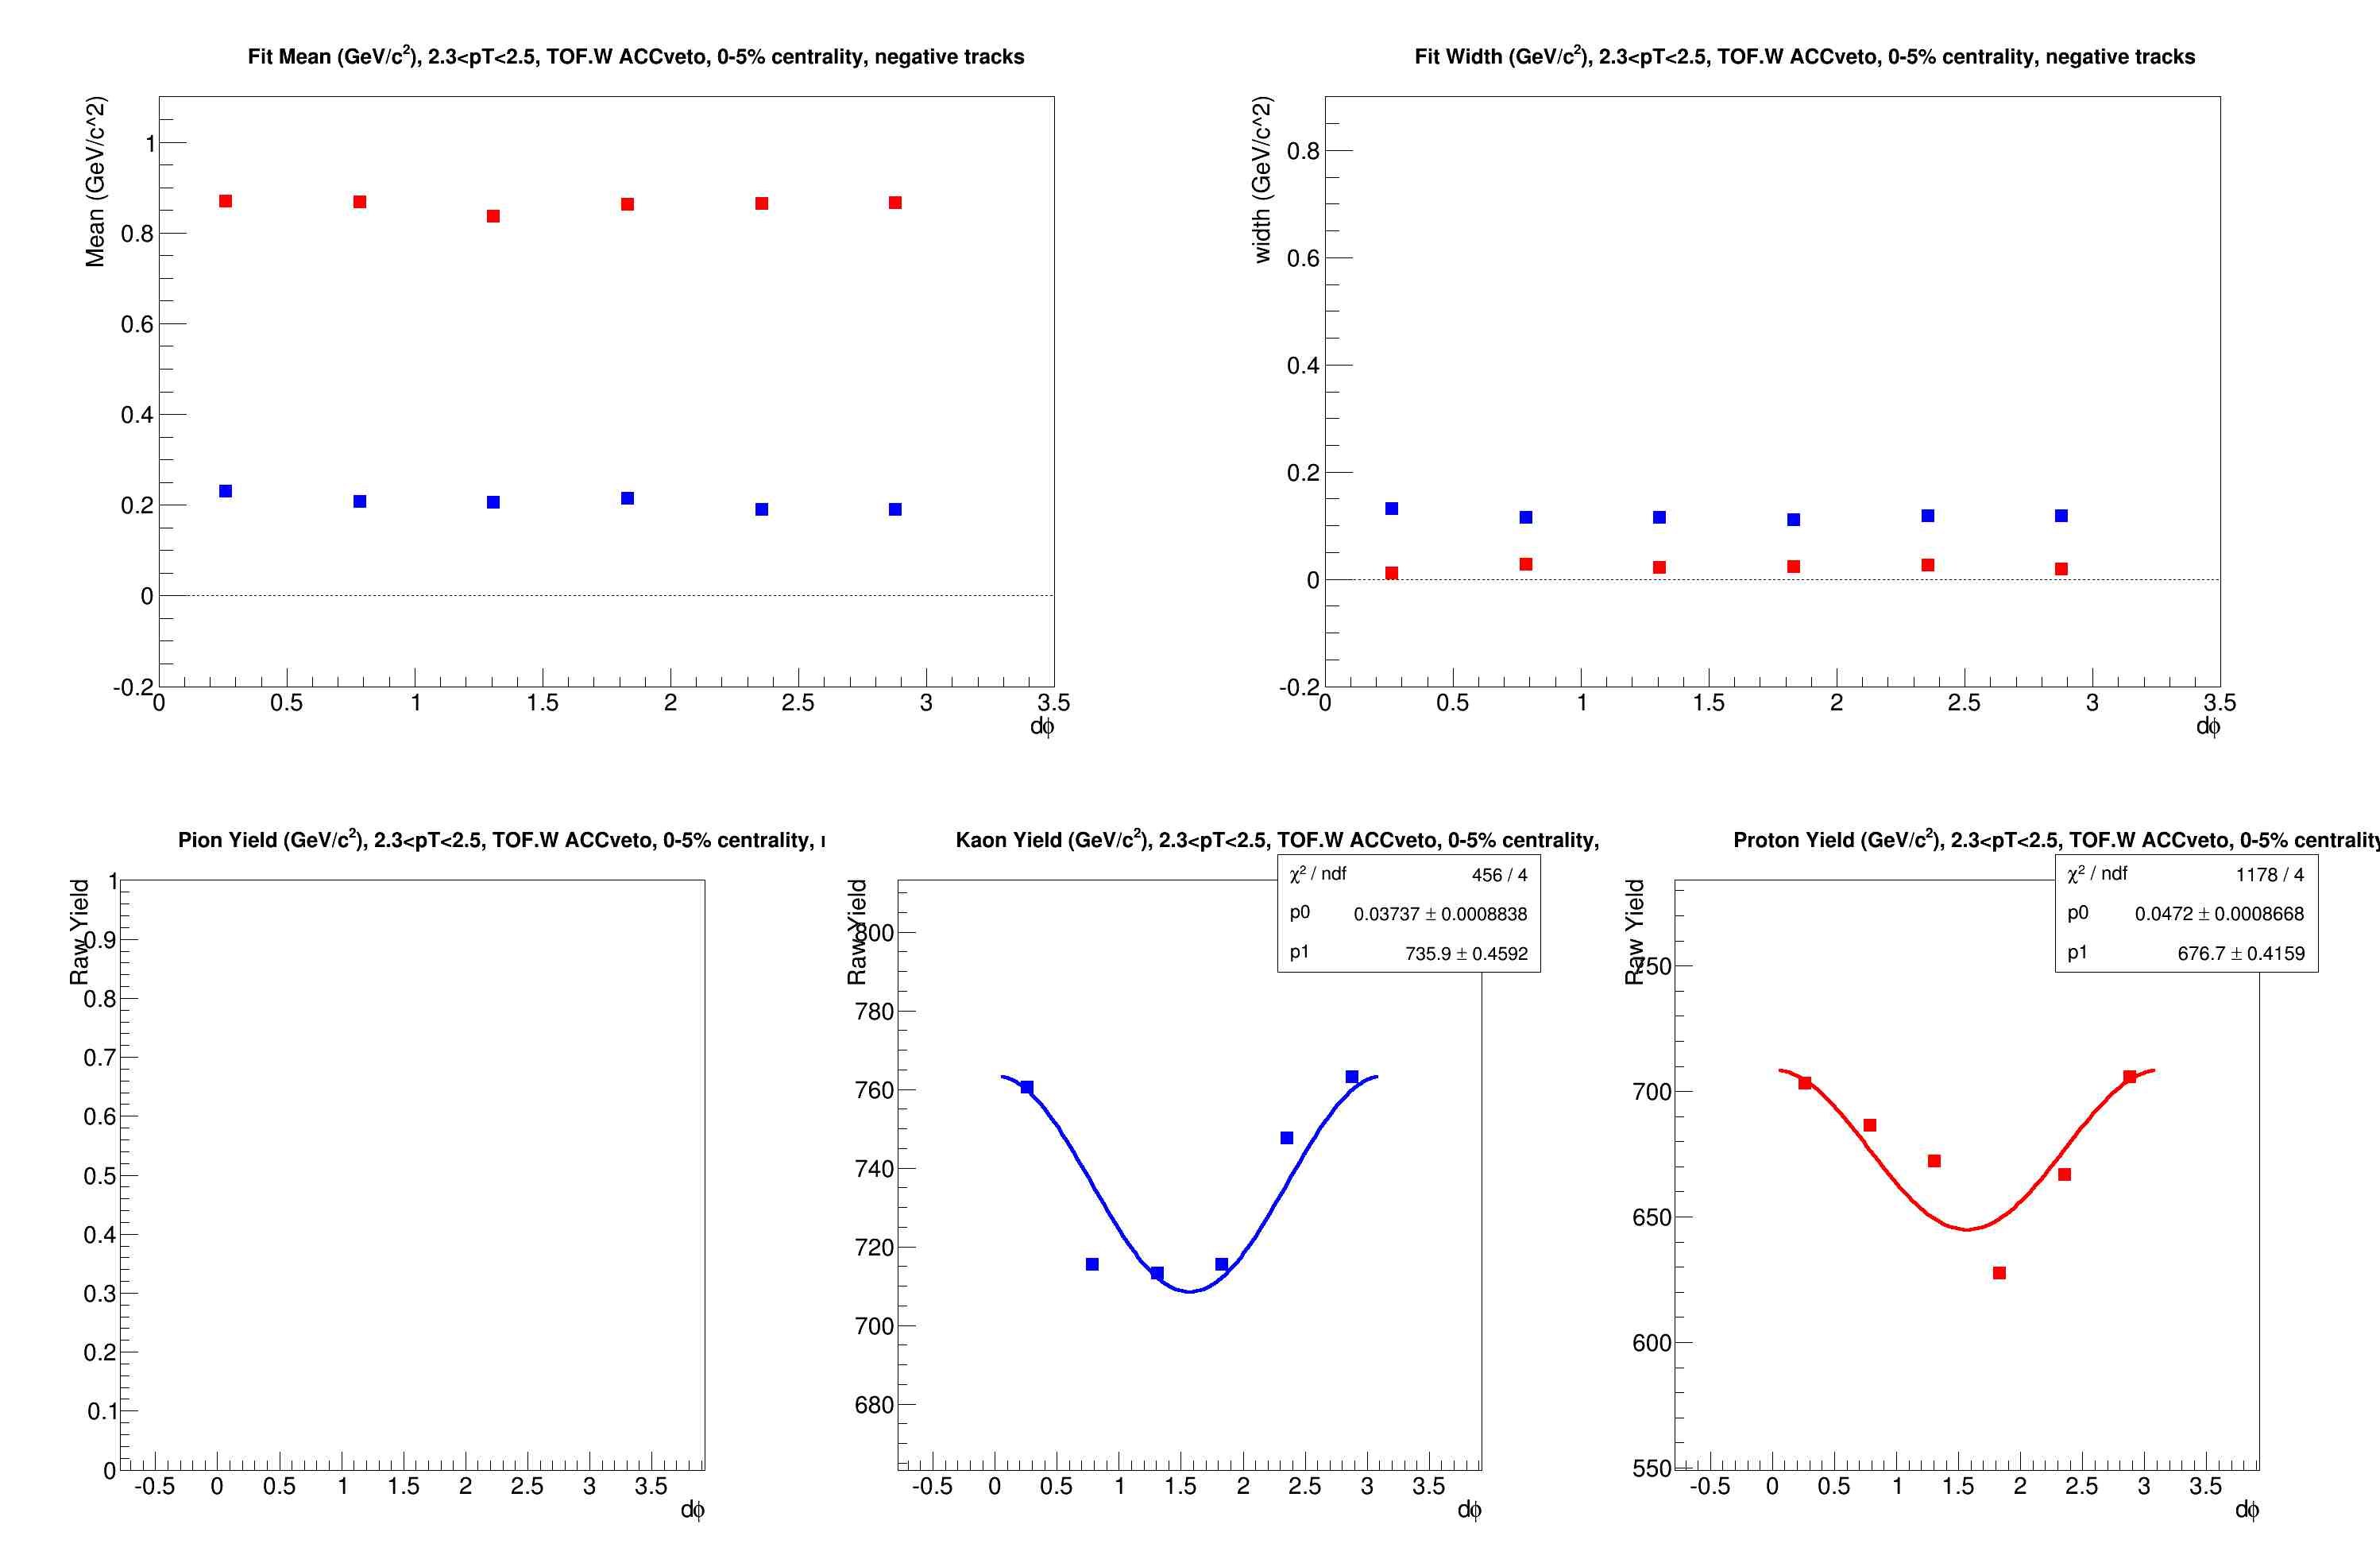
\includegraphics[width=1\textwidth]{hiptfits/neg/fitParams_tof2_cent0_ch0_pT-23-25.jpg}
    \caption{PID parameters and Yields for ACC vetoed tracks}
    \end{subfigure}    
    \begin{subfigure}{1\textwidth}
    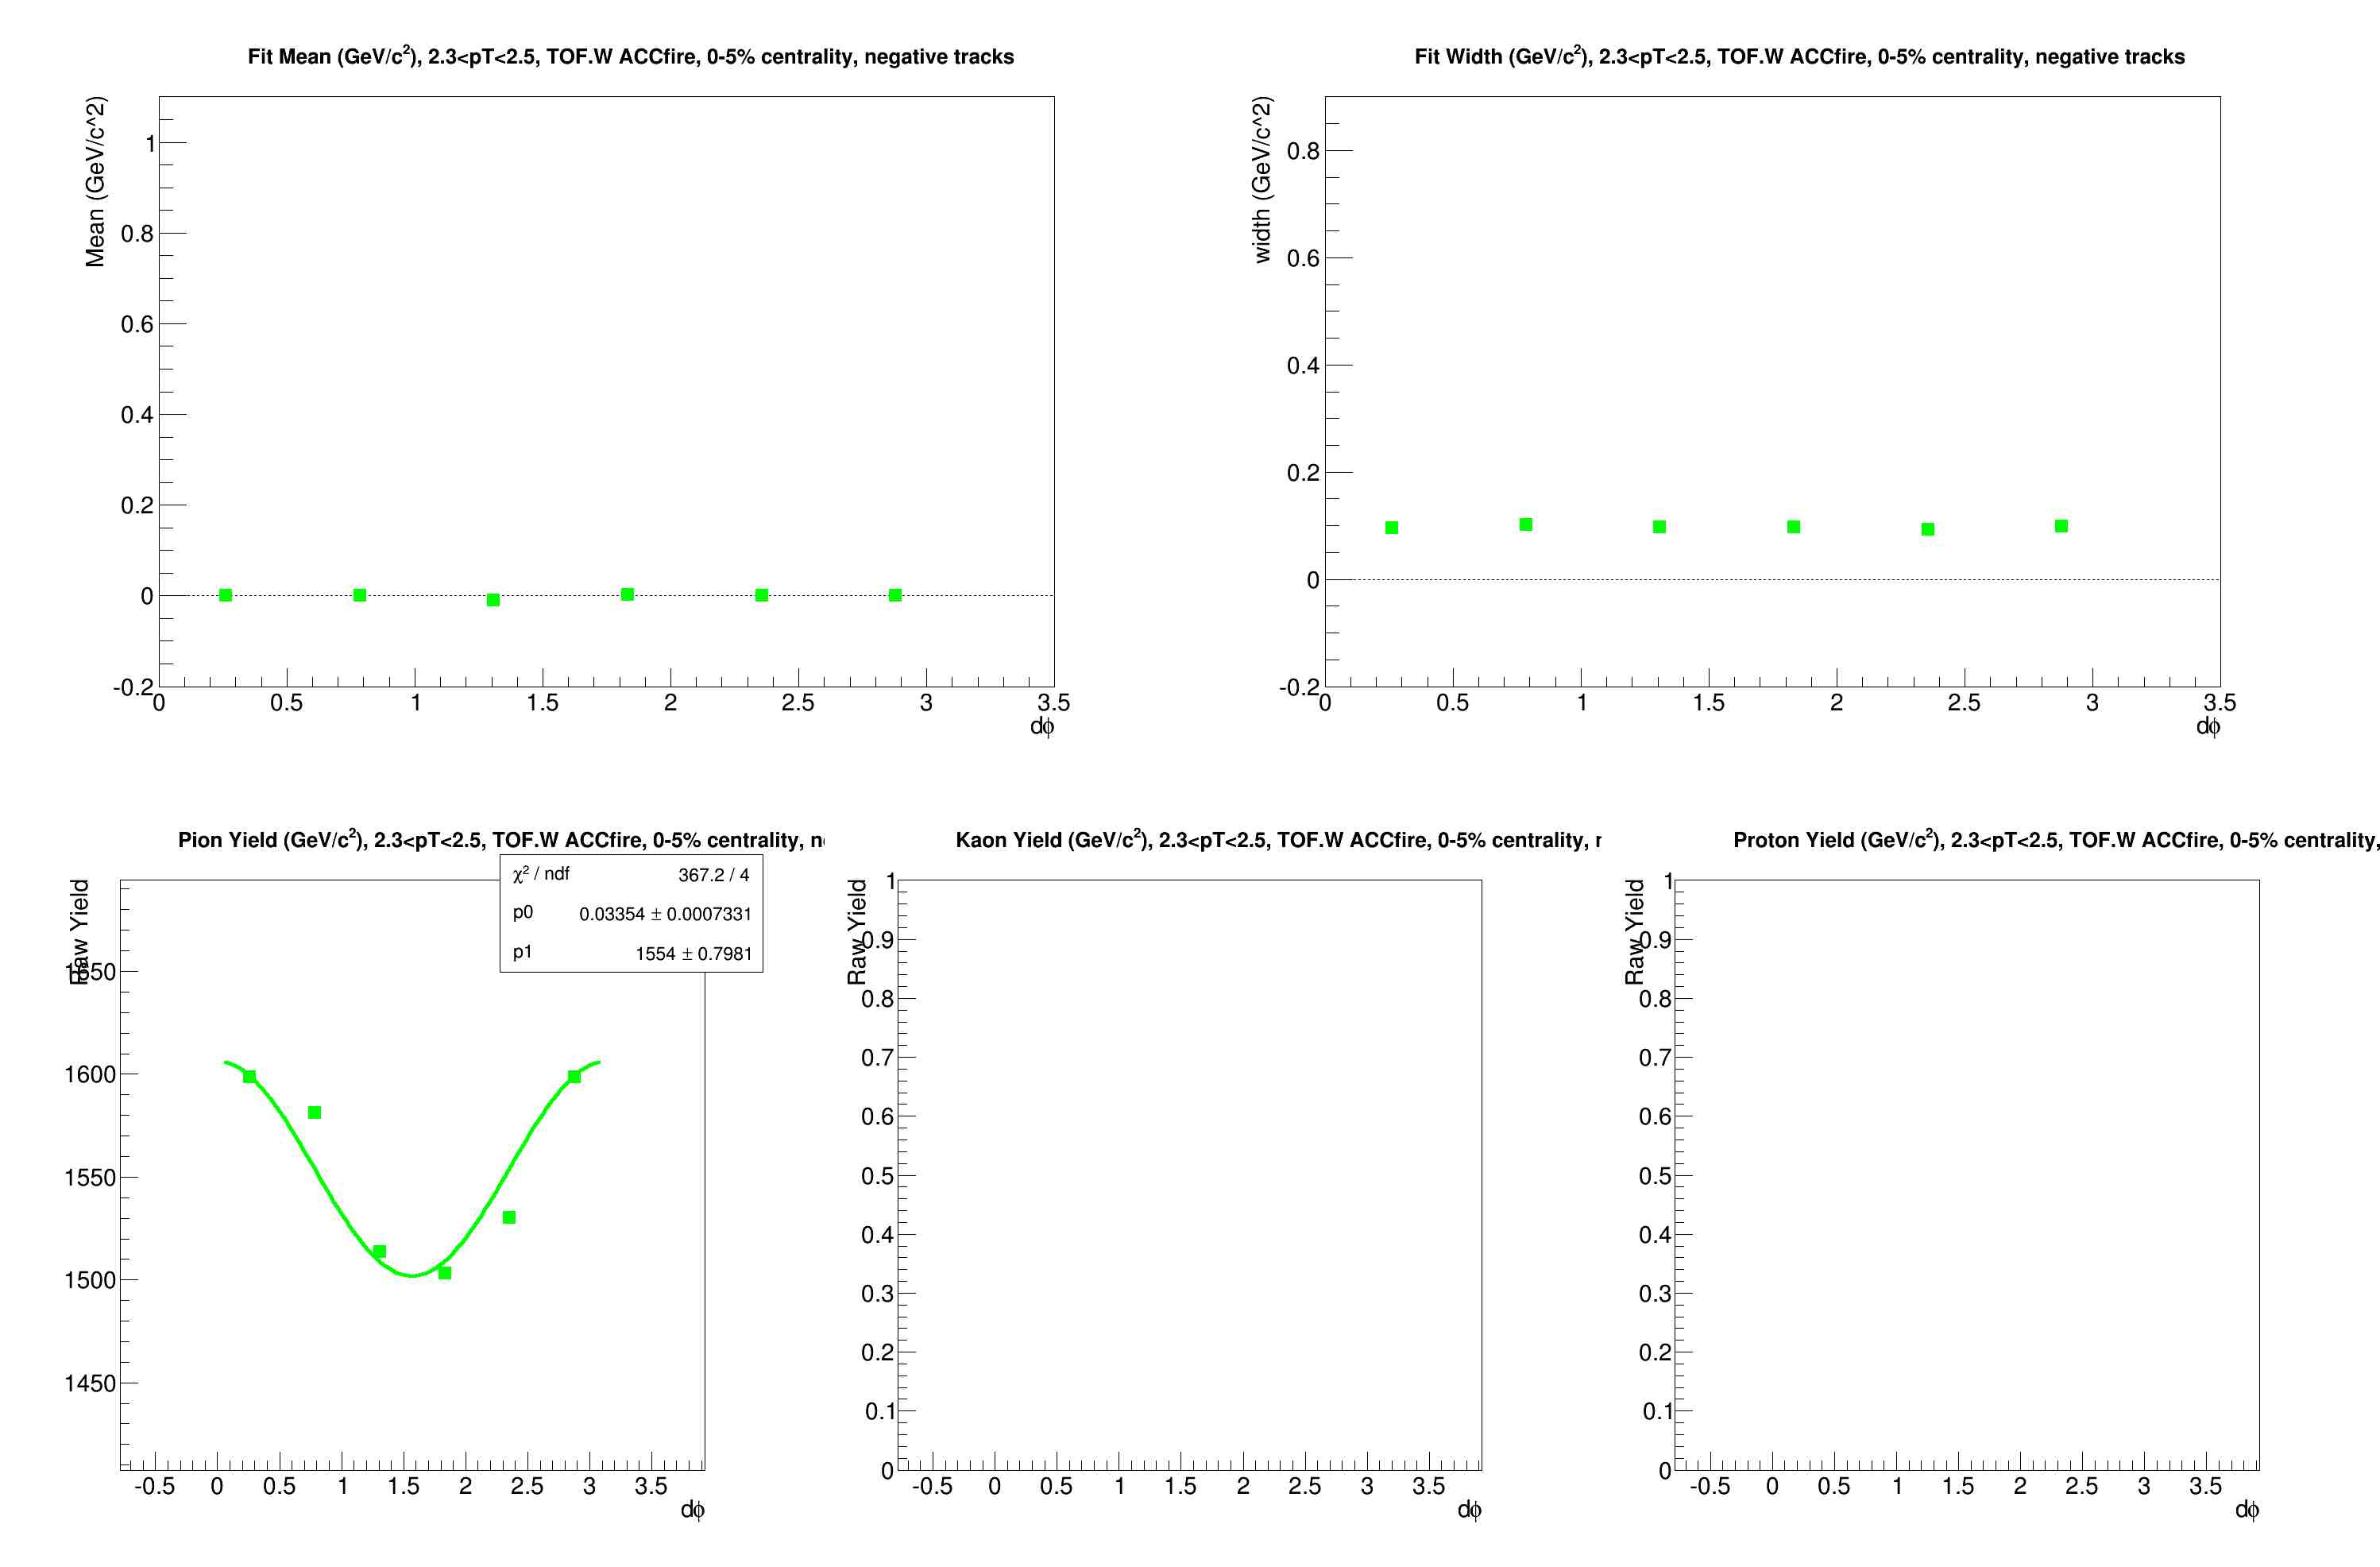
\includegraphics[width=1\textwidth]{hiptfits/neg/fitParams_tof3_cent0_ch0_pT-23-25.jpg}
    \caption{PID parameters and Yields for ACC fired tracks}
    \end{subfigure} 
    \rule{35em}{0.5pt}
  \caption[ACC $N_{p.e.}$ vs $m_2$, PID fits, and Yield vs $d\phi$ for $p_T$=2.3-2.5 GeV/c, TOF.W, negative particles]{ACC $N_{p.e.}$ vs $m_2$, PID fits, and Yield vs $d\phi$ for $p_T$=2.3-2.5 GeV/c, TOF.W, negative particles}
  \label{fig:acc23-25neg}
\end{figure}


\begin{figure}[H]
  \centering
    \begin{subfigure}{1\textwidth}
    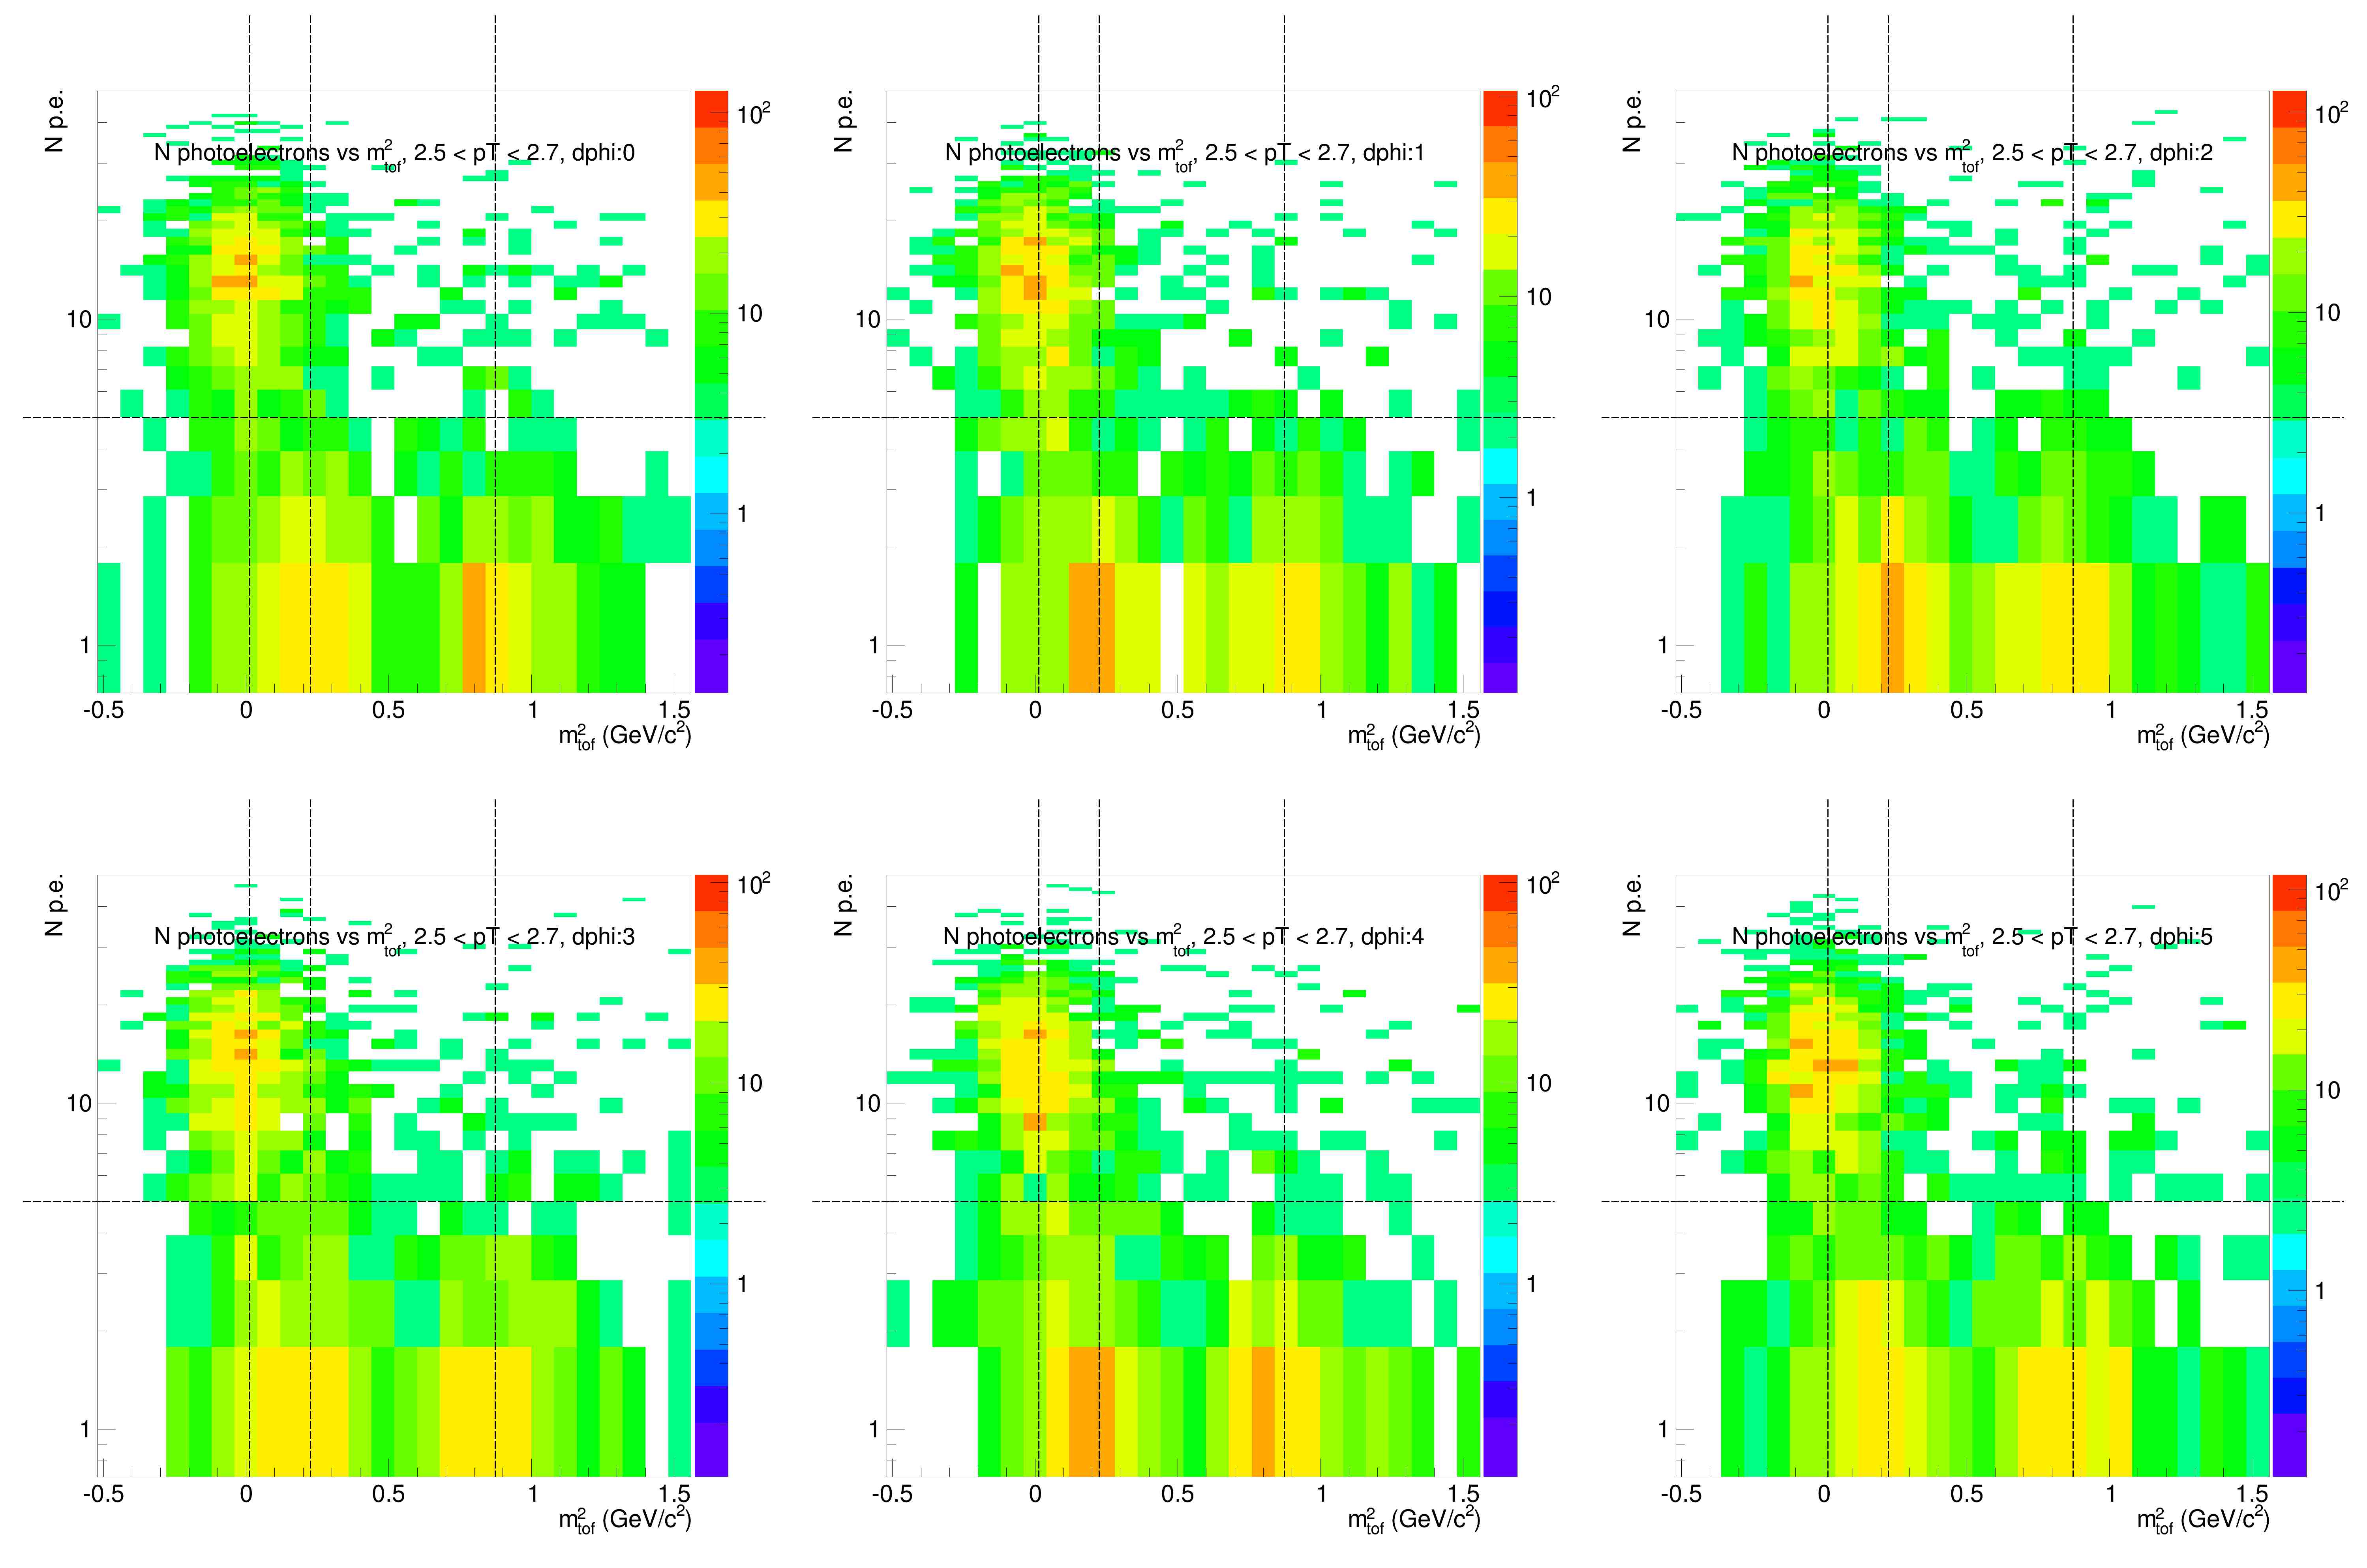
\includegraphics[width=1\textwidth]{hiptfits/neg/PSaccthreshold_cent0_ich0_accfire0_ptbin10.jpg}
    \caption{$N_{p.e.}$ vs $m^2$}
    \end{subfigure}
\end{figure}
\begin{figure}[H]
  \ContinuedFloat
    \begin{subfigure}{1\textwidth}
    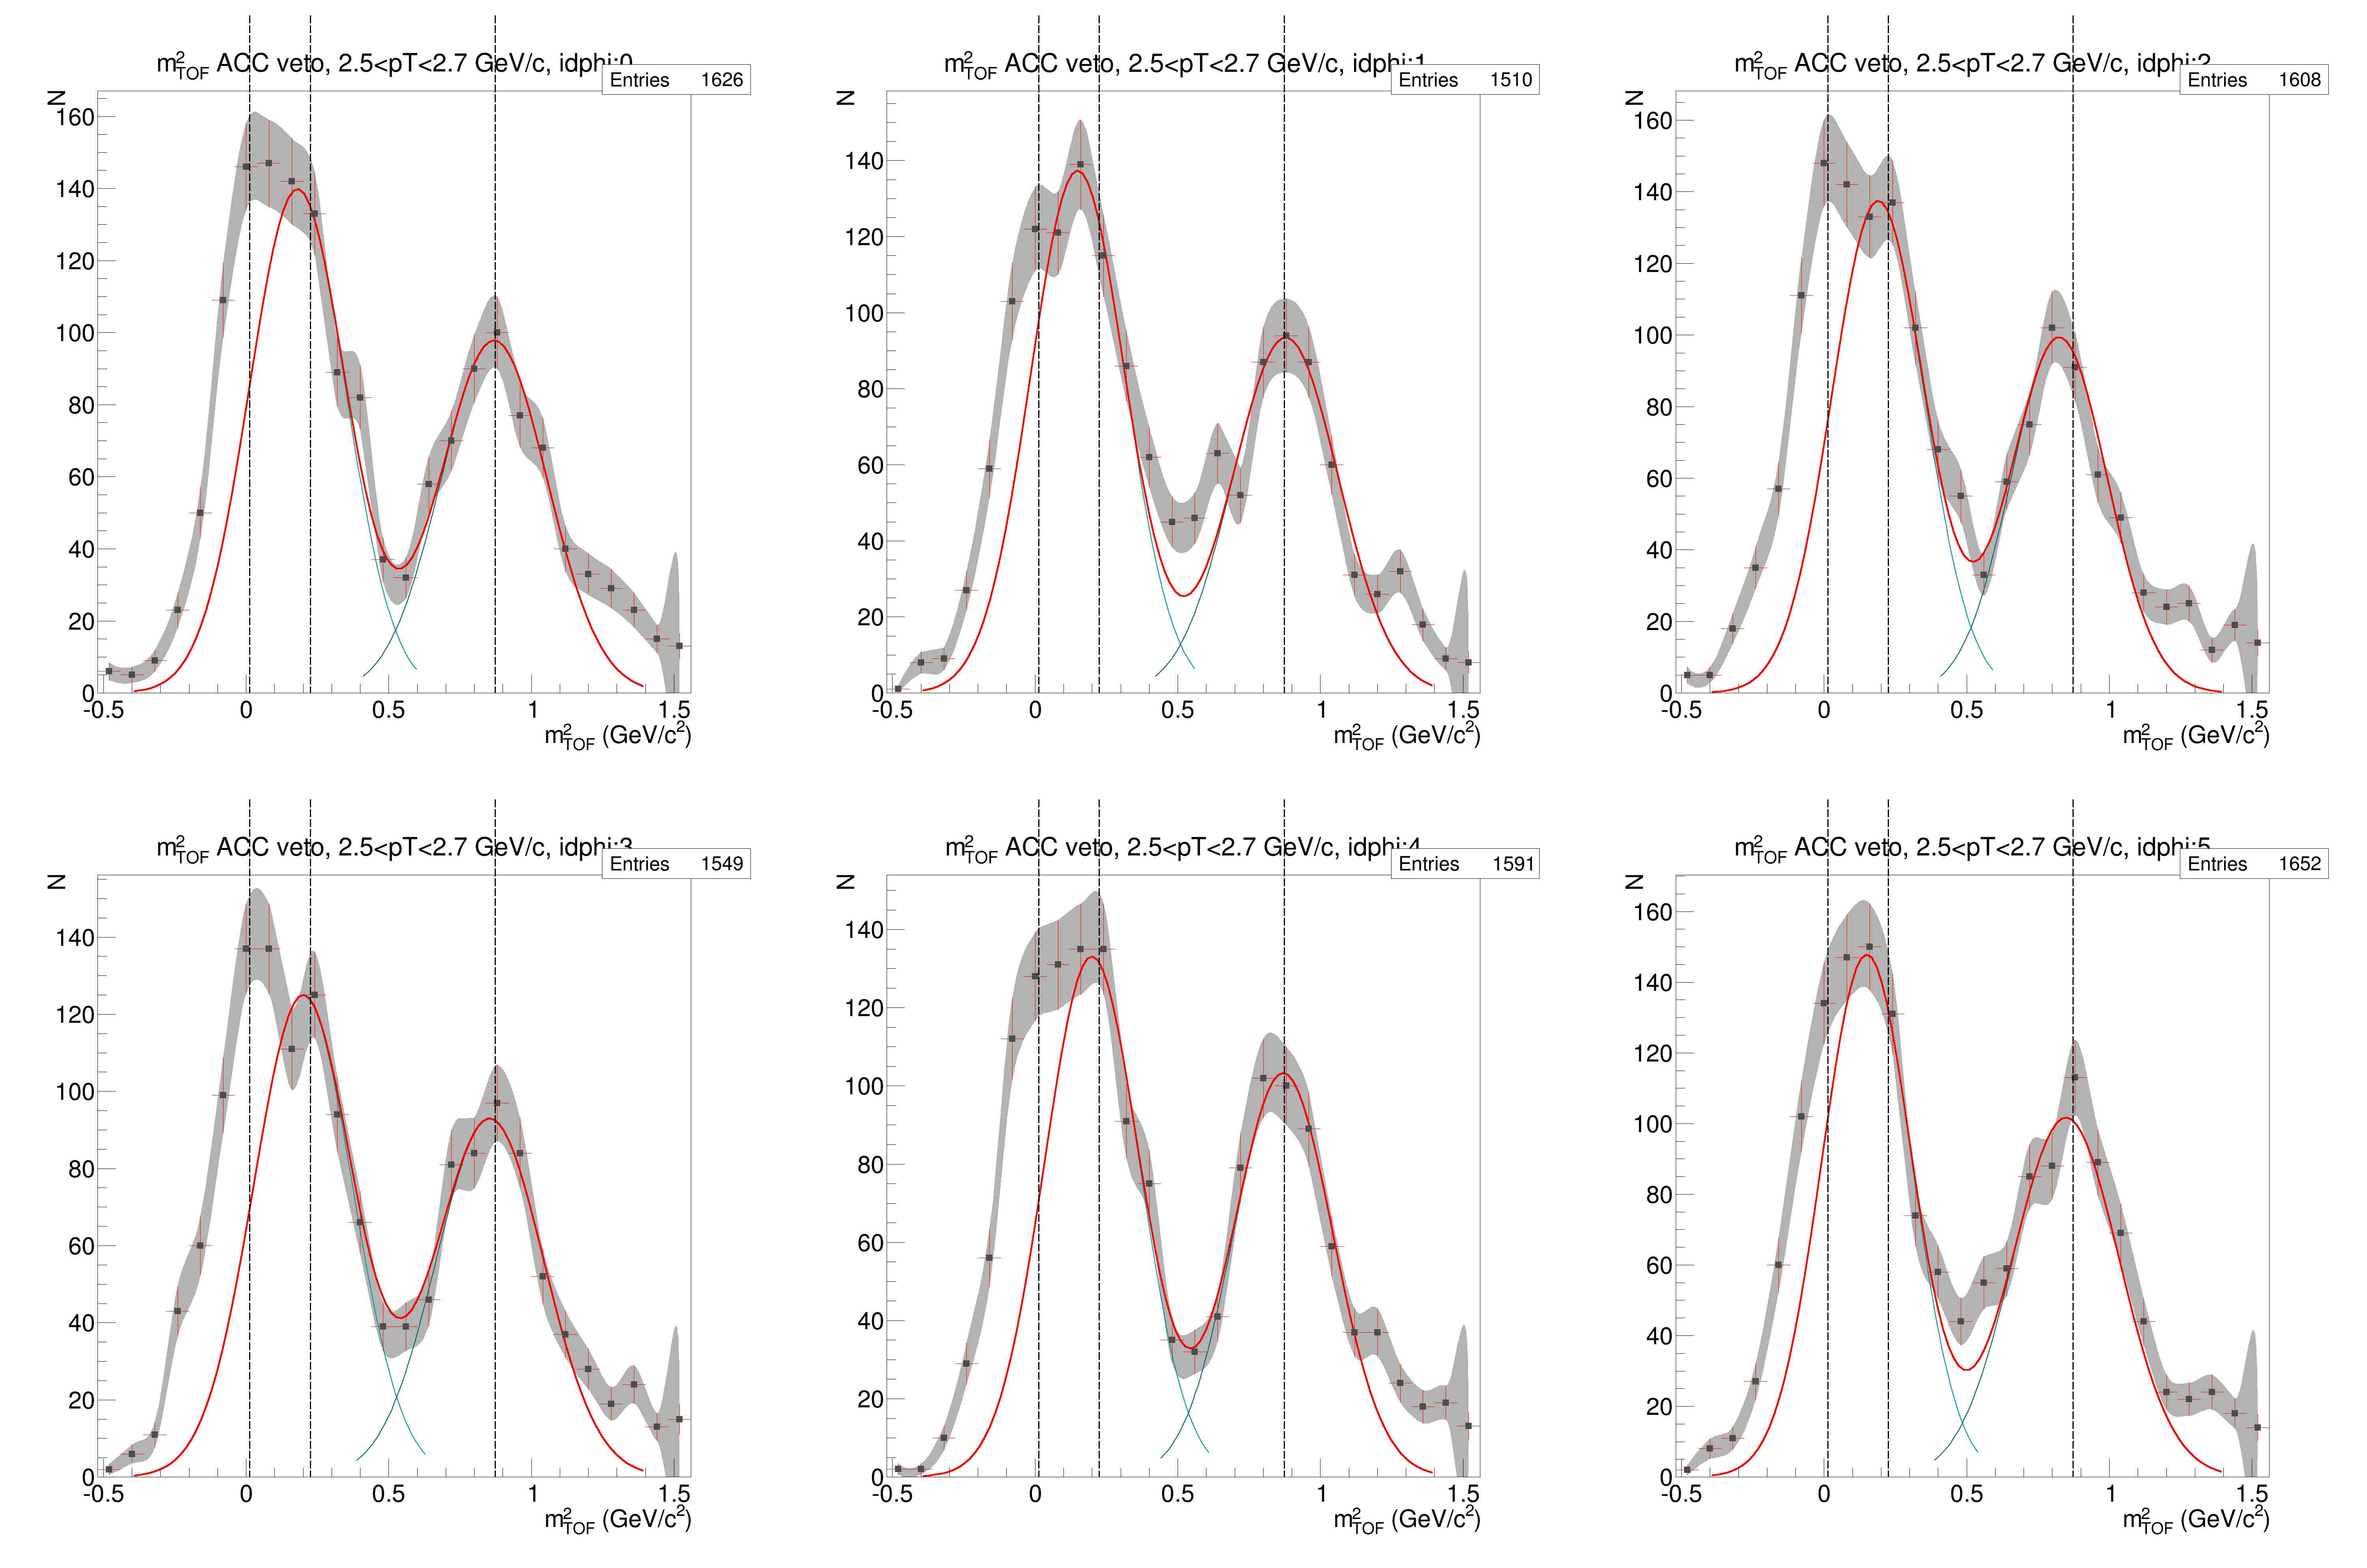
\includegraphics[width=1\textwidth]{hiptfits/neg/PSm2_cent0_ich0_accfire0_ptbin10.jpg}
    \caption{$m^2$ for ACC vetoed tracks}
    \end{subfigure}
    \begin{subfigure}{1\textwidth}
    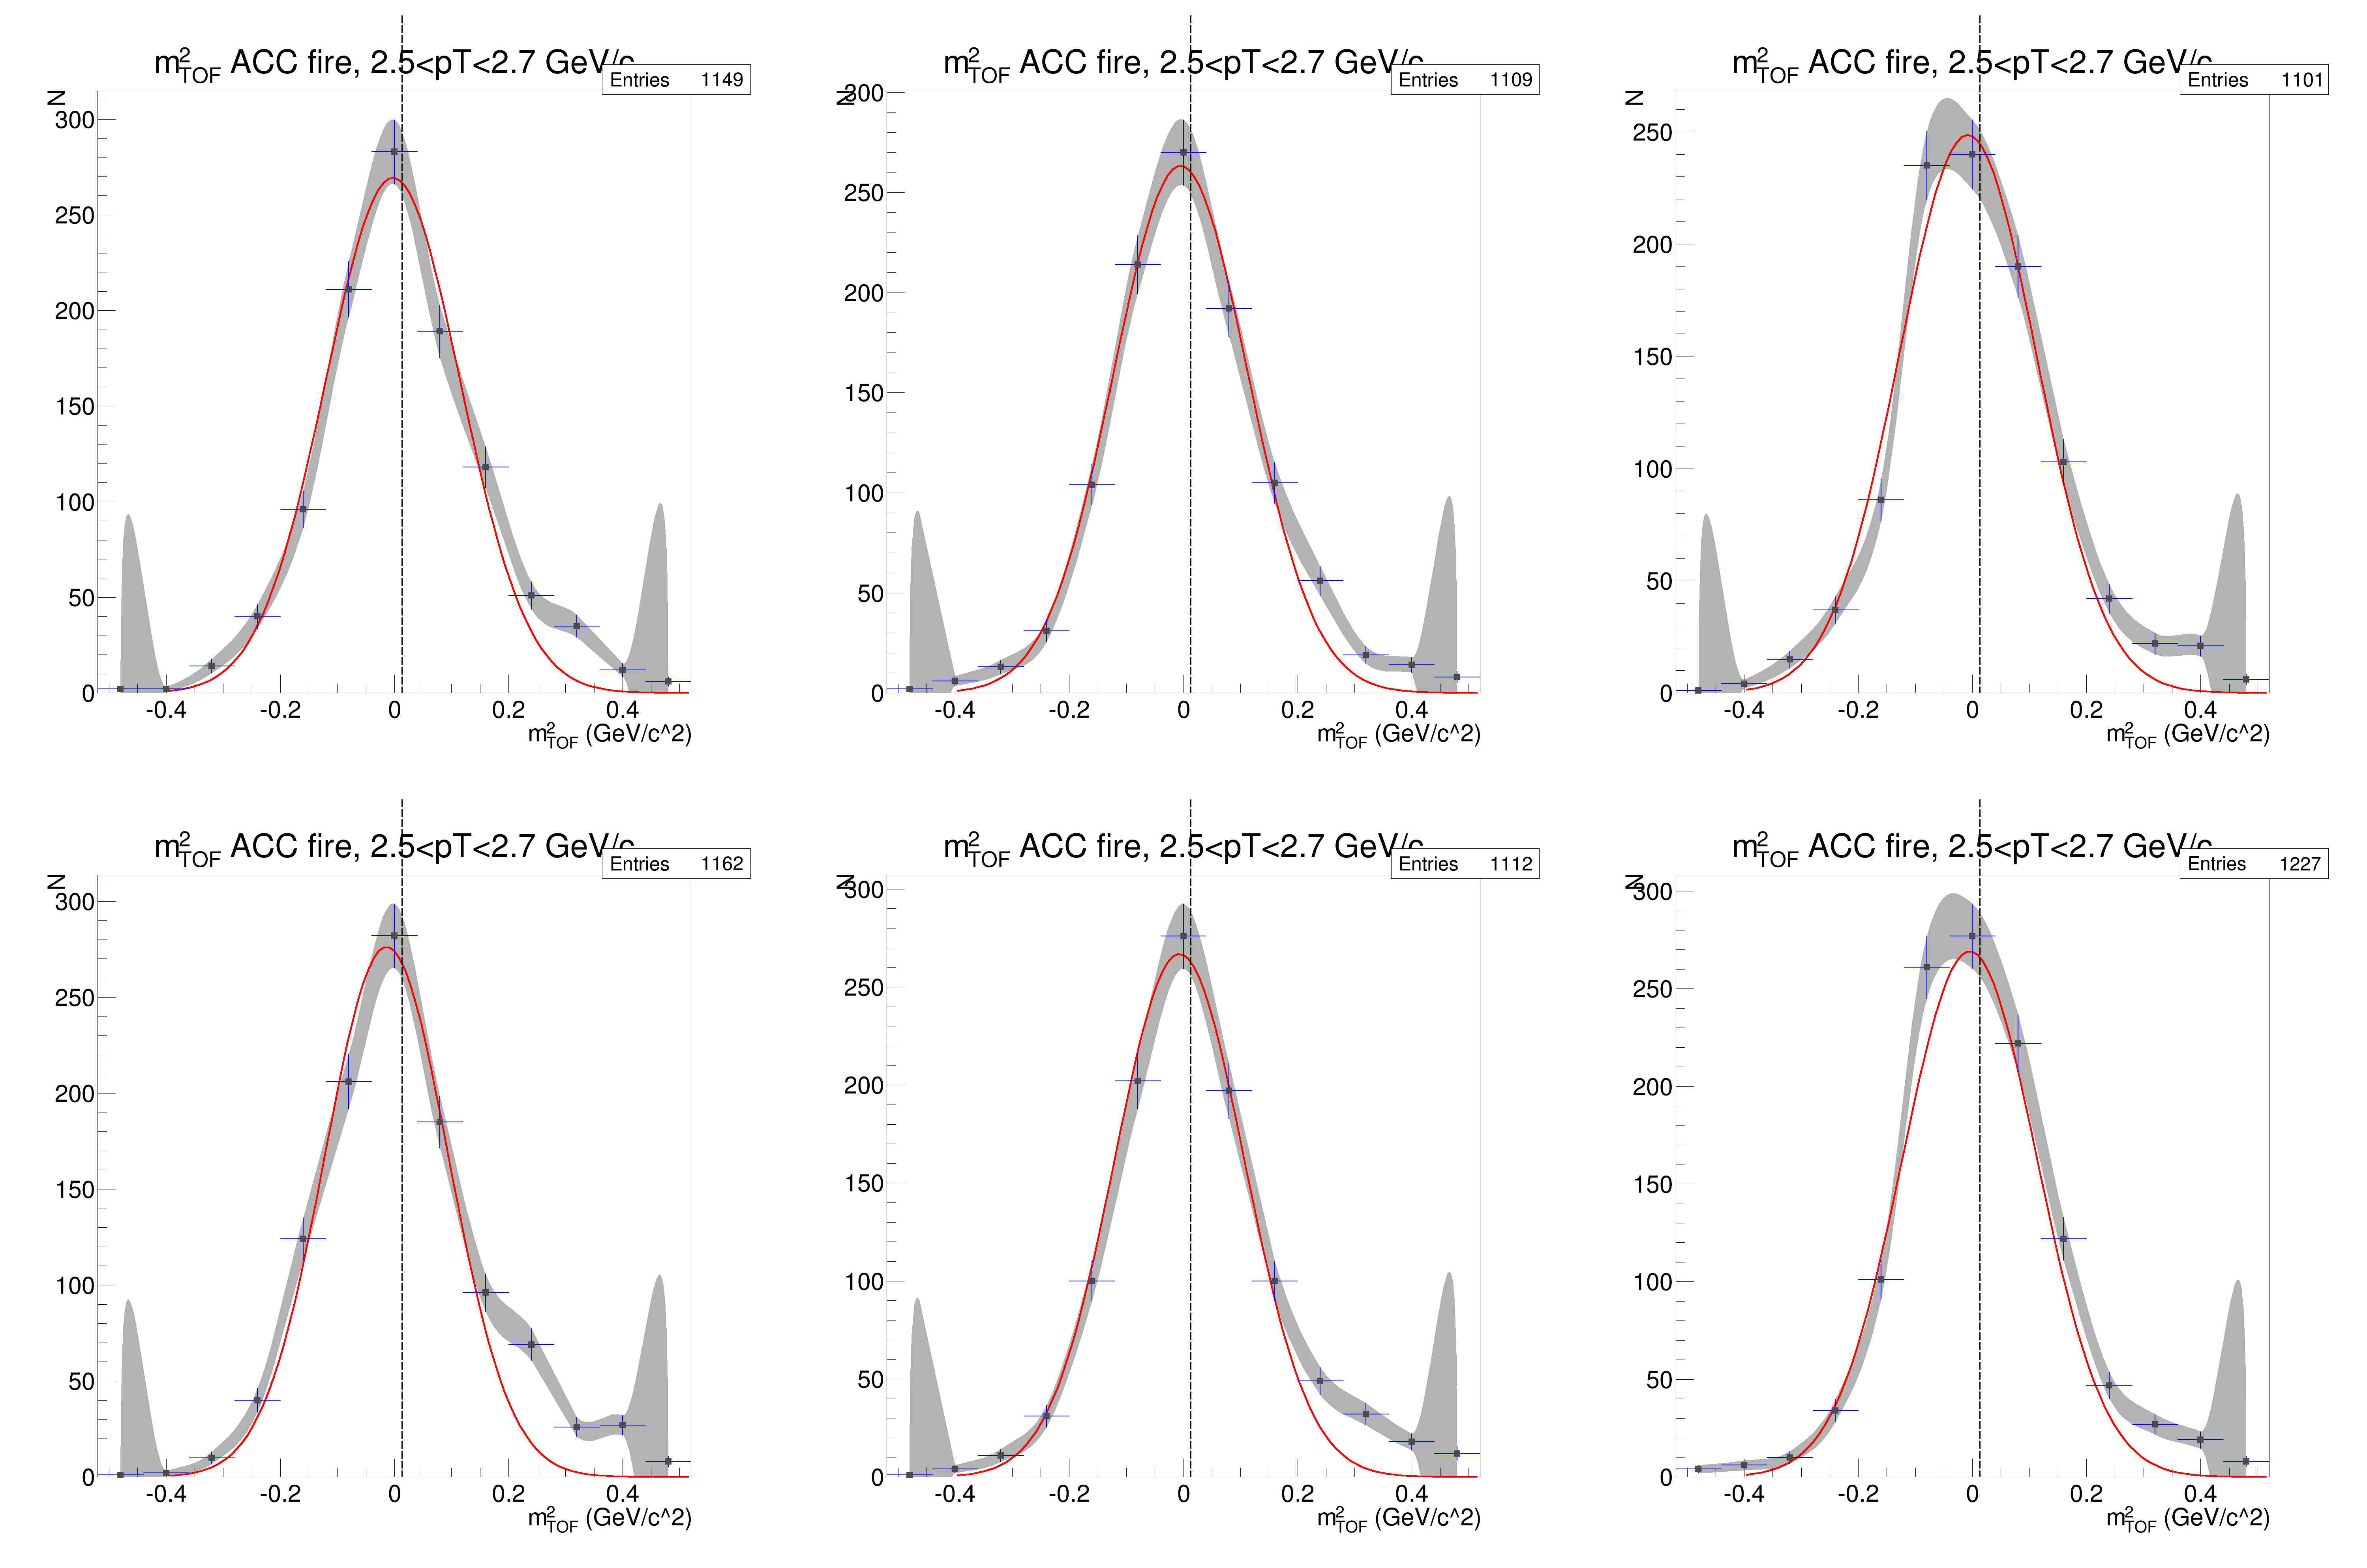
\includegraphics[width=1\textwidth]{hiptfits/neg/PSm2_cent0_ich0_accfire1_ptbin10.jpg}
    \caption{$m^2$ for ACC fired tracks}
    \end{subfigure}  
\end{figure}
\begin{figure}[H]
  \ContinuedFloat
    \begin{subfigure}{1\textwidth}
    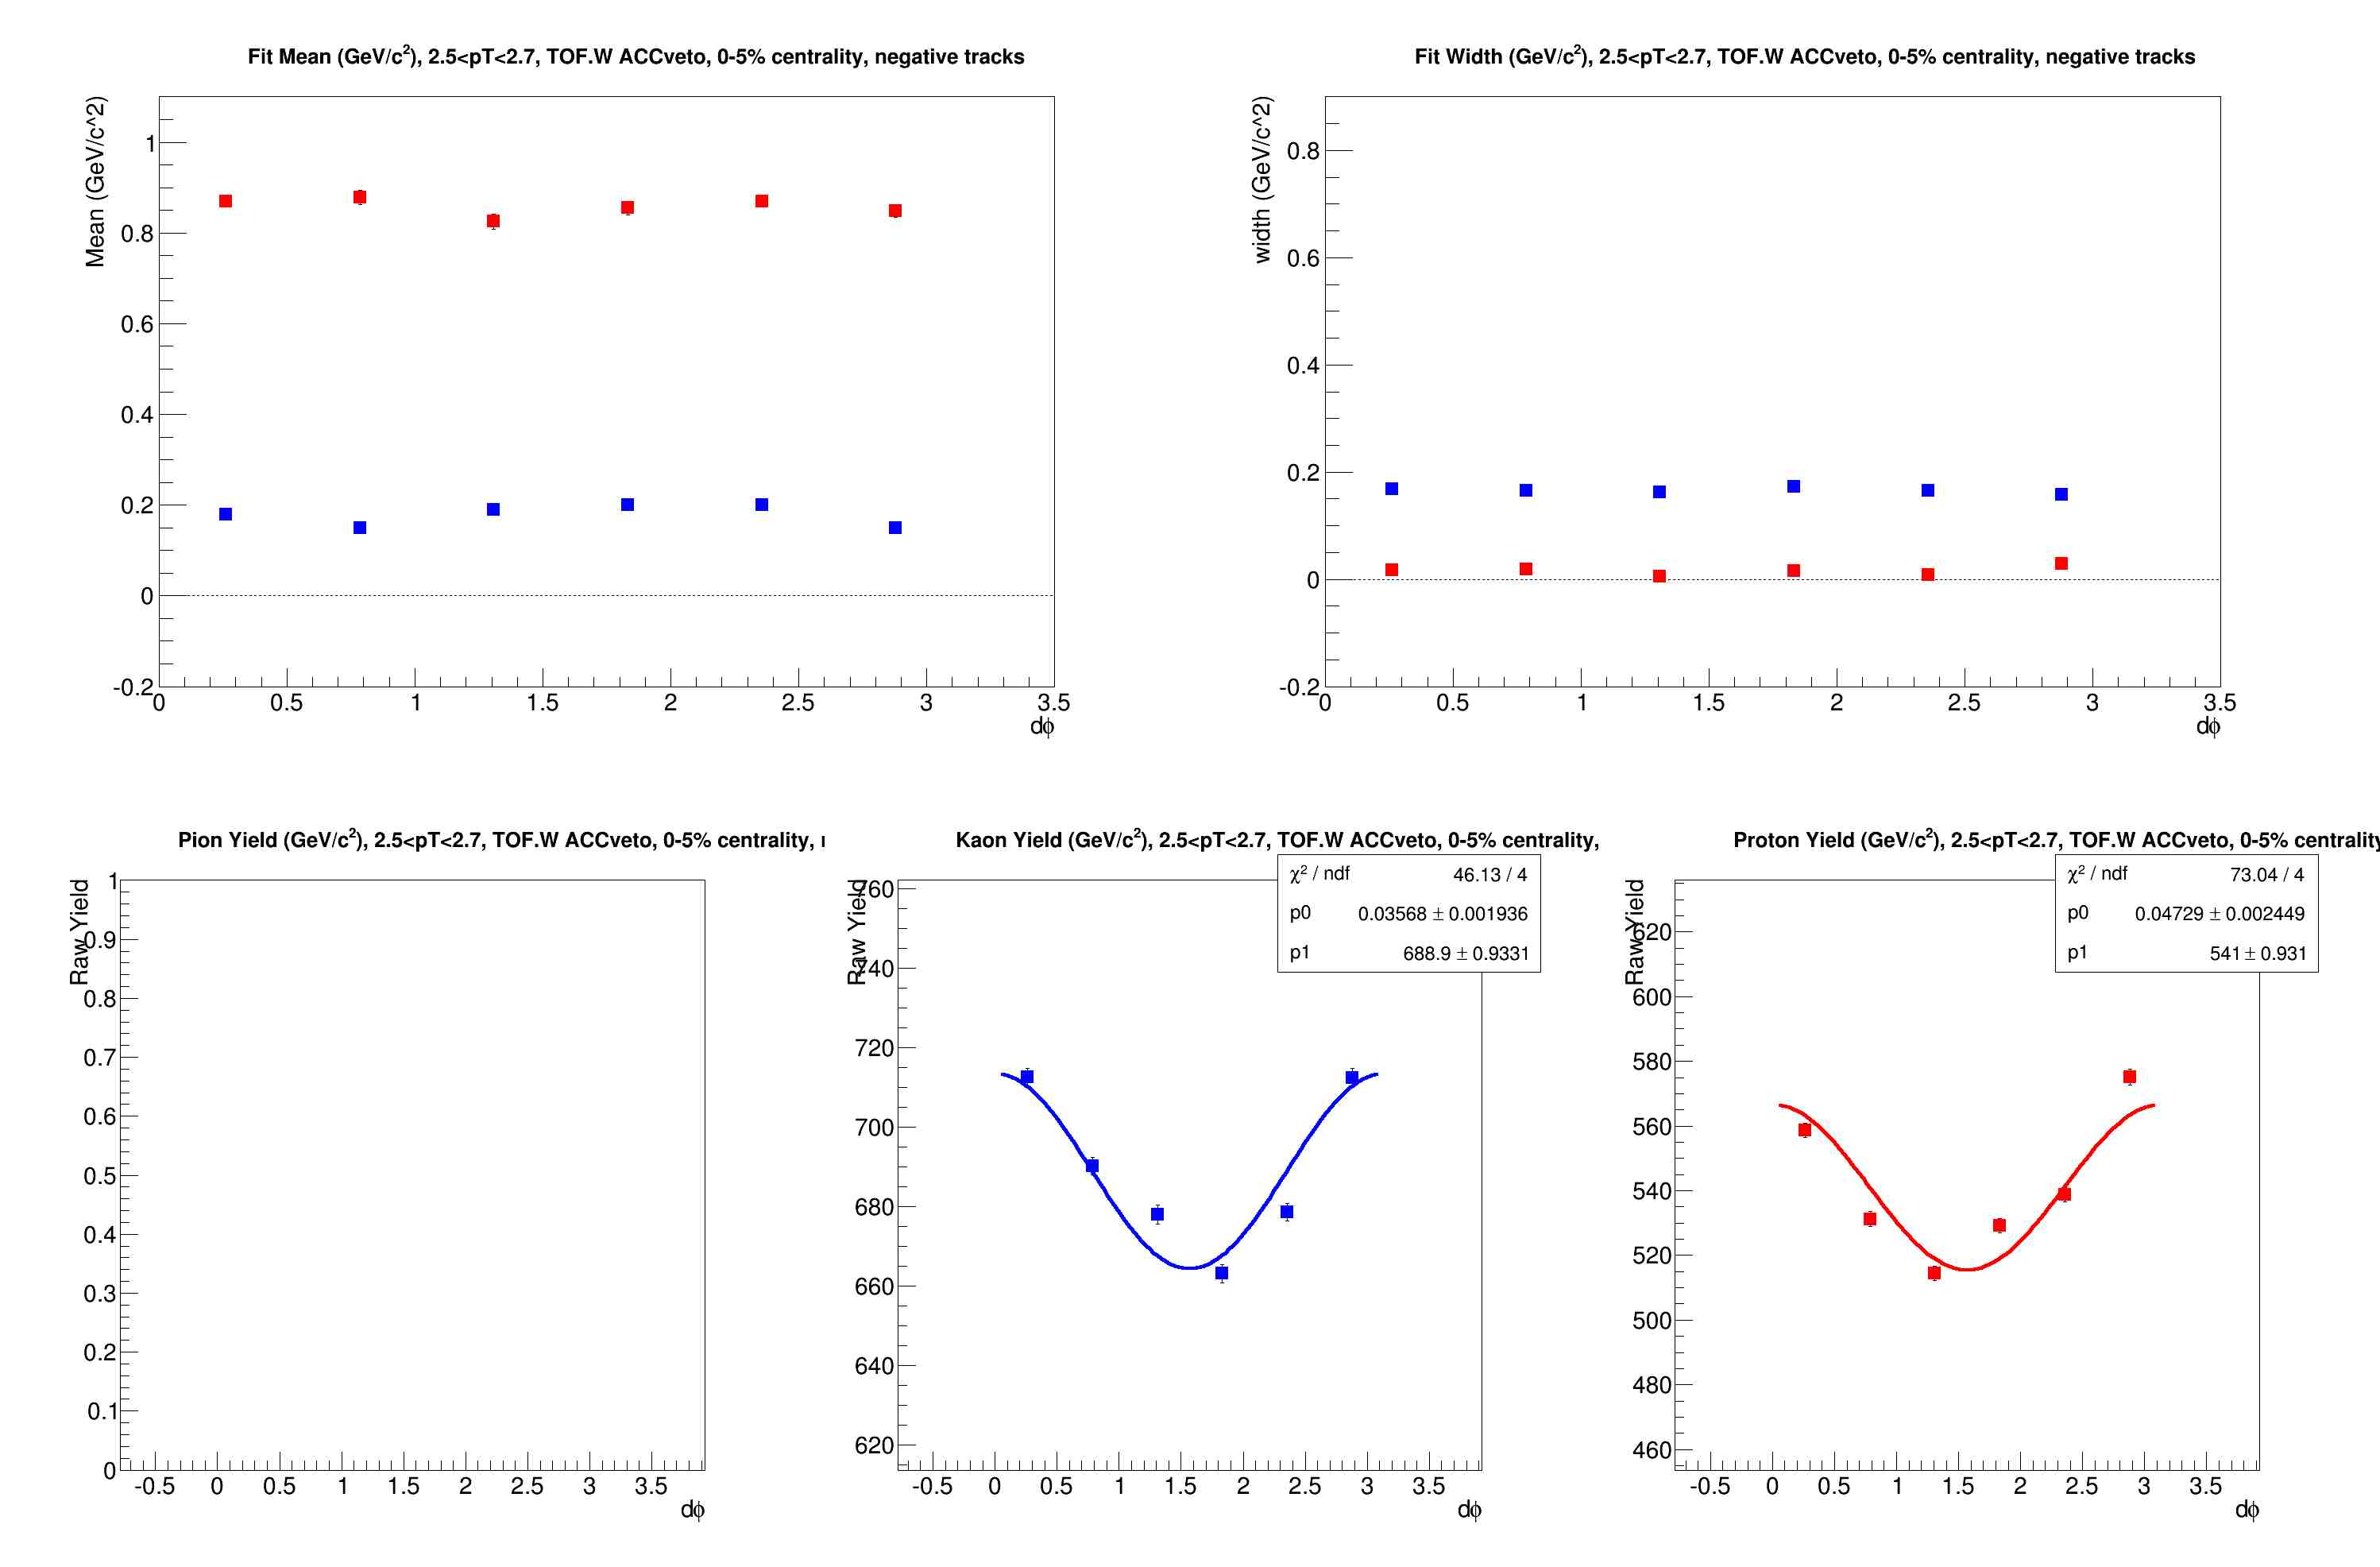
\includegraphics[width=1\textwidth]{hiptfits/neg/fitParams_tof2_cent0_ch0_pT-25-27.jpg}
    \caption{PID parameters and Yields for ACC vetoed tracks}
    \end{subfigure}    
    \begin{subfigure}{1\textwidth}
    \includegraphics[width=1\textwidth]{hiptfits/neg/fitParams_tof3_cent0_ch0_pT-25-27.jpg}
    \caption{PID parameters and Yields for ACC fired tracks}
    \end{subfigure} 
    \rule{35em}{0.5pt}
  \caption[ACC $N_{p.e.}$ vs $m_2$, PID fits, and Yield vs $d\phi$ for $p_T$=2.5-2.7 GeV/c, TOF.W, negative particles]{ACC $N_{p.e.}$ vs $m_2$, PID fits, and Yield vs $d\phi$ for $p_T$=2.5-2.7 GeV/c, TOF.W, negative particles}
  \label{fig:acc25-27neg}
\end{figure}

\begin{figure}[H]
  \centering
    \begin{subfigure}{1\textwidth}
    \includegraphics[width=1\textwidth]{hiptfits/neg/PSaccthreshold_cent0_ich0_accfire0_ptbin11.jpg}
    \caption{$N_{p.e.}$ vs $m^2$}
    \end{subfigure}
\end{figure}
\begin{figure}[H]
  \ContinuedFloat
    \begin{subfigure}{1\textwidth}
    \includegraphics[width=1\textwidth]{hiptfits/neg/PSm2_cent0_ich0_accfire0_ptbin11.jpg}
    \caption{$m^2$ for ACC vetoed tracks}
    \end{subfigure}
    \begin{subfigure}{1\textwidth}
    \includegraphics[width=1\textwidth]{hiptfits/neg/PSm2_cent0_ich0_accfire1_ptbin11.jpg}
    \caption{$m^2$ for ACC fired tracks}
    \end{subfigure}  
\end{figure}
\begin{figure}[H]
  \ContinuedFloat
    \begin{subfigure}{1\textwidth}
    \includegraphics[width=1\textwidth]{hiptfits/neg/fitParams_tof2_cent0_ch0_pT-27-29.jpg}
    \caption{PID parameters and Yields for ACC vetoed tracks}
    \end{subfigure}    
    \begin{subfigure}{1\textwidth}
    \includegraphics[width=1\textwidth]{hiptfits/neg/fitParams_tof3_cent0_ch0_pT-27-29.jpg}
    \caption{PID parameters and Yields for ACC fired tracks}
    \end{subfigure} 
    \rule{35em}{0.5pt}
  \caption[ACC $N_{p.e.}$ vs $m_2$, PID fits, and Yield vs $d\phi$ for $p_T$=2.7-2.9 GeV/c, TOF.W, negative particles]{ACC $N_{p.e.}$ vs $m_2$, PID fits, and Yield vs $d\phi$ for $p_T$=2.7-2.9 GeV/c, TOF.W, negative particles}
  \label{fig:acc27-29neg}
\end{figure}


\begin{figure}[H]
  \centering
    \begin{subfigure}{1\textwidth}
    \includegraphics[width=1\textwidth]{hiptfits/neg/PSaccthreshold_cent0_ich0_accfire0_ptbin12.jpg}
    \caption{$N_{p.e.}$ vs $m^2$}
    \end{subfigure}
\end{figure}
\begin{figure}[H]
  \ContinuedFloat
    \begin{subfigure}{1\textwidth}
    \includegraphics[width=1\textwidth]{hiptfits/neg/PSm2_cent0_ich0_accfire0_ptbin12.jpg}
    \caption{$m^2$ for ACC vetoed tracks}
    \end{subfigure}
    \begin{subfigure}{1\textwidth}
    \includegraphics[width=1\textwidth]{hiptfits/neg/PSm2_cent0_ich0_accfire1_ptbin12.jpg}
    \caption{$m^2$ for ACC fired tracks}
    \end{subfigure}  
\end{figure}
\begin{figure}[H]
  \ContinuedFloat
    \begin{subfigure}{1\textwidth}
    \includegraphics[width=1\textwidth]{hiptfits/neg/fitParams_tof2_cent0_ch0_pT-30-35.jpg}
    \caption{PID parameters and Yields for ACC vetoed tracks}
    \end{subfigure}    
    \begin{subfigure}{1\textwidth}
    \includegraphics[width=1\textwidth]{hiptfits/neg/fitParams_tof3_cent0_ch0_pT-30-35.jpg}
    \caption{PID parameters and Yields for ACC fired tracks}
    \end{subfigure} 
    \rule{35em}{0.5pt}
  \caption[ACC $N_{p.e.}$ vs $m_2$, PID fits, and Yield vs $d\phi$ for $p_T$=3.0-3.5 GeV/c, TOF.W, negative particles]{ACC $N_{p.e.}$ vs $m_2$, PID fits, and Yield vs $d\phi$ for $p_T$=3.0-3.5 GeV/c, TOF.W, negative particles}
  \label{fig:acc30-35neg}
\end{figure}


\subsection{TOF.W and ACC, $p_T$=2.1-3.5 GeV, positive charged tracks}

\begin{figure}[H]
  \centering
    \begin{subfigure}{1\textwidth}
    \includegraphics[width=1\textwidth]{hiptfits/pos/PSaccthreshold_cent0_ich1_accfire0_ptbin8.jpg}
    \caption{$N_{p.e.}$ vs $m^2$}
    \end{subfigure}
\end{figure}
\begin{figure}[H]
  \ContinuedFloat
    \begin{subfigure}{1\textwidth}
    \includegraphics[width=1\textwidth]{hiptfits/pos/PSm2_cent0_ich1_accfire0_ptbin8.jpg}
    \caption{$m^2$ for ACC vetoed tracks}
    \end{subfigure}
    \begin{subfigure}{1\textwidth}
    \includegraphics[width=1\textwidth]{hiptfits/pos/PSm2_cent0_ich1_accfire1_ptbin8.jpg}
    \caption{$m^2$ for ACC fired tracks}
    \end{subfigure}  
\end{figure}
\begin{figure}[H]
  \ContinuedFloat
    \begin{subfigure}{1\textwidth}
    \includegraphics[width=1\textwidth]{hiptfits/pos/fitParams_tof2_cent0_ch1_pT-21-23.jpg}
    \caption{PID parameters and Yields for ACC vetoed tracks}
    \end{subfigure}    
    \begin{subfigure}{1\textwidth}
    \includegraphics[width=1\textwidth]{hiptfits/pos/fitParams_tof3_cent0_ch1_pT-21-23.jpg}
    \caption{PID parameters and Yields for ACC fired tracks}
    \end{subfigure} 
    \rule{35em}{0.5pt}
  \caption[ACC $N_{p.e.}$ vs $m_2$, PID fits, and Yield vs $d\phi$ for $p_T$=2.1-2.3 GeV/c, TOF.W, positive particles]{ACC $N_{p.e.}$ vs $m_2$, PID fits, and Yield vs $d\phi$ for $p_T$=2.1-2.3 GeV/c, TOF.W, positive particles}
  \label{fig:acc21-23pos}
\end{figure}


\begin{figure}[H]
  \centering
    \begin{subfigure}{1\textwidth}
    \includegraphics[width=1\textwidth]{hiptfits/pos/PSaccthreshold_cent0_ich1_accfire0_ptbin9.jpg}
    \caption{$N_{p.e.}$ vs $m^2$}
    \end{subfigure}
\end{figure}
\begin{figure}[H]
  \ContinuedFloat
    \begin{subfigure}{1\textwidth}
    \includegraphics[width=1\textwidth]{hiptfits/pos/PSm2_cent0_ich1_accfire0_ptbin9.jpg}
    \caption{$m^2$ for ACC vetoed tracks}
    \end{subfigure}
    \begin{subfigure}{1\textwidth}
    \includegraphics[width=1\textwidth]{hiptfits/pos/PSm2_cent0_ich1_accfire1_ptbin9.jpg}
    \caption{$m^2$ for ACC fired tracks}
    \end{subfigure}  
\end{figure}
\begin{figure}[H]
  \ContinuedFloat
    \begin{subfigure}{1\textwidth}
    \includegraphics[width=1\textwidth]{hiptfits/pos/fitParams_tof2_cent0_ch1_pT-23-25.jpg}
    \caption{PID parameters and Yields for ACC vetoed tracks}
    \end{subfigure}    
    \begin{subfigure}{1\textwidth}
    \includegraphics[width=1\textwidth]{hiptfits/pos/fitParams_tof3_cent0_ch1_pT-23-25.jpg}
    \caption{PID parameters and Yields for ACC fired tracks}
    \end{subfigure} 
    \rule{35em}{0.5pt}
  \caption[ACC $N_{p.e.}$ vs $m_2$, PID fits, and Yield vs $d\phi$ for $p_T$=2.3-2.5 GeV/c, TOF.W, positive particles]{ACC $N_{p.e.}$ vs $m_2$, PID fits, and Yield vs $d\phi$ for $p_T$=2.3-2.5 GeV/c, TOF.W, positive particles}
  \label{fig:acc23-25pos}
\end{figure}


\begin{figure}[H]
  \centering
    \begin{subfigure}{1\textwidth}
    \includegraphics[width=1\textwidth]{hiptfits/pos/PSaccthreshold_cent0_ich1_accfire0_ptbin10.jpg}
    \caption{$N_{p.e.}$ vs $m^2$}
    \end{subfigure}
\end{figure}
\begin{figure}[H]
  \ContinuedFloat
    \begin{subfigure}{1\textwidth}
    \includegraphics[width=1\textwidth]{hiptfits/pos/PSm2_cent0_ich1_accfire0_ptbin10.jpg}
    \caption{$m^2$ for ACC vetoed tracks}
    \end{subfigure}
    \begin{subfigure}{1\textwidth}
    \includegraphics[width=1\textwidth]{hiptfits/pos/PSm2_cent0_ich1_accfire1_ptbin10.jpg}
    \caption{$m^2$ for ACC fired tracks}
    \end{subfigure}  
\end{figure}
\begin{figure}[H]
  \ContinuedFloat
    \begin{subfigure}{1\textwidth}
    \includegraphics[width=1\textwidth]{hiptfits/pos/fitParams_tof2_cent0_ch1_pT-25-27.jpg}
    \caption{PID parameters and Yields for ACC vetoed tracks}
    \end{subfigure}    
    \begin{subfigure}{1\textwidth}
    \includegraphics[width=1\textwidth]{hiptfits/pos/fitParams_tof3_cent0_ch1_pT-25-27.jpg}
    \caption{PID parameters and Yields for ACC fired tracks}
    \end{subfigure} 
    \rule{35em}{0.5pt}
  \caption[ACC $N_{p.e.}$ vs $m_2$, PID fits, and Yield vs $d\phi$ for $p_T$=2.5-2.7 GeV/c, TOF.W, negative particles]{ACC $N_{p.e.}$ vs $m_2$, PID fits, and Yield vs $d\phi$ for $p_T$=2.5-2.7 GeV/c, TOF.W, positive particles}
  \label{fig:acc25-27pos}
\end{figure}

\begin{figure}[H]
  \centering
    \begin{subfigure}{1\textwidth}
    \includegraphics[width=1\textwidth]{hiptfits/pos/PSaccthreshold_cent0_ich1_accfire0_ptbin11.jpg}
    \caption{$N_{p.e.}$ vs $m^2$}
    \end{subfigure}
\end{figure}
\begin{figure}[H]
  \ContinuedFloat
    \begin{subfigure}{1\textwidth}
    \includegraphics[width=1\textwidth]{hiptfits/pos/PSm2_cent0_ich1_accfire0_ptbin11.jpg}
    \caption{$m^2$ for ACC vetoed tracks}
    \end{subfigure}
    \begin{subfigure}{1\textwidth}
    \includegraphics[width=1\textwidth]{hiptfits/pos/PSm2_cent0_ich1_accfire1_ptbin11.jpg}
    \caption{$m^2$ for ACC fired tracks}
    \end{subfigure}  
\end{figure}
\begin{figure}[H]
  \ContinuedFloat
    \begin{subfigure}{1\textwidth}
    \includegraphics[width=1\textwidth]{hiptfits/pos/fitParams_tof2_cent0_ch1_pT-27-29.jpg}
    \caption{PID parameters and Yields for ACC vetoed tracks}
    \end{subfigure}    
    \begin{subfigure}{1\textwidth}
    \includegraphics[width=1\textwidth]{hiptfits/pos/fitParams_tof3_cent0_ch1_pT-27-29.jpg}
    \caption{PID parameters and Yields for ACC fired tracks}
    \end{subfigure} 
    \rule{35em}{0.5pt}
  \caption[ACC $N_{p.e.}$ vs $m_2$, PID fits, and Yield vs $d\phi$ for $p_T$=2.7-2.9 GeV/c, TOF.W, positive particles]{ACC $N_{p.e.}$ vs $m_2$, PID fits, and Yield vs $d\phi$ for $p_T$=2.7-2.9 GeV/c, TOF.W, positive particles}
  \label{fig:acc27-29pos}
\end{figure}


\begin{figure}[H]
  \centering
    \begin{subfigure}{1\textwidth}
    \includegraphics[width=1\textwidth]{hiptfits/pos/PSaccthreshold_cent0_ich1_accfire0_ptbin12.jpg}
    \caption{$N_{p.e.}$ vs $m^2$}
    \end{subfigure}
\end{figure}
\begin{figure}[H]
  \ContinuedFloat
    \begin{subfigure}{1\textwidth}
    \includegraphics[width=1\textwidth]{hiptfits/pos/PSm2_cent0_ich1_accfire0_ptbin12.jpg}
    \caption{$m^2$ for ACC vetoed tracks}
    \end{subfigure}
    \begin{subfigure}{1\textwidth}
    \includegraphics[width=1\textwidth]{hiptfits/pos/PSm2_cent0_ich1_accfire1_ptbin12.jpg}
    \caption{$m^2$ for ACC fired tracks}
    \end{subfigure}  
\end{figure}
\begin{figure}[H]
  \ContinuedFloat
    \begin{subfigure}{1\textwidth}
    \includegraphics[width=1\textwidth]{hiptfits/pos/fitParams_tof2_cent0_ch1_pT-30-35.jpg}
    \caption{PID parameters and Yields for ACC vetoed tracks}
    \end{subfigure}    
    \begin{subfigure}{1\textwidth}
    \includegraphics[width=1\textwidth]{hiptfits/pos/fitParams_tof3_cent0_ch1_pT-30-35.jpg}
    \caption{PID parameters and Yields for ACC fired tracks}
    \end{subfigure} 
    \rule{35em}{0.5pt}
  \caption[ACC $N_{p.e.}$ vs $m_2$, PID fits, and Yield vs $d\phi$ for $p_T$=3.0-3.5 GeV/c, TOF.W, positive particles]{ACC $N_{p.e.}$ vs $m_2$, PID fits, and Yield vs $d\phi$ for $p_T$=3.0-3.5 GeV/c, TOF.W, positive particles}
  \label{fig:acc30-35pos}
\end{figure}

\restoregeometry



\begin{table}
\end{table}